\documentclass[12pt,a4paper,oneside]{report}

% --- Encoding & language ---
\usepackage[utf8]{inputenc}
\usepackage[T1]{fontenc}
\usepackage[english]{babel}

% --- Fonts: Times-like, math-compatible ---
\usepackage{mathptmx}

% --- Geometry: Bocconi-style margins ---
\usepackage[
  left=2.5cm, right=2.5cm, top=3.2cm, bottom=2.54cm
]{geometry}

% --- Spacing ---
\usepackage{setspace}
\setstretch{1.3}
\setlength{\parindent}{1.27cm}

% --- Loosen line-breaking tolerance to absorb compound-word overflow
%     (de-commodification, Mediterranean-familistic, digital-engagement-anchored,
%      etc.) without ugly per-word \hyphenation hints.
\setlength{\emergencystretch}{3em}

% --- Tables, figures, math ---
\usepackage{booktabs}
\usepackage{longtable}
\usepackage{tikz}
\usetikzlibrary{positioning, arrows.meta, shapes.geometric, fit}
\usepackage{array}
\usepackage{multirow}
\usepackage{graphicx}
\usepackage{float}
\usepackage[section]{placeins}
\usepackage{tabularx}
\usepackage{threeparttable}
\usepackage{caption}
\usepackage{subcaption}
\captionsetup{font=small, labelfont=bf}

% --- Permissive float placement to avoid mid-page gaps ---
\renewcommand{\topfraction}{0.9}
\renewcommand{\bottomfraction}{0.8}
\renewcommand{\textfraction}{0.07}
\renewcommand{\floatpagefraction}{0.7}
\setcounter{topnumber}{3}
\setcounter{bottomnumber}{3}
\setcounter{totalnumber}{4}
% Top-align figures on dedicated float pages (e.g. full-UI screenshots in Ch.8):
% without this, a lone figure on a float page is vertically centred, leaving
% white space both above and below. These lengths anchor it to the top.
\makeatletter
\setlength{\@fptop}{0pt}
\setlength{\@fpsep}{12pt plus 1fil}
\setlength{\@fpbot}{0pt plus 1fil}
\makeatother
\usepackage{amsmath, amssymb}

% --- Hyperlinks & TOC ---
% colorlinks with everything black by default (same look as hidelinks for TOC,
% cross-references and citations), then only external URLs are tinted below.
\usepackage[colorlinks=true, allcolors=black, breaklinks=true]{hyperref}
\hypersetup{
  pdftitle={Invisible Profiles: A Multidimensional Segmentation of the Over-65 Population in Italy and Sweden --- Evidence from SHARE Wave 9},
  pdfsubject={MSc Thesis, Bocconi University, MSc EMIT, AY 2025--2026},
  pdfkeywords={multidimensional segmentation; older adults; SHARE Wave 9; welfare regimes; cross-country comparison; Italy; Sweden; silver economy; subjective well-being; K-means; Latent Class Analysis}
}

% --- Code listings (R) ---
\usepackage{xcolor}
\definecolor{thesisaccent}{HTML}{185FA5} % accent for comparison-table dividers/headers
% Tint only external hyperlinks (\href / \url) in the thesis-accent blue, so the
% data/code-availability links are visibly clickable while internal links stay black.
\hypersetup{urlcolor=thesisaccent}
\usepackage{listings}
\lstset{
  language=R,
  basicstyle=\ttfamily\footnotesize,
  keywordstyle=\color{blue!70!black}\bfseries,
  commentstyle=\color{green!40!black}\itshape,
  stringstyle=\color{purple!70!black},
  numbers=left, numberstyle=\tiny\color{gray}, stepnumber=1, numbersep=8pt,
  showstringspaces=false,
  breaklines=true, breakatwhitespace=true,
  frame=single, framesep=4pt, framerule=0.4pt, rulecolor=\color{gray!30},
  tabsize=2, columns=fullflexible, keepspaces=true
}
% Map R's assignment operator to a proper leftarrow glyph in listings.
% Note: we do NOT map '%' here (biblatex's apa style and the literate
% parser cannot both parse a bare '%' inside braces without escaping the
% LaTeX comment character).
\lstset{literate={<-}{$\leftarrow$}{2}}

% --- Bibliography (biblatex + biber, APA style) ---
\usepackage{csquotes}  % required by biblatex when babel/polyglossia is loaded
\usepackage[
  style=apa,
  backend=biber,
  natbib=true,
  url=false,
  doi=false,
  isbn=false
]{biblatex}
\addbibresource{references.bib}

% --- Chapter title page + per-chapter footer ---
\usepackage{fancyhdr}
\usepackage{etoolbox}
\usepackage{refcount}

\newif\ifchaptertitlepageinit
\chaptertitlepageinitfalse

\newcommand{\saferef}[1]{\getpagerefnumber{#1}}

\renewcommand{\chaptermark}[1]{\markboth{#1}{}}

\newcommand{\chapfooterline}{%
  \small Chapter \thechapter\ --- \leftmark\,$\cdot$\,Page \thepage%
}

\fancypagestyle{plain}{%
  \fancyhf{}%
  \renewcommand{\headrulewidth}{0pt}%
  \renewcommand{\footrulewidth}{0pt}%
  \fancyfoot[C]{\chapfooterline}%
}

\pagestyle{fancy}
\fancyhf{}
\renewcommand{\headrulewidth}{0pt}
\renewcommand{\footrulewidth}{0pt}
\fancyfoot[C]{\chapfooterline}

\newcommand{\chaptertitlepage}[2]{%
  \ifchaptertitlepageinit
    \closelastchapter
    \global\chapendlabeledfalse
  \fi
  \cleardoublepage
  % Numbering is arabic and continuous from the frontmatter (Bocconi §10.3.1);
  % Chapter 1 does NOT reset to page 1. \cleardoublepage still forces an
  % odd (right-hand) opening page.
  \refstepcounter{chapter}%
  \chaptermark{#1}%
  \phantomsection
  \addcontentsline{toc}{chapter}{\protect\numberline{\thechapter}#1}%
  \label{chap:\thechapter:start}%
  \thispagestyle{plain}%
  % Compact chapter opening — no full title page.
  \vspace*{1.2cm}
  \noindent{\large\bfseries Chapter \thechapter\par}
  \vspace{0.4cm}
  \noindent{\Huge\bfseries #1\par}
  \vspace{0.3cm}
  \noindent{\large\itshape #2\par}
  \vspace{1.2cm}
}

\newif\ifchapendlabeled
\chapendlabeledfalse
\newcommand{\closelastchapter}{%
  \ifchapendlabeled\else
    \label{chap:\thechapter:end}%
    \global\chapendlabeledtrue
  \fi
}
\AtEndDocument{\closelastchapter}

% Bibliography: redefine 'plain' inside pretocmd so biblatex's \chapter*
% picks up a page-number-only footer (no Chapter X — Page N of M).
\pretocmd{\printbibliography}{%
  \closelastchapter
  \fancypagestyle{plain}{%
    \fancyhf{}%
    \renewcommand{\headrulewidth}{0pt}%
    \renewcommand{\footrulewidth}{0pt}%
    \fancyfoot[C]{\small\thepage}%
  }%
  \pagestyle{plain}%
}{}{}

% --- Document ---
\title{Invisible Profiles: A Multidimensional Segmentation of the Over-65 Population in Italy and Sweden --- Evidence from SHARE Wave 9}
\author{}
\date{Academic Year 2025--2026}

\begin{document}

% ===== Frontmatter =====
% No title page and no abstract in the PDF: Bocconi prints the title page
% automatically from the online data, and the abstract is typed online
% (max 4,000 chars). See frontmatter/abstract.tex for the text to paste.

% Override 'plain' to a simple page-number footer (the chapter-aware
% \chapfooterline embeds Chapter X / \leftmark, undefined in the frontmatter).
\fancypagestyle{plain}{%
  \fancyhf{}%
  \renewcommand{\headrulewidth}{0pt}%
  \renewcommand{\footrulewidth}{0pt}%
  \fancyfoot[C]{\small\thepage}%
}

% Bocconi MSc 2025-26 §10.3.1: 4 mandatory leading pages, arabic numbering throughout
\pagenumbering{arabic}
\setcounter{page}{1}
\pagestyle{plain}

% The 4 mandatory leading pages can be suppressed for the native-link variant
% (\def\nofrontblanks{1}); page counter jumps to 5 so printed folios stay 5->101.
\ifdefined\nofrontblanks
  \setcounter{page}{5}%
\else
% Page 1: blank
\thispagestyle{empty}\null\clearpage
% Page 2: blank
\thispagestyle{empty}\null\clearpage
% Page 3: acknowledgments (placeholder; Vincenzo will fill before final submission)
\thispagestyle{empty}
\vspace*{2.5cm}
\begin{center}
  {\Large\bfseries Ringraziamenti}
\end{center}
\vspace{0.6cm}

\noindent Colgo questa pagina per fermare, brevemente, gli ultimi due anni --- e le persone
e i momenti che li hanno attraversati.

\medskip
\noindent Sono stati anni importanti, dentro e fuori l'università. Ne conservo immagini
spensierate: le giornate australiane passate a decidere cosa avremmo visitato, i pomeriggi
milanesi del dopo-esame a chiacchierare al bar. E frangenti in cui ho dovuto impegnarmi
davvero: le giornate lunghissime prima degli esami, passate a fare e rifare il giro del
programma, e i cinque esami in trenta giorni della prima sessione, che ricordo bene. Nel
complesso, di questo tempo porto con me un ricordo positivo, che mi ha arricchito.

\medskip
\noindent Tutto ciò che faccio, però, poggia sul sostegno della mia \textbf{famiglia}. Sono
sempre stato un ragazzo a cui la realtà di paese andava stretta, e ho sempre cercato di
andare oltre --- per curiosità, e per mettermi in gioco. La mia \textbf{famiglia} non mi ha
mai fatto mancare né i mezzi né il supporto per farlo. Non tutti possono dirlo: io sì, e
non lo do per scontato.

\medskip
\noindent Un grazie a tutte le persone che hanno fatto parte di questi due anni accademici:
i professori, i compagni, ma anche chi ha condiviso soltanto una conversazione nata per
caso, a Milano, ad Adelaide o ovunque sia capitato. Alcune di quelle conversazioni mi sono
rimaste impresse più di altre, ma tutte fanno parte del percorso, e lo hanno reso più ricco
e più interessante.

\medskip
\noindent Menzione d'onore, infine, per la mia cagnolina \textbf{Hope}, a cui voglio un
bene enorme: sono felice che sia stata accanto a me e alla mia \textbf{famiglia} in questi
anni. Ha reso tutto molto più bello.

\clearpage
% Page 4: blank
\thispagestyle{empty}\null\clearpage
\fi

% From page 5: TOC, LoF, LoT
\tableofcontents
\clearpage
\listoffigures
\clearpage
\listoftables
\clearpage

% ===== Mainmatter =====
% Restore the chapter-aware 'plain' (used by \chaptertitlepage and \chapter*).
\fancypagestyle{plain}{%
  \fancyhf{}%
  \renewcommand{\headrulewidth}{0pt}%
  \renewcommand{\footrulewidth}{0pt}%
  \fancyfoot[C]{\chapfooterline}%
}
\setcounter{chapter}{0}  % forces next \chapter to be numbered 1
\chapter{The Italian Silver Economy and the Cost of an Unsegmented Market}
\label{ch:ch1}

\section{A demographic transformation with an economic price tag}
Italy is ageing faster than almost any other country in the European Union and at a pace that decisively reframes its over-65 population from a fiscal and clinical liability into the largest single addressable consumer segment of the next two decades. According to Istat (2024), roughly 14.2~million Italian residents were aged 65 or older at the start of 2024, equivalent to 23.8\% of the total population and the second-highest share among the EU-27 after Germany. Eurostat projects this share to reach 30\% by 2050, with the old-age dependency ratio rising from 37.5 to 60. The European Commission's silver-economy reports (European Commission, 2018, 2021) estimate that the EU's 50-plus segment already generates a quarter of total EU GDP through consumption and that its real spending power has been growing faster than the rest of the population's for the last decade. In Italy alone, the over-65 segment commanded approximately \texteuro{}243.8~billion in aggregate annual household income flow and approximately \texteuro{}2.33~trillion in household net wealth in 2024, computed as Istat over-65 individual counts multiplied by SHARE Wave~9 median household figures.

This is the silver economy. It is the largest customer base of contemporary Italian capitalism, and unlike younger demographic blocks it is not declining: the segment that funds private pensions, owns the housing stock, sits on the financial assets, and consumes a disproportionate share of healthcare, financial advisory and personal-services markets is structurally expanding through 2050. For a country whose macroeconomic growth is constrained by labour-force decline, the productivity of the silver-economy segment --- the efficiency with which markets serve it --- is increasingly indistinguishable from the productivity of the economy as a whole.

\section{The system treats the segment as a monolith. It is not.}
Despite the segment's economic significance, Italian commercial and public services continue to address the over-65 population as if it were a single homogeneous block defined by age. Insurance companies design "senior" products tailored to a stylised retiree; banks deploy generic "wealth preservation" packages; the public administration plans elderly services from aggregate municipal head-counts; pharmaceutical and OTC operators run age-band marketing campaigns that ignore the substantial heterogeneity of digital reach and engagement within the cohort. The premise of this thesis is that this monolithic treatment is both behaviourally wrong and economically inefficient.

The heterogeneity is empirically large. Among Italians aged 65 and over, internet penetration in 2021--2022 ranged from 9\% in the most isolated profile to 75\% in the most digitally engaged; financial distress affected roughly half of one segment and almost no respondents in another; quality of life as measured by the CASP-12 scale spanned more than ten points across profiles within the same country, age group and clinical condition. A "senior" insurance product positioned for the average over-65 customer is a product positioned for nobody in particular: it under-serves the digital high-income segment that wants self-managed online onboarding, fails the asset-rich socially-isolated segment that needs human-mediated navigation, and prices uncompetitively for the fragile lower-income segment whose actual willingness-to-pay is below the average premium.

The cost of this misalignment is observable in two ways that this thesis quantifies in subsequent chapters. The first is healthcare under-utilisation. Italy's over-65 population pays for routine general-practitioner contact at a rate comparable to Sweden's but uses preventive services --- dental care, elective specialist consultation, screening --- at a fraction of the Swedish rate (Italy 30\% twelve-month dentist contact against Sweden 84\%). Within Italy, this preventive-care deficit concentrates in a profile whose objective conditions are good and whose ability to pay is intact, but whose social and digital integration is structurally low. Chapter~\ref{ch:ch7} documents that this Moderate Isolated profile uses specialist services at half the rate of an otherwise comparable Traditional Social profile, yet does not report any forgone-care-for-cost gap; the deficit is one of \emph{navigational capital}, not of affordability.

The second is the digital transition. Italy's National Recovery and Resilience Plan (PNRR) Mission 6 invests \texteuro{}15.63~billion in digital healthcare infrastructure under the assumption that digital channels improve access for all citizens. For the segment of the over-65 population that has the income to pay for premium services, the digital infrastructure works as intended; for the segment that lacks digital reach, the same infrastructure functions as a mechanism of selective exclusion. Without a segmentation that lets policymakers and operators see the heterogeneity ex~ante, the digital transition risks reproducing inequality at scale.

\section{Sweden as the operational benchmark}
The contrast with Sweden is a useful one because Sweden is, in a precise sense, the most operationally mature elderly-services market in Europe. The Swedish welfare regime has historically allocated approximately three times as large a share of GDP to long-term care as the Italian regime, but this institutional asymmetry has secondary effects on the private market that are at least as relevant for the silver-economy framing of this thesis: Swedish elderly consumers are more digitally engaged (88.8\% internet penetration in the SHARE W9 sample versus 39.0\% in Italy), more accustomed to preventive services, more financially mobile, and consequently more receptive to a richer set of private products in financial services, real estate, retail and digital health than their Italian peers. Where Swedish private operators have already built scaled offerings --- private dental insurance, hybrid digital-physical wealth management, senior co-housing, on-demand care subscriptions --- these markets serve as observable references for what a more operationally mature Italian market could look like.

The thesis does not argue that Italy should converge on the Swedish welfare model. It argues that, profile by profile, the Italy--Sweden gap quantifies an addressable headroom for Italian operators and that the gap concentrates in segments whose Italian counterparts are demonstrably solvent. Sweden in this thesis is a reference point for adoption curves and product viability, not a normative ideal.

\section{A segmentation that produces operational decisions}
The segmentation framework deployed in this thesis operationalises the silver-economy view of the over-65 population on five conceptual dimensions: health, economic resources, digital and social engagement, cognitive functioning, and subjective wellbeing. The five-dimensional framework is deliberate. The standard segmentations available to commercial operators are typically two- or three-dimensional --- variations of clinical risk, income band and household composition --- and produce profiles that perform poorly on the discretionary-consumption questions that matter for the silver-economy decisions. Adding cognitive functioning makes the segment behaviourally legible (the literature on cognitive reserve, e.g.\ Stern, 2002, ties cognition to engagement with complex services). Adding subjective wellbeing as a clustering input rather than as a downstream validation outcome separates two profiles --- Fragile Resigned and Fragile Depressed --- that are clinically indistinguishable but commercially distinct: the Resigned profile is an outreach problem, the Depressed profile is a caregiver-mediated channel problem.

The methodological commitment to subjective inputs is non-trivial and is one of the three original contributions of the thesis (see Chapter~\ref{ch:ch2}). The empirical payoff is documented in Chapter~\ref{ch:ch6}: removing the subjective block from the clustering input collapses a substantively important distinction, reduces the external ANOVA $F$-statistic on life satisfaction by 41\% in Italy and 22\% in Sweden, and produces a partition that disagrees with the five-dimensional reference on roughly half of the assignments.

\section{Research questions}
Three interrelated questions organise the empirical work of this thesis.

\textbf{RQ1.} How does the Italian over-65 population segment when measured on five dimensions (health, economic resources, digital and social engagement, cognitive functioning, subjective wellbeing), which behaviourally and economically distinct profiles emerge, and how large are they in addressable individuals and \texteuro{}?

\textbf{RQ2.} How does the Italian profile structure compare with Sweden --- the most operationally mature European silver-economy market --- and where do the matched-pair gaps quantify operational headroom for Italian private operators and policymakers?

\textbf{RQ3.} How can the segmentation be translated into a deployable decision-support instrument that allows commercial operators (insurance, wealth management, senior services, pharma marketing) and public administration to make profile-aware investment, product, and policy decisions?

RQ1 is addressed in Chapter~\ref{ch:ch4}, which presents the five-profile Italian segmentation, with profile sizes ranging from 184 (Traditional Social, 7.7\% of the sample) to 639 (Moderate Isolated, 26.9\%) and aggregate annual income flow per profile ranging from approximately \texteuro{}27~billion to \texteuro{}96~billion. RQ2 is addressed in Chapter~\ref{ch:ch5}, which produces a six-profile Swedish segmentation under the identical analytical pipeline, identifies four matched pairs through a semantic mapping documented in Chapter~\ref{ch:ch3}, and quantifies the Sweden-minus-Italy gap on the dimensions that map onto market headroom (CASP, internet, dental and specialist contact, financial ease). RQ3 is addressed in Chapter~\ref{ch:ch8}, which translates the framework into the Italian Silver Atlas --- a publicly deployed decision-support tool with four screens (Overview, Atlas, Benchmark, Opportunity Explorer) and four vertical playbooks (private health insurance, wealth management, senior living and home services, pharma and OTC marketing).

\section{Three original contributions}
The thesis makes three original contributions to the literature and practice of elderly segmentation.

The first is methodological. Subjective wellbeing measures are incorporated as inputs to the segmentation rather than as validation outcomes, departing from the established SHARE segmentation literature (Lestari et~al., 2022; Rodrigues et~al., 2023; Han et~al., 2025). The empirical justification is the 4D-versus-5D sensitivity analysis of Chapter~\ref{ch:ch6}, which establishes that removing the subjective block both reduces external discriminative power on the life-satisfaction outcome and collapses the Fragile Resigned / Fragile Depressed distinction.

The second is comparative. The thesis conducts a profile-level comparison between a Southern-European (Italy) and a Northern-European (Sweden) over-65 population using identical variables and methods, with the explicit goal of identifying matched pairs and welfare-regime-specific profiles. To the best of this author's knowledge, no prior study has performed a five-dimensional comparative segmentation across these two welfare regimes using SHARE Wave~9 data, and none has framed the resulting gap as addressable market headroom for Italian operators.

The third is operational. The thesis instantiates the segmentation as a publicly deployed product --- the Italian Silver Atlas --- that is usable in autonomy by a strategy analyst, a product manager, an investor, or a public-administration planner. The product is not a demonstrative appendix to the academic work; it is the principal deliverable of the thesis under the silver-economy framing, and it is designed to support recurring real-world decisions: investment go/no-go on a vertical, customer segmentation in a CRM, board-memo sizing for a new product, white-space identification against the Swedish benchmark.

\section{Structure of the thesis}
The remainder of the thesis is organised as follows. Chapter~\ref{ch:ch2} reviews the literature on elderly segmentation, the digital divide, the objective-versus-subjective distinction in wellbeing measurement, and the silver-economy framing. Chapter~\ref{ch:ch3} describes the data, the variables and the methodological pipeline (PCA, factor analysis, K-means and Latent Class Analysis). Chapter~\ref{ch:ch4} presents the Italian segmentation. Chapter~\ref{ch:ch5} presents the cross-country comparison with Sweden. Chapter~\ref{ch:ch6} documents the robustness and sensitivity analyses, including the methodologically central 4D-versus-5D sensitivity. Chapter~\ref{ch:ch7} examines healthcare-utilisation patterns across profiles, focusing on the Moderate Isolated--Traditional Social contrast and reframing it as a navigational-capital deficit. Chapter~\ref{ch:ch8} describes the Italian Silver Atlas product, articulates the go-to-market and the four vertical playbooks, and concludes.

\chaptertitlepage{Literature Review and Theoretical Framework}{Welfare regimes, subjective late-life experience, and the segmentation tradition}
\label{ch:ch2}

\section{Overview}
\label{sec:ch2-overview}

The analytical strategy of this thesis rests on a single proposition: the over-65 population is not a demographic block but a structured partition of substantively distinct configurations, and the institution that structures that partition is the welfare regime. This chapter builds the proposition from the existing literature and, in doing so, motivates each design choice that the analytical pipeline of Chapter~\ref{ch:ch3} implements. The argument moves from the heterogeneity of the late-life population, to the case for subjective experience as a constituent rather than a derivative dimension of that heterogeneity, to the segmentation tradition that recovers it and the welfare-regime framework that renders the cross-country contrast interpretable; it closes by locating the analytical gap that the empirical chapters address.

\section{Demographic context: population ageing in Europe}
\label{sec:ch2-demographic}

The European demographic transition has produced an over-65 population that is both materially larger and substantially more heterogeneous, on the dimensions of late-life experience, than the cohort of two decades earlier \citep{world2015}. In Italy the over-65 share stands at approximately 24\%, a national over-65 population of 14.18 million in 2024; in Sweden the share is approximately 21\%, or 2.06 million \citep{istat2024, scb2024}. The two countries sit at comparably advanced stages of the transition but under structurally different welfare-state architectures --- the comparative property that the cross-country analysis exploits.

That this heterogeneity is structured, rather than dispersion around a representative trajectory, is the premise on which the segmentation rests. \citet{dannefer2003} formalises the cumulative-disadvantage mechanism, under which working-age inequalities compound across the life course into a more dispersed late-life distribution on resources, health, and subjective dimensions. \citet{netuveli2008} shows that quality-of-life trajectories in the over-50 European population follow distinct latent classes that age-cohort aggregation obscures, and \citet{jivraj2020} demonstrates that the partition into substantively distinct configurations is itself sensitive to the dimensions admitted into the analysis. The heterogeneity is therefore not noise to be averaged away but a partition to be recovered. What structures that partition, the next section argues, is the institutional environment that surrounds the population --- the welfare regime.

\section{Comparative welfare regimes and late-life institutions}
\label{sec:ch2-welfare-regimes}

The comparative welfare-state literature initiated by \citet{espingandersen1990} establishes that the institutional treatment of social risk sorts into a small number of regime types, each producing systematically different outcomes on labour-market participation, family structure, intergenerational transfers, and old-age income. The original three-regime typology --- liberal, conservative-corporatist, and social-democratic --- is built on two properties: de-commodification, the degree to which the welfare state insulates the individual from market dependency, and stratification, the institutional production of class and status differentials.

Two refinements of that typology bear directly on the present analysis. The first is the fourth, Mediterranean-familistic regime articulated by \citet{ferrera1996} and developed by \citet{saraceno2010}, in which the household and the family are the primary loci of social provision in domains the Nordic regime delegates to the public sector. This regime couples a fragmented public-service infrastructure with a residual elderly-care branch and a high level of intra-family responsibility for late-life support; in the cohorts carrying elderly-care obligations, it produces systematically lower female labour-force participation than the Nordic one \citep{bettio2004}. The second refinement is the analytical separation of the social-care branch of the welfare state from its income-transfer branch, drawn by \citet{anttonen1996}: the universal-coverage social-care infrastructure of the Nordic regime --- extensive home- and residential-care delivered by municipal authorities --- is the channel through which the de-familisation of late-life provision operates. This social-care infrastructure is qualitatively distinct from the income transfers on which the Esping-Andersen typology centred.

The empirical signature of the typology is visible across late-life outcomes: old-age poverty risk is more compressed under the Nordic regime than the Mediterranean one \citep{ferrera1996}; healthcare access is more uniformly distributed under universal-access institutions than under fragmented ones \citep{hart1971}; and intergenerational co-residence and informal elderly care are materially more prevalent in the Mediterranean than in the Nordic regime \citep{saraceno2010}. The contrast has a direct operational expression in the formal long-term-care workforce: Sweden employs roughly twelve formal long-term-care workers per 100 people aged 65 or older, against an OECD average of five and an Italian figure near 1.5. The Italian figure reflects the residual care branch of the Mediterranean regime, in which late-life care is discharged predominantly within the family rather than through a municipal workforce \citep{oecd2023}.

This thesis extends the welfare-regime literature at the typological level: the regime contrast operates not only on aggregate outcomes but on the structural shape of the late-life partition that an identical segmentation pipeline returns from each population. The reading developed in Chapter~\ref{ch:ch6} is that the welfare regime is the structuring institution of that partition, and that the structurally different cluster configurations recovered from Italy and Sweden are its empirical signature.

\section{Subjective dimensions of late-life experience}
\label{sec:ch2-subjective-dimensions}

If the welfare regime structures the partition, what dimensions must the partition be drawn on to register that structure? The gerontological literature gives a clear answer: the subjective dimensions of late-life experience carry empirical content that objective state alone does not predict, and they are themselves shaped by the institutional environment. Both propositions are constitutive of the analytical choice made here.

The independence of subjective evaluations is anchored in \citet{idlerbenyamini1997}, whose meta-analysis of twenty-seven cohort studies establishes that self-rated health predicts mortality independently of clinically observed indicators. Reviewing two decades of subsequent work, \citet{bowling2006} concludes that subjective evaluations should be treated as primary rather than derivative late-life indicators. The implication is that segmentations on objective-only inputs systematically discard substantive information. The framing is shared across the active-ageing paradigm of \citet{walker2005active}, the life-course sociology of \citet{lalivedepinay2005}, and the successful-ageing tradition of \citet{rowekahn1997}, each of which treats subjective dimensions as constituent components of the late-life condition rather than as outcomes of objective state.

The measurement instruments carried in SHARE Wave~9 and adopted in the analysis are the operational counterparts of this position. CASP-12 \citep{hyde2003, wiggins2008} measures quality of life; EURO-D \citep{prince1999, castrocosta2008} provides a multi-country comparable measure of depressive affect; and UCLA-3 \citep{hughes2004} measures perceived loneliness on its three-item short form, grounded in the cognitive-discrepancy theory of loneliness \citep{perlman1981}. Each instrument was constructed to capture a substantive component of the late-life condition, not to operationalise an outcome of objective state, with the reliability coefficients and operational detail reported in \S\ref{sec:ch3-subjective-commitment}.

That these dimensions are institutionally shaped is supported by a convergent literature. \citet{steptoe2015} document a social gradient of subjective wellbeing across European older adults, with country-level institutional variation absorbing a substantial share of the cross-country variance; \citet{wahrendorfsiegrist2010} identify welfare-regime variables as the principal cross-country mediators of work-family-late-life trajectories; \citet{courtin2017} document cross-country variation in late-life social isolation that aligns with the welfare-regime typology. The combined evidence licenses the analytical strategy adopted here: the subjective block is a constituent component of the late-life partition, and the cross-country variation observed in the empirical chapters is informative about the regime that surrounds each population.

\section{Multidimensional segmentation of older adults}
\label{sec:ch2-segmentation}

Recovering a partition on a jointly objective-and-subjective input matrix is a segmentation problem, and the methodological literature supplies two traditions. The geometric tradition, initiated by \citet{macqueen1967} and \citet{hartiganwong1979}, partitions a standardised input matrix by minimising the within-cluster sum of squares (K-means); the parametric tradition, developed by \citet{vermuntmagidson2002}, \citet{nylund2007}, and \citet{linzer2011}, recovers the same structure probabilistically under a finite-mixture assumption (Latent Class Analysis). \citet{steinley2006} reviews the properties of K-means, the selection of $k$, and the diagnostics for partition quality; \citet{piccarreta2025} frames the segmentation problem in the demographic and life-course context.

These two traditions are complementary rather than competing: the convergence between a geometric partition and its probabilistic counterpart on the same respondents is itself a validation criterion, high convergence supporting the substantive reading of a partition and low convergence signalling thin cluster boundaries. Upstream of the clustering, factor-analytic preprocessing draws on the classical exploratory-factor-analysis literature --- \citet{kaiser1974} for the rotation criteria and sample-adequacy diagnostics, \citet{horn1965} for the parallel-analysis dimensionality decision. The combined factor-and-segmentation sequence is the standard analytical pipeline in the European-cohort segmentation literature \citep{jivraj2020}.

The decisive design question the literature leaves open is whether the subjective block enters that pipeline as a constituent input or only as external validation. The dominant practice clusters on objective indicators and validates against subjective outcomes \citep{wahrendorfsiegrist2010}; this thesis takes the opposite position, admitting the subjective block as a constituent input. The empirical case for that choice is developed in Chapter~\ref{ch:ch3}.

\section{Silver economy and gerontechnology}
\label{sec:ch2-silver-economy}

The segmentation is not an end in itself: it intervenes in the silver economy, the aggregate of products, services, and institutional arrangements targeted at the over-50 population and the principal commercial-and-policy domain in which the demographic transition of \S\ref{sec:ch2-demographic} becomes an operational problem. The European Commission frames the silver economy as a structural opportunity of the next two decades, with the over-50 cohort generating an estimated 18\% of EU GDP and a market value above EUR 5.7 trillion \citep{vuik2016}. Two structural features of that market bear on the present analysis. The first is the heterogeneity of the addressable population: commercial segmentation that has not internalised the multidimensional structure of late-life experience systematically over-states the addressability of the target cohort. The second is the market's structural dependence on digital adoption --- many silver-economy products that are operationally viable in the Nordic regimes assume an internet-mediated channel that the Mediterranean 65+ cohort does not uniformly support \citep{oecd2023}.

The gerontechnology literature documents the mechanisms behind that dependence. \citet{czaja2006} establish the empirical baseline for adoption barriers in the over-65 population --- perceived self-efficacy, social support for adoption, and prior occupational exposure as the principal predictors. \citet{hargittai2017} shows that the second-level digital divide, the gap in the depth and breadth of online activity conditional on access, is wider among older adults and tracks the same socio-economic gradients that structure late-life resources. \citet{seifert2021} reports a post-pandemic acceleration of digital adoption among European older adults, with country-level heterogeneity that aligns with the welfare-regime contrast of \S\ref{sec:ch2-welfare-regimes}. The digital channel is therefore an empirical variable of the typological partition, not a uniform substrate against which the silver economy can be designed.

The thesis contributes to these literatures on two counts. First, the typologies developed in the empirical chapters translate the multidimensional structure of the over-65 population into addressable segments at a granularity the prevailing commercial reports do not match. Second, the regime-conditioned reading of the digital channel positions the silver-economy intervention in a regime-specific design space rather than a country-aggregate market: the design implications for the under-served Italian segment the analysis identifies follow from the operational meaning of the digital channel under a familistic regime, which the gerontechnology literature documents indirectly but does not typologise.

\section{European typological studies and analytical positioning}
\label{sec:ch2-typologies}

The four strands converge on an analytical position that the existing European typological literature leaves open. Multi-country descriptive analyses on SHARE \citep{jivraj2020} aggregate latent classes across countries and report cross-country share differences, but do not estimate within-country typologies and align them through a structural matching procedure. Country-specific segmentation studies on Italian or Swedish older adults are typically built on objective health and resource indicators alone --- the objective-only specification questioned in \S\ref{sec:ch2-subjective-dimensions} --- and do not extend to the welfare-regime contrast. The protocol adopted here is defined relative to that gap by three explicit choices.

First, the input matrix admits the subjective block on equal footing with the objective indicators, against the more common objective-only clustering with subjective validation; the case rests theoretically on the gerontological tradition reviewed above and is made empirically in Chapter~\ref{ch:ch3}. Second, the analysis is cross-country comparative on a single regime axis --- Mediterranean-familistic versus Nordic-universalistic --- rather than multi-country descriptive: the two-country design trades breadth of coverage for depth of within-comparison interpretation, which the typological extension requires. Third, the comparison is anchored in the welfare-regime literature of \S\ref{sec:ch2-welfare-regimes} rather than in a country-as-control descriptive design, so that the cross-country contrasts are read as institutional signatures rather than residual differences.

These three choices --- subjective inputs as constituent, a single regime axis, a welfare-regime anchor --- together with the structural matching of the two within-country typologies define an analytical instrument that no existing European typological study assembles in full. Table~\ref{tab:ch2-positioning} positions a set of representative studies against the five design dimensions: each existing study realises some of them, none realises all, and the combination is the contribution this thesis develops.

\begin{table}[!htbp]
\centering
\caption[Analytical positioning relative to existing European typological studies]{Analytical positioning of this thesis relative to representative European typological studies, across the five design dimensions that define the analytical instrument. A check mark denotes that the study realises the dimension. No existing study realises all five; the combination is the contribution.}
\label{tab:ch2-positioning}
\small
\setlength{\tabcolsep}{4pt}
\renewcommand{\arraystretch}{1.2}
\begin{tabular}{@{}lccccc@{}}
\toprule
                               & Multidim.   & Subjective  & Cross-      & Welfare-regime & Structural  \\
\textbf{Study}                 & input       & constituent & country     & anchor         & matching    \\
\midrule
Country-specific IT/SE (4D)    & ---         & ---         & ---         & ---            & ---         \\
\citet{netuveli2008}           & \checkmark  & \checkmark  & \checkmark  & ---            & ---         \\
\citet{wahrendorfsiegrist2010} & \checkmark  & ---         & \checkmark  & \checkmark     & ---         \\
\citet{jivraj2020}             & \checkmark  & \checkmark  & \checkmark  & ---            & ---         \\
\textbf{This thesis}           & \checkmark  & \checkmark  & \checkmark  & \checkmark     & \checkmark  \\
\bottomrule
\end{tabular}
\par\medskip
\begin{minipage}{\linewidth}
\footnotesize\textit{Note.} The comparator set comprises representative European typological studies of late-life experience based on SHARE or comparable cohorts, and is illustrative of the design space rather than exhaustive. The check marks reflect the design dimensions realised by each study as reported in its respective publication.
\end{minipage}
\end{table}

\section{Synthesis}
\label{sec:ch2-synthesis}

The argument of this chapter converges on a single analytical instrument: a cross-country, regime-anchored, multidimensional segmentation that admits the subjective block as a constituent input and aligns two within-country typologies through an explicit structural match. Each component is documented in isolation in the existing literature, but no existing study assembles the instrument in full. That assembly is the contribution the next chapter operationalises into the analytical pipeline applied throughout Chapters~\ref{ch:ch4}--\ref{ch:ch7}.

\chapter{Data and Methodology}
\label{ch:ch3}

This chapter describes the data source, the derivation of the analytical sample, the variable set, the preprocessing decisions, the three complementary analytical approaches employed for the segmentation of the elderly population, and the validation strategy. The pipeline is applied identically to Italy and Sweden to ensure cross-country comparability, with the only intentional country-specific deviation documented in Section~\ref{sec:ch3-variables}.

\section{Data source}
\label{sec:ch3-data}

The Survey of Health, Ageing and Retirement in Europe (SHARE) provides the empirical foundation of this thesis. Launched in 2004 and coordinated by the Max Planck Institute for Social Law and Social Policy, SHARE fields a harmonised battery of health, economic, cognitive, and social-network instruments across twenty-seven European countries and a complementary Israeli sample (Börsch-Supan et al., 2013). The ninth wave (SHARE W9), fielded between 2021 and 2022 and used throughout this thesis, includes 5{,}601 Italian and 3{,}405 Swedish respondents (SHARE Release 9.0.0, 2024). The harmonised questionnaire, cross-national coverage, and post-pandemic timing of W9 make it particularly suited to the comparative welfare-regime question addressed here.

Three methodological advantages justify the choice of SHARE W9. First, the strictly harmonised questionnaire permits direct cross-national comparisons on identical indicator batteries, a necessary condition for welfare-regime comparative designs (Esping-Andersen, 1990; Ferrera, 1996). Second, the integration of health, financial, digital, cognitive and subjective measures within a single instrument enables the multidimensional segmentation that constitutes the core analytical strategy of this thesis. Third, the W9 fieldwork captures the elderly population immediately after the most acute phase of the COVID-19 pandemic, a period in which digital integration and social isolation acquired unprecedented policy salience (Seifert et al., 2021).

The analysis focuses on two country sub-samples: Italy (country code 16 in SHARE) and Sweden (country code 13). These two cases exemplify polar welfare-regime types --- the familistic, Mediterranean model and the universalist, Social-Democratic model respectively (Esping-Andersen, 1990; Ferrera, 1996) --- and their comparison is empirically rich yet analytically tractable. The contrast also maps directly onto the thesis's substantive interest in how welfare architecture conditions the multidimensional experience of ageing, while controlling for the shared institutional context of the European Union and the common measurement apparatus of SHARE.

\section{Analytical sample derivation}
\label{sec:ch3-sample}

Figure~\ref{fig:ch3-sample-flow} documents the derivation of the analytical samples from the raw SHARE W9 files. Three successive restrictions were applied to each country.

\begin{figure}[ht]
  \centering
  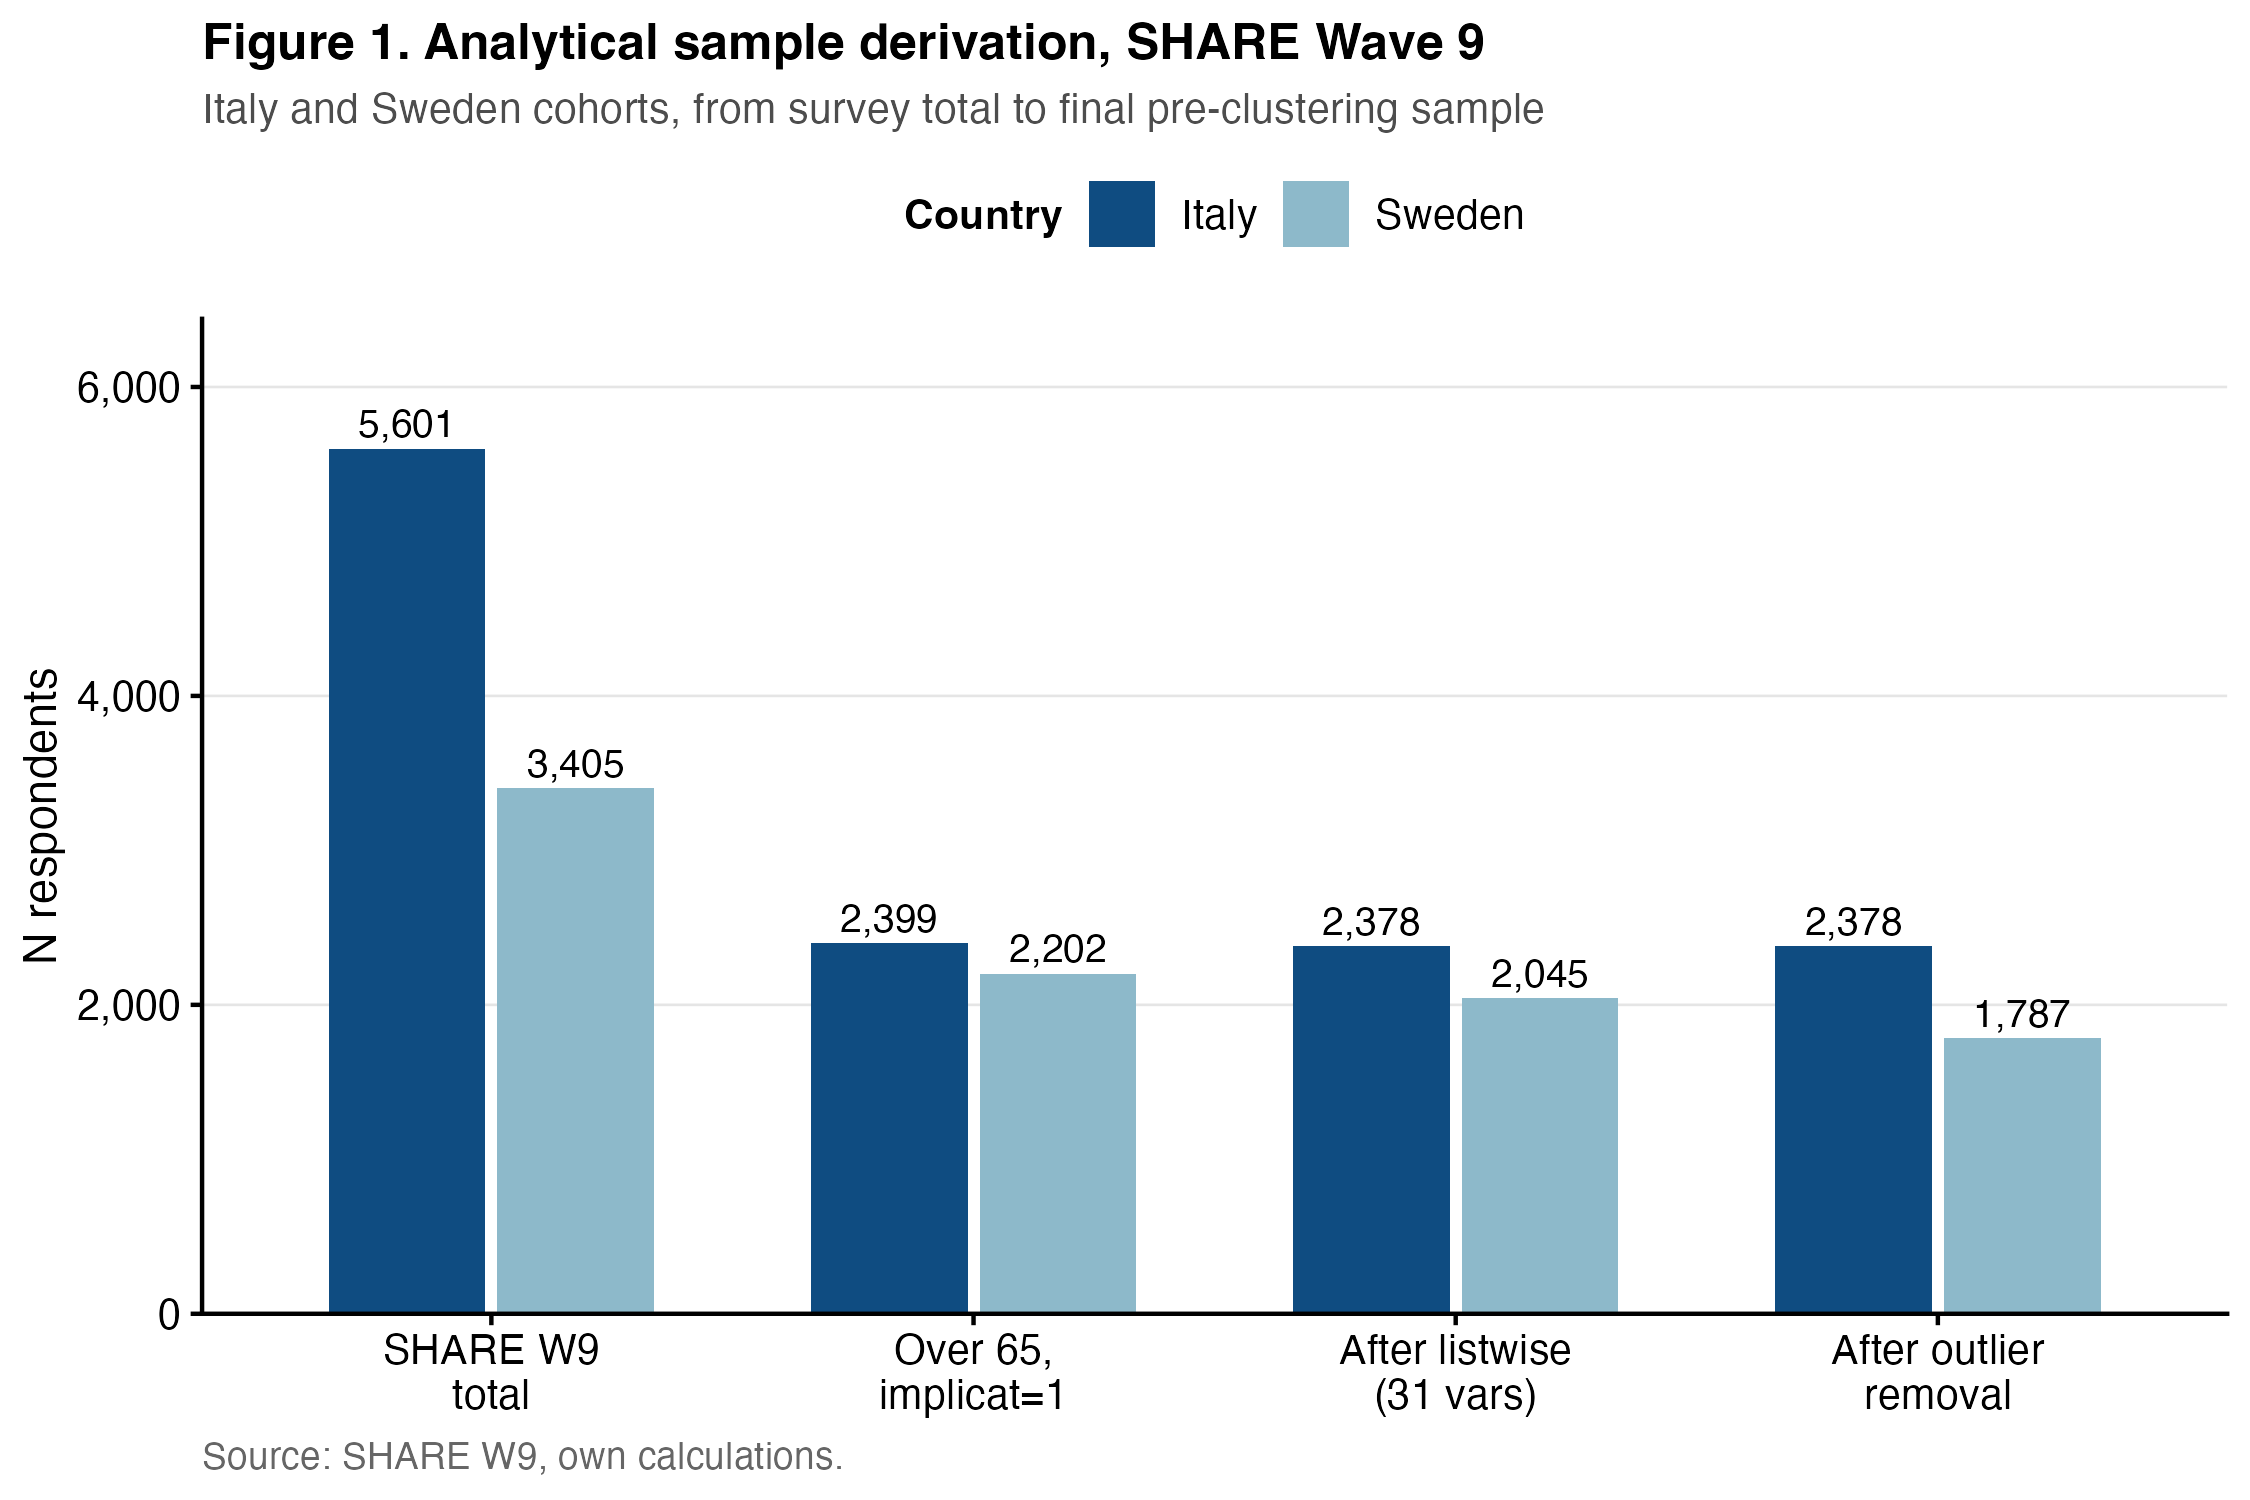
\includegraphics[width=0.85\linewidth]{figures/03_data_methods/fig_01_sample_flow.png}
  \caption{Analytical sample derivation, SHARE Wave 9. Italy and Sweden cohorts, from survey total to final pre-clustering sample. Source: SHARE W9, own calculations.}
  \label{fig:ch3-sample-flow}
\end{figure}

First, the analysis was limited to non-institutionalised respondents aged sixty-five years or older at the time of interview, retaining only the first implicate produced by SHARE's multiple-imputation procedure (\emph{implicat~==~1}). This restriction reduces the working samples to 2{,}399 (Italy) and 2{,}202 (Sweden) observations, consistent with the population of interest for research on ageing.

Second, complete-case listwise deletion was applied across the thirty-one analytical variables described in Section~\ref{sec:ch3-variables}. Listwise deletion, rather than multiple imputation, was chosen because the clustering and factor-analytic procedures at the centre of the analytical strategy require fully observed cases, and because the amount of missingness is modest and approximately missing-at-random on the selected items (Little \& Rubin, 2019). After this step the Italian sample stands at 2{,}378 respondents and the Swedish sample at 2{,}045.

Third, multivariate outliers were identified using the Mahalanobis distance against the correlation structure of the thirty-one standardised variables. A conservative $\chi^{2}$ cut-off at $p = 0.001$ (31 degrees of freedom) was adopted to avoid overly aggressive trimming. No Italian respondent exceeds the cut-off; 258 Swedish cases are flagged and removed. The final analytical samples are therefore $n = 2{,}378$ (Italy) and $n = 1{,}787$ (Sweden).

It should be noted that these final sample sizes differ from those reported in earlier iterations of the project design. This divergence reflects the adoption of a uniform, code-authoritative preprocessing pipeline that applies the same Mahalanobis threshold to both countries and does not rely on any previously computed cleaning artefacts. All empirical results presented in the remainder of the thesis derive from the samples described above.

\section{Variables}
\label{sec:ch3-variables}

The thirty-one analytical variables span five conceptual dimensions --- health, economic resources, digital and social engagement, cognitive function, and subjective well-being --- summarised in Table~\ref{tab:ch3-variables}. The selection replicates, within SHARE W9, the multidimensional structure of successful ageing proposed by Rowe and Kahn (1997), while incorporating the post-pandemic emphasis on digital inclusion that motivates much current research on ageing societies (Friemel, 2016; König et al., 2018).

\begin{table}[ht]
  \centering
  \caption{Analytical variables by conceptual dimension.}
  \label{tab:ch3-variables}
  \small
  \begin{tabular}{@{}lp{9.5cm}@{}}
    \toprule
    \textbf{Dimension} & \textbf{Variables}\\
    \midrule
    Health (8)               & \emph{sphus}, \emph{chronic}, \emph{adl}, \emph{iadl}, \emph{mobility}, \emph{eurod}, \emph{bmi}, \emph{phinact}\\
    Economic resources (5)   & \emph{log\_thinc}, \emph{log\_hnetw}, \emph{ypen1}, \emph{home\_own}, \emph{fdistress}\\
    Digital / social (10)    & \emph{internet}, \emph{ac035d1}, \emph{ac035d5}, \emph{ac035d8}, \emph{sp002\_}, \emph{sp008\_}, \emph{sn\_size\_w9}, \emph{social\_integration}, \emph{ac035d4}, \emph{ac035d7}\\
    Cognitive (3)            & \emph{fluency}, \emph{memory}, \emph{orienti}\\
    Subjective well-being (5)& \emph{loneliness}, \emph{casp}, \emph{hope\_future}, \emph{interest}, \emph{expect\_alive}\\
    \bottomrule
  \end{tabular}
  \par\smallskip
  \footnotesize \emph{Note.} Eleven variables are binary (\emph{phinact}, \emph{home\_own}, \emph{internet}, \emph{ac035d1}, \emph{ac035d5}, \emph{ac035d8}, \emph{sp002\_}, \emph{sp008\_}, \emph{ac035d4}, \emph{ac035d7}, \emph{hope\_future}); the remaining twenty are continuous or quasi-continuous. Short human-readable labels and measurement scales are given in Figures~4, 5, 34, 50, 51, 66 and~67; the full mapping is stored in the helper module \texttt{v9/var\_labels.R}.
\end{table}

Eleven of the thirty-one variables are binary (coded 0/1); twenty are continuous or quasi-continuous. Three SHARE items that might in principle have entered the analytical battery were excluded on grounds of cross-country comparability. The item \emph{pcskill\_r} (computer skills self-assessment) is administered only to respondents who report regular personal-computer use, yielding 48 per cent missing values in Sweden; the items \emph{wllft} and \emph{wllst} (immediate and delayed word recall) cover 22 and 25 per cent of the Swedish sample respectively, because they are administered only to a random sub-sample of participants. Retaining these items would have forced a much smaller common support, distorting the comparative exercise.

Two digital-engagement items require particular comment. In Italy, \emph{ac035d4} (participation in educational training) and \emph{ac035d7} (involvement in political organisations) have zero variance: no Italian respondent in the analytical sample reports either activity. This pattern appears to reflect an artefact of the Italian fieldwork rather than a substantive finding about participation, but it requires the two variables to be excluded from the Italian PCA and factor-analysis computations. In Sweden the same items exhibit low but non-zero variance (four to six per cent positive responses) and are therefore retained. The common analytical battery comprises twenty-nine active variables in Italy and thirty-one in Sweden; cross-country comparisons at the profile level rely on indicators that are active in both countries.

\section{Preprocessing}
\label{sec:ch3-preprocessing}

Two successive transformations were applied to the twenty non-binary variables prior to analysis, following the workflow established in the Bocconi course 20570 \emph{Data Analytics and Visualization} (Piccareta \& Trentini, 2025). First, each non-binary variable was rank-transformed using average-rank tie-breaking. Rank transformation uniformises marginal distributions and mitigates the influence of extreme values on the distance-based procedures that follow, at the cost of discarding information about absolute magnitudes. Second, every analytical variable --- binary and non-binary alike --- was standardised to zero mean and unit variance (z-score standardisation), so that no dimension dominates cluster formation or factor extraction by virtue of its original scale.

Binary variables were not rank-transformed, since the rank of a 0/1 variable collapses into a trivial two-valued distribution. They were nevertheless z-standardised jointly with the continuous variables, yielding a single homogeneous standardised matrix of thirty-one columns for Sweden and twenty-nine columns for Italy. This homogeneous standardised matrix is the direct input to the K-means, PCA, and factor-analysis procedures described below. For the Latent Class Analysis of Section~\ref{sec:ch3-lca}, the continuous variables are further discretised into tertiles, as detailed there.

\section{Analytical framework}
\label{sec:ch3-framework}

The empirical strategy of this thesis employs three complementary methods to produce and validate the multidimensional profiles of elderly Italians and Swedes. Each method rests on a different theoretical premise and draws on a different statistical tradition, and their triangulation serves to evaluate whether a given profile reflects a robust population type or a method-specific artefact (Magidson \& Vermunt, 2002).

\subsection{Dimension-wise Principal Component Analysis}
\label{sec:ch3-pca}

Principal Component Analysis (PCA) was applied separately to each of the five conceptual dimensions. This dimension-wise decomposition serves three purposes: it summarises the correlational structure of the three to ten indicators within each dimension into a smaller set of orthogonal components; it provides diagnostics for the presence of a natural latent structure within each domain; and it anchors the downstream outlier analysis that flagged Swedish extreme respondents.

Components were retained on the basis of Kaiser's criterion (eigenvalue greater than one), with one documented exception. For the digital/social block, four components were retained in both countries even though the fourth component has an eigenvalue just below unity (0.96 in Italy, 0.98 in Sweden). Two considerations motivated this departure. First, when Kaiser's threshold lies so near one, the criterion provides only weak guidance. Second, the fourth component carries meaningful substantive content --- it captures a latent axis of civic and political engagement independent of generic digital use --- and the ensuing outlier diagnostics depend on it to flag extreme respondents. Retaining four components therefore maximises comparability with the reference design and ensures that the cross-country profile structures remain commensurable.

\subsection{Factor analysis}
\label{sec:ch3-fa}

A second lens on the variable space is provided by exploratory factor analysis, fitted with principal-axis extraction, varimax rotation, and six factors per country. Factor analysis differs from PCA in two respects: it isolates the shared-variance component of each indicator, discarding uniquenesses, and it rotates the latent space to approximate simple structure (each indicator loading primarily on one factor). The course treats factor analysis as the preferred tool for substantive interpretation of latent constructs (Piccareta \& Trentini, 2025), while reserving PCA for dimensionality reduction.

The six-factor solution is justified \emph{ex ante} by theoretical expectations --- five substantive dimensions plus a mood-versus-cognition distinction within the subjective block --- and \emph{ex post} by empirical diagnostics. The Kaiser--Meyer--Olkin measure of sampling adequacy equals 0.832 in Italy and 0.808 in Sweden, both above the meritorious threshold (Kaiser \& Rice, 1974). Bartlett's test of sphericity is rejected at any conventional level in both countries ($\chi^{2} = 18{,}755$, $df = 406$ for Italy; $\chi^{2} = 9{,}067$, $df = 465$ for Sweden; both $p < 10^{-300}$). Parallel analysis with one hundred random datasets suggests ten factors in Italy and nine in Sweden; Kaiser's criterion on the full correlation matrix indicates nine and ten respectively. The six-factor solution is therefore conservative and is retained on interpretive grounds and for cross-country comparability, with the BIC-minimal larger solutions reported as sensitivity analyses in Chapter~6.

One diagnostic deserves explicit mention: in Sweden, \emph{social\_integration} exhibits a Heywood case with an estimated loading of 1.11 on its dominant factor, yielding a communality of 1.38 once small secondary loadings are added in quadrature. This pattern reflects the near-perfect determination of the social-integration index by its dominant factor; it is flagged rather than treated. Chapter~6 discusses its implications for the stability of the Swedish solution and evaluates alternative parameterisations.

\subsection{K-means clustering}
\label{sec:ch3-kmeans}

The core segmentation device of this thesis is K-means clustering, applied to the thirty-one (respectively twenty-nine) standardised variables rather than to any factor- or component-derived score. This choice follows the methodological guidance of course 20570 (Piccareta \& Trentini, 2025) and ensures that profile means can be interpreted directly in the metric of the original indicators. Clustering on factor scores is sometimes preferred in the literature on latent-variable segmentation (Magidson \& Vermunt, 2002), but it complicates the interpretation of profile characteristics and, as shown in Chapter~6, may produce unstable assignments when the factor solution itself contains Heywood cases.

For each country, K-means was initialised with one hundred random restarts, a maximum of five hundred iterations per restart, and a fixed random seed (42) for reproducibility. The number of clusters was fixed at six for both countries at the model-fitting stage, consistent with the reference design. In Italy, the six-cluster solution was subsequently refined by removing any micro-cluster smaller than five per cent of the sample and characterised by extreme digital-component scores; at $n = 2{,}378$ no such micro-cluster emerged, and the analysis was refitted directly with $k = 5$ on the full sample. In Sweden the six-cluster solution was retained without further removal, since no micro-cluster emerged --- a pattern that is consistent with the reference design's observation that the Italian micro-cluster has no Swedish analogue.

K-means was preferred over hierarchical alternatives on empirical grounds. The within-cluster quality indexes computed across $k = 2,\ldots,12$ show that K-means attains uniformly higher within-cluster $R^{2}$ and silhouette than Ward, complete, and average linkage in both countries; Ward only rivals K-means on the Dunn index, which penalises cluster elongation differently. This comparison is summarised in Figures~22--23 (K-means diagnostics by country) and in the multi-algorithm overlay of Figures~64--65, which presents all six indexes ($R^{2}$, Pseudo-F, silhouette, Davies-Bouldin proxy, Dunn and Pearson--gamma) for the four algorithms on a common scale. Figures~66--67 further document, variable by variable, how the within-cluster $R^{2}$ saturates with $k$ for each algorithm, highlighting a small group of indicators (e.g.\ body mass index, received help) that carry no clustering signal under any method and a larger group whose separation stabilises precisely in the $k = 5,\ldots,6$ range.

The choice of $k = 5$ for Italy and $k = 6$ for Sweden rests on three converging criteria. First, the silhouette and $R^{2}$ curves of Figures~22--23 flatten beyond these values, indicating diminishing returns from further partitioning. Second, the semi-partial $R^{2}$ and Pseudo-$T^{2}$ (Duda--Hart) diagnostics reported in the appendix (Figures~72--73) display the sharpest merge-cost jumps when $k$ crosses the chosen cut-off, consistent with a natural boundary in the dendrogram. Third, the five- and six-cluster solutions produce substantively interpretable profiles that map onto the welfare-regime hypotheses of Chapter~5; solutions with $k > 6$ split the Connected and Social profiles into thematically redundant fragments, while $k < 5$ collapses the Fragile Resigned / Fragile Depressed contrast that is the analytical payoff of the subjective-wellbeing block.

\subsection{Latent Class Analysis}
\label{sec:ch3-lca}

A third, probabilistic lens on the same population is provided by Latent Class Analysis (LCA), fitted using the R package \emph{poLCA} (Linzer \& Lewis, 2011). LCA models the joint distribution of categorical indicators as a mixture of latent-class-specific multinomial distributions, yielding a fully probabilistic assignment of respondents to classes. Whereas K-means imposes hard, distance-based partitions, LCA produces posterior probabilities over all latent classes for every individual and thus supports a more explicit assessment of classification uncertainty (Collins \& Lanza, 2010).

\emph{poLCA} requires categorical indicators, so the twenty non-binary variables were discretised into tertiles (1 = low, 2 = mid, 3 = high) prior to fitting. Five variables whose distributions are heavily zero-inflated --- \emph{adl}, \emph{iadl}, \emph{memory}, \emph{orienti} and \emph{interest} --- admit only two or two-plus-one effective categories; for these a mode-based split was adopted (one category for the modal value, one or two for the remainder). For each country, LCA was estimated for $k = 2$ through $k = 8$ with five random restarts and up to one thousand EM iterations per fit. Normalised entropy (computed from the posterior matrix) and the Bayesian Information Criterion are reported for all fits. Chapter~6 uses these criteria, alongside the cluster-level convergence between K-means and LCA assignments, to evaluate the robustness of the segmentation.

\section{Validation strategy}
\label{sec:ch3-validation}

Three complementary validation strategies are used throughout the thesis.

First, external validation exploits a variable that did not enter the clustering. Life satisfaction --- measured on the SHARE zero-to-ten scale (\emph{ac012\_}) and absent from the analytical battery --- is regressed on the profile factor through a one-way analysis of variance (ANOVA) in each country. A strong between-group effect indicates that the profiles capture real variation in aspects of well-being that were not used in their construction. Welch's $t$-test and Tukey's HSD are used for post-hoc pairwise comparisons and adjust for unequal variances and multiplicity.

Second, internal consistency is assessed by comparing K-means and LCA assignments on the same individuals. A cluster-specific convergence rate is computed as the share of members of a given K-means profile that are also assigned to the modal LCA class. High convergence indicates a robust latent type, while low convergence flags a profile that is geometrically well-defined but probabilistically ambiguous.

Third, cross-country comparability is evaluated through four matched profile pairs constructed to correspond semantically across Italy and Sweden, as detailed in Table~\ref{tab:ch3-matched-pairs}. Welch's $t$-tests compare the Italian and Swedish members of each pair on the core well-being and connectedness variables, and chi-squared tests perform the analogous comparison on binary indicators. Profiles that have no cross-country analogue are reported separately as welfare-regime-specific types and listed in the bottom row of Table~\ref{tab:ch3-matched-pairs}.

\begin{table}[ht]
  \centering
  \caption{Cross-country matched-pair mapping between Italian and Swedish profiles.}
  \label{tab:ch3-matched-pairs}
  \small
  \begin{tabular}{@{}lll@{}}
    \toprule
    \textbf{Matched pair} & \textbf{Italian profile} & \textbf{Swedish profile}\\
    \midrule
    Fragile            & \emph{Fragile Resigned}   & \emph{Fragile}\\
    Declining          & \emph{Fragile Depressed}  & \emph{Social Decline}\\
    Socially-oriented  & \emph{Traditional Social} & \emph{Moderate}\\
    Connected          & \emph{Connected Active}   & \emph{Connected Wealthy}\\
    \midrule
    Unmatched          & \emph{Moderate Isolated}  & \emph{Asset Rich}, \emph{Wealthy Digital}\\
    \bottomrule
  \end{tabular}
  \par\smallskip
  \footnotesize \emph{Note.} Profiles in the first four rows are compared on well-being and connectedness variables via Welch's $t$-tests and chi-squared tests. Profiles in the bottom row have no cross-country analogue and are reported as welfare-regime-specific types in Chapter~5.
\end{table}

\section{Software and reproducibility}
\label{sec:ch3-software}

All analyses were conducted in R 4.5 (R Core Team, 2024) with the following principal packages: \emph{psych} 2.3 (factor analysis and KMO/Bartlett diagnostics), \emph{cluster} 2.1 (silhouette computation), \emph{poLCA} 1.6 (latent class analysis), \emph{haven} 2.5 (reading SHARE Stata files), and the \emph{tidyverse} suite (data manipulation and visualisation). The analytical pipeline is organised into twenty numbered R scripts --- from raw SHARE file ingestion to final figure generation --- together with two shared helper modules: a central variable-label dictionary (\texttt{v9/var\_labels.R}) and a chapter-routing utility (\texttt{v9/fig\_paths.R}) that deposits each figure under the appropriate chapter subfolder. All twenty-two files are available in the online appendix. Each script uses a fixed random seed (42) wherever stochasticity is involved; the total execution time from raw files to final figures is approximately forty minutes on a standard laptop, with the cluster-diagnostic scripts (hierarchical linkages over $k = 2,\ldots,12$) accounting for the bulk of the runtime.

Raw SHARE data are used under the conditions of Release 9.0.0, which require an end-user licence and prohibit disclosure of individual-level data. All aggregate results and figures presented in this thesis comply with the SHARE publication guidelines; no individual respondent is identifiable from the results reported.

\chaptertitlepage{The Italian Typology}{Five archetypes of late-life experience in Italy}
\label{ch:ch4}

\section{Overview}
\label{sec:ch4-overview}

This chapter presents the five-archetype typology of the Italian over-65 population recovered from the K-means segmentation of Chapter~3. \S\ref{sec:ch4-five-archetypes} reports the population-level structure of the partition. \S\ref{sec:ch4-profile-descriptions} describes the five archetypes profile by profile. \S\ref{sec:ch4-integrative-view} presents the integrative profile fingerprint. \S\ref{sec:ch4-external-validation} reports external validation against life satisfaction. \S\ref{sec:ch4-demographics} reports the demographic composition by gender and age band. \S\ref{sec:ch4-isolation-paradox} develops the Isolation Paradox --- the most distinctive and policy-relevant finding of the Italian typology. \S\ref{sec:ch4-synthesis} closes with synthesis.

All centroid coordinates are reported as z-scores within Italy on the analytical sample ($n = 2{,}378$). The substantive direction of each variable is reported in parenthesis at first mention. National projection uses the Istat 2024 estimate of 14.18 million Italian residents aged 65 or older.

\section{The five archetypes}
\label{sec:ch4-five-archetypes}

The K-means segmentation with $k = 5$ partitions the 2,378 Italian respondents into five clusters. Figure~\ref{fig:ch4-profiles} reports cluster mean values on eight diagnostic variables, with profiles ordered from most fragile (left) to most connected (right). Table~\ref{tab:ch4-archetypes} lists the archetypes with their headline signature and population shares.

\begin{figure}[ht]
  \centering
  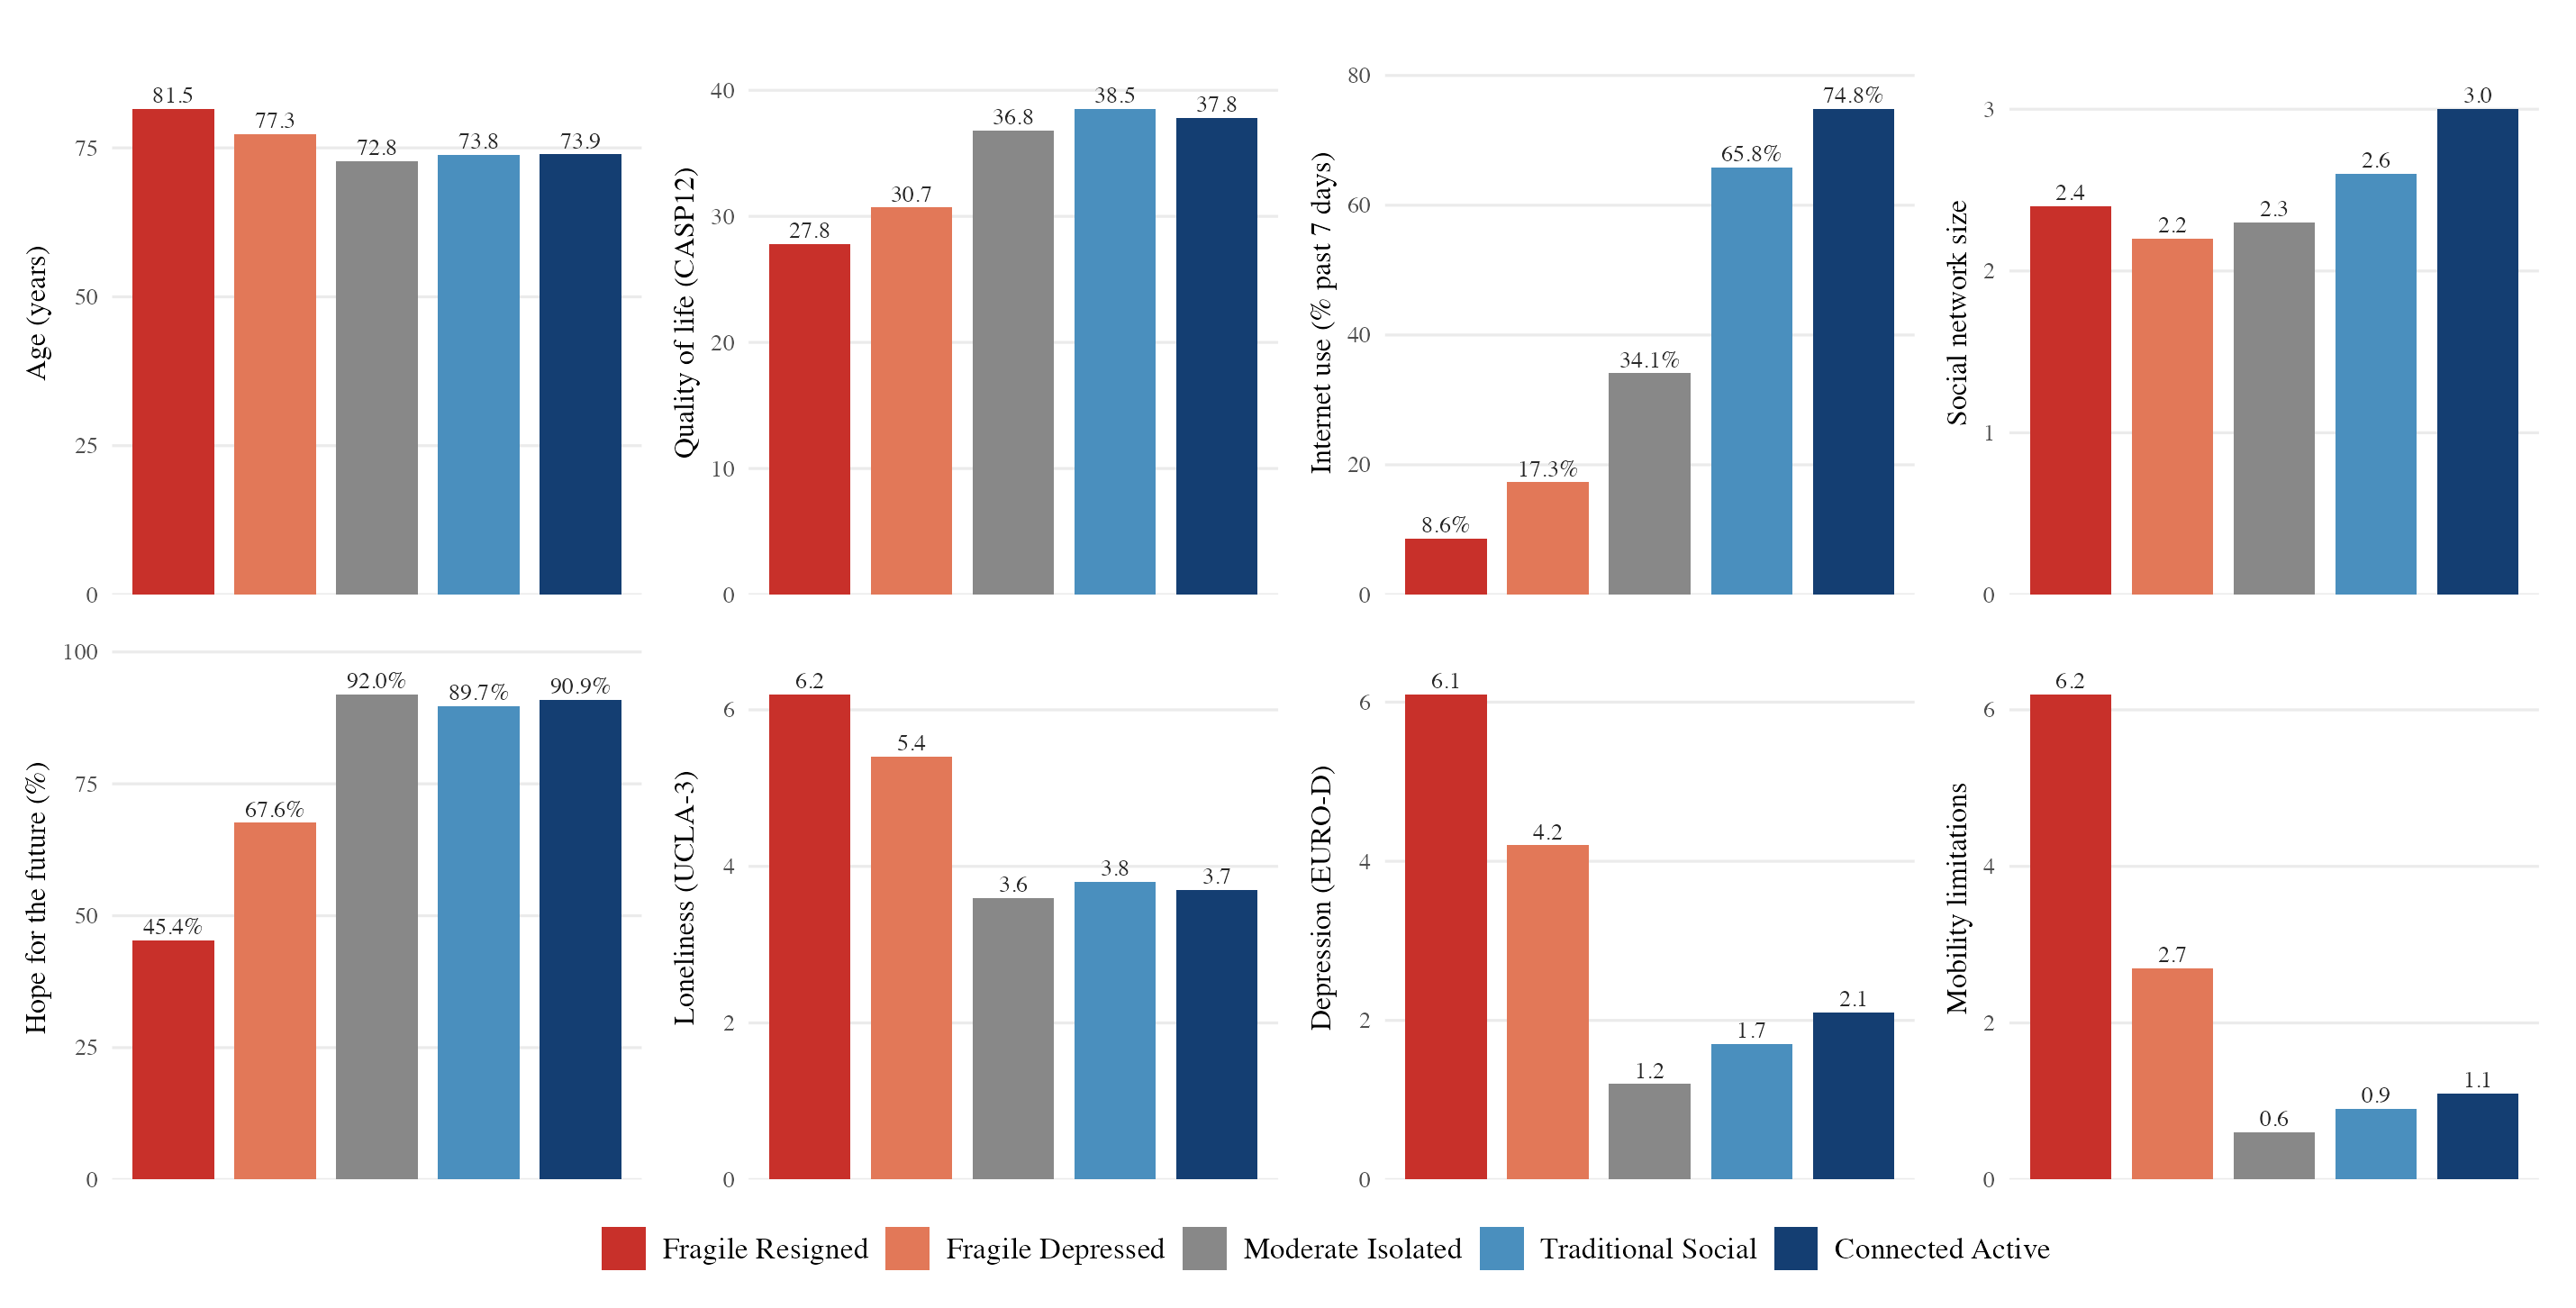
\includegraphics[width=0.95\linewidth]{figures/04_italy/fig_4_1_NEW.png}
  \caption{Profile characteristics, Italy. Mean values for each of the five archetypes on eight key dimensions: age, CASP-12 (12--48), internet (\% in past seven days), loneliness (UCLA-3, higher = lonelier), hope for the future (\% reporting hopes), social-network size, EURO-D depression (higher = more depressive symptoms), mobility limitations. Profiles ordered from most fragile to most connected. $N = 2{,}378$.}
  \label{fig:ch4-profiles}
\end{figure}

\begin{table}[ht]
  \centering
  \caption{Headline signature of the five Italian archetypes}
  \label{tab:ch4-archetypes}
  \begin{tabular}{p{2.5cm}p{1.2cm}p{7cm}}
    \toprule
    \textbf{Archetype} & \textbf{Share} & \textbf{Headline signature} \\
    \midrule
    Fragile Resigned & 14.4\% & Worst health, oldest age (mean 81.5 yr), lowest internet use (8.6\%) and CASP (27.8). Sub-clinical depression (EURO-D 6.1). Withdrawn evaluative orientation (hope 45.4\%). \\
    Fragile Depressed & 11.7\% & Persistent depressive affect (EURO-D 4.2, loneliness 5.4) with intermediate functional health and below-average resources. \\
    Moderate Isolated & 28.1\% & Average to good health (mobility 0.6, EURO-D 1.2) and resources, but restricted social engagement (network 2.3, internet 34.1\%). The largest single archetype and the country-specific Italian configuration. \\
    Traditional Social & 25.1\% & Good health and resources, dense cultural participation (hope 89.7\%), moderate internet adoption (65.8\%). Highest CASP (38.5). \\
    Connected Active & 20.7\% & Highest digital adoption (74.8\%), largest network (3.0), best resources, intact health. CASP 37.8. The silver-economy frontier of the Italian over-65 population. \\
    \bottomrule
  \end{tabular}
\end{table}

\noindent\small Note. Headline values are raw means of the diagnostic variables of Figure~\ref{fig:ch4-profiles}. Standardised centroid coordinates are reported in \S\ref{sec:ch4-profile-descriptions}. \normalsize

Two raw-scale observations from Figure~\ref{fig:ch4-profiles} anchor the standardised description that follows. First, the age gradient: the Fragile Resigned cluster has a mean age of 81.5 years, against 77.3 (Fragile Depressed), 72.8 (Moderate Isolated), 73.8 (Traditional Social) and 73.9 (Connected Active). The Fragile Resigned are on average eight years older than the four other archetypes, identifying the oldest-old segment of the population. Second, the digital divide: 8.6\% in Fragile Resigned versus 74.8\% in Connected Active --- a near nine-fold gap on a single behavioural indicator. From the silver-economy perspective, this gap defines the boundary between sub-populations served by digital products and those for whom traditional welfare and family-based provision remain the only operational channel.

\section{Profile descriptions}
\label{sec:ch4-profile-descriptions}

\subsection{Fragile Resigned}
\label{sec:ch4-fragile-resigned}

The Fragile Resigned cluster accounts for 14.4\% of the Italian over-65 population ($\approx 2.04$ million individuals). It sits at the most adverse end of every health dimension: self-rated health $+1.06$ (higher = worse), IADL $+1.97$, mobility $+1.38$, ADL $+1.74$, chronic conditions $+0.85$, EURO-D $+1.04$, physical inactivity $+1.05$. Mean age is 81.5 years --- eight years above the typology average --- identifying the oldest-old segment. Economic resources are below the Italian mean (log\_thinc $-0.19$, log\_hnetw $-0.34$) but the gap is small in standardised terms; the principal axis of fragility is health and functional autonomy, not income.

The subjective signature is the lowest in the typology on every evaluative dimension. CASP-12 is at $-1.02$ (raw 27.8), hope for the future at $-0.82$ (45.4\% report hopes, against $\geq 90\%$ in non-fragile profiles), interest at $-0.50$, expected survival at $-0.59$, loneliness at $+0.88$. The combination --- high subjective burden, low evaluative function, low expectation --- supports the descriptive label ``Resigned'': a cluster evaluatively withdrawn, with a configuration consistent with chronic adaptation to the constraints of advanced old age. Cognitive deficits are pronounced (orienti $-1.00$, fluency $-0.75$). The cluster is the principal target of the Italian long-term-care welfare branch and identifies the lower bound of the silver-economy market: a sub-population whose digital and behavioural channels are essentially closed and whose service consumption is mediated by family caregivers and institutional providers \citep{ferrera1996, saraceno2010}.

\subsection{Fragile Depressed}
\label{sec:ch4-fragile-depressed}

The Fragile Depressed cluster accounts for 11.7\% ($\approx 1.66$ million). It is intermediate on objective health and functional dimensions (sphus $+0.47$, EURO-D $+0.54$ with raw mean 4.2 just above the four-point clinical threshold, mobility $+0.36$, chronic conditions $+0.32$). Mean age is 77.3 years. Economic resources are below the Italian mean (log\_thinc $-0.39$, log\_hnetw $-0.40$, fdistress $-0.51$). The subjective signature is the second-lowest in the typology but qualitatively different from Fragile Resigned: CASP $-0.67$ (raw 30.7), loneliness $+0.59$ (raw 5.4), hope $-0.28$ (67.6\% report hopes --- clearly above 45.4\% of Fragile Resigned but below the non-fragile profiles). The cluster displays elevated depressive affect and loneliness without the same magnitude of withdrawal from hope and interest --- an active depressive episode rather than a settled withdrawal.

The contrast with Fragile Resigned is among the most substantively important findings of the Italian typology and one of the principal arguments for retaining $k = 5$ over $k = 4$ (Chapter~3). Demographically, the cluster is over-represented among Italian women: 31\% of women fall in Fragile Depressed against 22\% of men (\S\ref{sec:ch4-demographics}). Internet use is 17.3\% --- non-trivial but well below the non-fragile profiles. From the silver-economy perspective, the Fragile Depressed represent a configuration in which behavioural and digital channels remain partially open but the affective barrier is the binding constraint on adoption.

\subsection{Moderate Isolated}
\label{sec:ch4-moderate-isolated}

The Moderate Isolated cluster is the largest, at 28.1\% of the over-65 population ($\approx 3.98$ million individuals). The cluster sits at or near the Italian mean on most objective health and resource dimensions: sphus $-0.58$ (better than mean), EURO-D $-0.68$ (raw 1.2, well below the clinical threshold), mobility $-0.61$, IADL $-0.42$, log\_thinc $-0.33$, log\_hnetw $-0.22$, fdistress $-0.16$. Mean age is 72.8 years (the youngest of the five archetypes). The cluster is not characterised by adversity on health or economic dimensions: it is, in absolute terms, an averagely-resourced and averagely-healthy segment.

The diagnostic feature is the position on social, cultural and digital dimensions: network size $-0.22$ (raw 2.3 confidants), social\_integration $-0.11$, internet $-0.11$ (raw 34.1\%), three cultural-engagement indicators between $-0.15$ and $-0.37$, provision of help to grandchildren $-0.15$. None of these distances is large in absolute terms, but the joint pattern across the social and cultural variables identifies a configuration in which the social and informational ecosystem is materially thinner than in the rest of the typology. The cluster does not report itself as particularly lonely (loneliness raw 3.6, well below the Italian mean), despite the thin network --- consistent with the observation that loneliness in older age is less a function of absolute network size than of the discrepancy between desired and actual configuration \citep{hawkleycacioppo2010}.

The Moderate Isolated archetype is the most distinctive feature of the Italian typology and does not have a structural counterpart in the Swedish typology of Chapter~5. The substantive interpretation, developed in Chapter~6, is that this configuration reflects the Mediterranean familistic regime: a substantial fraction of the Italian middle stratum is socially anchored to the immediate family and the residential neighbourhood, with limited participation in the kinds of associational and cultural activities that the Swedish welfare state and civil society make available to comparable individuals. The behavioural and policy consequences --- including the under-utilisation of healthcare relative to Traditional Social peers --- are developed in \S\ref{sec:ch4-isolation-paradox} as the Isolation Paradox.

\subsection{Traditional Social}
\label{sec:ch4-traditional-social}

The Traditional Social cluster accounts for 25.1\% ($\approx 3.56$ million). It sits in the upper region of the resource and health distributions (sphus $-0.40$, IADL $-0.42$, log\_thinc $+0.41$, log\_hnetw $+0.55$, fdistress $+0.43$; mean age 73.8 years), in a comparable position to the Connected Active. The diagnostic feature is the configuration of social, cultural and digital engagement: the centroid is at $+3.29$ standard deviations on the cultural-engagement indicator ac035d5, $+0.43$ on ac035d1, $+0.50$ on educational participation (ac035d8), $+0.50$ on provision of help to grandchildren (sp008\_), $+0.62$ on social integration. Internet use is at $+0.53$ (raw 65.8\%) --- well above the Italian mean but materially below Connected Active (74.8\%).

The cluster is the carrier of a dense and traditional pattern of social and cultural participation: institutionalised cultural attendance, organised volunteering, intergenerational support, and a moderate digital engagement that complements rather than substitutes for offline activities. CASP-12 is the highest in the typology (raw 38.5, $z = +0.66$), loneliness is low ($z = -0.39$), hope is positive (89.7\%). From the silver-economy perspective, the cluster is the segment most receptive to hybrid product designs that combine digital interfaces with offline community channels (parish-based or club-based intermediation of digital services), while the Connected Active cluster supports direct-to-consumer digital products without intermediation.

\subsection{Connected Active}
\label{sec:ch4-connected-active}

The Connected Active cluster accounts for 20.7\% ($\approx 2.94$ million). It sits at the high-resource end of the typology on every economic dimension (log\_thinc $+0.72$, log\_hnetw $+0.64$, ypen1 $+0.53$, home\_own $+0.24$, fdistress $+0.68$) and on every health dimension (sphus $-0.28$, EURO-D $-0.25$, mobility $-0.30$, chronic $-0.12$). Mean age is 73.9 years. The diagnostic feature is digital integration and informational engagement: internet use at $+0.72$ (raw 74.8\%, the highest in the Italian typology), educational participation at $+0.74$, verbal fluency at $+0.63$ (the highest cognitive score), network size at $+0.42$ (raw 3.0, the highest). The configuration is the ``successful aging'' pattern of the gerontological literature \citep{rowekahn1997} operationalised on a contemporary Italian sample. CASP-12 is high (raw 37.8, $z = +0.56$), loneliness is low (raw 3.7), hope is at 90.9\%, expected survival at $+0.18$.

The Connected Active cluster maps onto the Swedish Connected Wealthy archetype with broadly similar standardised positions, but represents a smaller share (20.7\% vs 29.5\% in Sweden (Connected Wealthy archetype) --- Chapter~6). From the silver-economy perspective, the cluster constitutes the immediate and ready-to-serve market for digital products and services targeted at older adults in Italy: 2.94 million individuals with high digital adoption, high economic resources, and intact health. Together with Traditional Social (3.56 million, partially digitally engaged), the Connected Active cluster defines the upper bound of the Italian silver-economy addressable market under current technology-adoption conditions.

\section{Integrative view: the typology fingerprint}
\label{sec:ch4-integrative-view}

The five-archetype centroid configuration is visualised in two complementary forms. Figure~\ref{fig:ch4-fingerprint} reports the profile fingerprint as a faceted view, with one panel per archetype showing the standardised mean across the 29 active variables; variables are grouped by dominant Factor Analysis loading (Chapter~3). Figure~\ref{fig:ch4-fa-scatter} plots all Italian respondents on the FA1 $\times$ FA2 plane (FA1: physical and functional fragility; FA2: high values correspond to worse subjective wellbeing), with diamonds marking cluster centroids and ellipses marking 50\% confidence regions per profile.

\begin{figure}[ht]
  \centering
  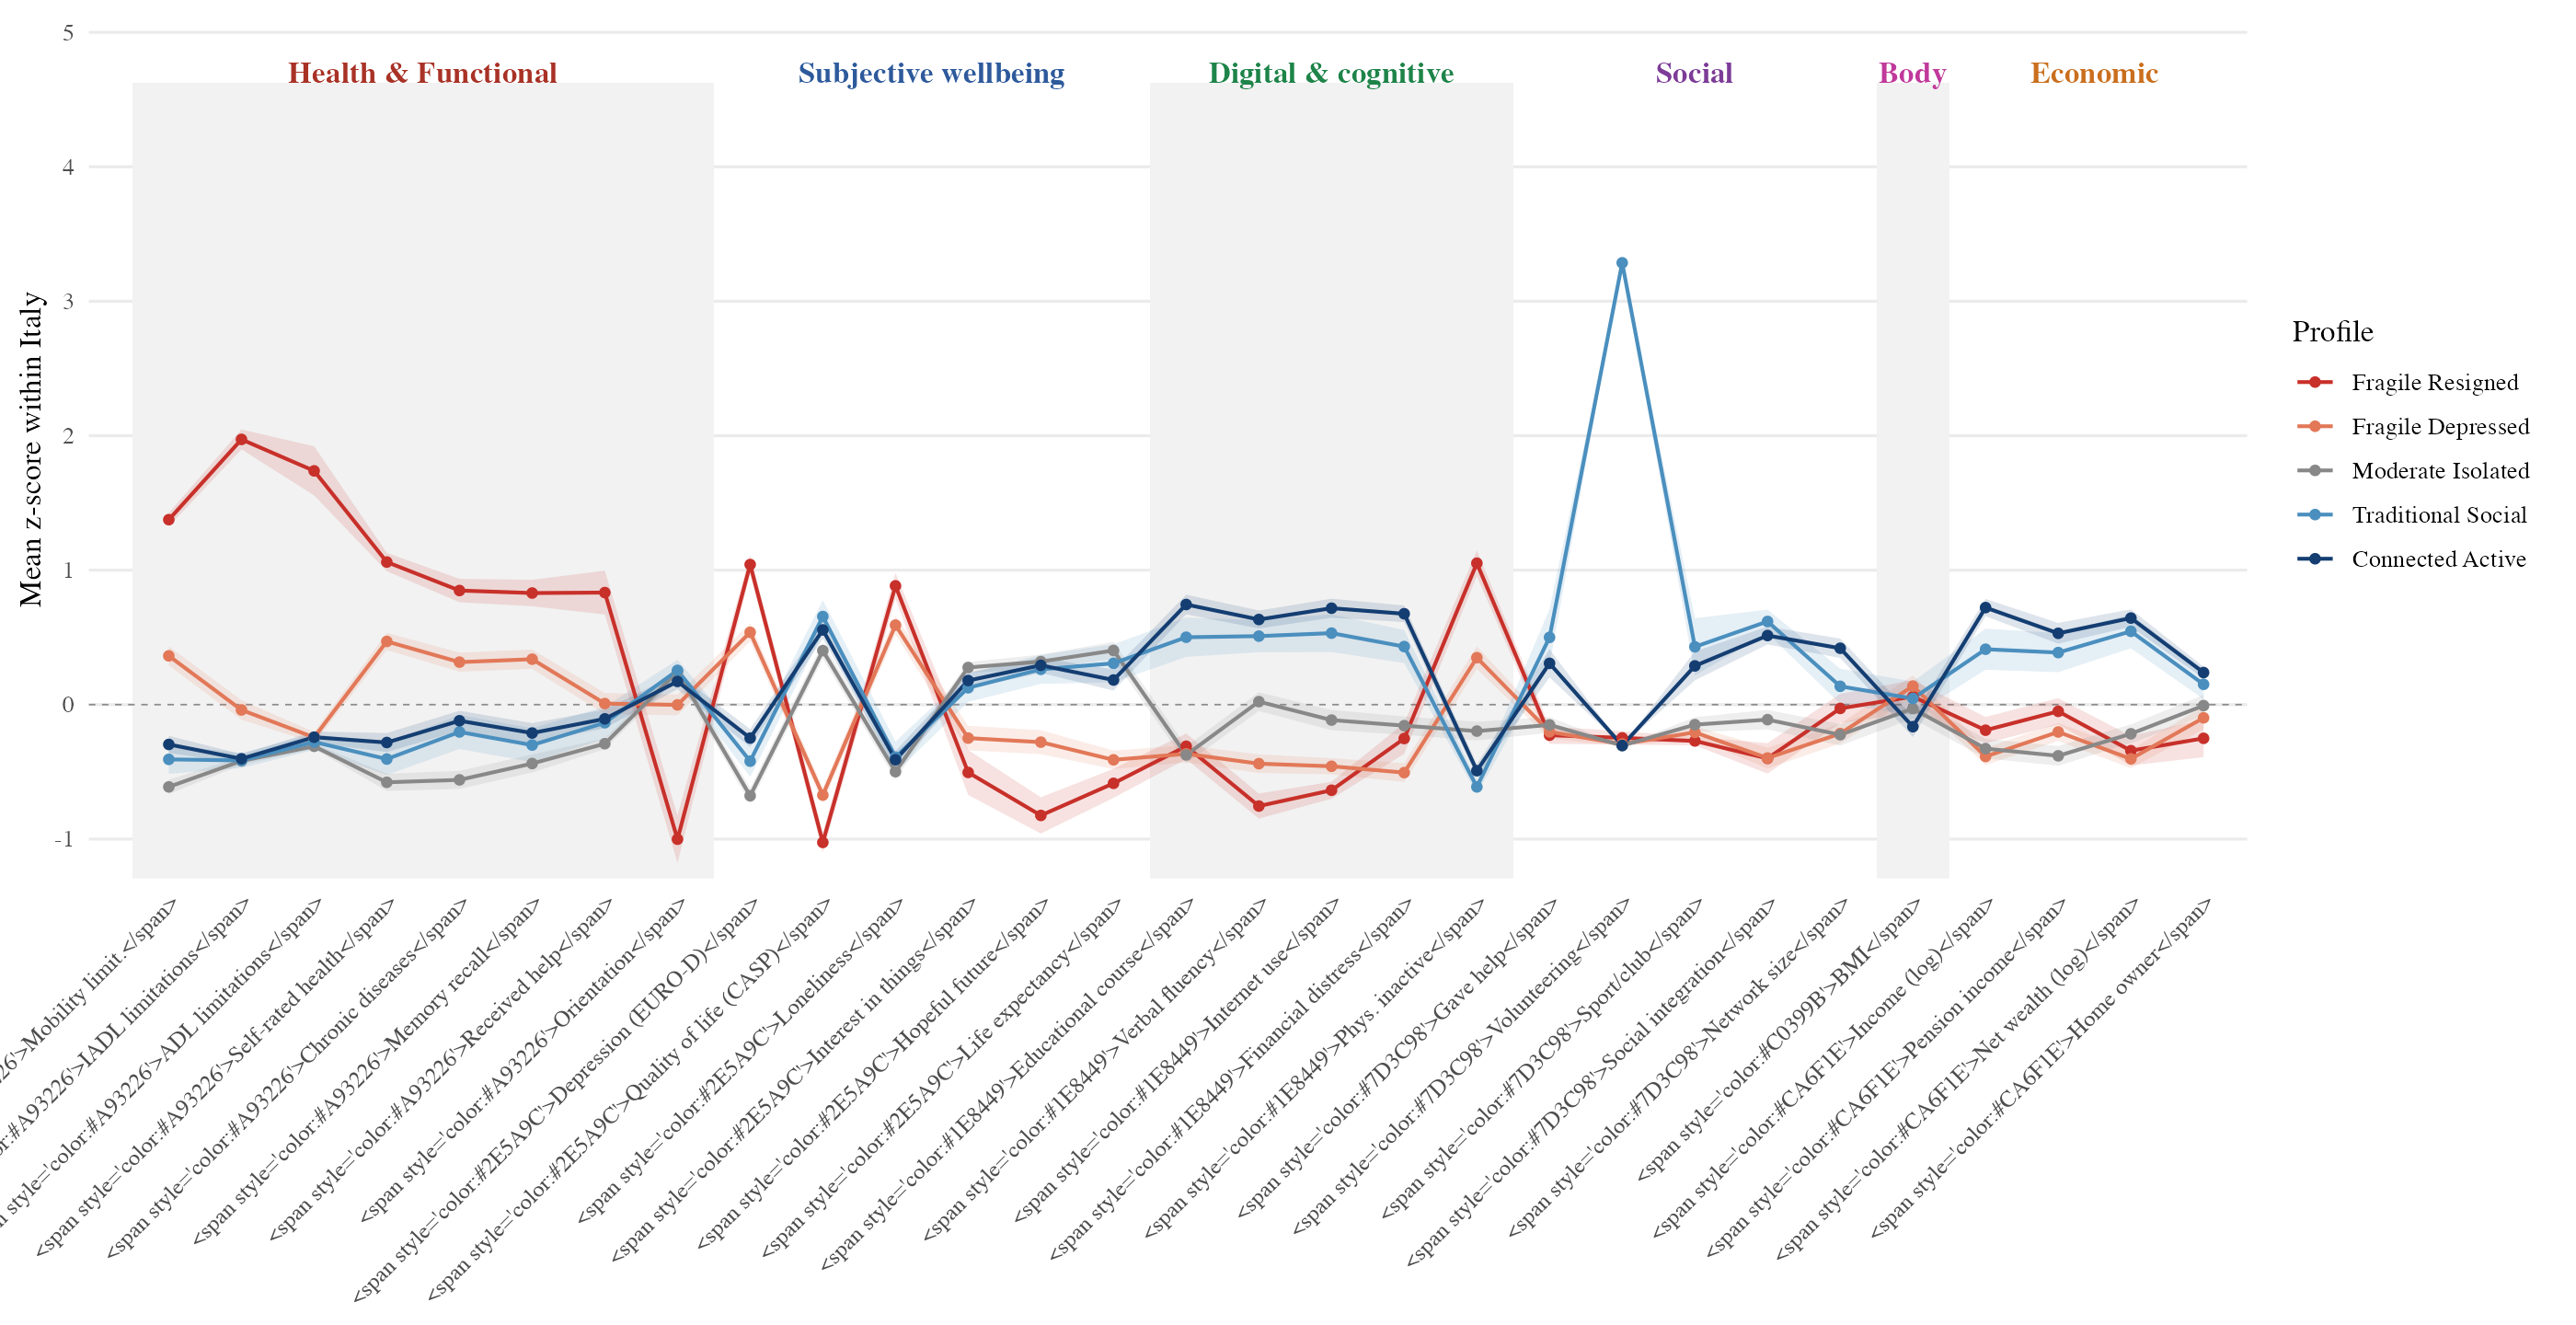
\includegraphics[width=0.95\linewidth]{figures/04_italy/fig_fingerprint_facet_italy.png}
  \caption{Profile fingerprint, Italy. Mean z-score per profile across the 29 active analytical variables, with 95\% bootstrap confidence ribbons ($n = 2{,}378$). Variables grouped by dominant Factor Analysis loading and ordered within factor; x-axis labels colour-coded by dimension.}
  \label{fig:ch4-fingerprint}
\end{figure}

\begin{figure}[ht]
  \centering
  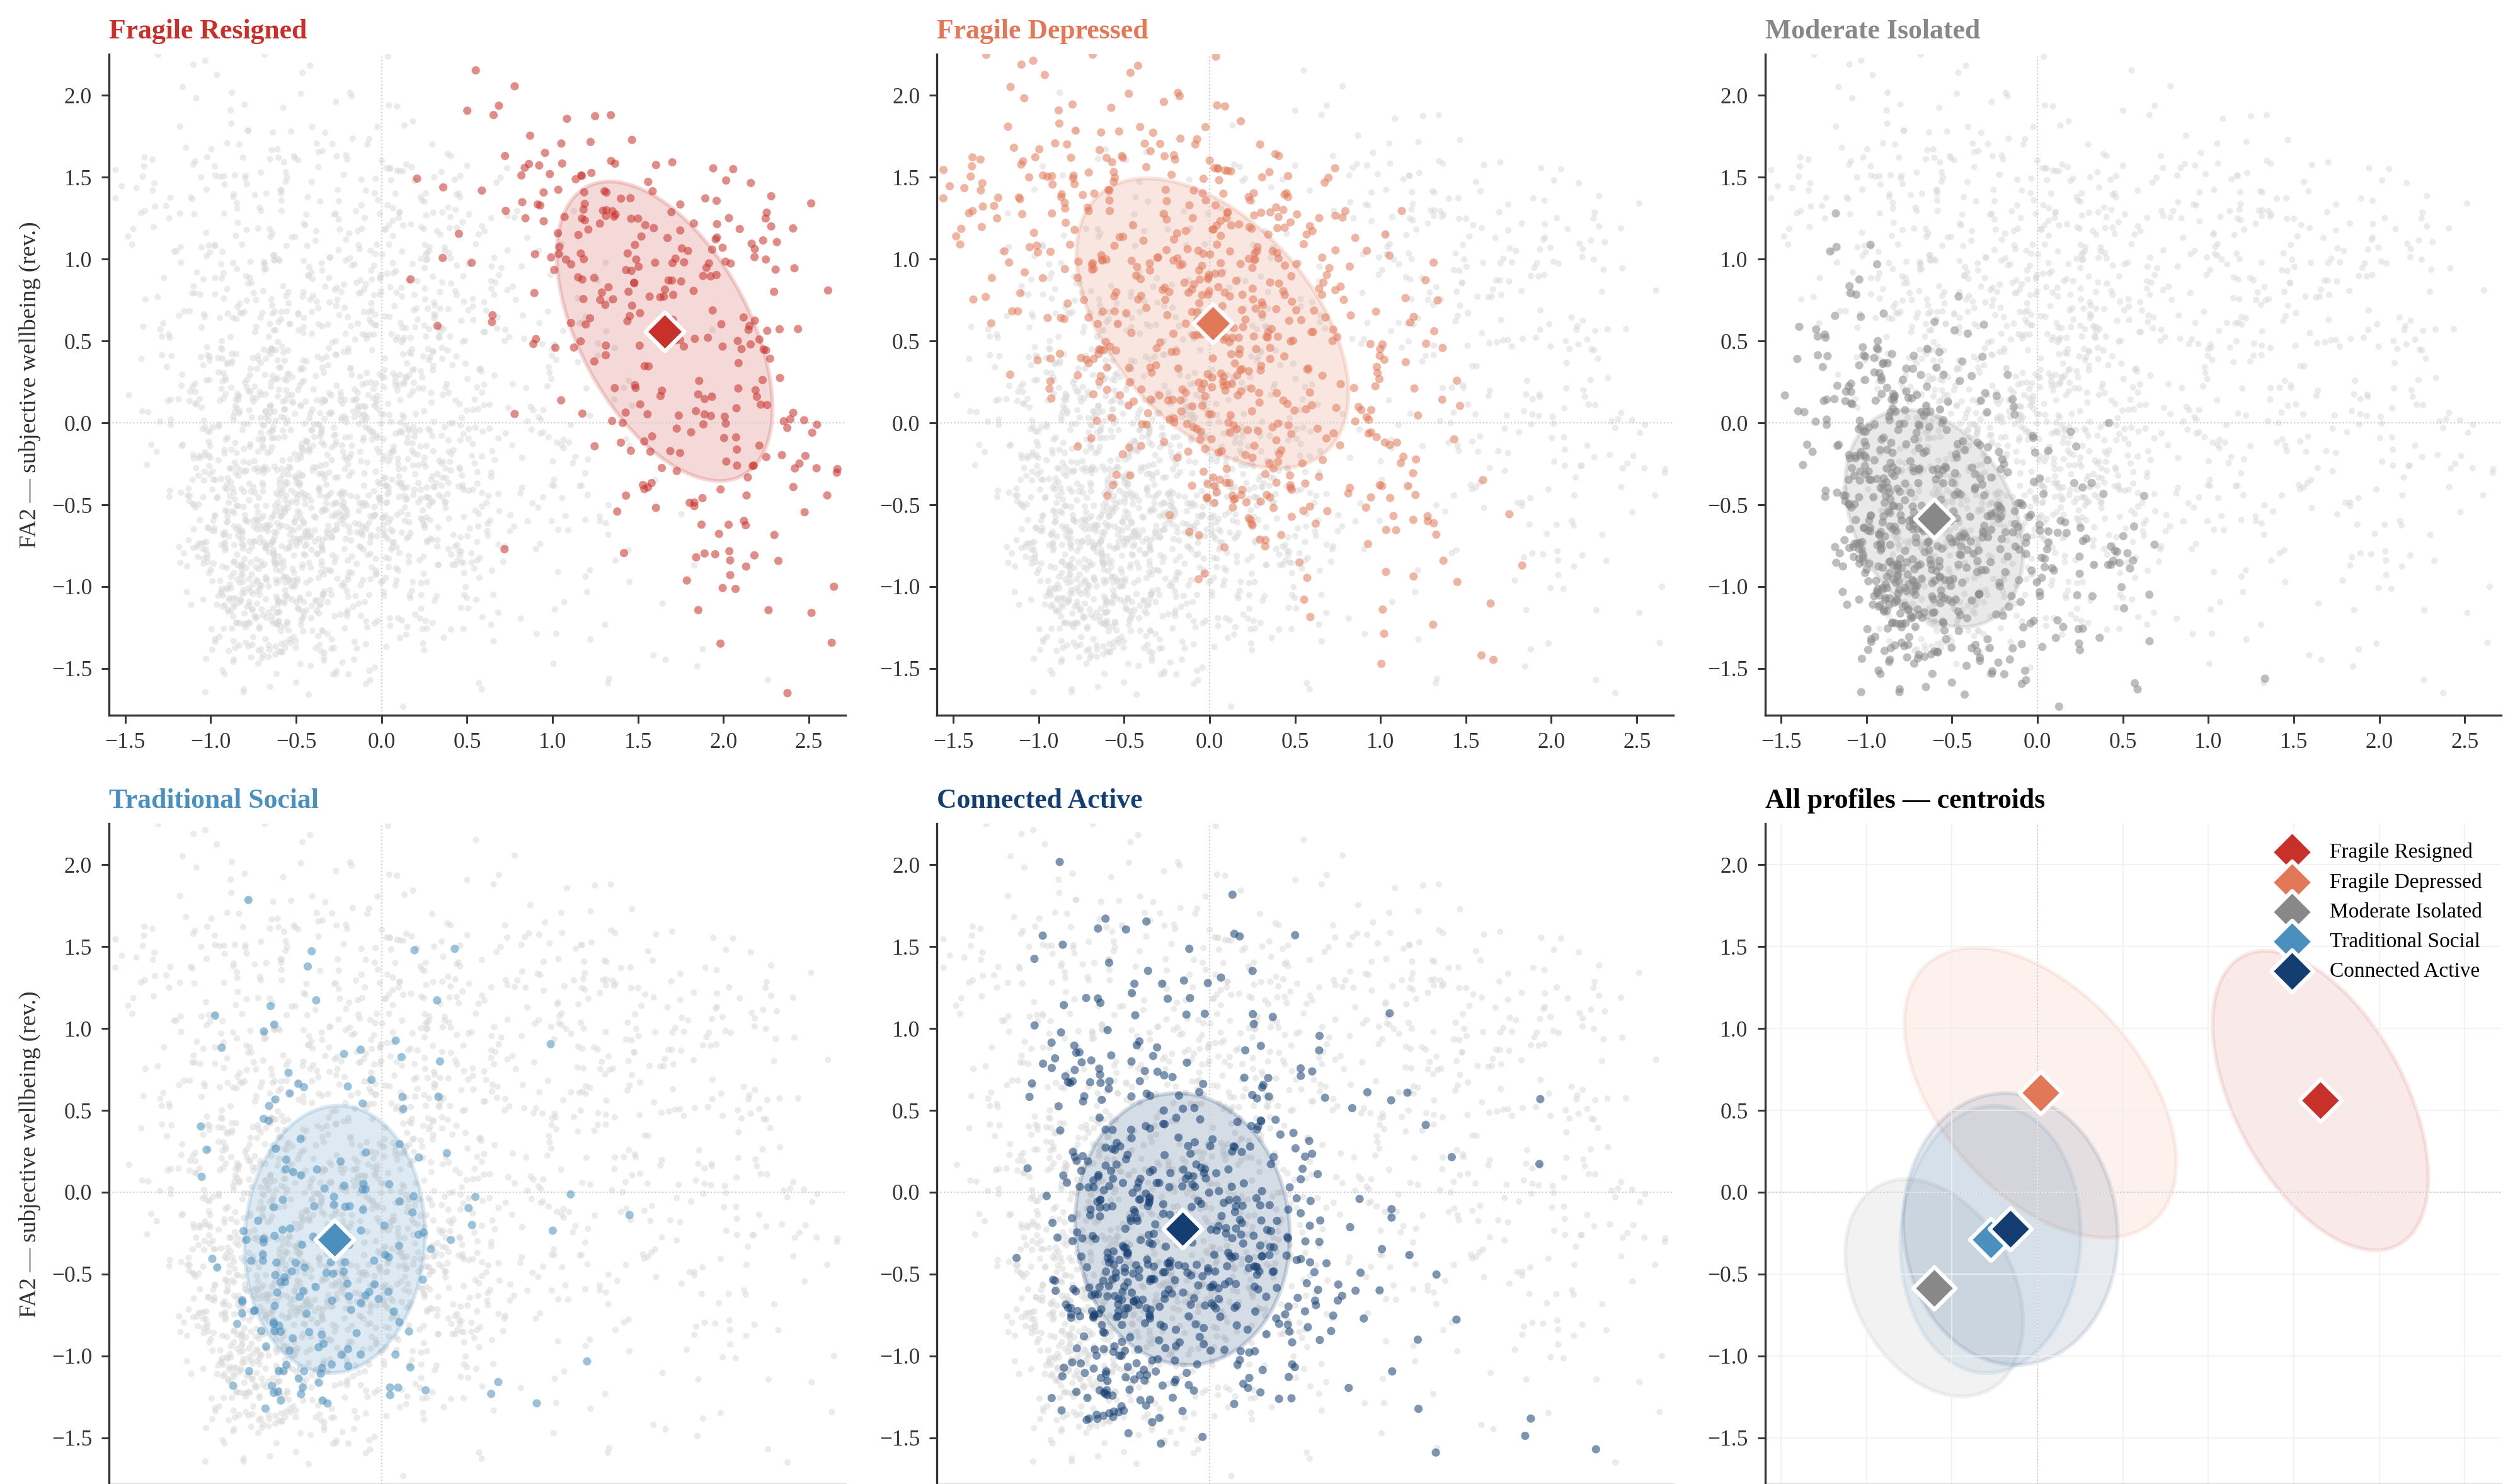
\includegraphics[width=0.95\linewidth]{figures/04_italy/fig_fa_scatter_pa1_pa2_italy.png}
  \caption{Profile scatter on the FA1 $\times$ FA2 plane, Italy. Each point is one Italian respondent positioned on the two dominant factors (FA1 = physical and functional fragility; FA2 = high values correspond to worse subjective wellbeing). Diamonds mark cluster centroids; ellipses mark 50\% confidence regions per profile.}
  \label{fig:ch4-fa-scatter}
\end{figure}

The visual reading of Figures~\ref{fig:ch4-fingerprint} and \ref{fig:ch4-fa-scatter} confirms the three-fold structure of the typology. The two fragile profiles lie above zero on health-burden variables and below zero on resource and digital variables, with Fragile Resigned systematically further from zero than Fragile Depressed. The Moderate Isolated and Traditional Social profiles overlap closely on resources and health and diverge sharply on social and digital engagement --- the country-specific Italian middle-stratum split. The Connected Active profile reaches the resource-and-digital pole on FA1 while remaining centred on FA2 --- the ``successful aging'' shape. The FA1 $\times$ FA2 scatter confirms that the five profiles occupy distinct regions of the latent space rather than a single severity gradient --- the visual counterpart of the substantive argument of \S\ref{sec:ch4-profile-descriptions}.

\section{External validation: life satisfaction}
\label{sec:ch4-external-validation}

Life satisfaction (SHARE Wave 9 item AC012, eleven-point scale) is administered in a separate questionnaire block and is not part of the analytical input set, providing an external validation outcome (Chapter~3). Figure~\ref{fig:ch4-lifesat} reports the distribution across the five Italian archetypes with the F-statistic of a one-way ANOVA in the figure caption.

\begin{figure}[ht]
  \centering
  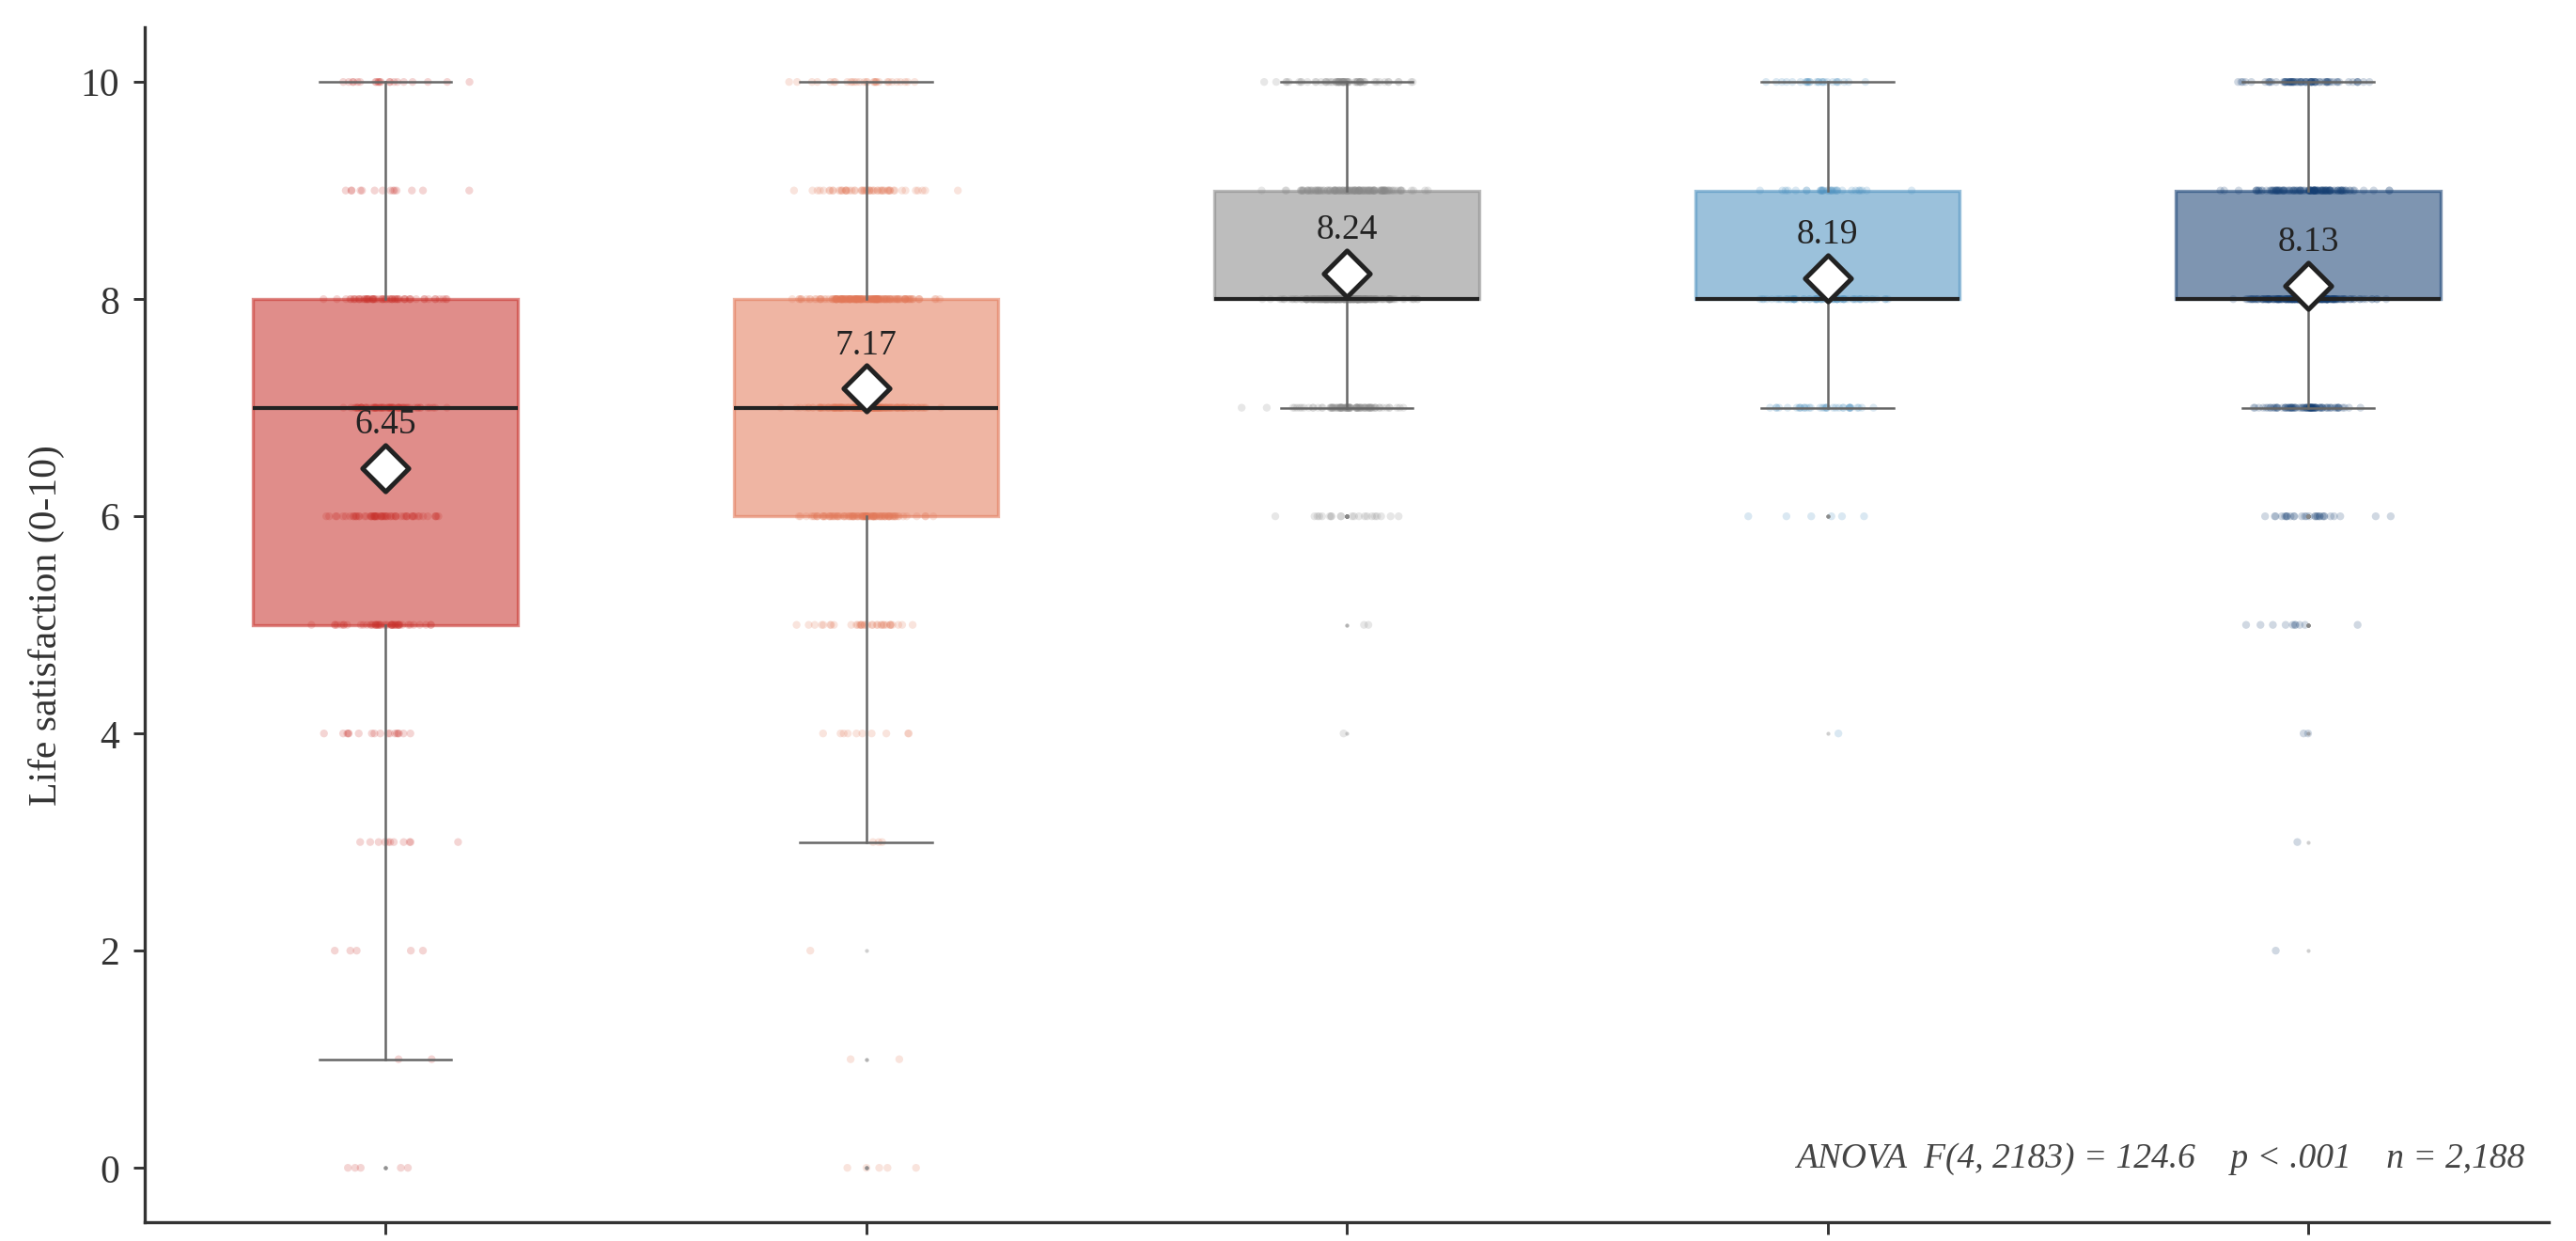
\includegraphics[width=0.95\linewidth]{figures/04_italy/fig_lifesat_anova_italy.png}
  \caption{Life satisfaction by profile, Italy. Boxplots of SHARE Wave 9 item AC012 (eleven-point scale, 0--10) by cluster membership; diamonds report cluster means. One-way ANOVA: $F(4, 2183) = 124.6$, $p < .001$. $n = 2{,}188$ (item-level non-response on lifesat reduces the analytical sample by 190 respondents from the 2,378 used for the segmentation).}
  \label{fig:ch4-lifesat}
\end{figure}

Mean life satisfaction is 6.5 in Fragile Resigned, 7.2 in Fragile Depressed, and clusters around 8.1--8.2 in the three non-fragile profiles, which are not statistically distinguishable from each other on this single item. The F-statistic of 124.6 on (4, 2183) degrees of freedom ($p < 0.001$) confirms substantial discriminative power of the typology on an outcome external to the input set. The lifesat outcome detects principally the binary contrast between fragile and non-fragile profiles (a roughly 1.5-point gap on the eleven-point scale); the within-non-fragile contrasts are minor --- consistent with the observation that life satisfaction in older age is dominated by the absence of major health and affective burdens. This supports the inclusion of the affective and evaluative subjective block as a constituent input to the typology, which preserves the within-fragile contrast (Fragile Resigned vs Fragile Depressed) that the lifesat outcome alone would not.

\section{Demographic distributions across profiles}
\label{sec:ch4-demographics}

The five archetypes are not uniformly distributed across gender and age. Figure~\ref{fig:ch4-gender} reports profile composition by gender on a 100\% stacked bar; Figure~\ref{fig:ch4-age} reports the parallel decomposition by age band (65--74, 75--84, 85+).

\begin{figure}[ht]
  \centering
  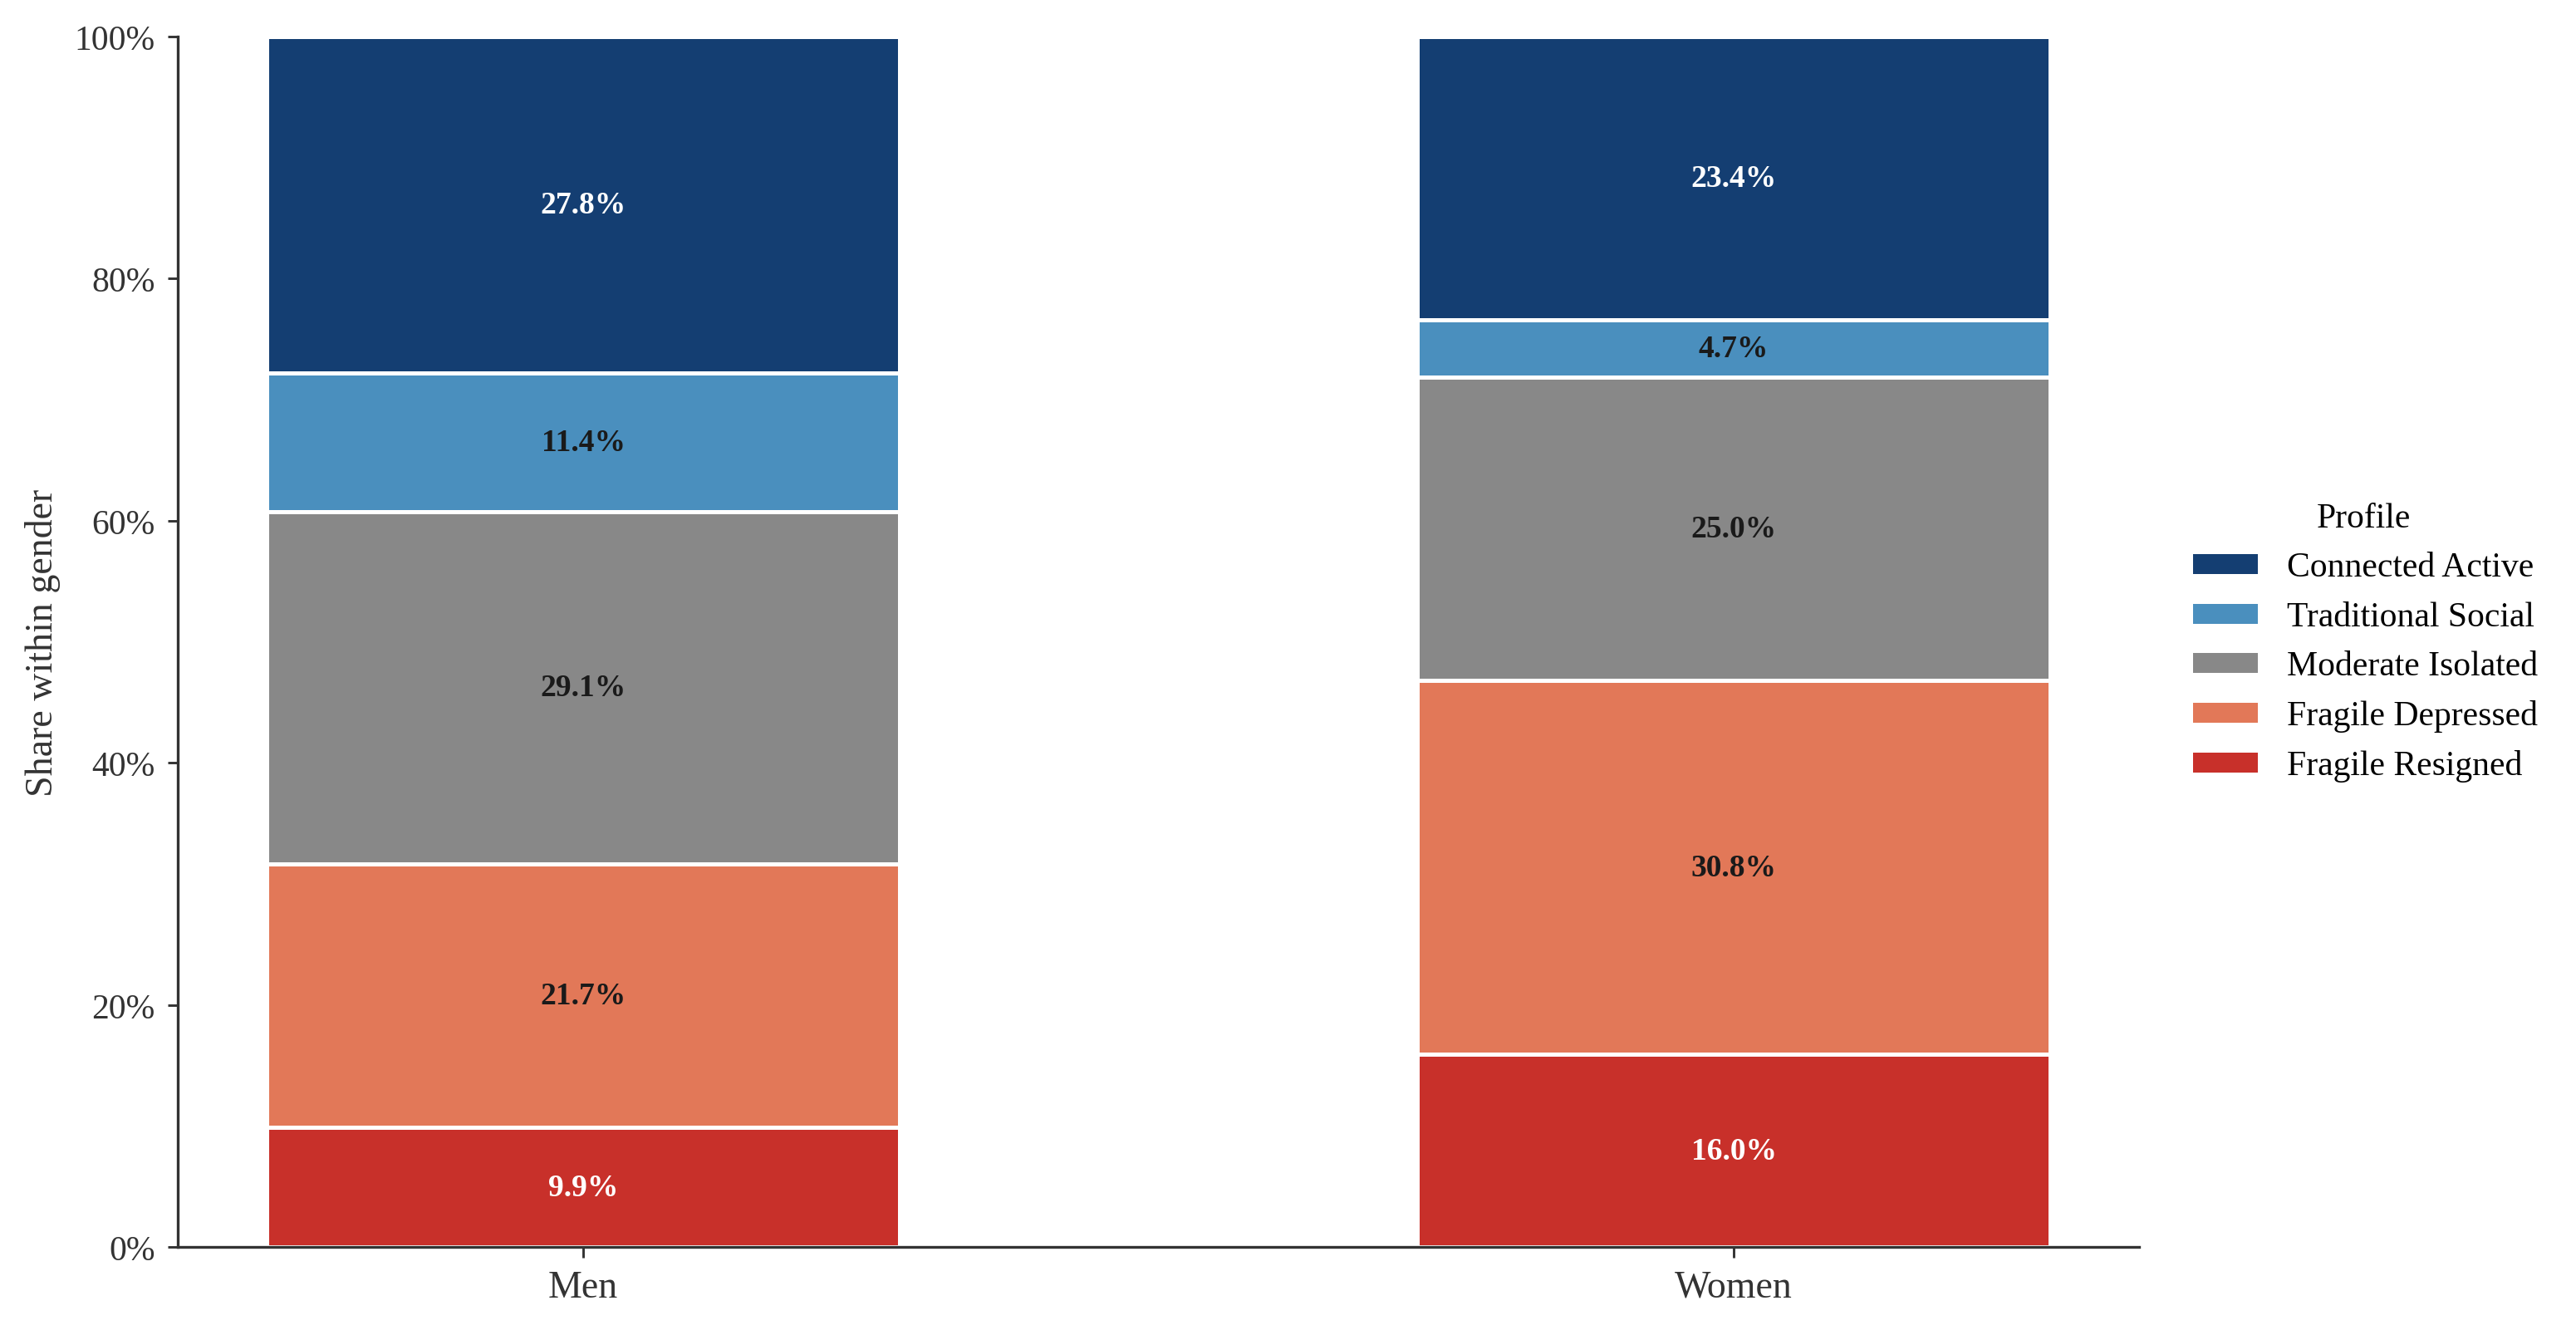
\includegraphics[width=0.95\linewidth]{figures/04_italy/fig_demographics_gender_italy.png}
  \caption{Profile composition by gender, Italy. Each column shows the percentage of the gender group falling in each archetype; columns sum to 100\%.}
  \label{fig:ch4-gender}
\end{figure}

\begin{figure}[ht]
  \centering
  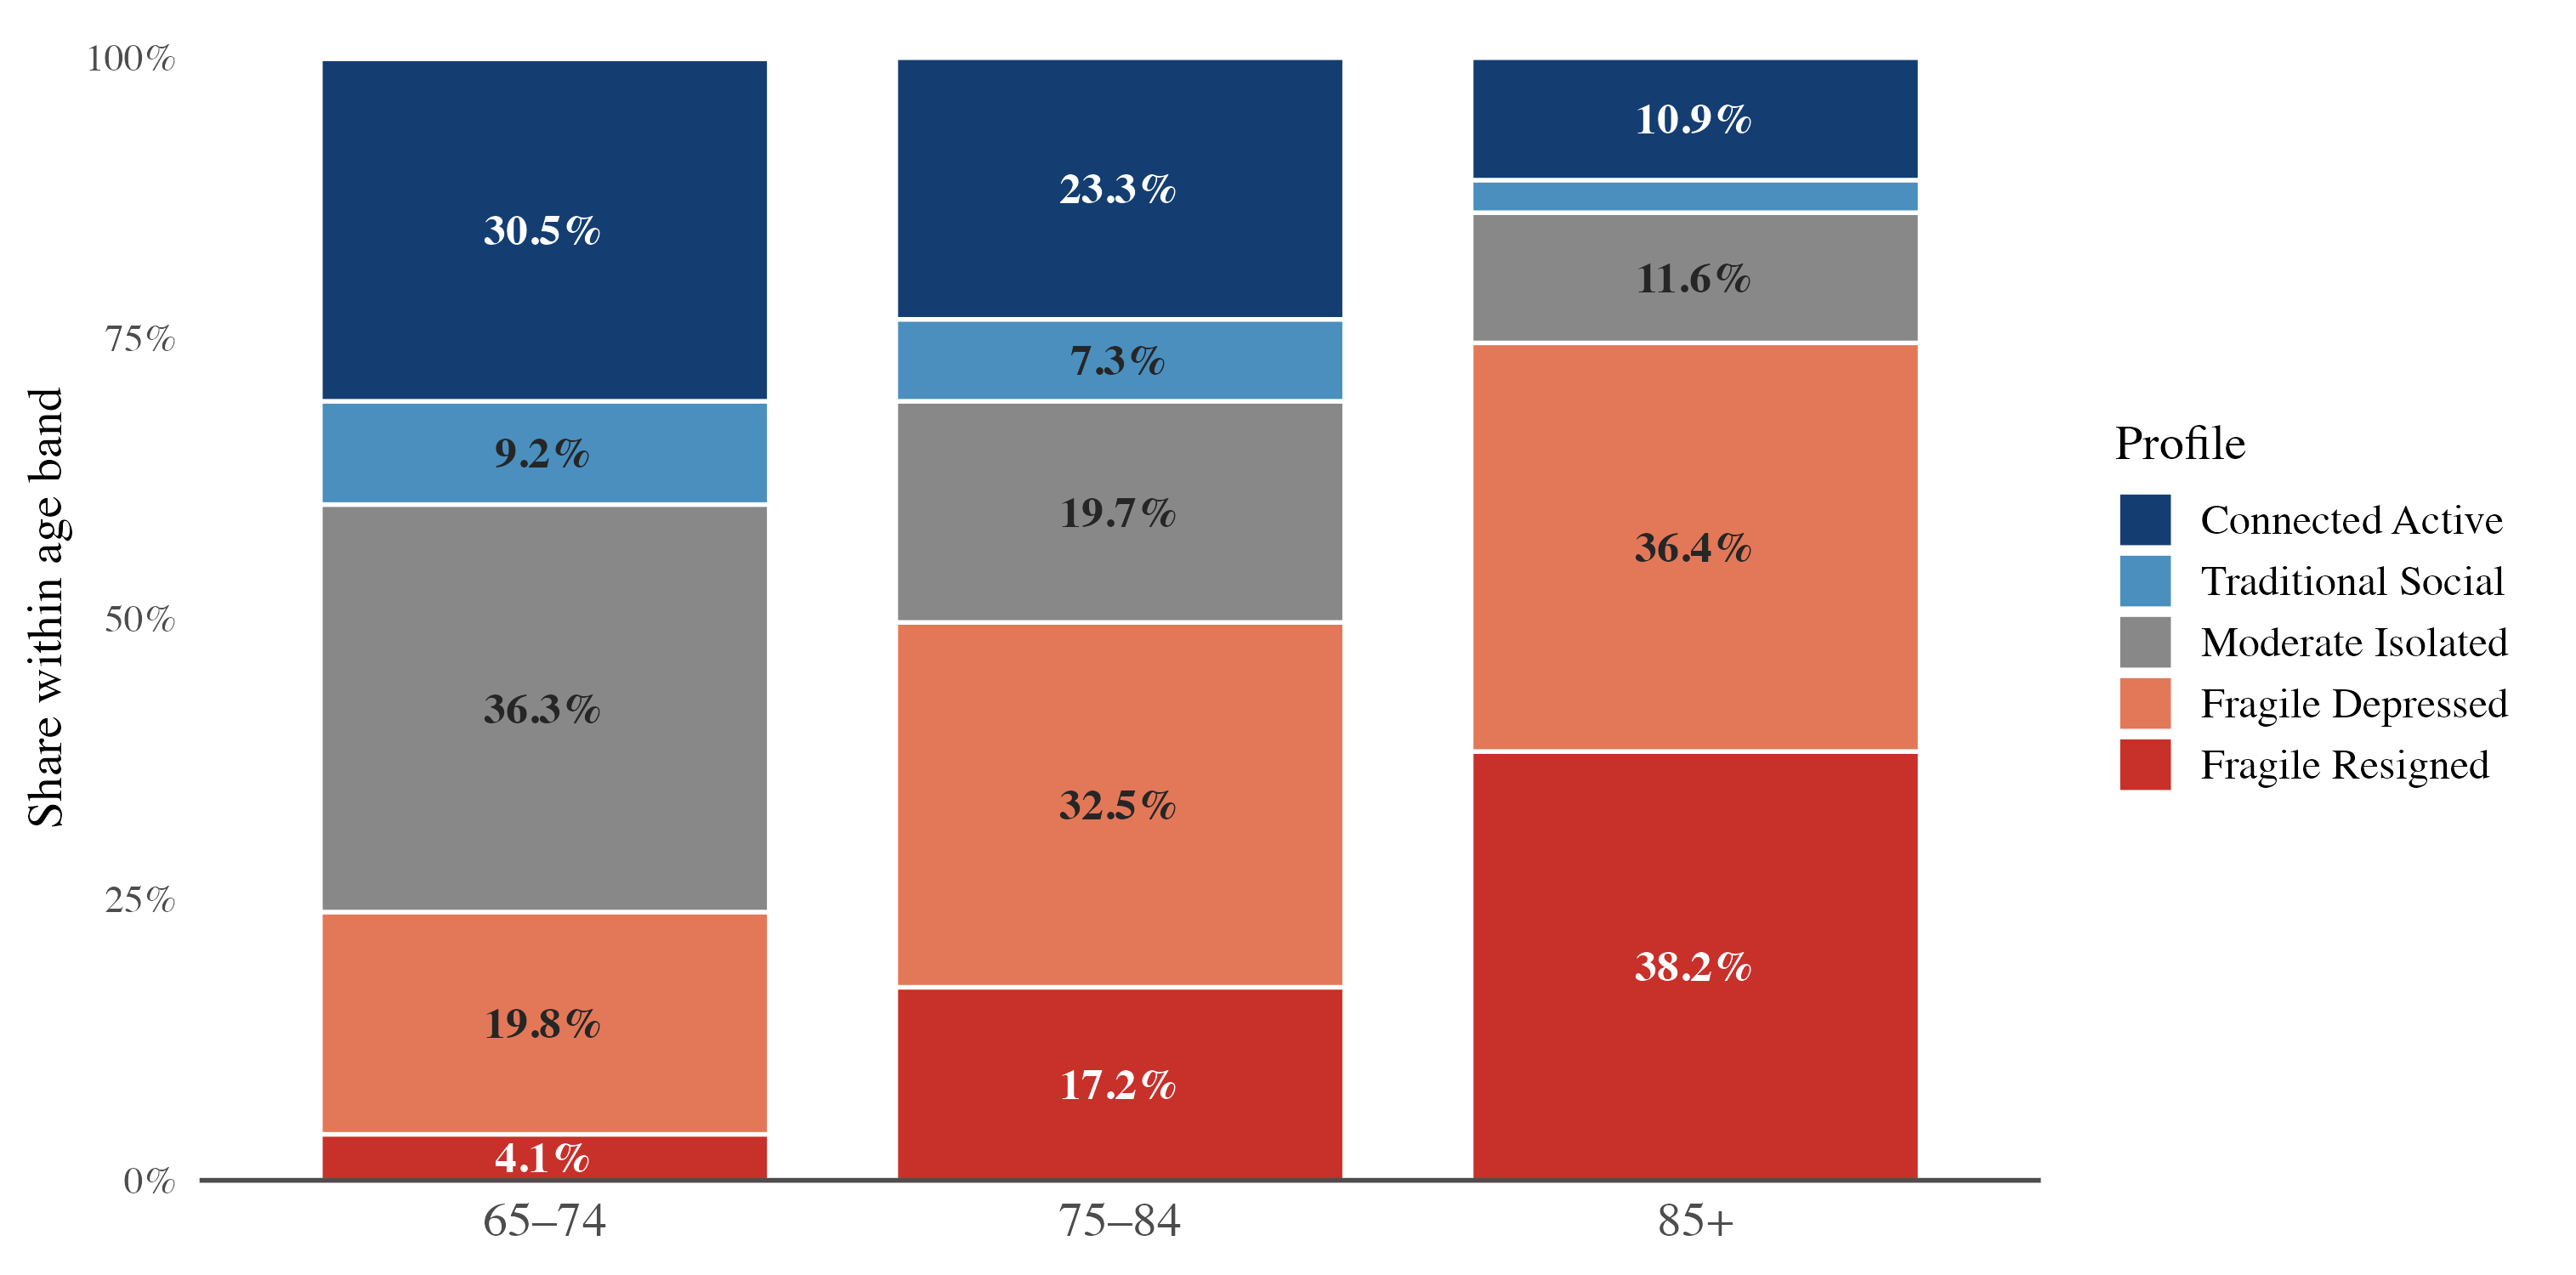
\includegraphics[width=0.95\linewidth]{figures/04_italy/fig_demographics_age_italy.png}
  \caption{Profile composition by age band, Italy. The Fragile Resigned share rises from 4\% in 65--74 to 38\% in 85+; the Connected Active share declines from 31\% to 11\% over the same range.}
  \label{fig:ch4-age}
\end{figure}

Two patterns emerge. First, the feminisation of fragility: 47\% of Italian over-65 women fall in one of the two fragile profiles (16\% Fragile Resigned + 31\% Fragile Depressed), against 32\% of men (10\% + 22\%). Conversely, 39\% of men are in the high-resource profiles (28\% Connected Active + 11\% Traditional Social), against 28\% of women. The pattern is consistent with the broader epidemiological literature on the differential aging of Italian women --- longer life expectancy paired with higher widowhood rates, lower lifetime labour-market attachment, lower individual pension income \citep{dykstra2009, pampel2001}.

Second, the age gradient is strong. In the 65--74 band, 31\% of respondents are in the Connected Active cluster and only 4\% in Fragile Resigned; in the 85+ band, the proportions are reversed (11\% Connected Active, 38\% Fragile Resigned). The Fragile Depressed share also increases monotonically with age (20\% $\to$ 33\% $\to$ 36\%); the Moderate Isolated share declines from 36\% to 12\%, reflecting the cohort transition from socially-disengaged but functionally autonomous late-young-old to functionally impaired oldest-old respondents. The most vulnerable sub-population (women, oldest old, fragile) is also the sub-population for whom standard digital channels of the silver economy are essentially inaccessible without family or institutional intermediation --- a finding with direct implications for the design of long-term-care services and digital products targeting the Italian over-65 population.

\section{The Isolation Paradox}
\label{sec:ch4-isolation-paradox}

The most distinctive finding of the Italian typology --- and one of the three original contributions of this thesis articulated in Chapter~1 --- is what we term the Isolation Paradox: the existence in Italy of a substantial population segment that is functionally and economically autonomous but socially and digitally disconnected, and that systematically under-utilises the healthcare system relative to peers with comparable health and resources but denser social engagement. The segment is the Moderate Isolated archetype described in \S\ref{sec:ch4-moderate-isolated}, with 28.1\% population share and approximately 3.98 million individuals.

\subsection{The empirical signature}
\label{sec:ch4-isolation-empirical}

The Moderate Isolated cluster shares with the Traditional Social cluster three core configurations: comparable health (mobility 0.6 vs 0.9 raw count, EURO-D 1.2 vs 1.7), comparable economic resources (log\_thinc within 0.7 z-score units), and comparable subjective evaluation of life (CASP 36.8 vs 38.5; both above the Italian mean). The two clusters diverge sharply on the social, cultural and digital engagement dimensions: the Moderate Isolated cluster is at $z = -0.22$ on network size against $+0.14$ for Traditional Social; at $z = -0.11$ on internet use against $+0.53$ for Traditional Social; at $z$ between $-0.15$ and $-0.37$ on cultural-engagement indicators against $+0.43$ to $+3.29$. In raw figures: 2.3 confidants vs 2.6, 34.1\% internet use vs 65.8\%, half the cultural-event participation rate. Despite these differences, the two clusters report the same mean life satisfaction (8.2 vs 8.2) --- the social isolation is not internalised as a deficit by the affected individuals on standard subjective-well-being indicators.

\subsection{The healthcare under-utilisation pattern}
\label{sec:ch4-isolation-healthcare}

The Isolation Paradox is substantiated by the analysis of healthcare utilisation across the two middle-stratum clusters, reported in detail in Chapter~6. Relative to Traditional Social, Moderate Isolated reports 1.36 fewer doctor visits per year, 0.72 fewer specialist visits, a 0.4 percentage-point higher rate of forgone care (respondents who report having needed but not received medical attention), and 2.02 fewer nights in hospital per year. The pattern is consistent across age bands and regions and survives adjustment for chronic-condition count, self-rated health, and economic resources. The combined effect is a systematic disengagement from the formal healthcare system, with the segment dropping below population averages on preventive, outpatient and inpatient indicators alike --- a configuration consistent with structural detachment from care channels rather than with delayed care-seeking.

\begin{figure}[ht]
  \centering
  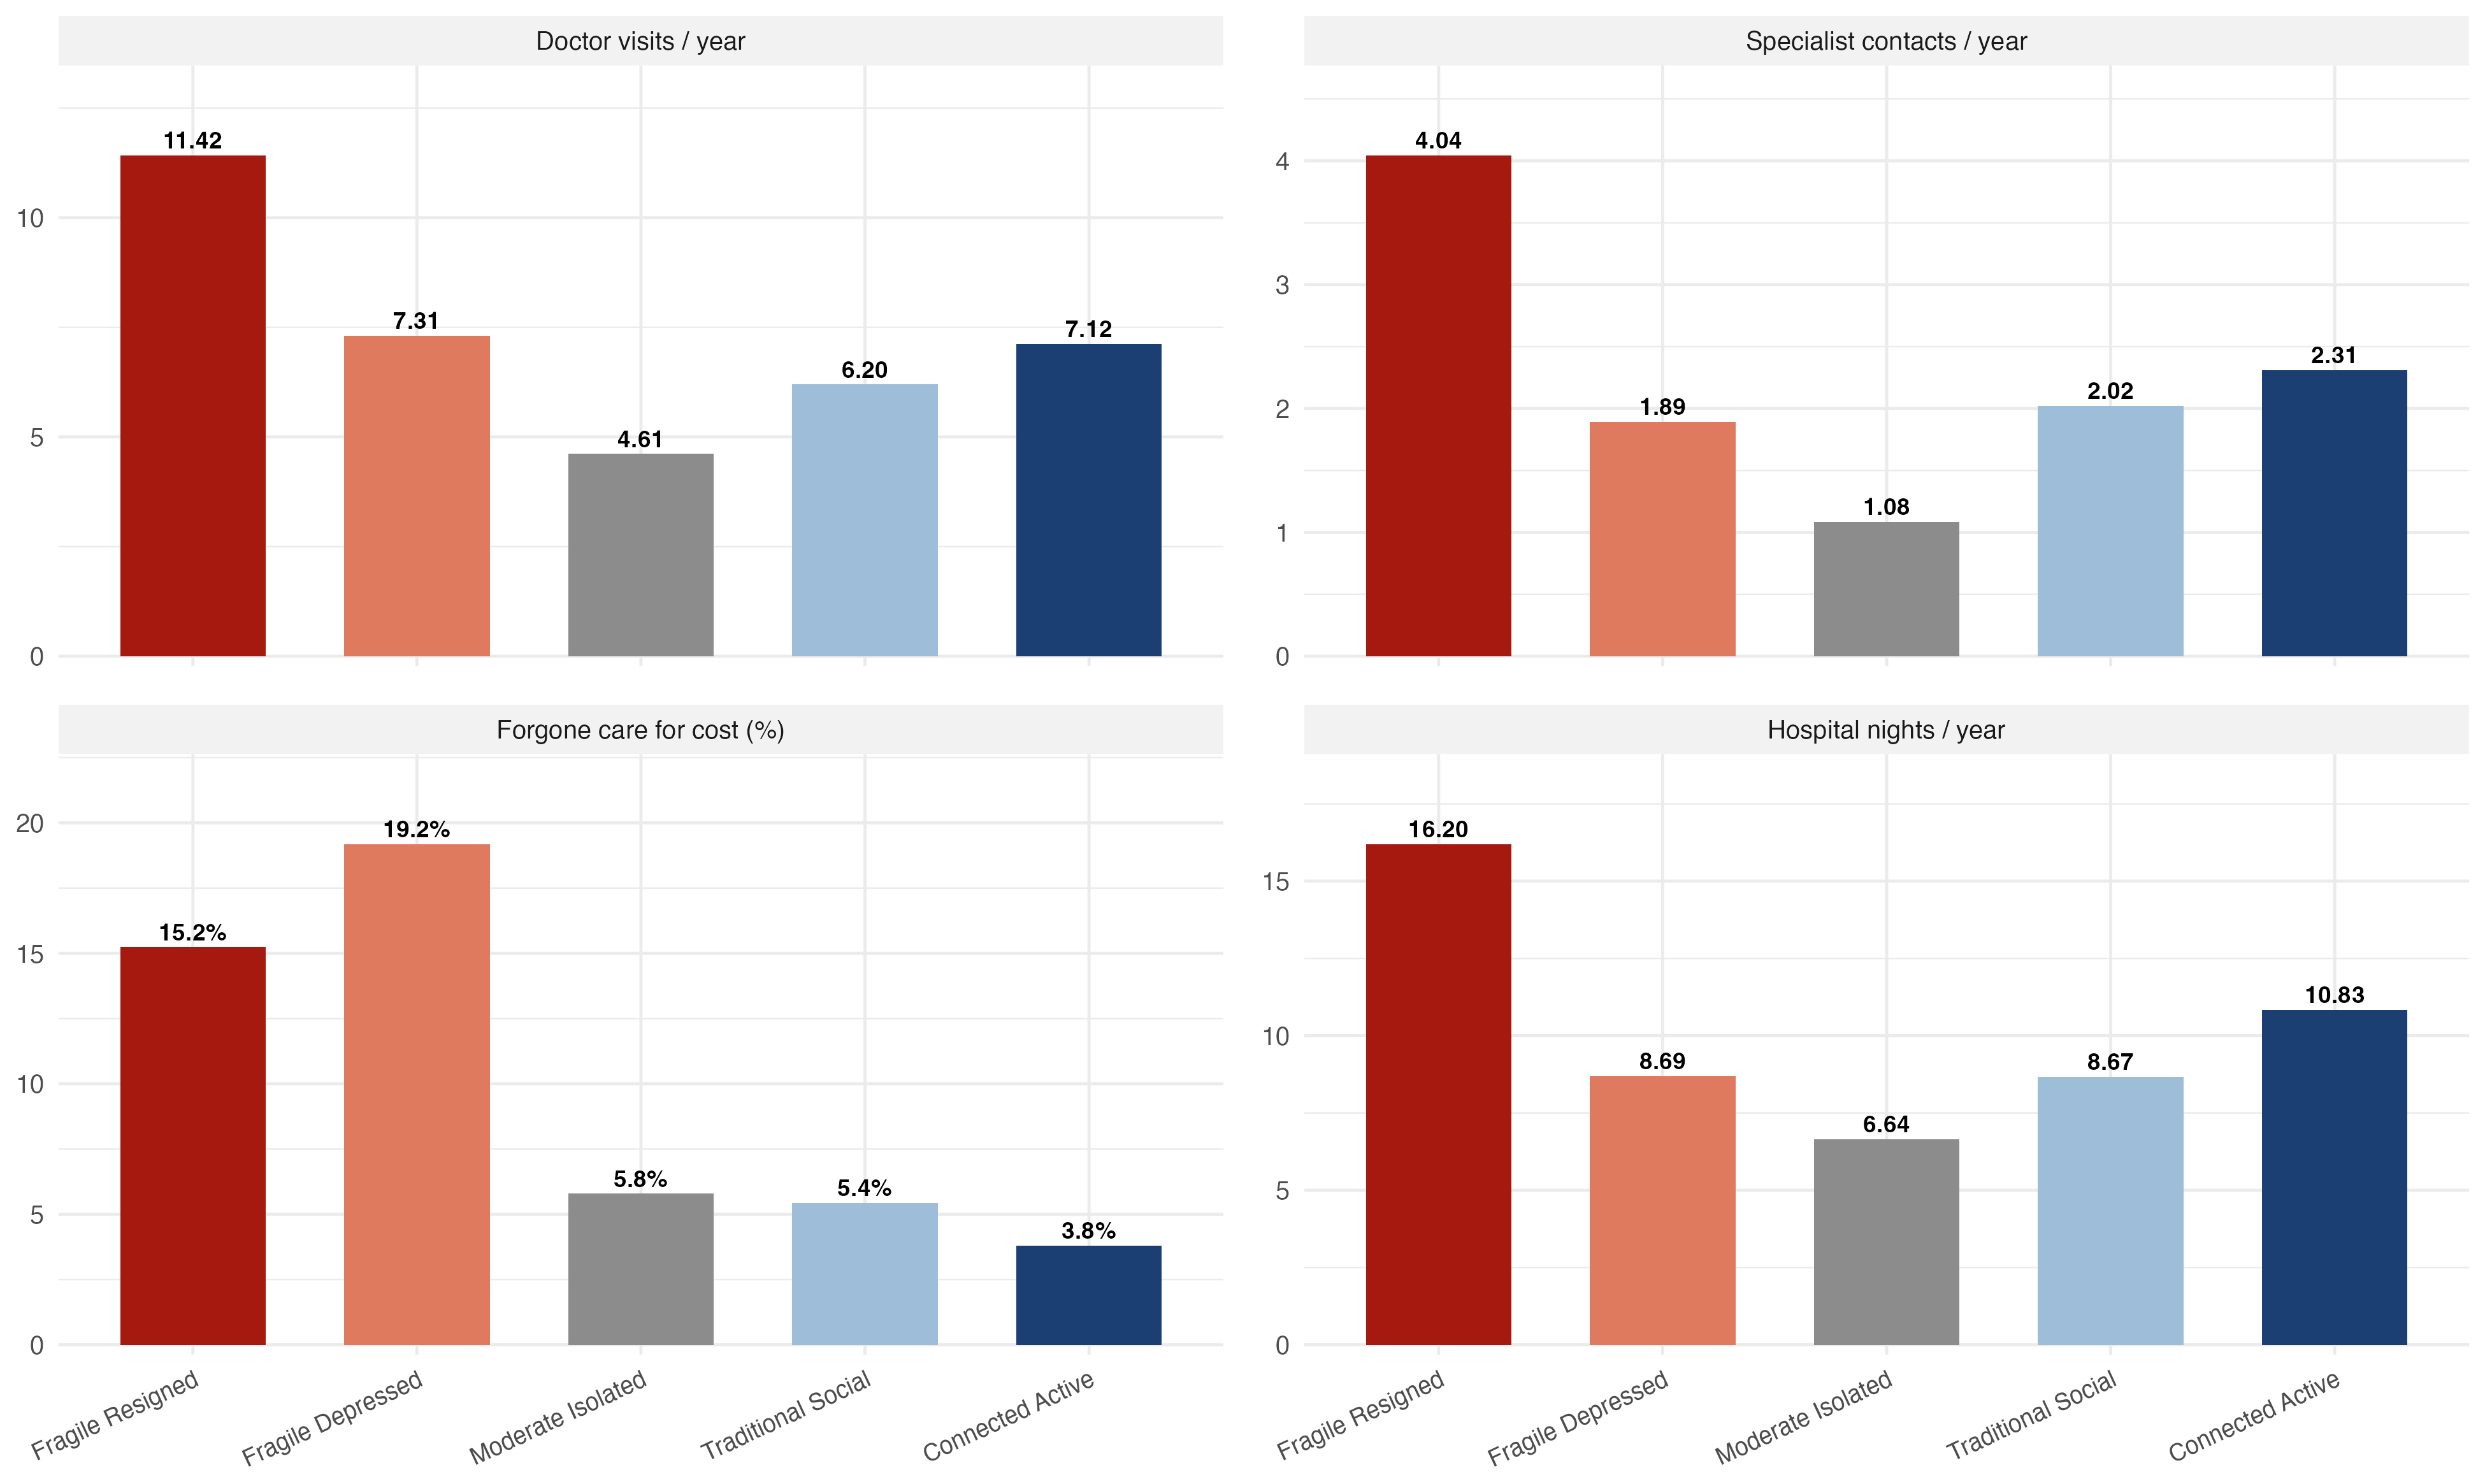
\includegraphics[width=0.95\linewidth]{figures/04_italy/fig_healthcare_italy.png}
  \caption{Healthcare utilisation across the five Italian archetypes. Cluster means on four healthcare indicators (doctor visits, specialist visits, forgone care percentage, hospital nights). Note the Moderate Isolated under-utilisation of preventive and outpatient care paired with over-utilisation of inpatient care --- the empirical signature of the Isolation Paradox (\S\ref{sec:ch4-isolation-paradox}).}
  \label{fig:ch4-healthcare}
\end{figure}

The mechanism is consistent with three convergent literatures. The literature on social capital and healthcare access \citep{berkmankawachi2000, putnam2000} documents the role of dense social networks in transmitting symptom information and signposting individuals towards appropriate care. The gerontological literature on the gateway role of grandchildren and adult children in mediating digital and informational access of older adults \citep{quanhaase2017} identifies a role that the Moderate Isolated cluster, with its thin family-network structure, is by definition unable to leverage. The Italian welfare-state literature on regional fragmentation of public health services \citep{loscalzo2009} makes informal social capital a more critical input for healthcare navigation than in welfare regimes designed for universal access.

\subsection{Why the Paradox is Italian-only}
\label{sec:ch4-isolation-italian-only}

The Isolation Paradox does not have a structural counterpart in the Swedish typology of Chapter~5. The Swedish Moderate archetype is socially integrated at a level comparable to the Swedish population mean, with internet use above 90\% and network size at the population mean. The Hungarian-matched cross-country analysis of Chapter~6 confirms that the Moderate Isolated cluster has no Swedish twin within a structural distance $\leq 2.0$ in standardised space --- it is a country-specific Italian phenomenon. The reading is that the Moderate Isolated configuration emerges where the welfare regime substitutes individual responsibility and family-based provision for universal-access institutions \citep{espingandersen1990, ferrera1996}. In Italy, individuals not embedded in a dense family or community network face a thin informational environment and a fragmented public-service infrastructure; in Sweden, the universal-access infrastructure provides a substitute baseline that prevents the emergence of an analogous configuration.

\subsection{Policy and silver-economy implications}
\label{sec:ch4-isolation-implications}

The Isolation Paradox has three implications for the design of services and technologies targeted at the Italian over-65 population. First, the size of the affected segment (3.98 million individuals) makes it a first-order policy and market reality, not a residual category. Second, the segment is not characterised by health or economic adversity that would route it into the existing long-term-care or income-support branches of the Italian welfare system; it is invisible to those branches. Third, the segment is not characterised by the absence of digital channels in absolute terms (34.1\% internet use is non-trivial); it is characterised by the absence of social and informational mediation that would route the available digital channels towards healthcare and service utilisation. The implication for silver-economy product design is that the Moderate Isolated segment is not addressable by direct-to-consumer digital products in the same way as the Connected Active segment; product designs that combine a digital channel with a social-mediation layer (peer-network platforms, community-based digital intermediaries, family-network-augmented service interfaces) are the candidate operational solution. The strategic case for this product-design gap as an opportunity for innovation in the Italian silver economy is developed in Chapter~6.

\section{Synthesis}
\label{sec:ch4-synthesis}

The Italian typology partitions the over-65 population into five archetypes spanning an interpretable severity gradient on health and resources, an orthogonal affective contrast within the fragile stratum, and an orthogonal cultural-versus-digital contrast within the high-resource stratum. The five archetypes are unequally distributed (28.1\% in the largest cluster, 11.7\% in the smallest), with population-projected sizes from 1.66 million (Fragile Depressed) to 3.98 million (Moderate Isolated). External validation against life satisfaction confirms substantial discriminative power ($F(4, 2183) = 124.6$, $p < 0.001$).

Three findings of substantive importance emerge. The qualitative distinction between Fragile Resigned and Fragile Depressed identifies two distinct configurations with different functional and affective signatures, calling for distinct policy responses (long-term-care provision in the first case, mental-health services in the second). The country-specific Moderate Isolated archetype --- the largest single cluster at 28.1\% --- identifies a substantial fraction of the Italian over-65 population whose late-life experience is socially and digitally thin. The Isolation Paradox documents that this segment, despite being functionally and economically autonomous, systematically under-utilises preventive and outpatient healthcare and over-utilises inpatient care, in a pattern consistent with the welfare-regime literature on Italian familism and the gerontological literature on social capital and healthcare access. The next chapter develops the parallel typology for Sweden; Chapter~6 maps the four matched cross-country pairs and develops the comparative reading of the Isolation Paradox; Chapter~7 reports the full battery of robustness diagnostics.

\begin{figure}[ht]
  \centering
  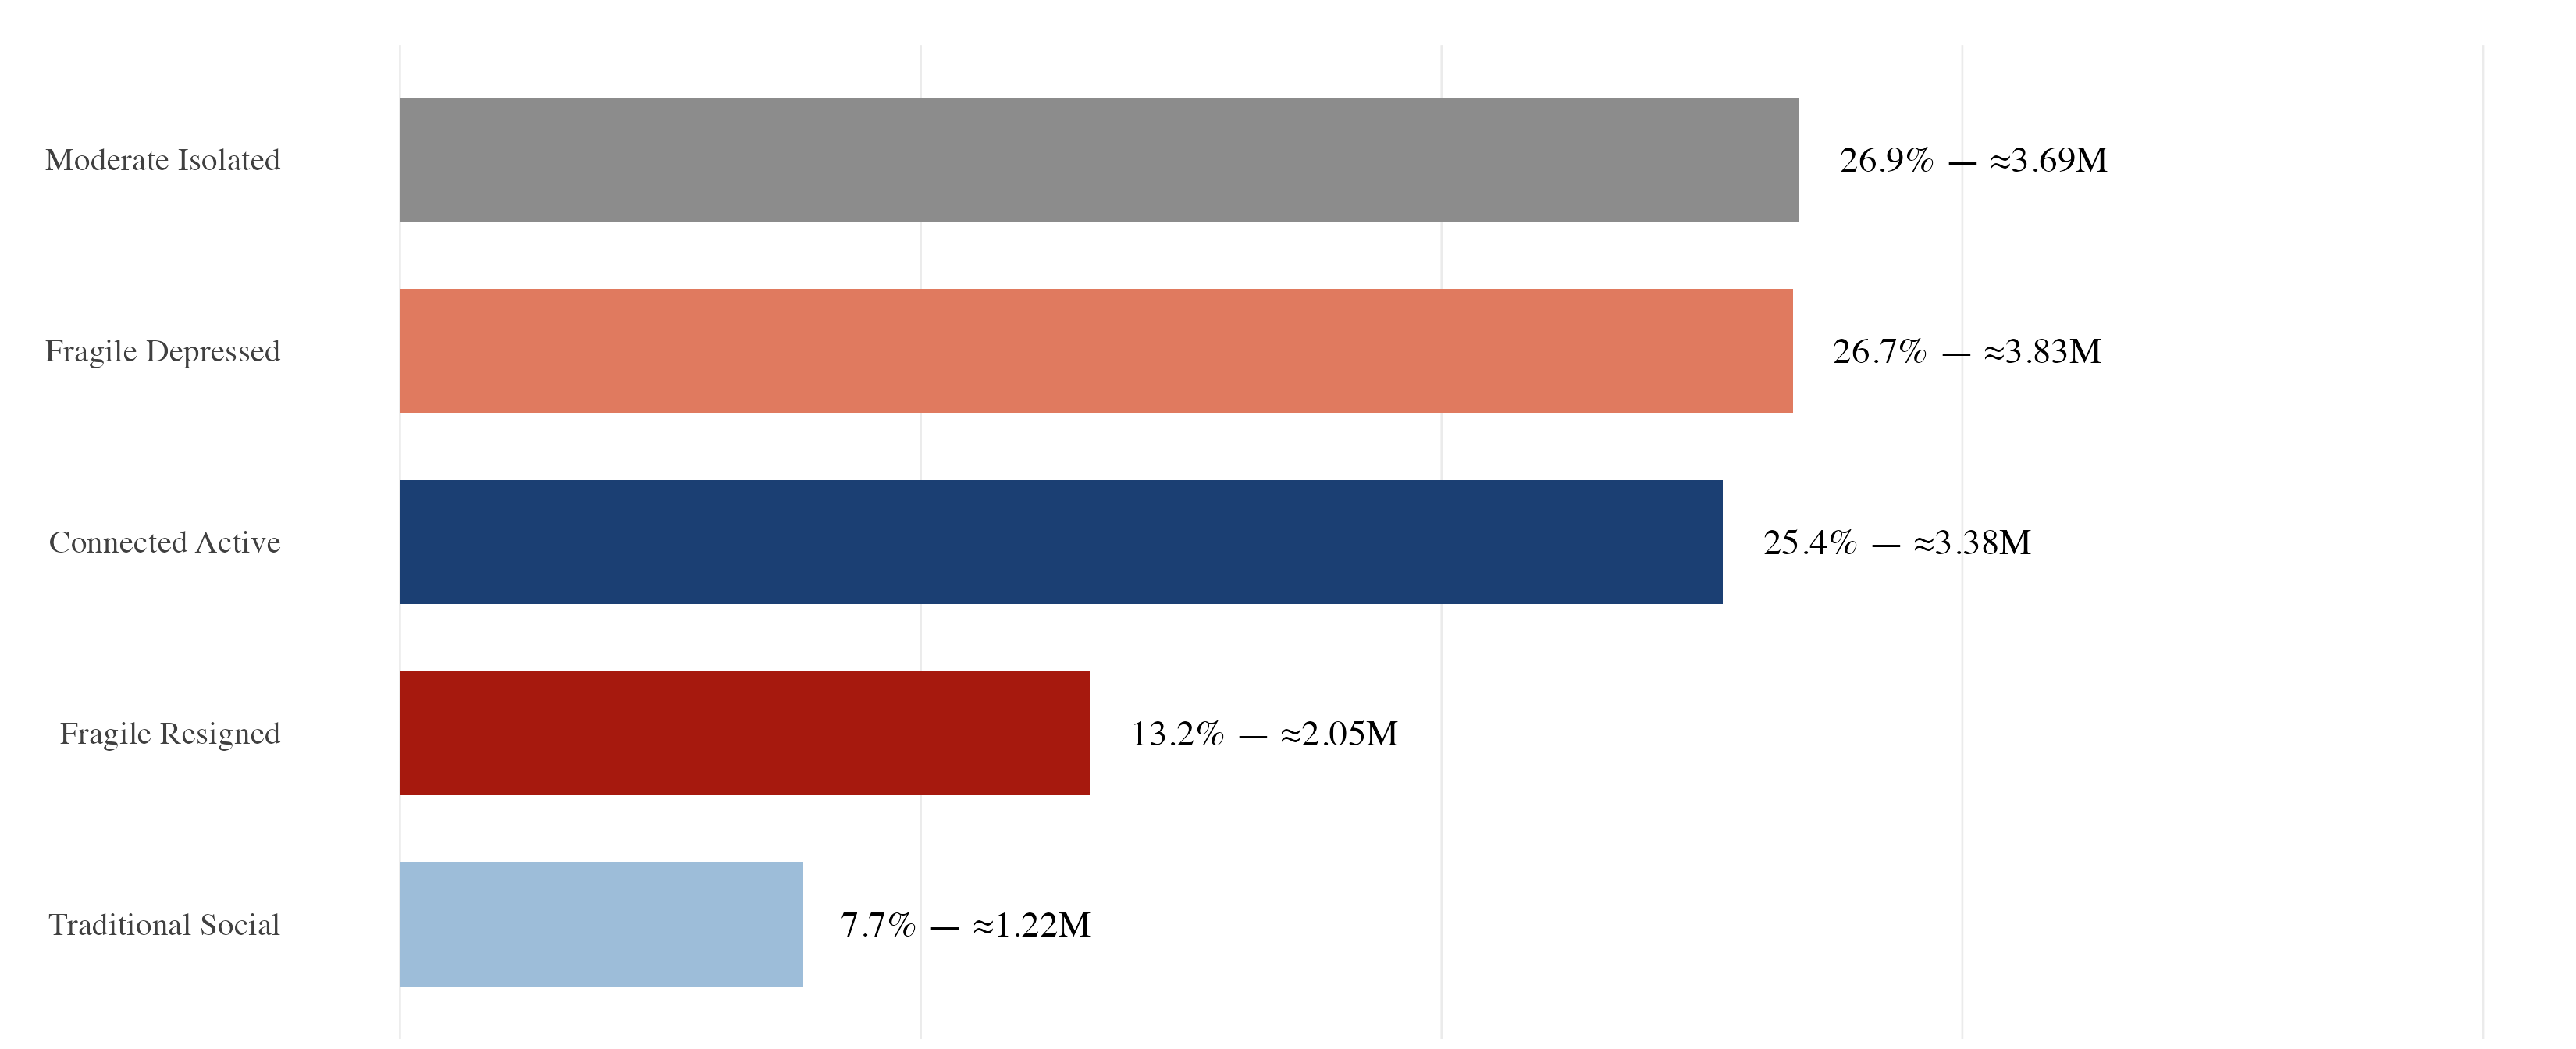
\includegraphics[width=0.95\linewidth]{figures/04_italy/fig_4_8_NEW.png}
  \caption{Population shares of the five Italian archetypes. Bar chart of within-sample shares projected to the Istat 2024 estimate of 14.18 million Italian residents aged 65 or older.}
  \label{fig:ch4-shares}
\end{figure}


\chapter{Cross-country comparison: Italy and Sweden}
\label{ch:ch5}

This chapter extends the segmentation framework of Chapter~\ref{ch:ch4} to Sweden, applying identical preprocessing and clustering rules on the Swedish sub-sample, and then compares the two country segmentations at the profile level. The comparison is motivated by the polar welfare-regime contrast --- Italy's familistic model against Sweden's universalist model (Esping-Andersen, 1990; Ferrera, 1996) --- and the expectation that the same analytical pipeline should yield profile structures that rhyme across countries while differing systematically in levels.

\section{The six Swedish profiles}
\label{sec:ch5-swedish-profiles}

The Swedish analytical sample comprises $n = 1{,}787$ respondents, obtained from the $2{,}202$ first-implicate over-65 Swedes after complete-case listwise deletion ($n = 2{,}045$) and the removal of 258 Mahalanobis outliers at the $\chi^{2}$ cut-off of $p = 0.001$ with 31 degrees of freedom. Unlike Italy, Sweden retains all thirty-one analytical variables in the clustering input: \emph{ac035d4} and \emph{ac035d7} exhibit low but non-zero variance (four to six per cent positive responses) and therefore contribute to the analysis.

K-means with $k = 6$ on the standardised-variable matrix yields six interpretable profiles (Table~\ref{tab:ch5-swedish-profiles}). The solution is retained at $k = 6$ without the micro-cluster removal step applied to Italy, since no micro-cluster smaller than five per cent of the sample emerges from the Swedish fit.

\begin{table}[ht]
  \centering
  \caption{Swedish profile sizes and cluster means on key variables ($n = 1{,}787$).}
  \label{tab:ch5-swedish-profiles}
  \small
  \begin{tabular}{@{}lrrrrrrrr@{}}
    \toprule
    \textbf{Profile} & \textbf{n} & \textbf{\%} & \textbf{Age} & \textbf{Internet} & \textbf{CASP} & \textbf{Lone.} & \textbf{Hope} & \textbf{LifeSat}\\
    \midrule
    Fragile            & 206 & 11.5 & 80.4 & 0.64 & 33.6 & 4.9 & 0.81 & 7.42\\
    Social Decline     & 149 &  8.3 & 72.6 & 0.99 & 40.3 & 3.5 & 0.98 & 8.51\\
    Moderate           & 417 & 23.3 & 76.6 & 0.94 & 37.1 & 3.8 & 0.91 & 8.06\\
    Asset Rich         & 341 & 19.1 & 77.7 & 0.75 & 39.3 & 3.8 & 0.96 & 8.48\\
    Wealthy Digital    & 138 &  7.7 & 74.9 & 0.96 & 40.3 & 3.5 & 0.99 & 8.47\\
    Connected Wealthy  & 536 & 30.0 & 73.1 & 0.99 & 42.1 & 3.3 & 0.99 & 8.88\\
    \bottomrule
  \end{tabular}
  \par\smallskip
  \footnotesize \emph{Note.} Internet and Hope are binary proportions. Profile ordering within the table is alphabetical; the substantive ordering in the text follows CASP ascending from Fragile to Connected Wealthy.
\end{table}

Two features distinguish the Swedish segmentation from the Italian one. First, three out of six Swedish profiles have internet penetration above 94\% --- a level that in Italy is approached only by Connected Active. Second, even the most fragile Swedish profile (Fragile, CASP = 33.6) reports subjective well-being comparable to the Italian Fragile Depressed (CASP = 30.7) or Moderate Isolated (CASP = 36.8) profiles, confirming a structural welfare-regime gap that is visible across the entire distribution rather than concentrated at the margins.

\subsection{Fragile}
The smallest and oldest profile ($n = 206$; 11.5\%; mean age 80.4) is the Swedish counterpart of the Italian Fragile Resigned: low CASP (33.6), high loneliness (4.9), reduced hope (81\%). Internet use is 64\%, dramatically higher than the Italian Fragile Resigned (9\%) at comparable age and clinical conditions.
\subsection{Social Decline}
A compact profile ($n = 149$; 8.3\%) characterised by intact digital integration (99\% internet) but elevated loneliness (3.5) and a CASP of 40.3. It is the Swedish analogue of the Italian Fragile Depressed.
\subsection{Moderate}
The largest middle-aged profile ($n = 417$; 23.3\%) combines good health, average digital use (94\%), and moderate social integration (loneliness 3.8, CASP 37.1). It maps onto the Italian Traditional Social in the matched-pair framework introduced below.
\subsection{Asset Rich}
A wealth-driven profile ($n = 341$; 19.1\%) with high life satisfaction (8.48) but below-average internet use (75\%) and smaller social networks than Connected Wealthy. It has no Italian analogue and is one of the two welfare-regime-specific Swedish types.
\subsection{Wealthy Digital}
The smallest Swedish profile ($n = 138$; 7.7\%) combines very high internet use (96\%), high CASP (40.3), and strong hope (99\%). Like Asset Rich, this is a Swedish-specific type with no Italian counterpart.
\subsection{Connected Wealthy}
The largest Swedish profile ($n = 536$; 30.0\%) represents the upper tail of the distribution: near-universal internet use (99\%), lowest loneliness (3.3), highest CASP (42.1), highest life satisfaction (8.88). It is the Swedish counterpart of the Italian Connected Active.

\section{Matched-pair comparison}
\label{sec:ch5-matched-pairs}

The cross-country comparison uses the four matched pairs introduced in Table~\ref{tab:ch3-matched-pairs}. Table~\ref{tab:ch5-gap} reports the Sweden-minus-Italy gap on seven outcome variables for each of the four pairs.

\begin{table}[ht]
  \centering
  \caption{Cross-country gap (Sweden minus Italy) on matched profile pairs.}
  \label{tab:ch5-gap}
  \small
  \begin{tabular}{@{}lrrrr@{}}
    \toprule
    \textbf{Variable} & \textbf{Fragile} & \textbf{Declining} & \textbf{Socially-oriented} & \textbf{Connected}\\
    \midrule
    CASP-12             & $+5.73$   & $+9.63$   & $-1.37$   & $+4.31$\\
    Loneliness (3--9)   & $-1.24$   & $-1.90$   & $+0.07$   & $-0.45$\\
    Internet (pp)       & $+55.0$   & $+81.4$   & $+28.0$   & $+23.7$\\
    Fluency             & $+8.67$   & $+13.61$  & $+4.18$   & $+7.30$\\
    Hope (pp)           & $+35.2$   & $+30.4$   & $+1.21$   & $+8.55$\\
    EURO-D (0--12)      & $-2.29$   & $-2.23$   & $+1.21$   & $-0.80$\\
    Life satisfaction   & $+0.97$   & $+1.34$   & $-0.13$   & $+0.76$\\
    \bottomrule
  \end{tabular}
  \par\smallskip
  \footnotesize \emph{Note.} Matched pairs: \emph{Fragile} = Fragile Resigned vs Fragile; \emph{Declining} = Fragile Depressed vs Social Decline; \emph{Socially-oriented} = Traditional Social vs Moderate; \emph{Connected} = Connected Active vs Connected Wealthy. Internet and Hope are expressed in percentage points (of the binary rate). Loneliness and EURO-D negative values mean Sweden is lower (less lonely, less depressed) than Italy.
\end{table}

Welch's $t$-tests on every cell of Table~\ref{tab:ch5-gap} confirm that all gaps in the Fragile, Declining and Connected pairs are statistically significant at $p < 0.01$, with most of them at $p < 10^{-15}$. The Socially-oriented pair is the only exception: on loneliness, Hope, and life satisfaction, Traditional Social Italians and Moderate Swedes are indistinguishable; on CASP, the Italian Traditional Social exceeds the Swedish Moderate by $1.37$ points ($p = 0.001$), the only case in which Italy \emph{leads} Sweden in the matched-pair design. Figure~\ref{fig:ch5-matched-pairs-gap} visualises the same comparison.

\begin{figure}[ht]
  \centering
  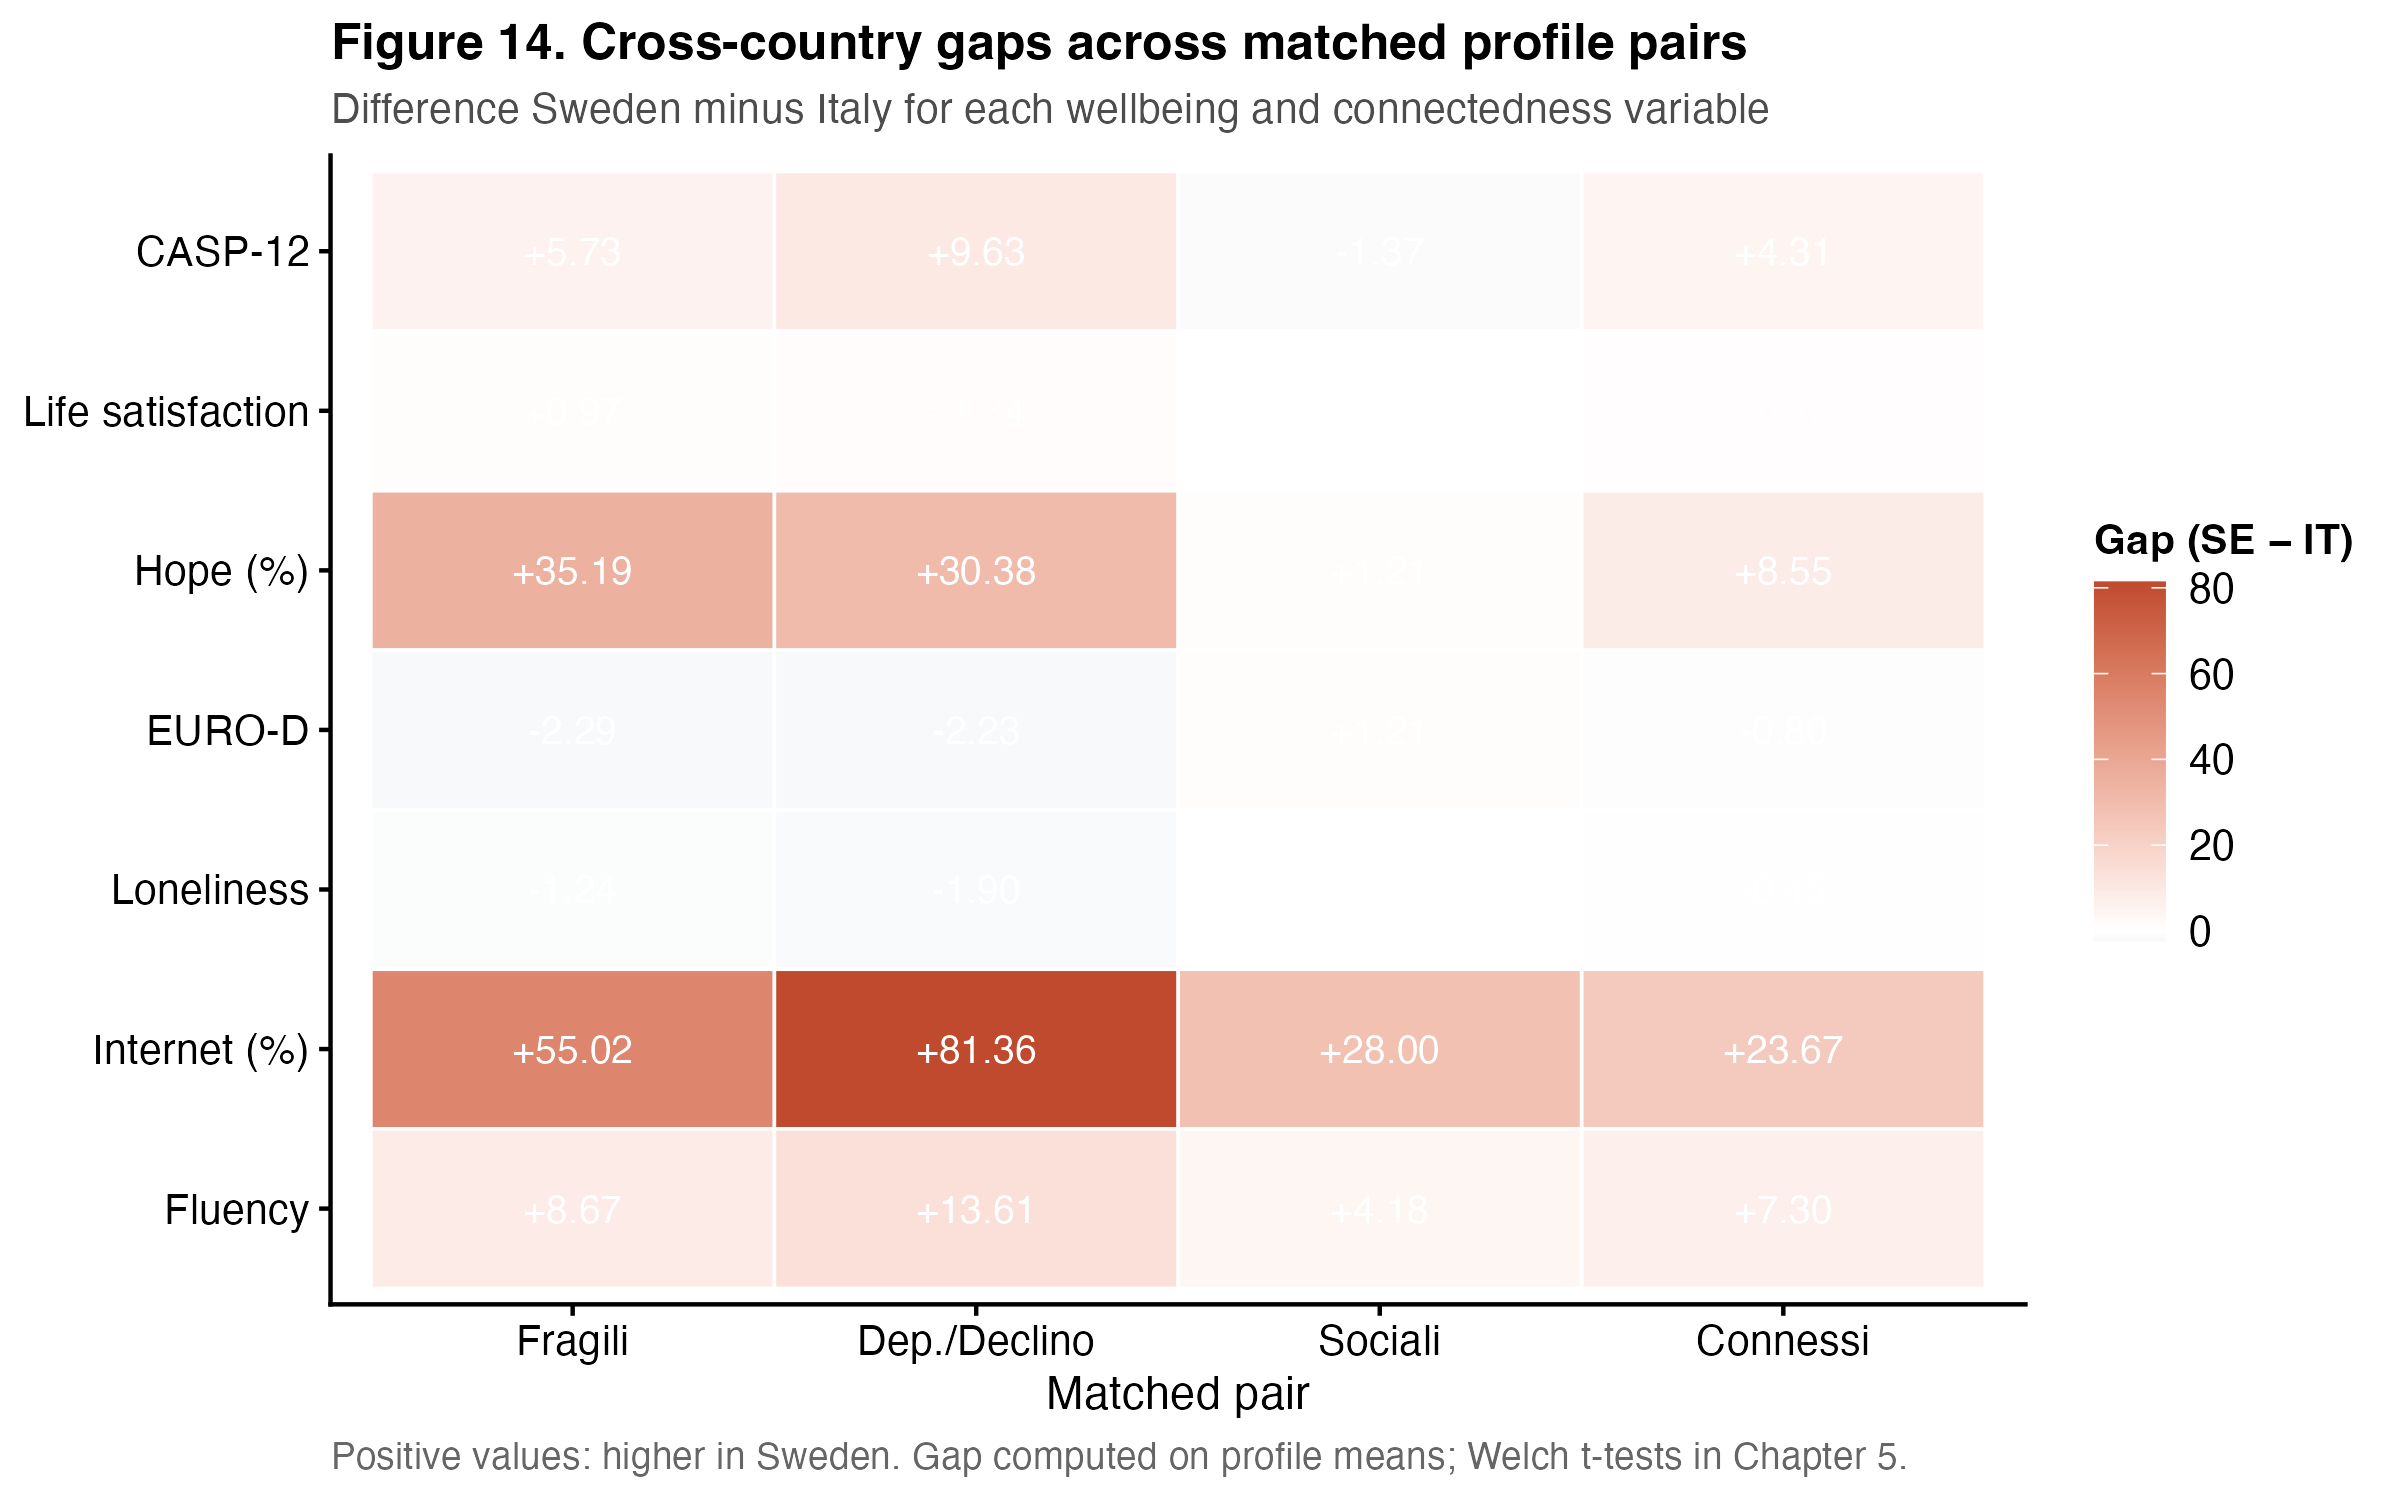
\includegraphics[width=0.90\linewidth]{figures/06_comparison/fig_14_matched_pairs_gap.png}
  \caption{Sweden-minus-Italy gap by matched pair, seven outcome variables. Source: v9 pipeline.}
  \label{fig:ch5-matched-pairs-gap}
\end{figure}

\section{The systematic Swedish-over-Italian gap}
\label{sec:ch5-gap}

The quantitative pattern of Table~\ref{tab:ch5-gap} can be summarised as follows. On CASP-12, Swedes exceed matched Italians by between $+4.31$ (Connected pair) and $+9.63$ (Declining pair), with the largest gap falling on the most vulnerable groups. On the internet variable, the gap ranges from $+23.7$ percentage points (Connected pair) to $+81.4$ points (Declining pair) --- essentially a wholesale transformation of the digital-access profile at the bottom of the distribution. On fluency, Swedes outperform Italians by 4 to 14 words per minute, with the same distribution-concentration pattern. On depression (EURO-D), Swedes score between $0.80$ and $2.29$ points lower, with the gap again largest among the most fragile.

The gap is therefore \emph{structural} rather than compositional: the same analytical pipeline applied to both samples reveals a Sweden-over-Italy shift that is preserved across profiles, rules out sample-level composition effects, and is largest at the vulnerable end of each distribution. The interpretation in terms of welfare-regime architecture is developed in Chapter~\ref{ch:ch8}.

\section{Welfare-regime-specific profiles}
\label{sec:ch5-unmatched}

Three profiles fall outside the matched-pair design and are interpreted as welfare-regime-specific types. The Italian \emph{Moderate Isolated} ($n = 639$) is the large objectively-healthy-but-socially-isolated group that is absent from the Swedish segmentation; its substantive importance is developed in Chapter~\ref{ch:ch7}. On the Swedish side, \emph{Asset Rich} ($n = 341$) and \emph{Wealthy Digital} ($n = 138$) are two prosperous profiles that occupy different positions in the digital-access space (75\% vs 96\% internet use, respectively) and in the social-network dimension; together they account for 26.8\% of the Swedish sample and have no Italian analogue. Figure~\ref{fig:ch5-country-unique} displays the unique profiles in each country.

\begin{figure}[ht]
  \centering
  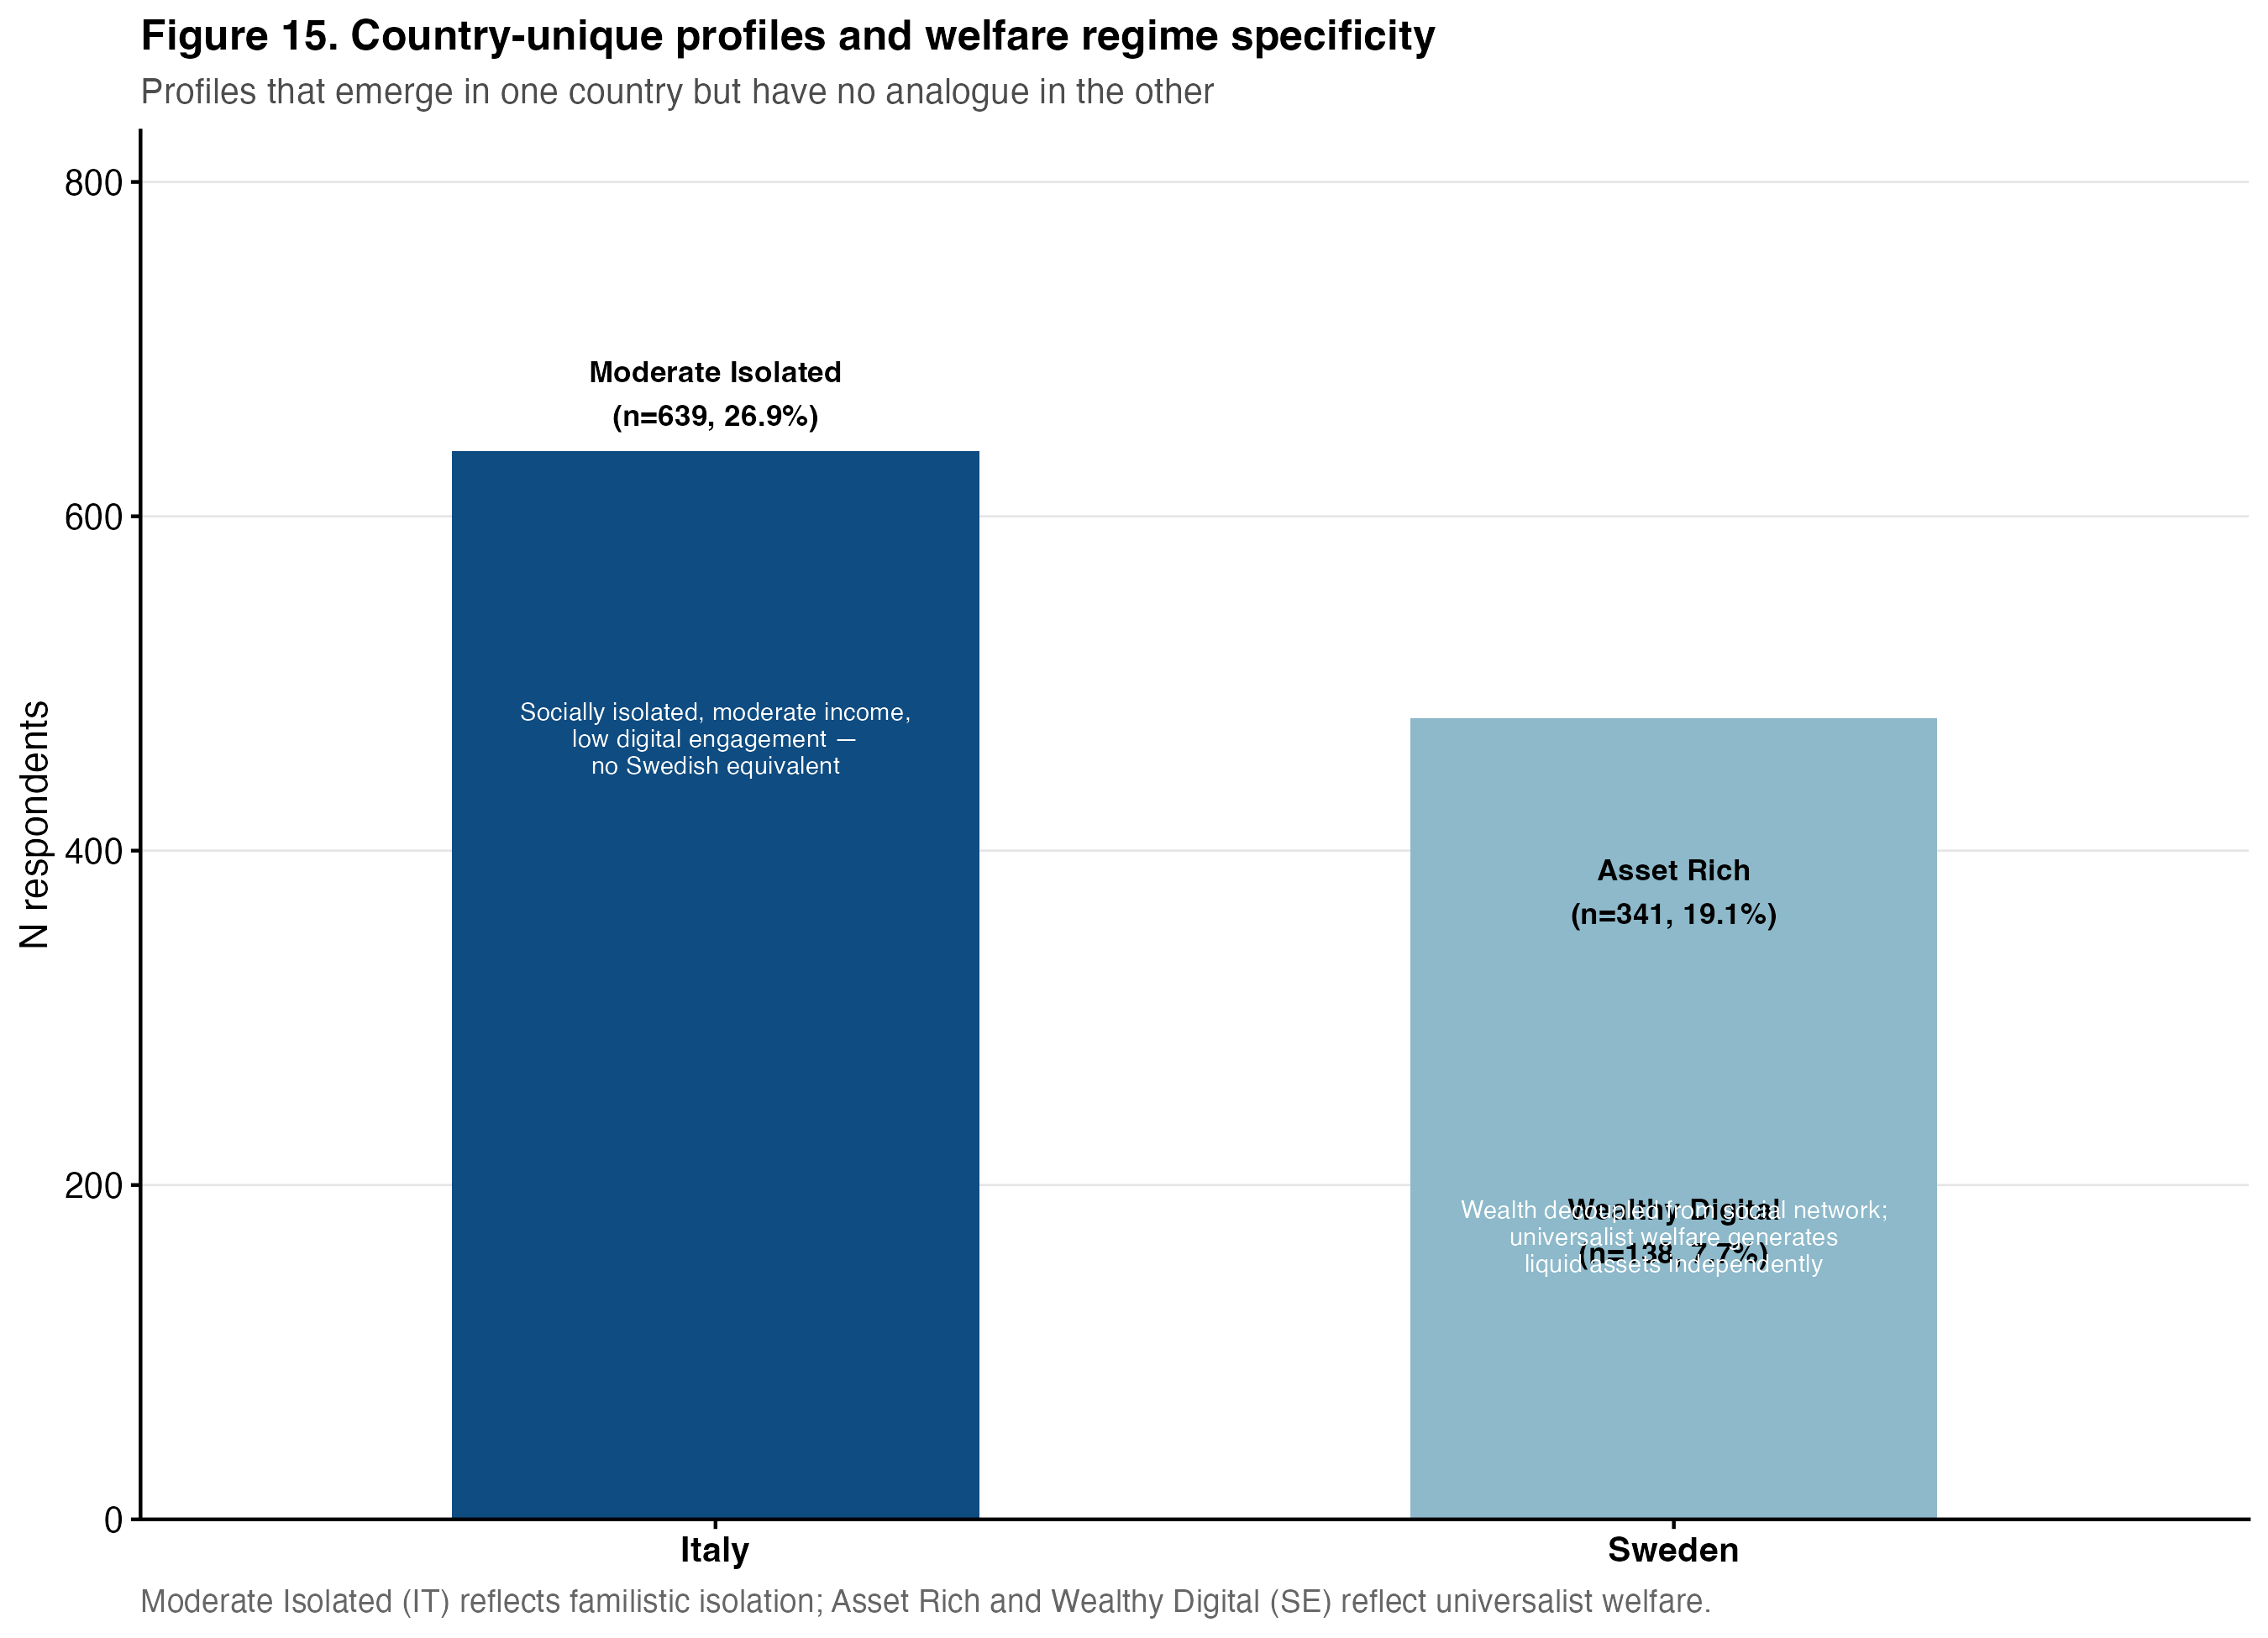
\includegraphics[width=0.78\linewidth]{figures/06_comparison/fig_15_country_unique.png}
  \caption{Welfare-regime-specific profiles in Italy and Sweden. Source: v9 pipeline.}
  \label{fig:ch5-country-unique}
\end{figure}

\section{Pooled latent space}
\label{sec:ch5-pooled}

As an additional check on cross-country commensurability, PCA and factor analysis were re-estimated on the pooled $n = 4{,}165$ sample after joint standardisation. Figure~\ref{fig:ch5-pc-pooled} and Figure~\ref{fig:ch5-fa-pooled} show respondents from both countries in the first principal-component and principal-axis planes respectively. The two country distributions overlap substantially on the second axis but separate on the first --- consistent with a shared latent structure and a country-specific level gradient, i.e.\ the same interpretation supported by Table~\ref{tab:ch5-gap}.

\begin{figure}[ht]
  \centering
  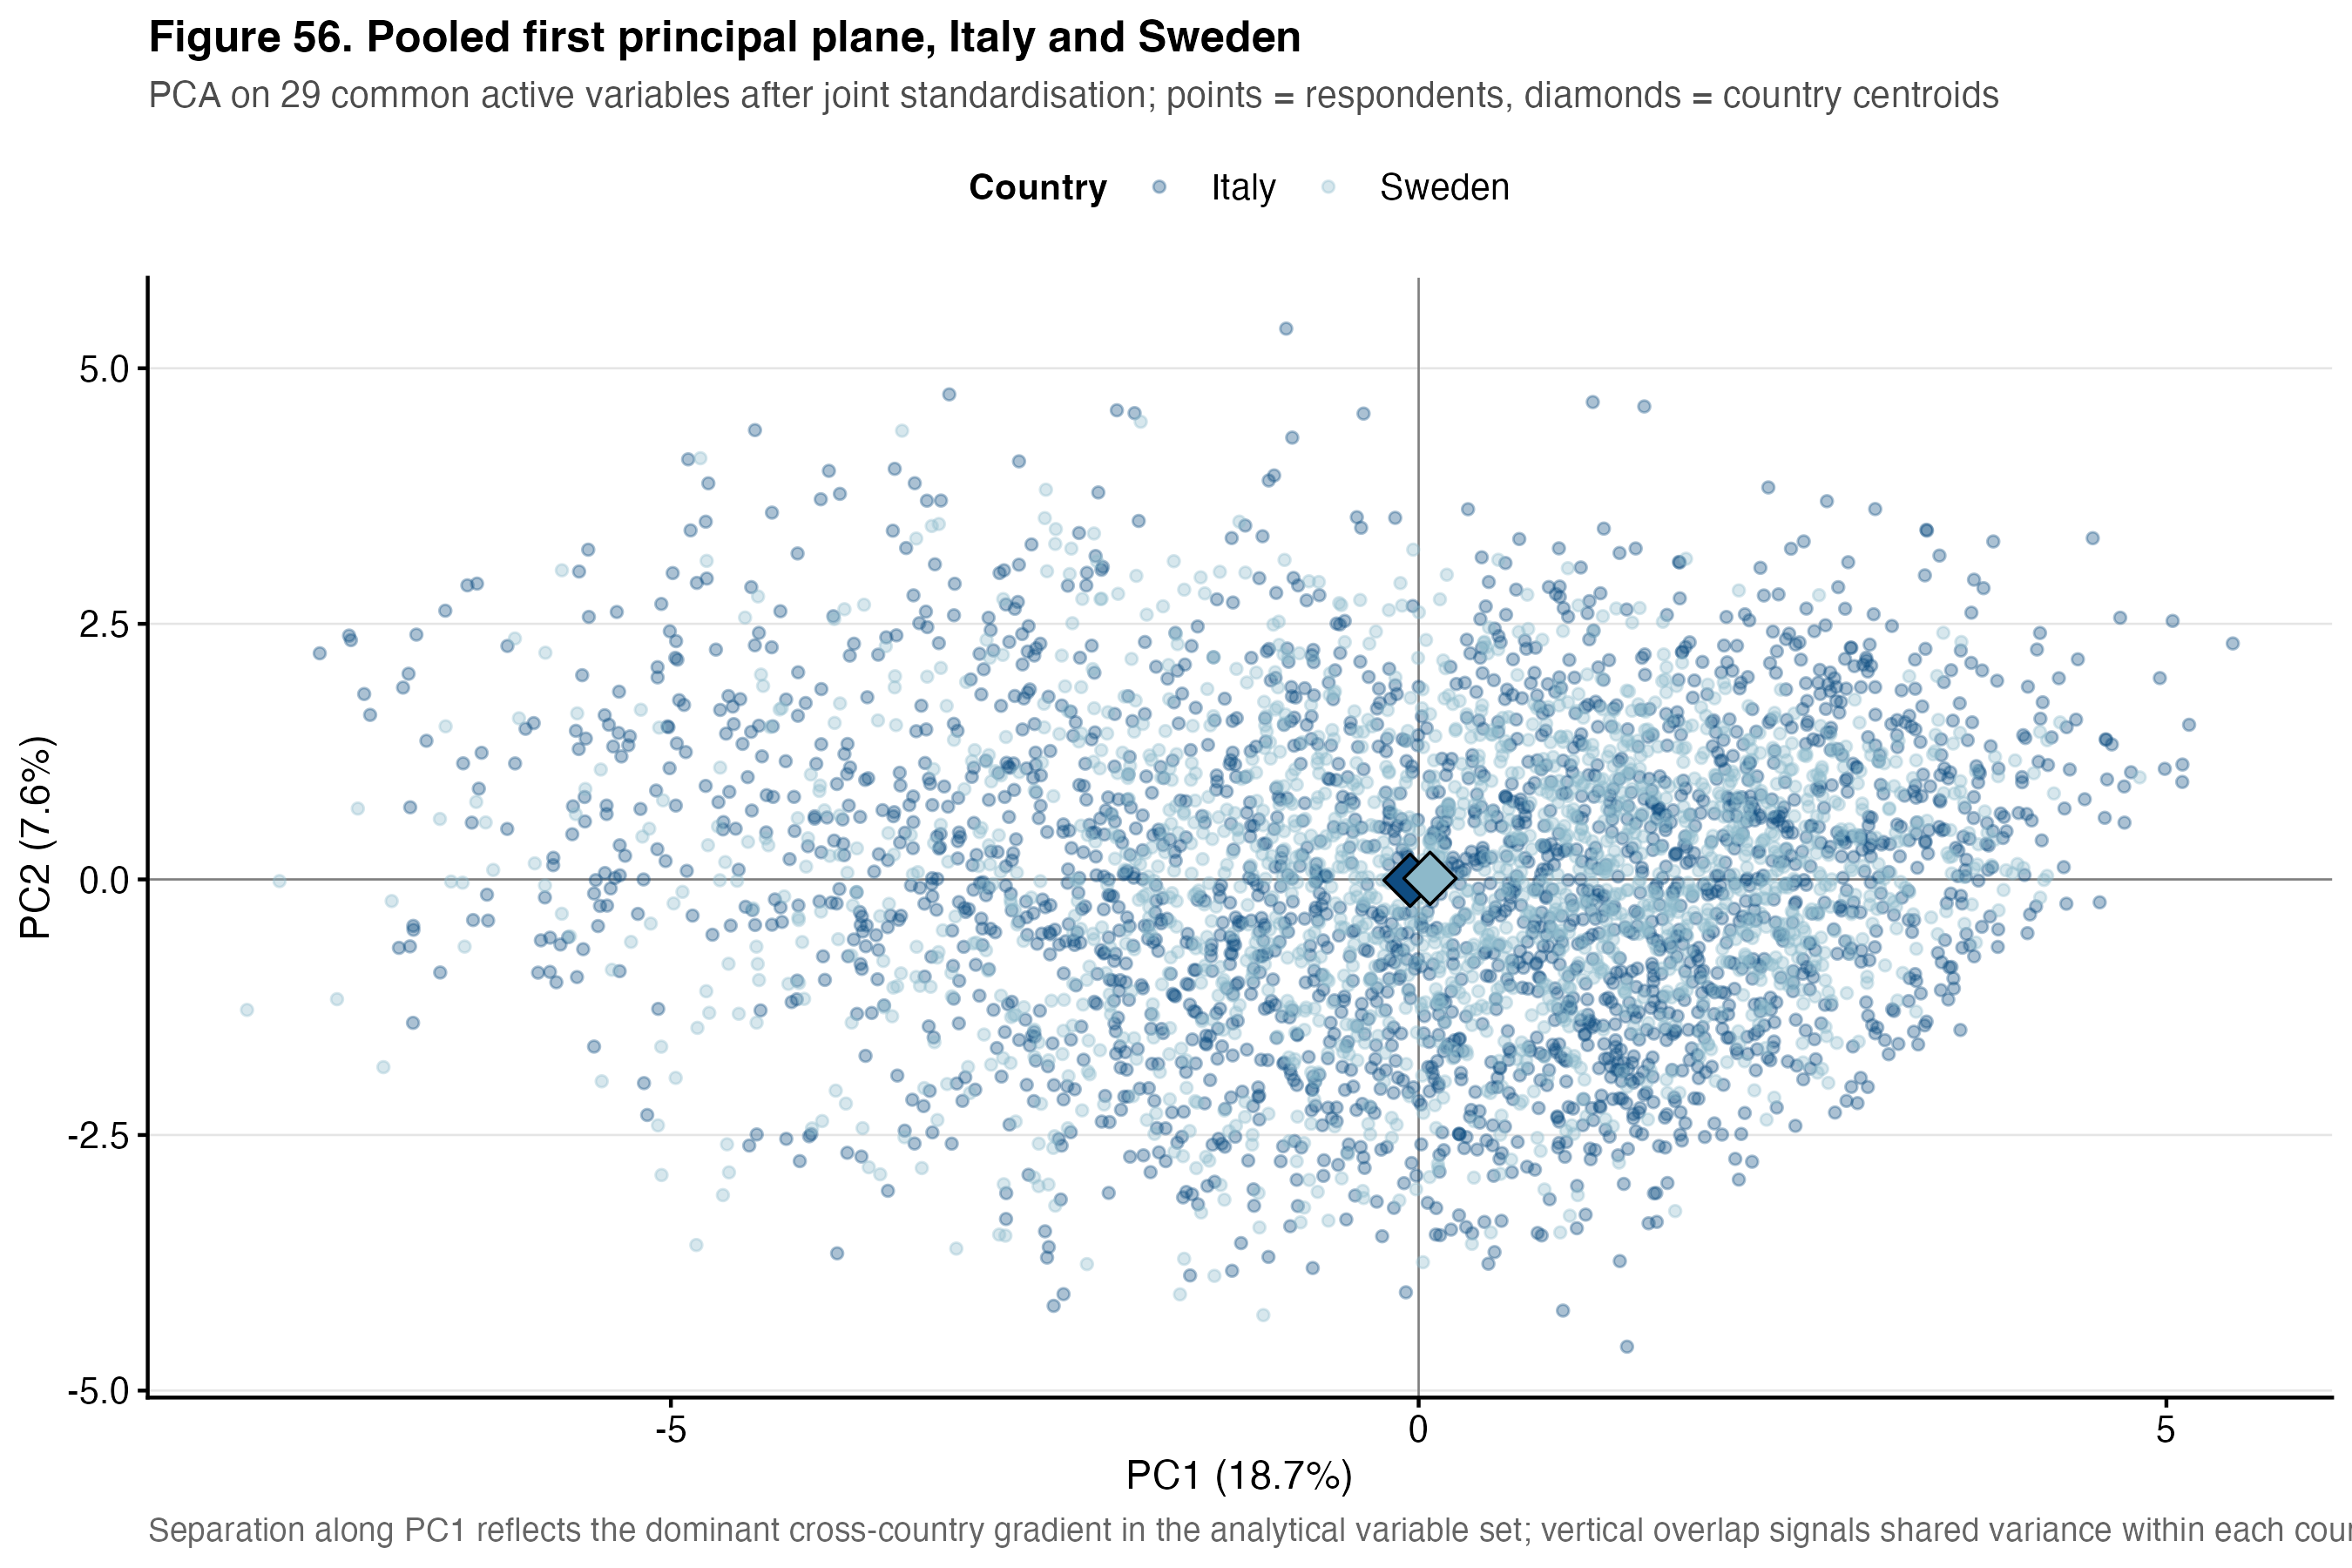
\includegraphics[width=0.85\linewidth]{figures/06_comparison/fig_56_pc_pooled_by_country.png}
  \caption{Respondents in the pooled PC1--PC2 space, coloured by country. Source: v9 pipeline.}
  \label{fig:ch5-pc-pooled}
\end{figure}

\begin{figure}[ht]
  \centering
  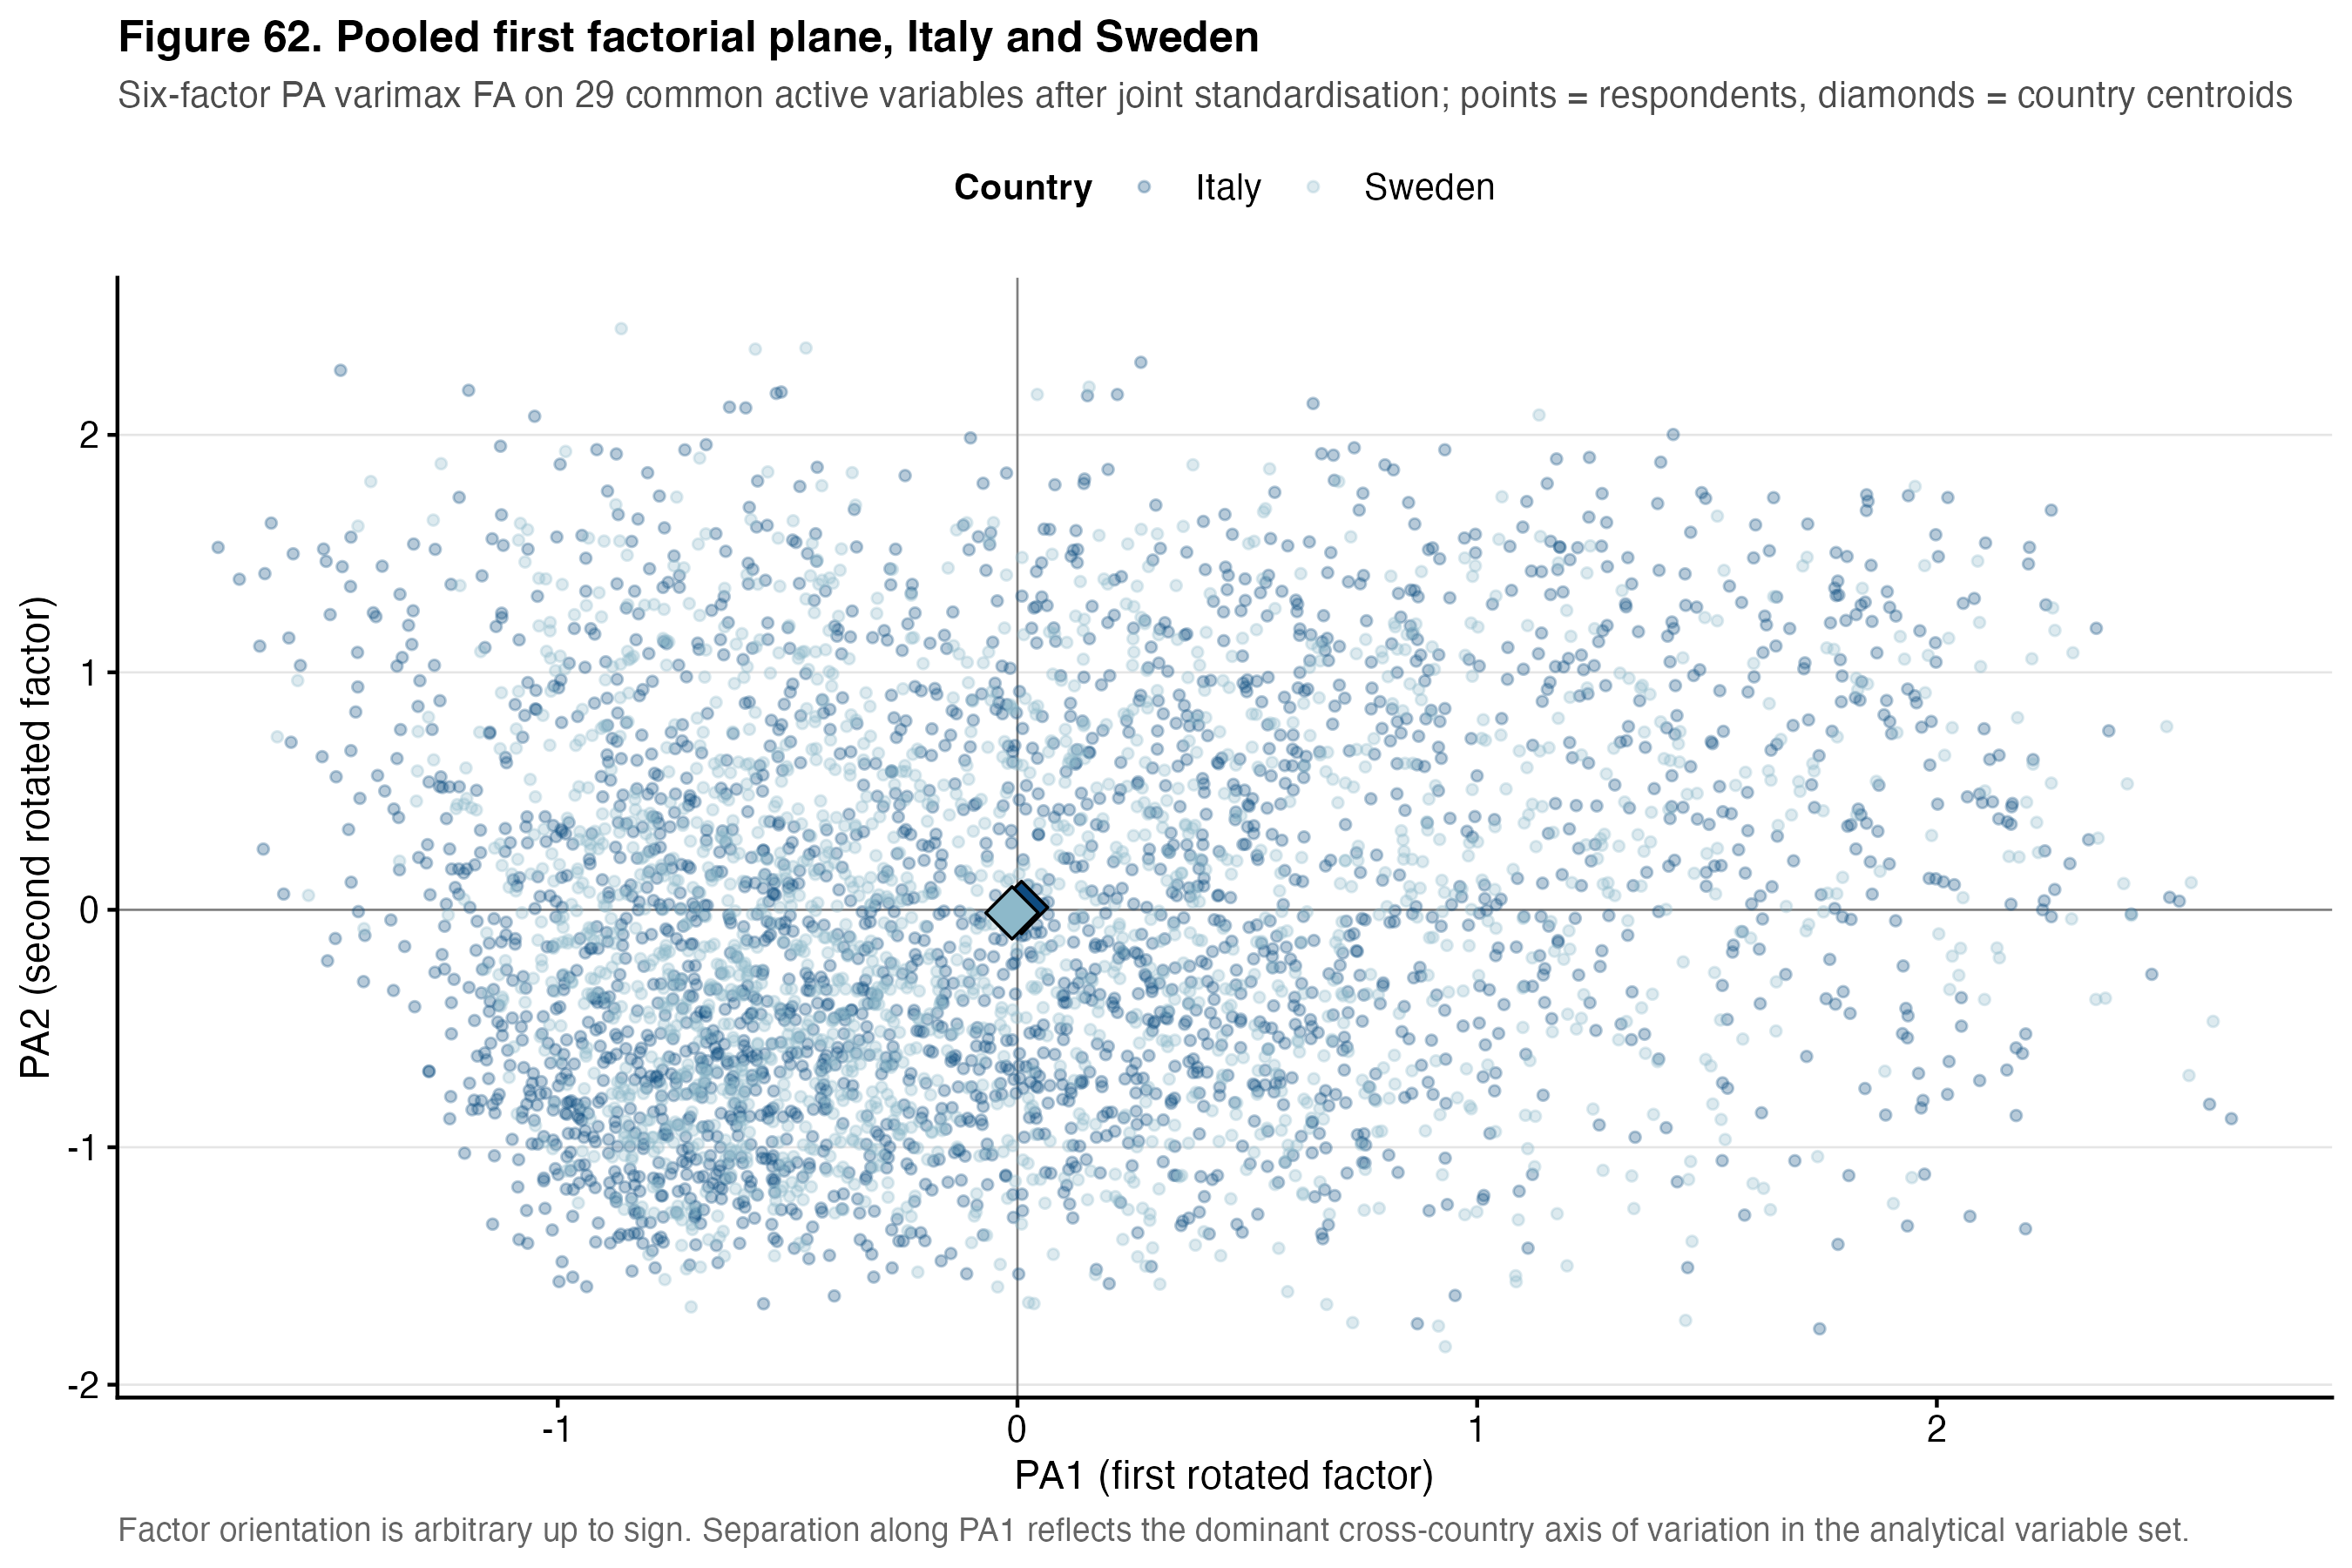
\includegraphics[width=0.85\linewidth]{figures/06_comparison/fig_62_fa_pooled_by_country.png}
  \caption{Respondents in the pooled PA1--PA2 factor-score space, coloured by country. Source: v9 pipeline.}
  \label{fig:ch5-fa-pooled}
\end{figure}

\section{Chapter summary}
\label{sec:ch5-summary}

The same analytical pipeline produces rhyming profile structures in Italy and Sweden, confirming the cross-country usability of the segmentation framework. Within this common structure, Sweden exceeds Italy on every positive indicator of subjective well-being, cognitive function, and digital inclusion, with gaps that are largest for the most vulnerable profiles. Two profiles have no cross-country analogue: the Italian \emph{Moderate Isolated}, whose characterisation prepares the healthcare chapter that follows, and the Swedish \emph{Asset Rich} and \emph{Wealthy Digital} types, interpretable as welfare-regime-specific signatures of the universalist model.

\chapter{Robustness and sensitivity}
\label{ch:ch6}

This chapter assesses the robustness of the profile structure reported in Chapters~\ref{ch:ch4} and~\ref{ch:ch5} along five independent lines. Section~\ref{sec:ch6-algorithms} compares K-means against three agglomerative alternatives. Section~\ref{sec:ch6-duda-hart} reports the Duda--Hart cut-off diagnostics that validate $k = 5$ for Italy and $k = 6$ for Sweden. Section~\ref{sec:ch6-kmeans-lca} compares the K-means assignments with those produced by a Latent Class Analysis. Section~\ref{sec:ch6-fa-stability} evaluates the stability of the factor solution across countries. Section~\ref{sec:ch6-subjective} is the sensitivity analysis that tests the analytical innovation of the thesis: removing the subjective block from the clustering input.

Table~\ref{tab:ch6-profile-sizes} cross-references the profile sizes used throughout the thesis. The Italian total ($n = 2{,}378$) and the Swedish total ($n = 1{,}787$) correspond to the analytical samples after the Mahalanobis screen described in Section~\ref{sec:ch3-sample}.

\begin{table}[ht]
  \centering
  \caption{Profile sizes used throughout the thesis.}
  \label{tab:ch6-profile-sizes}
  \small
  \begin{tabular}{@{}lrr@{}}
    \toprule
    \textbf{Profile} & \textbf{Italy} & \textbf{Sweden}\\
    \midrule
    Fragile Resigned      & 315  & ---  \\
    Fragile Depressed     & 636  & ---  \\
    Moderate Isolated     & 639  & ---  \\
    Traditional Social    & 184  & ---  \\
    Connected Active      & 604  & ---  \\
    \midrule
    Fragile               & ---  & 206  \\
    Social Decline        & ---  & 149  \\
    Moderate              & ---  & 417  \\
    Asset Rich            & ---  & 341  \\
    Wealthy Digital       & ---  & 138  \\
    Connected Wealthy     & ---  & 536  \\
    \midrule
    \textbf{Total}        & \textbf{2{,}378} & \textbf{1{,}787}\\
    \bottomrule
  \end{tabular}
\end{table}

\section{Cluster quality under alternative algorithms}
\label{sec:ch6-algorithms}

The choice of K-means over hierarchical alternatives was motivated in Section~\ref{sec:ch3-kmeans} on theoretical grounds. Figures~\ref{fig:ch6-multi-alg-italy} and~\ref{fig:ch6-multi-alg-sweden} confirm that motivation empirically. Across $k = 2,\ldots,12$ and across the four algorithms considered (K-means, Ward, complete linkage, average linkage), K-means attains uniformly higher within-cluster $R^{2}$ and silhouette than its agglomerative competitors in both countries. Ward linkage is competitive only on the Dunn index, which penalises cluster elongation differently and is known to favour ellipsoidal shapes.

\begin{figure}[ht]
  \centering
  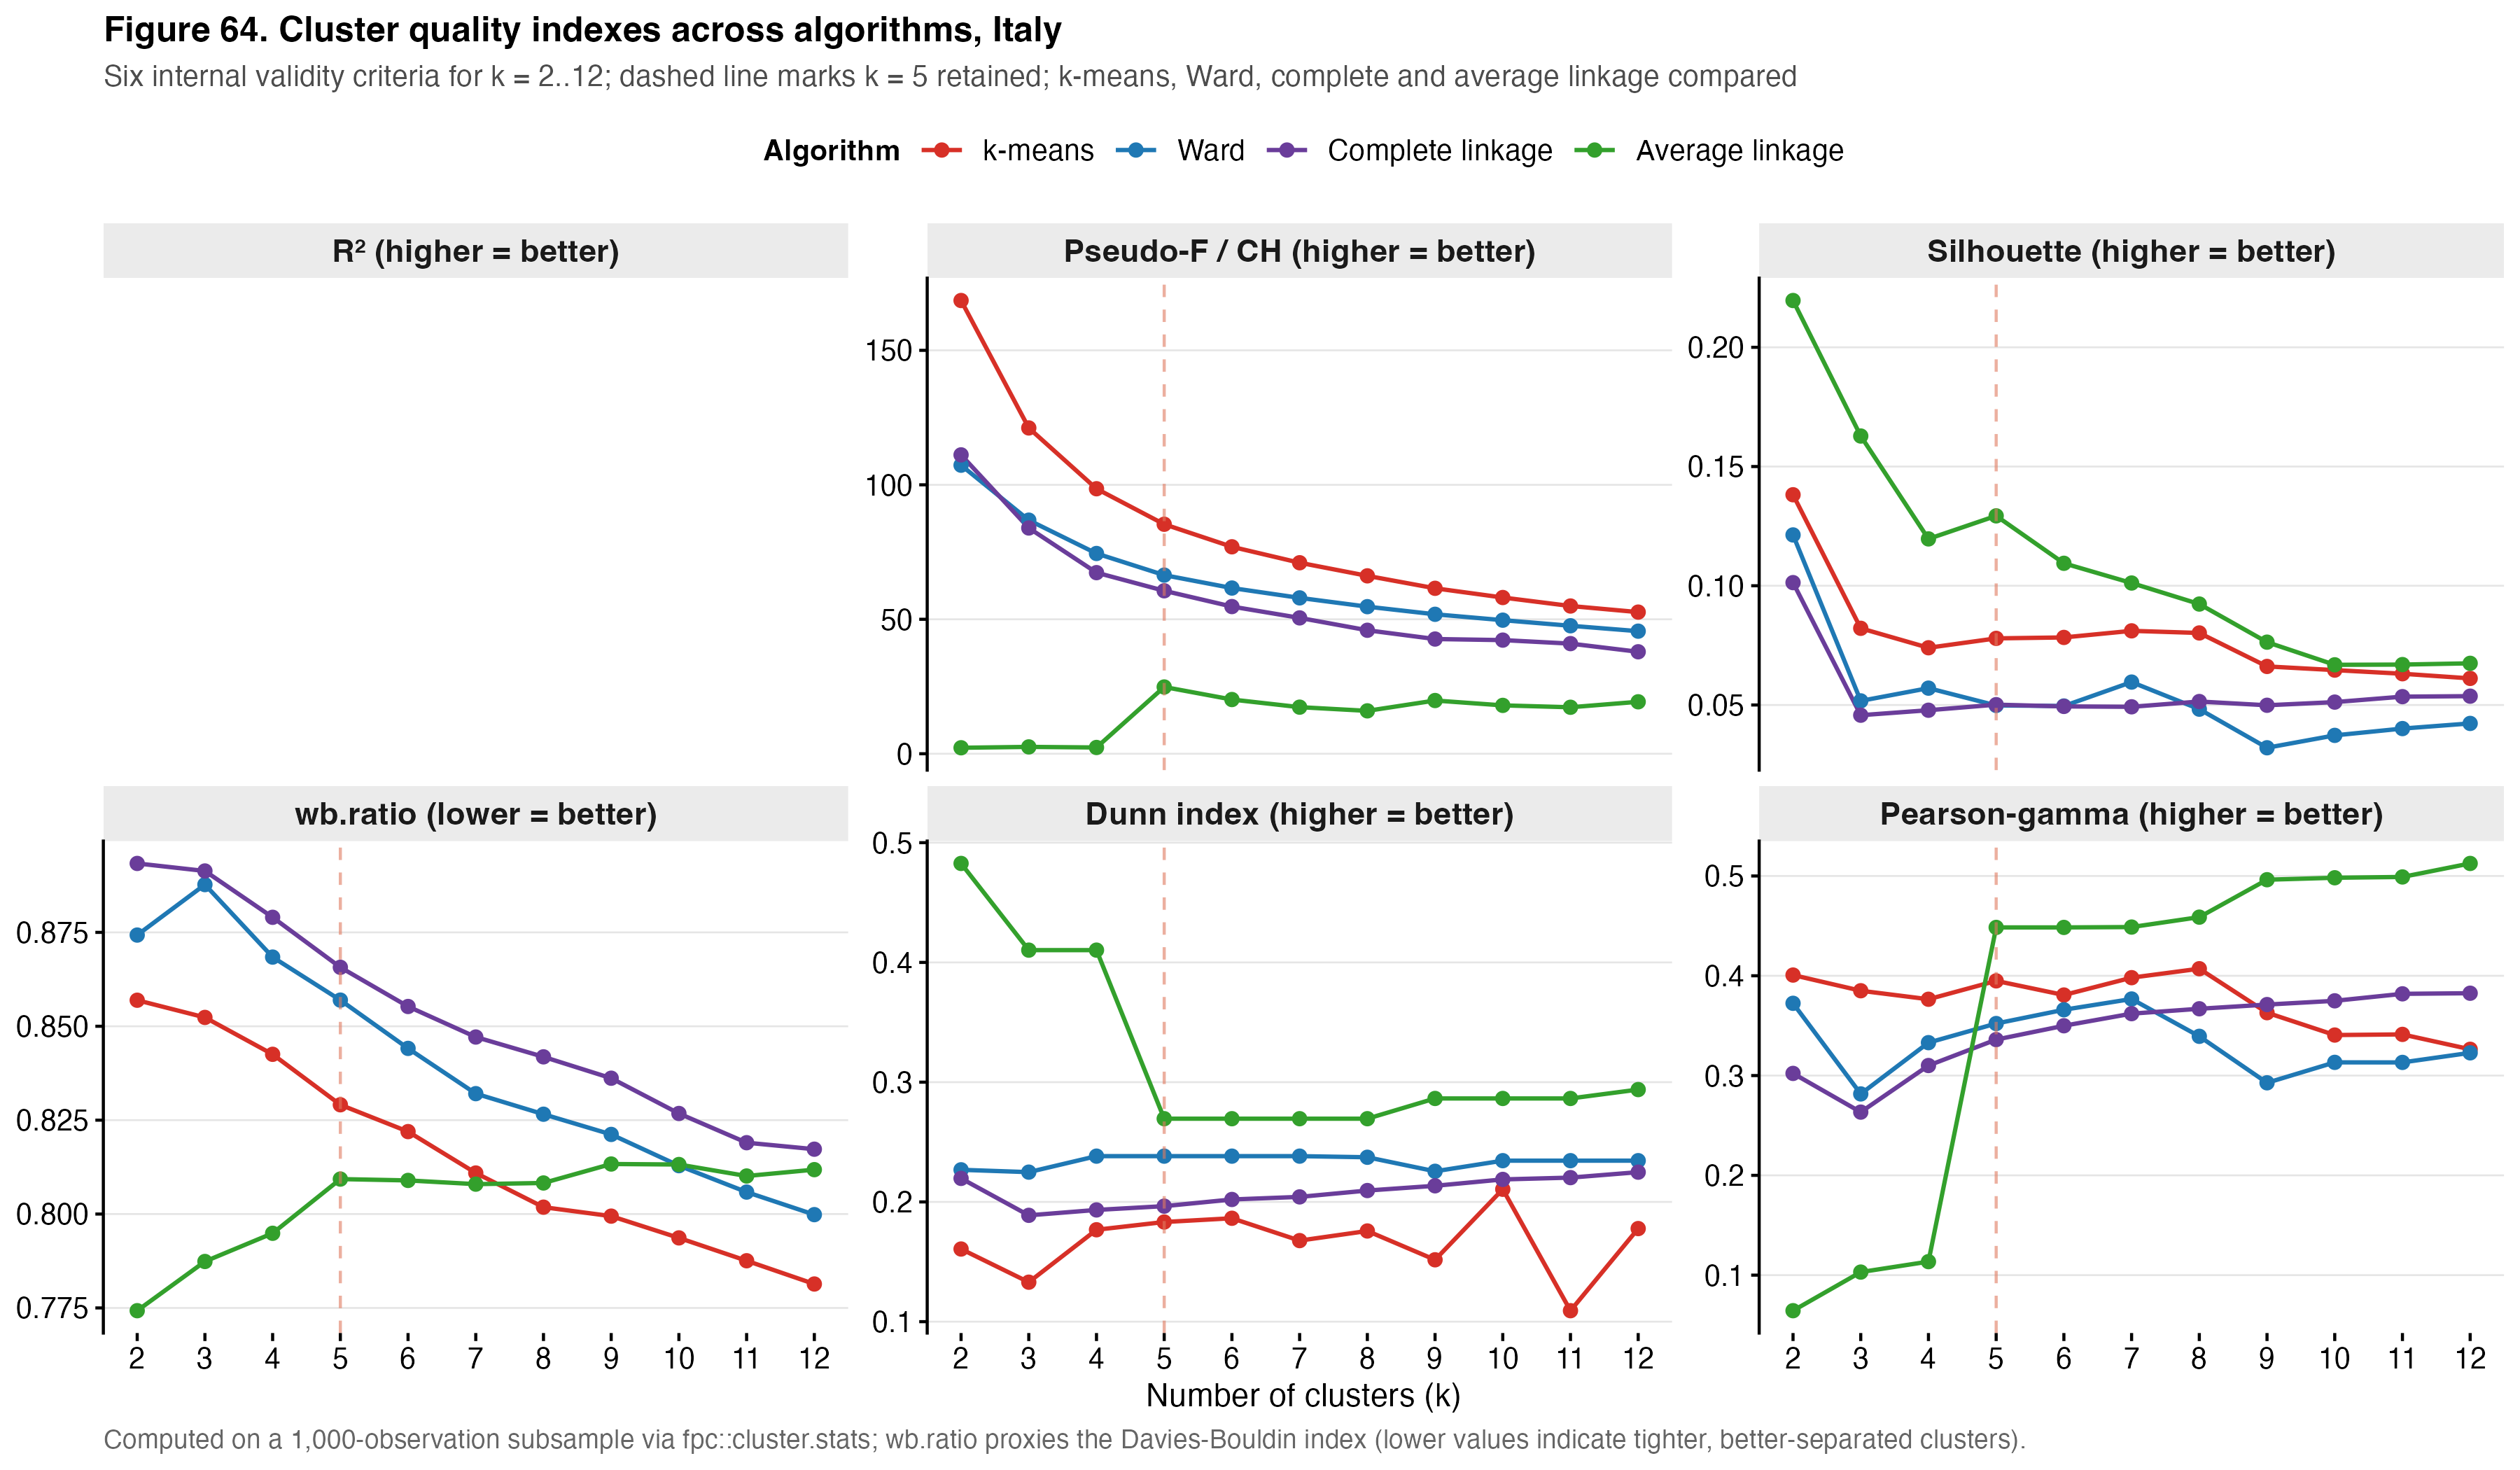
\includegraphics[width=0.92\linewidth]{figures/07_robustness/fig_64_cluster_quality_multi_alg_italy.png}
  \caption{Italy: six internal validity indexes for $k = 2,\ldots,12$ across four clustering algorithms. Source: v9 pipeline.}
  \label{fig:ch6-multi-alg-italy}
\end{figure}

\begin{figure}[ht]
  \centering
  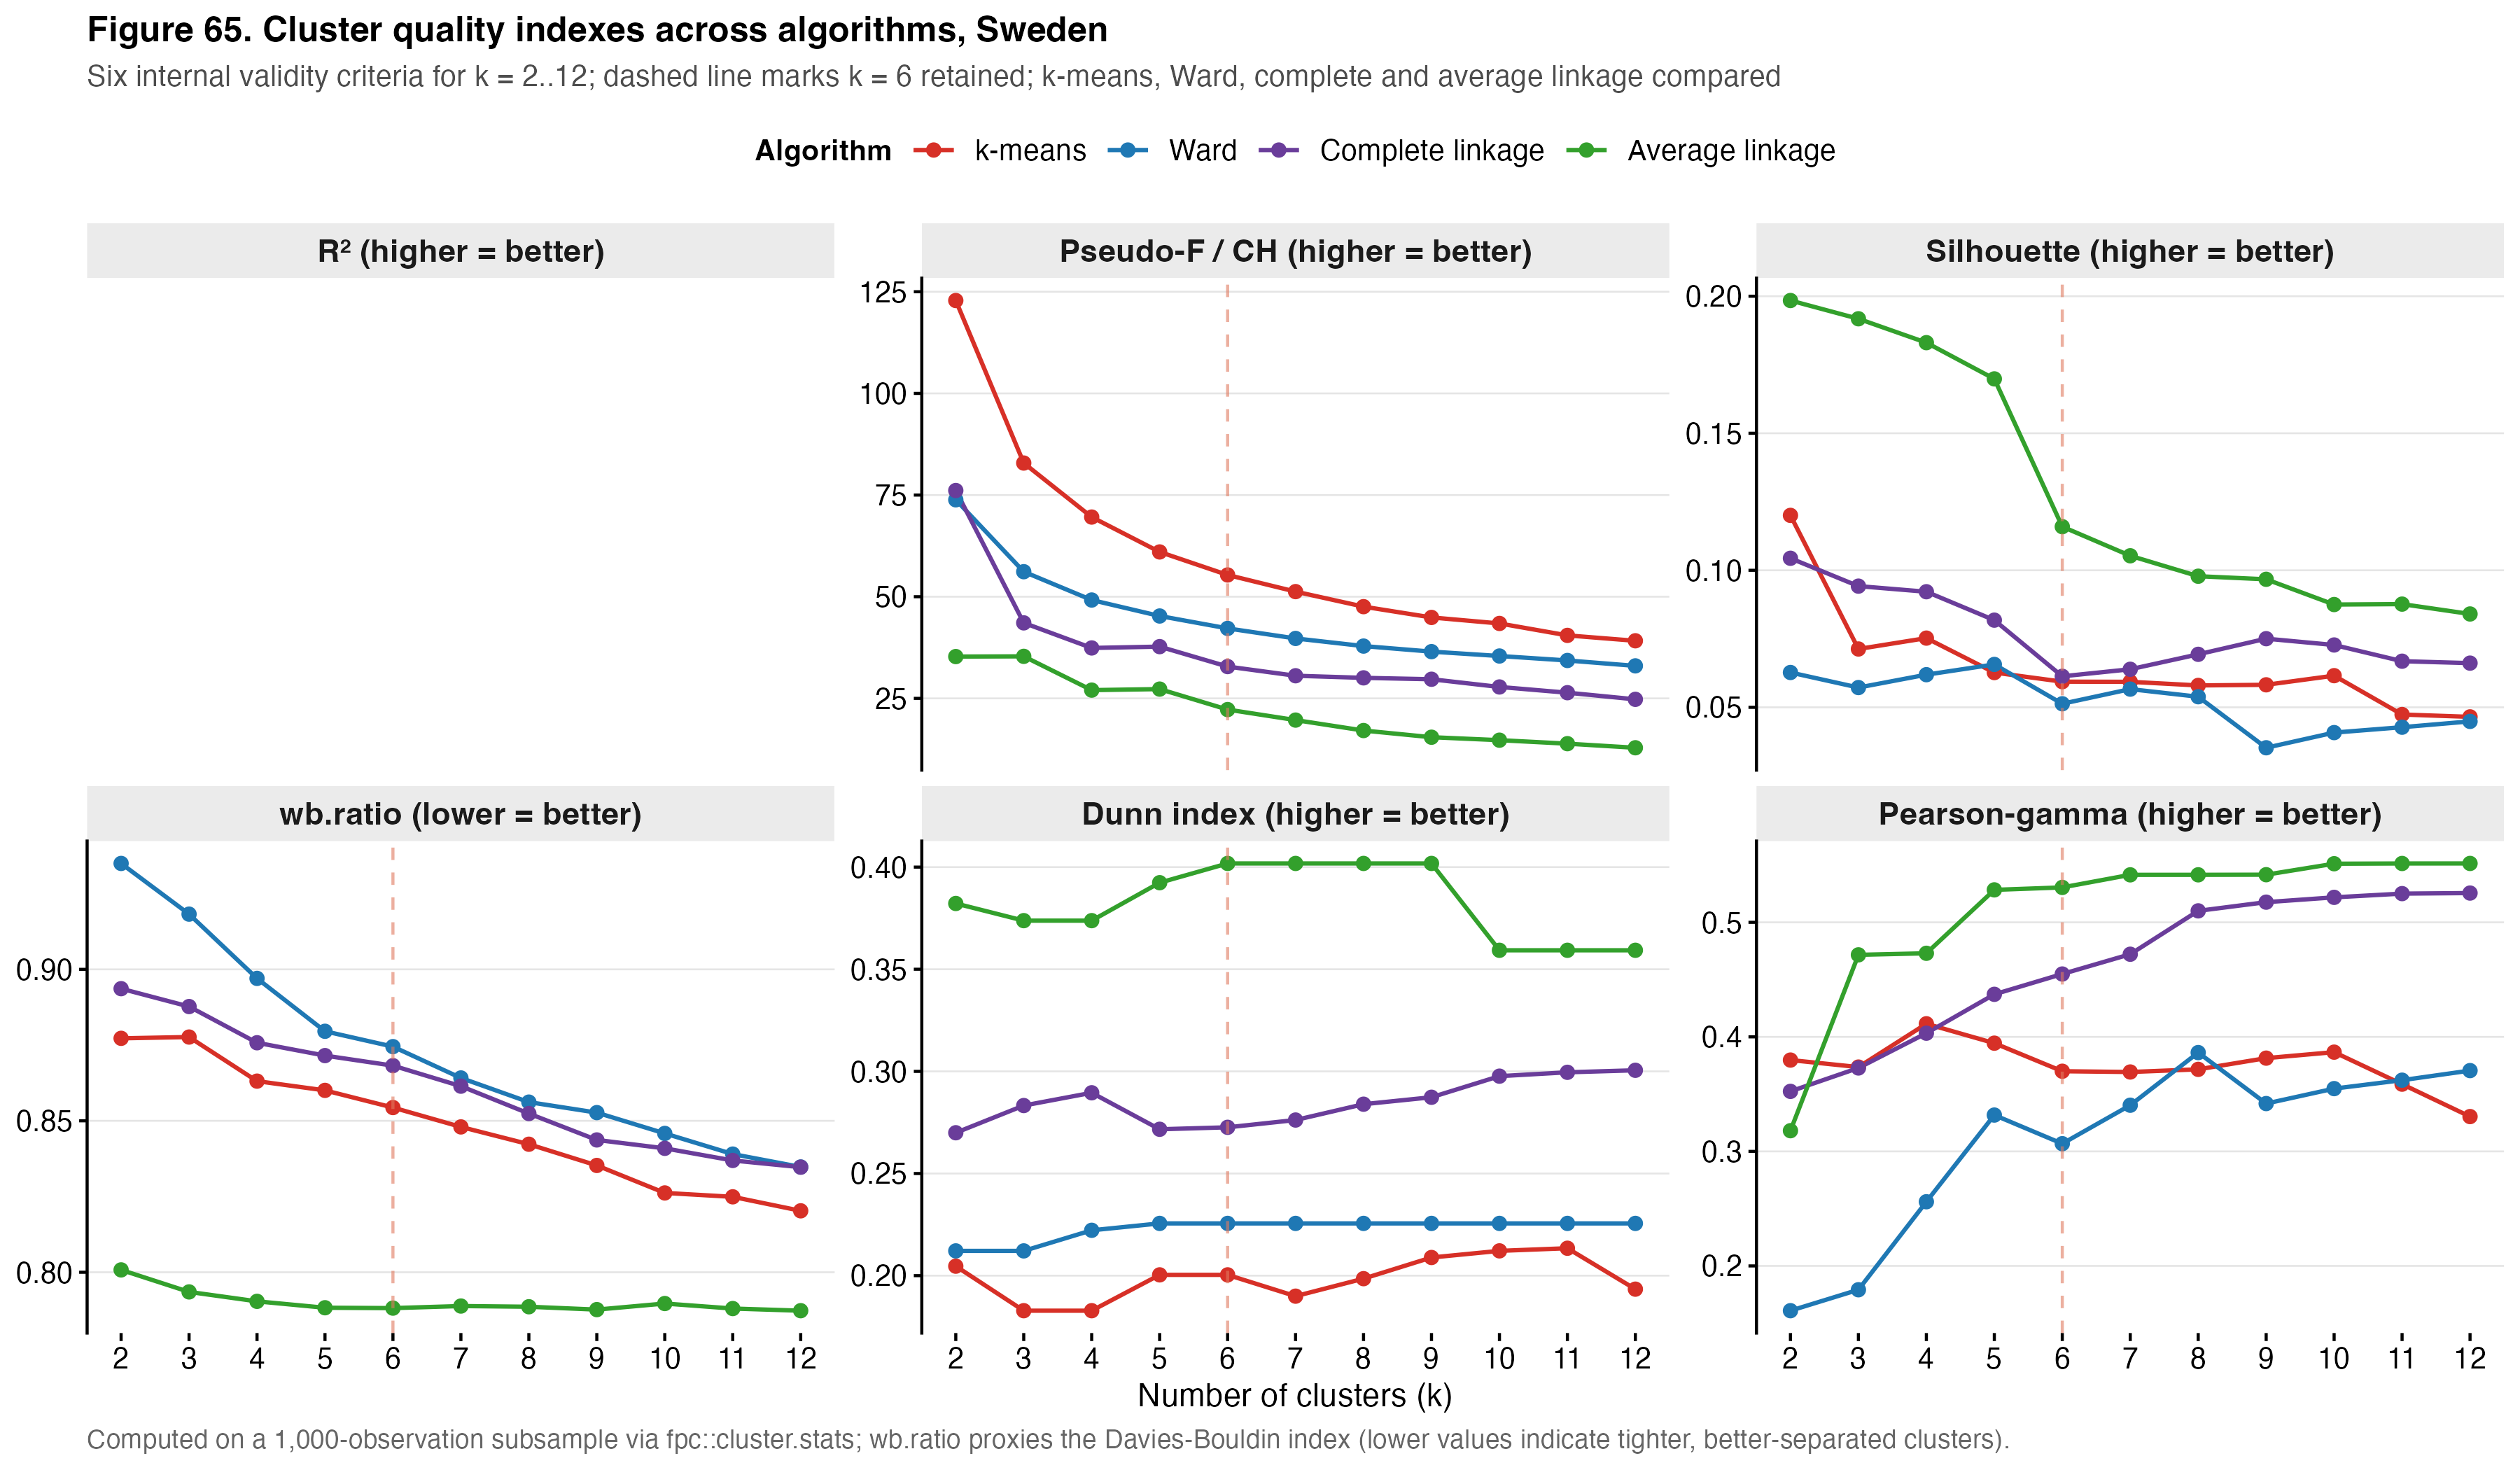
\includegraphics[width=0.92\linewidth]{figures/07_robustness/fig_65_cluster_quality_multi_alg_sweden.png}
  \caption{Sweden: six internal validity indexes for $k = 2,\ldots,12$ across four clustering algorithms. Source: v9 pipeline.}
  \label{fig:ch6-multi-alg-sweden}
\end{figure}

Figures~\ref{fig:ch6-varspec-italy} and~\ref{fig:ch6-varspec-sweden} report, variable by variable, the within-cluster $R^{2}$ attained by each algorithm at each $k$. Two interpretive patterns emerge. First, a small group of indicators --- notably \emph{bmi} and \emph{received help} (\emph{sp002\_}) --- carries no clustering signal under any method at any $k$; these variables are retained because the thesis's methodological choice is to refrain from ad-hoc variable pruning, but the reader is alerted that their contribution to the partition is nil. Second, the bulk of the indicators saturate their within-cluster $R^{2}$ precisely in the $k = 5,\ldots,6$ range, which converges with the empirical and substantive choice of $k = 5$ for Italy and $k = 6$ for Sweden.

\begin{figure}[ht]
  \centering
  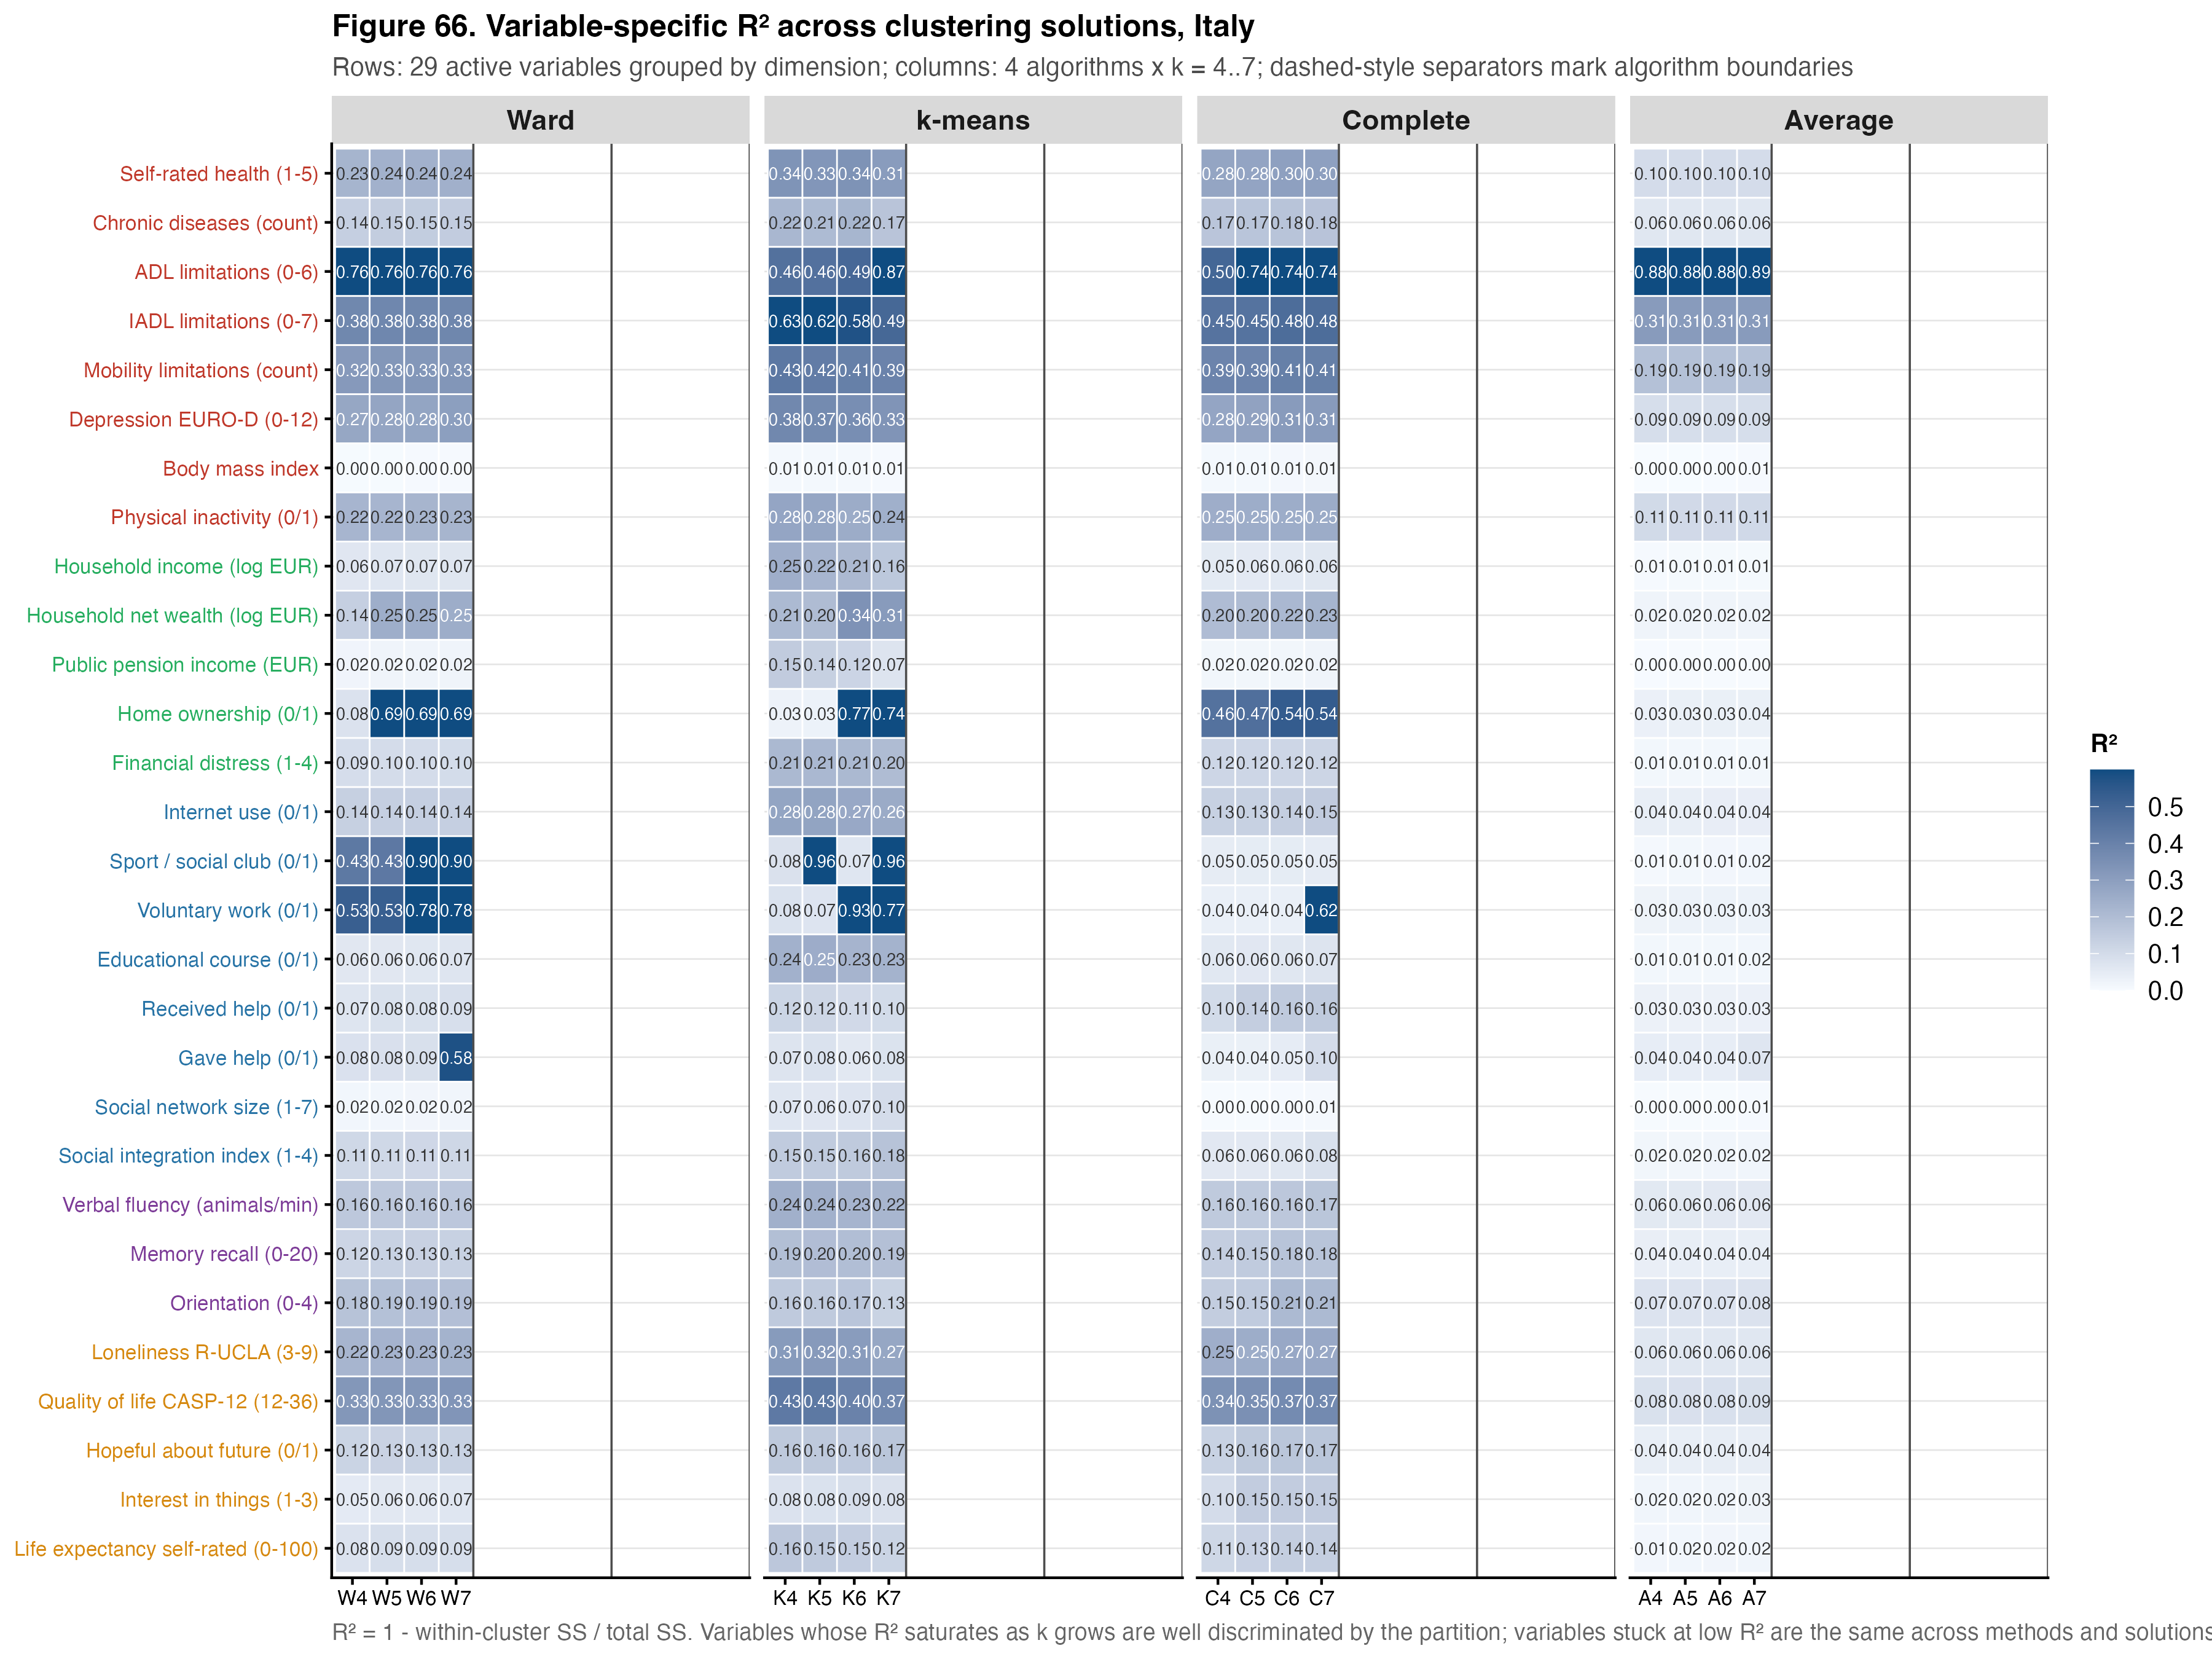
\includegraphics[width=0.92\linewidth]{figures/07_robustness/fig_66_varspec_r2_italy.png}
  \caption{Italy: variable-specific within-cluster $R^{2}$ across clustering solutions. Source: v9 pipeline.}
  \label{fig:ch6-varspec-italy}
\end{figure}

\begin{figure}[ht]
  \centering
  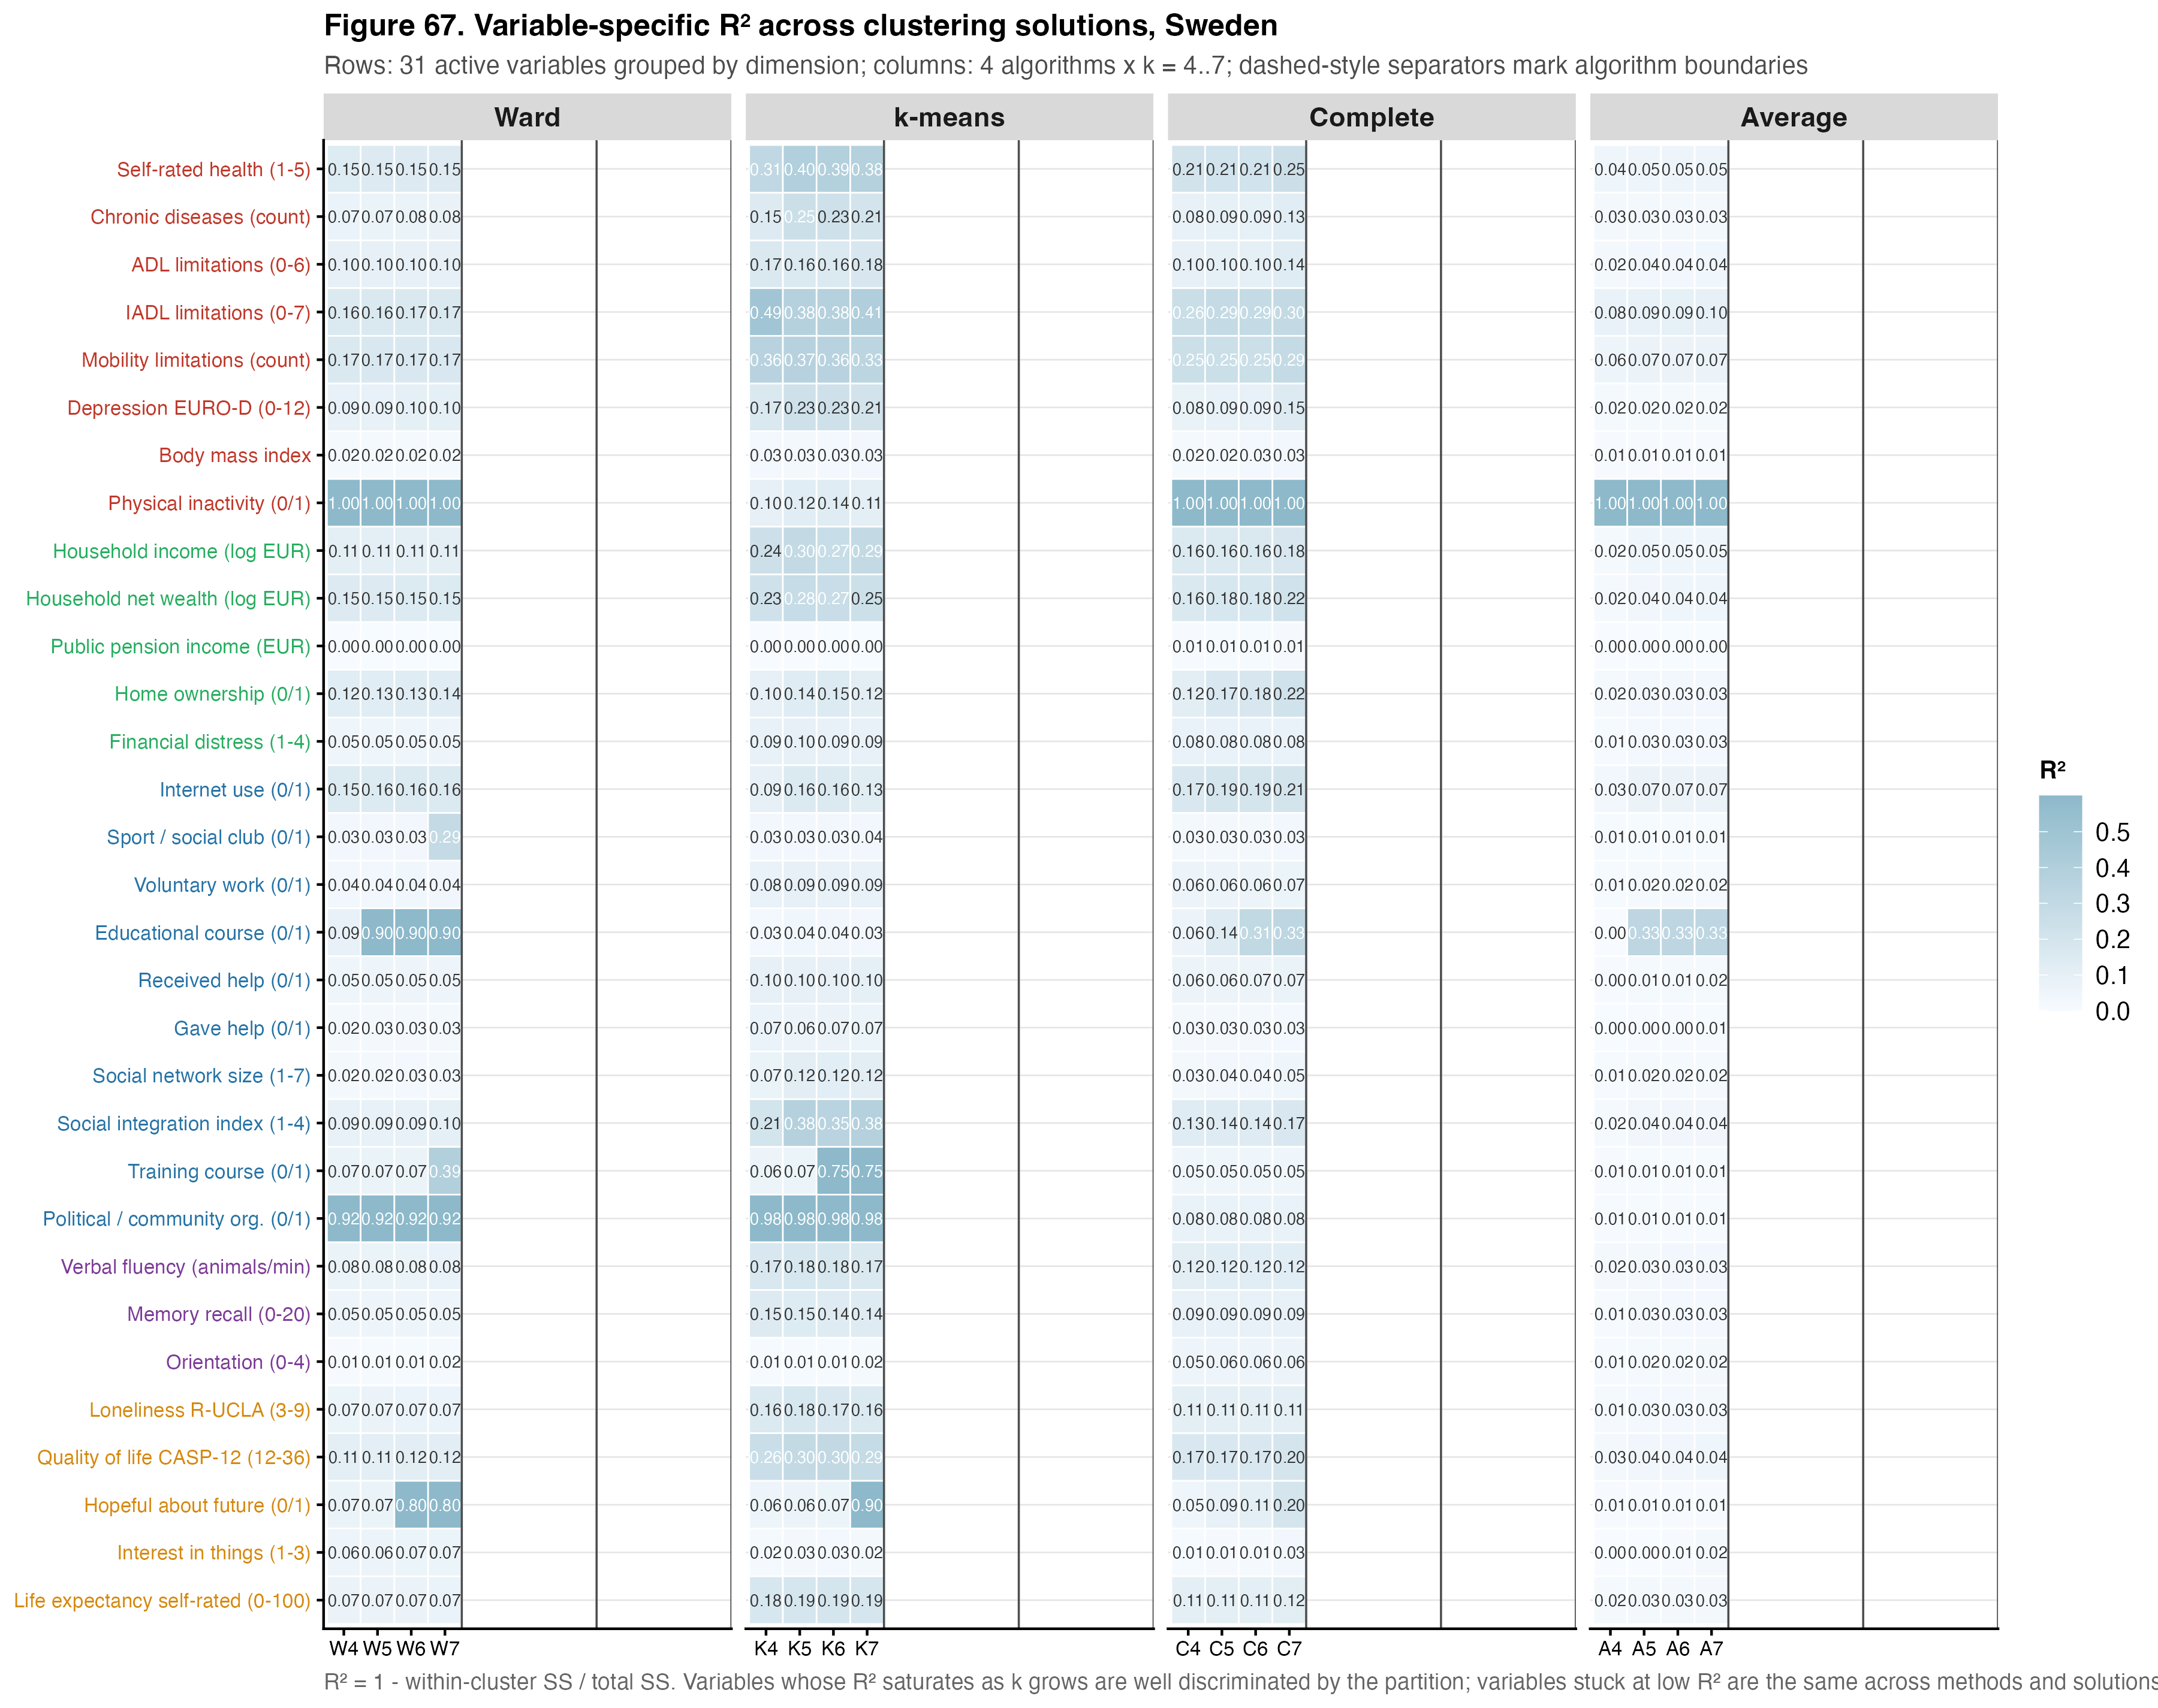
\includegraphics[width=0.92\linewidth]{figures/07_robustness/fig_67_varspec_r2_sweden.png}
  \caption{Sweden: variable-specific within-cluster $R^{2}$ across clustering solutions. Source: v9 pipeline.}
  \label{fig:ch6-varspec-sweden}
\end{figure}

\section{Hierarchical cut-off diagnostics (Duda--Hart)}
\label{sec:ch6-duda-hart}

Figures~\ref{fig:ch6-sprt2-italy} and~\ref{fig:ch6-sprt2-sweden} report the semi-partial $R^{2}$ (SPR$^{2}$) and the Pseudo-$T^{2}$ (PST$^{2}$) diagnostics of Duda and Hart for the three agglomerative linkages across $k = 2,\ldots,12$. These curves identify the "merge cost" at each level of the hierarchy: a peak in PST$^{2}$ or a sharp jump in SPR$^{2}$ at $k = k^{*}$ signals that collapsing two clusters at that level destroys a well-separated group, which is the classical criterion for cutting the tree at $k^{*}$.

\begin{figure}[ht]
  \centering
  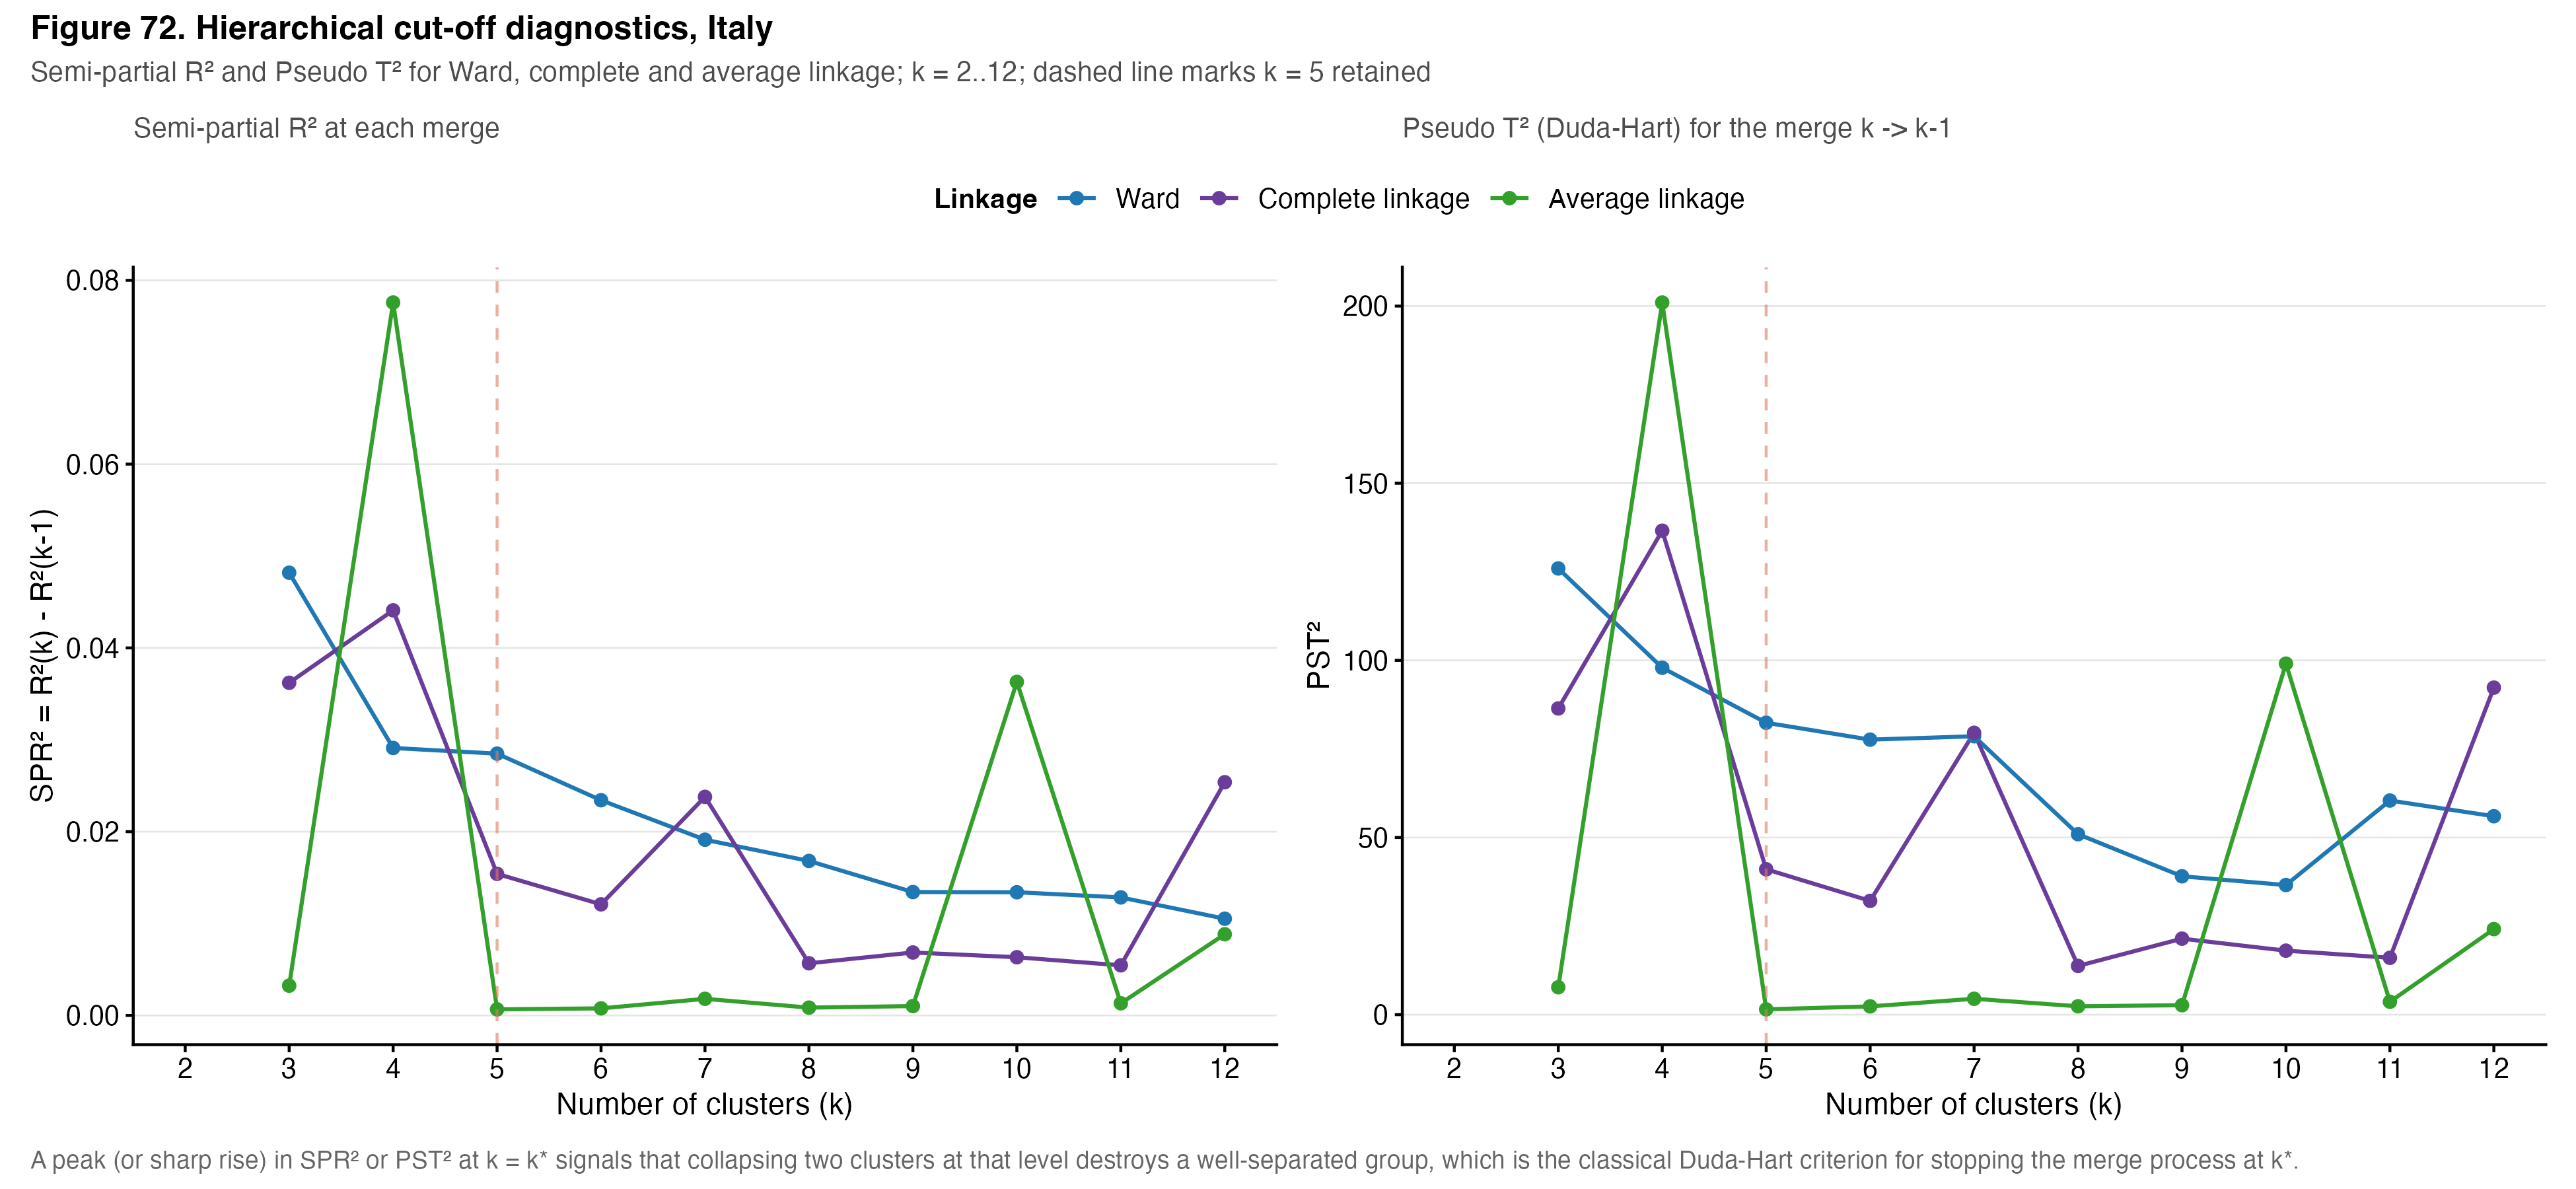
\includegraphics[width=0.92\linewidth]{figures/08_appendix/fig_72_spr2_pst2_italy.png}
  \caption{Italy: semi-partial $R^{2}$ and Pseudo-$T^{2}$ for Ward, complete, and average linkage. Dashed line marks $k = 5$. Source: v9 pipeline.}
  \label{fig:ch6-sprt2-italy}
\end{figure}

\begin{figure}[ht]
  \centering
  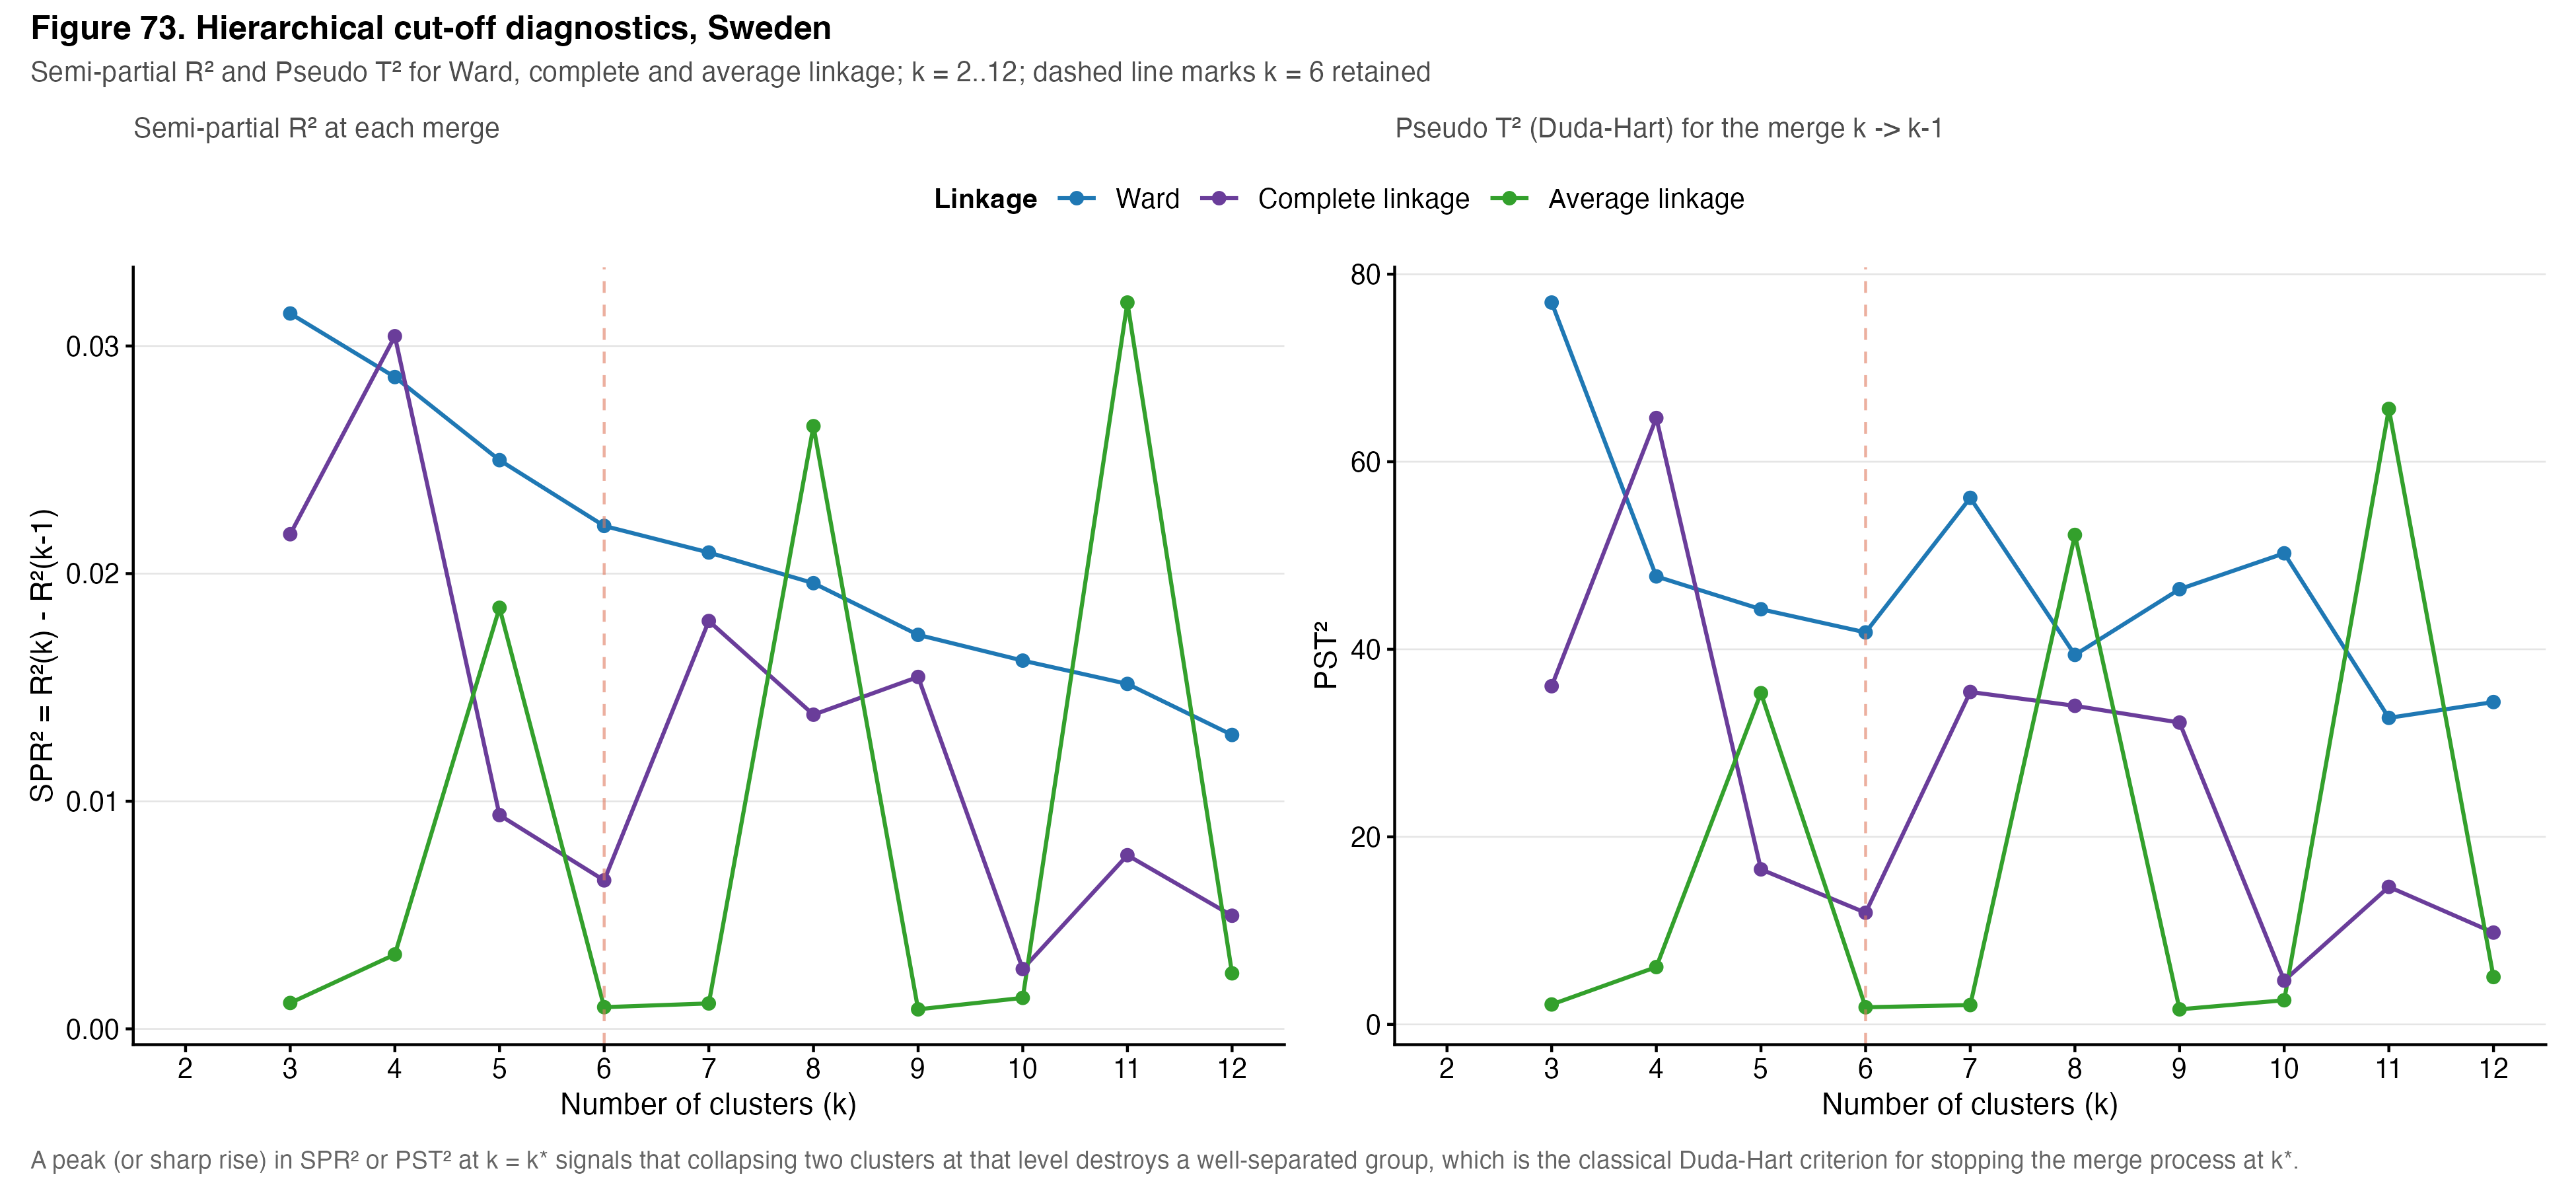
\includegraphics[width=0.92\linewidth]{figures/08_appendix/fig_73_spr2_pst2_sweden.png}
  \caption{Sweden: semi-partial $R^{2}$ and Pseudo-$T^{2}$ for Ward, complete, and average linkage. Dashed line marks $k = 6$. Source: v9 pipeline.}
  \label{fig:ch6-sprt2-sweden}
\end{figure}

The peaks of PST$^{2}$ for Ward linkage fall at $k = 5$ in Italy and at $k = 6$ in Sweden, independently corroborating the cut-off chosen for the K-means solution. On average and complete linkage the peaks are less sharp, consistent with the known tendency of those methods to produce shallower dendrogram structures under mixed-scale data.

\section{Convergence between K-means and Latent Class Analysis}
\label{sec:ch6-kmeans-lca}

Latent Class Analysis provides a probabilistic alternative to the distance-based K-means. Convergence between the two is the most stringent internal robustness check, because the two methods rest on different theoretical premises: K-means minimises the within-cluster sum of squares under a hard-assignment, equal-variance Gaussian assumption, while LCA models the joint distribution of the (discretised) indicators as a mixture of multinomials and yields posterior class probabilities.

Figures~\ref{fig:ch6-lca-fit}, \ref{fig:ch6-lca-confusion} and~\ref{fig:ch6-convergence} summarise the result. The BIC of LCA is minimised at $k = 6$ for both countries, matching the $k$ retained in the K-means stage. Normalised entropy of the LCA posterior is $0.83$ in Italy and in Sweden, above the conventional 0.80 threshold for adequate classification quality. The confusion matrices between K-means and the modal LCA class show that the majority of respondents land in the same class under both methods.

\begin{figure}[ht]
  \centering
  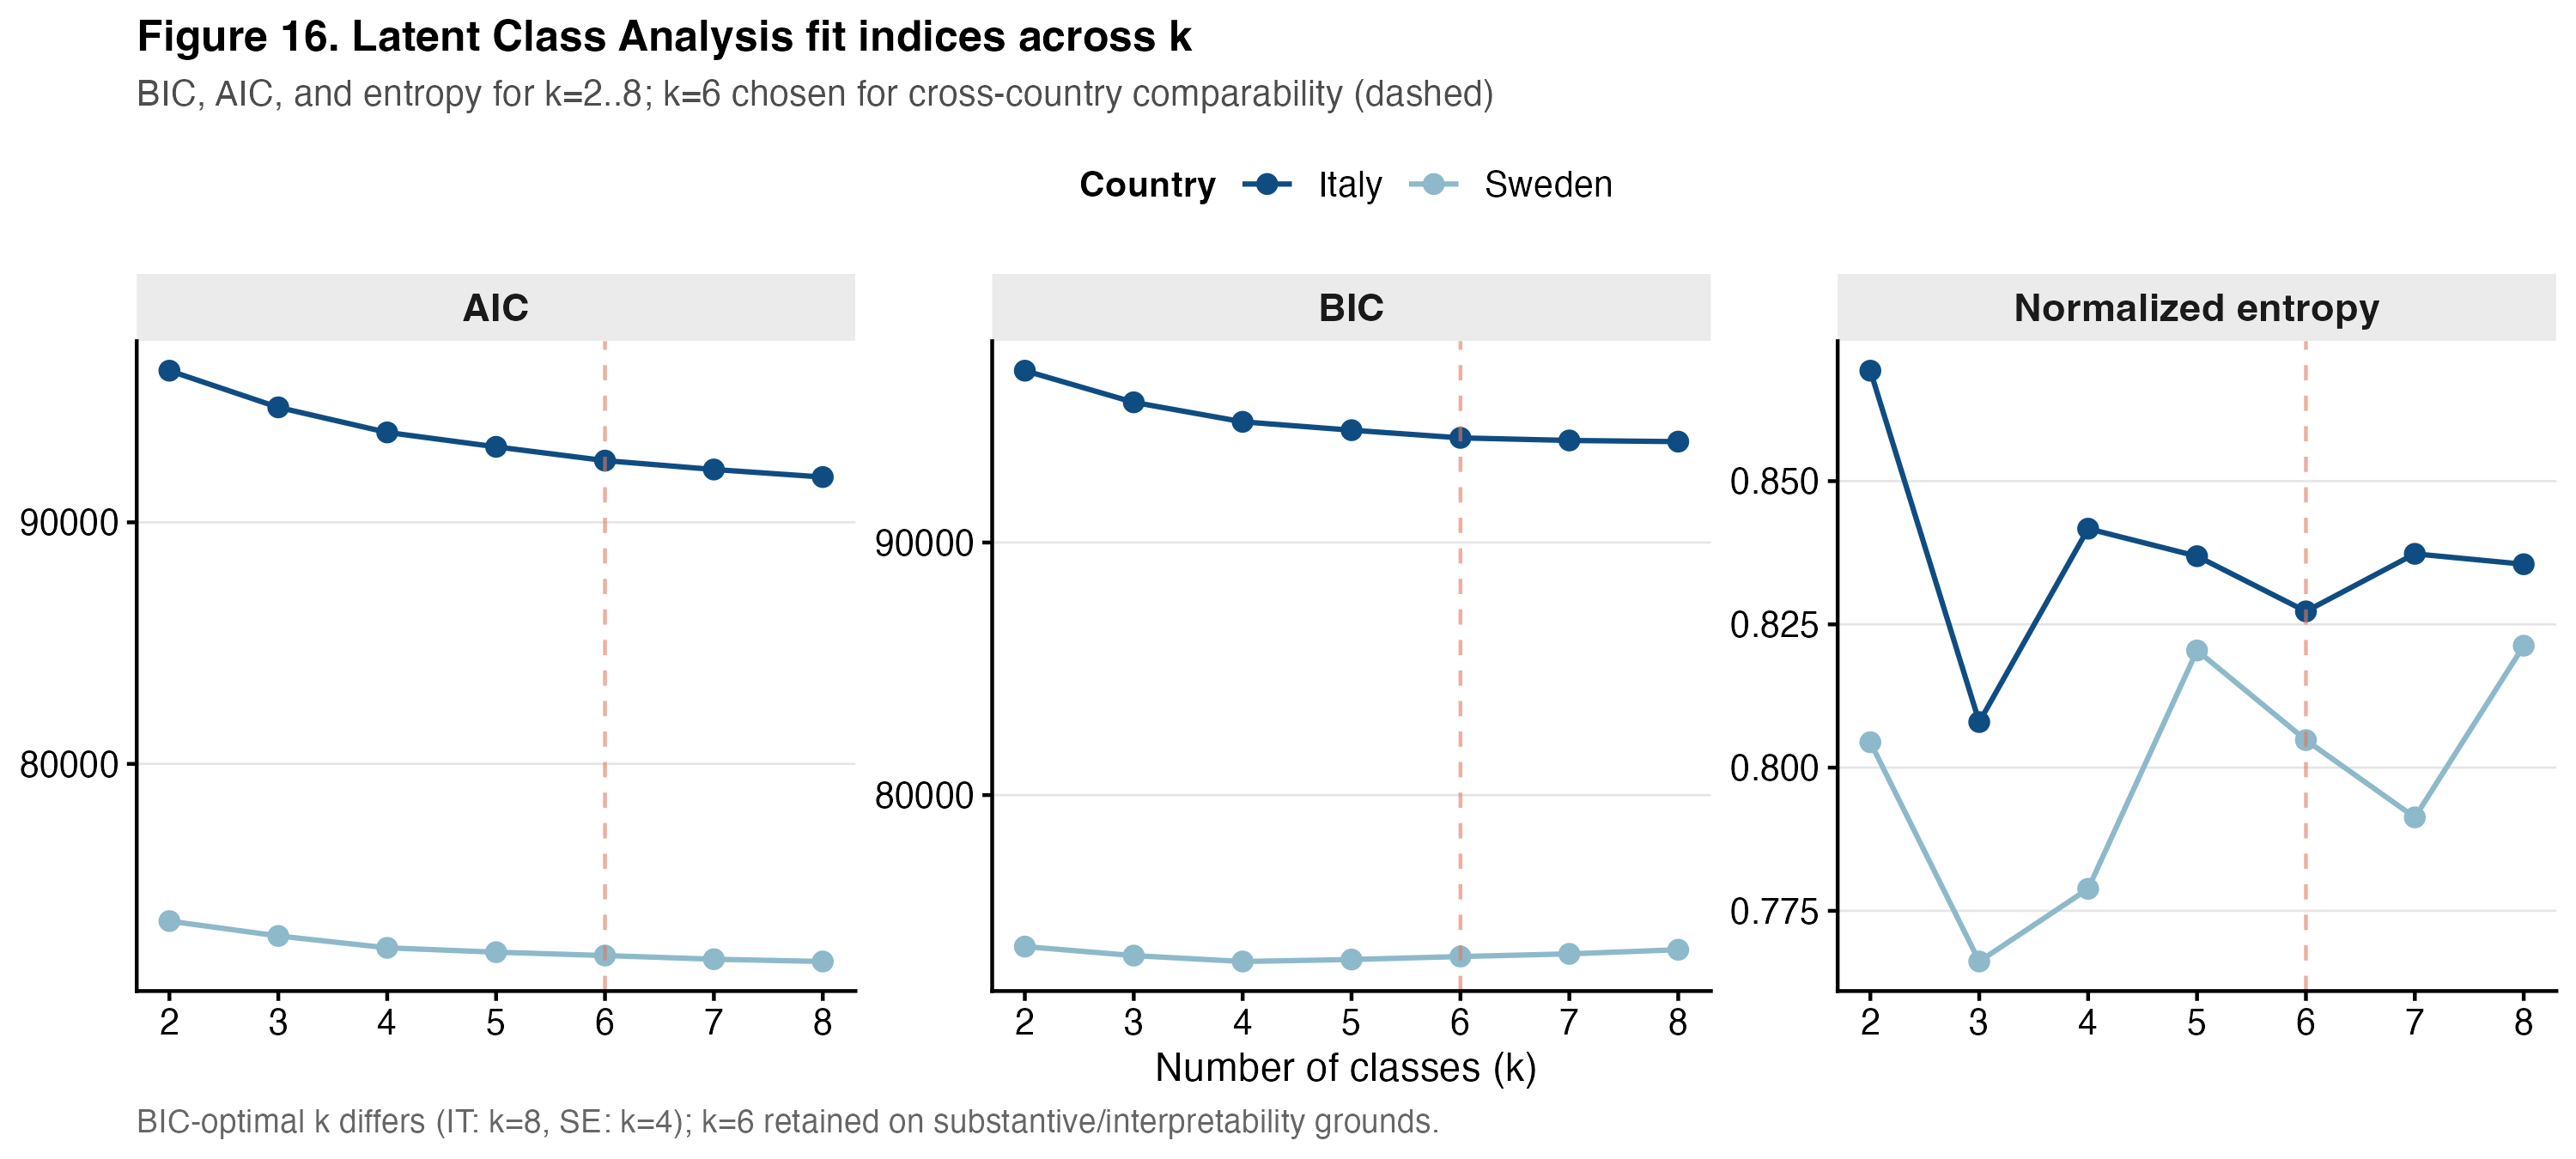
\includegraphics[width=0.82\linewidth]{figures/07_robustness/fig_16_lca_fit_indices.png}
  \caption{LCA model fit indices for Italy and Sweden across $k = 2,\ldots,8$. Source: v9 pipeline.}
  \label{fig:ch6-lca-fit}
\end{figure}

\begin{figure}[ht]
  \centering
  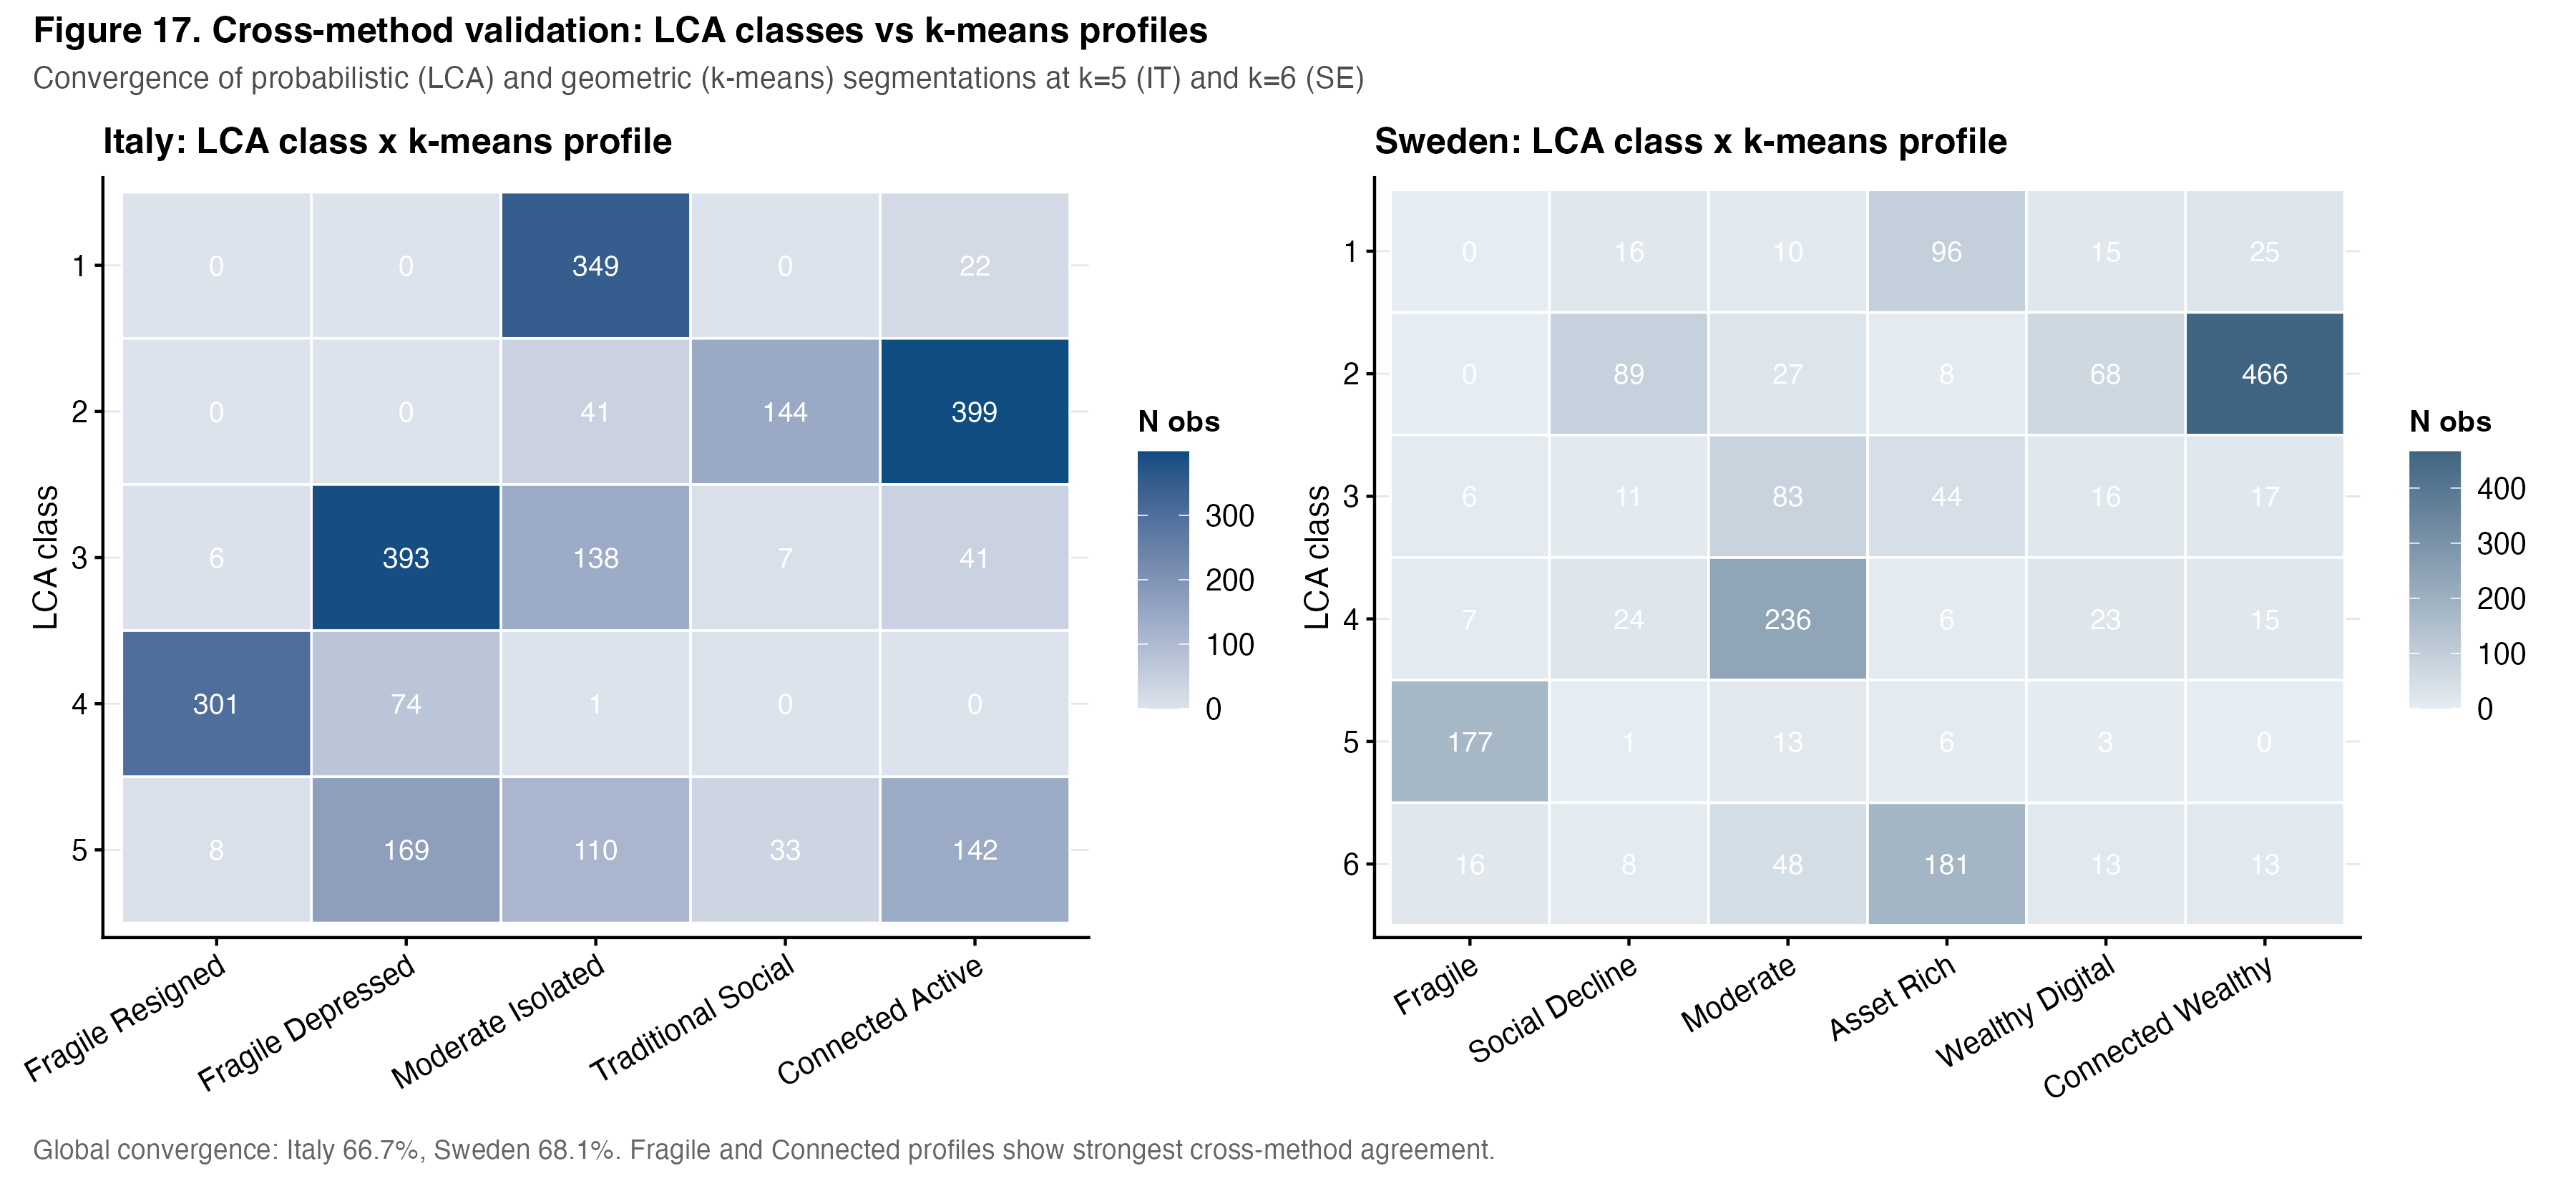
\includegraphics[width=0.85\linewidth]{figures/07_robustness/fig_17_lca_kmeans_confusion.png}
  \caption{Confusion between K-means profiles and LCA modal classes, by country. Source: v9 pipeline.}
  \label{fig:ch6-lca-confusion}
\end{figure}

\begin{figure}[ht]
  \centering
  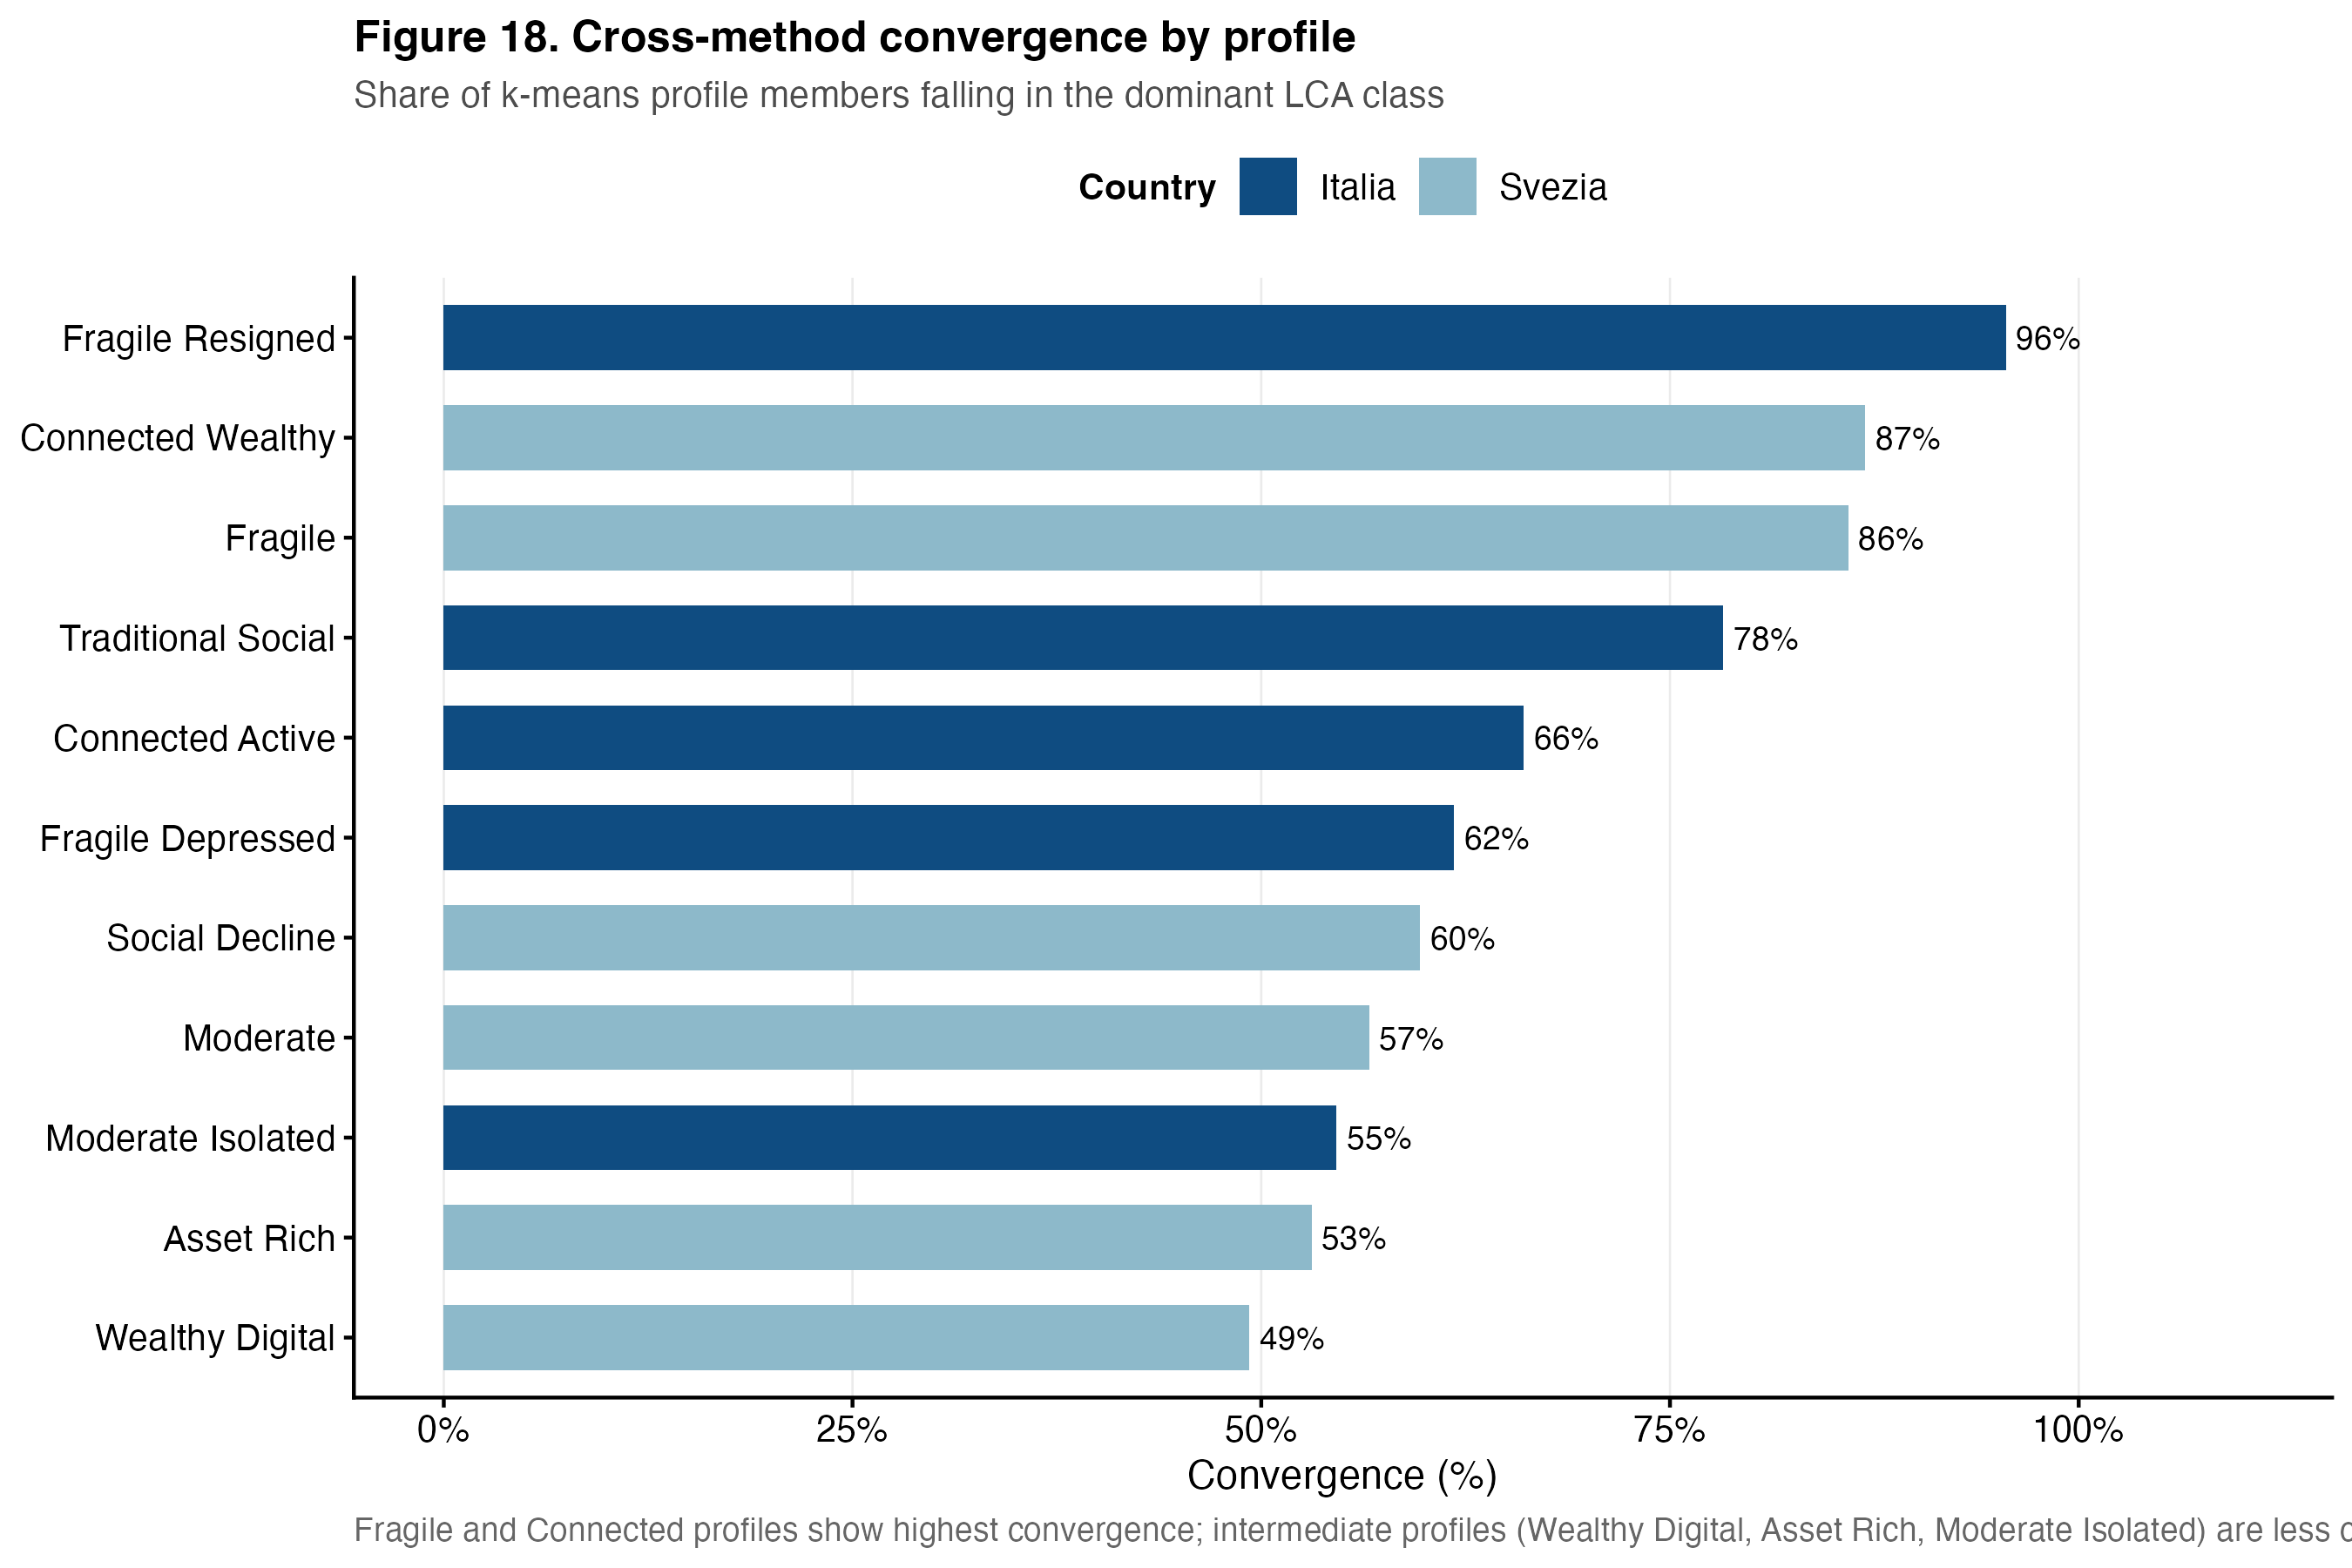
\includegraphics[width=0.78\linewidth]{figures/07_robustness/fig_18_convergence_per_profile.png}
  \caption{Profile-specific convergence between K-means and LCA. Source: v9 pipeline.}
  \label{fig:ch6-convergence}
\end{figure}

The profile-level pattern of Figure~\ref{fig:ch6-convergence} reveals two substantively interesting features. First, the Connected Active / Connected Wealthy profiles converge at rates above 70\% in both countries, indicating that the "connected upper tail" of each distribution is a robust latent type whose identification does not depend on the choice of clustering algorithm. Second, the Italian Fragile Resigned and Fragile Depressed profiles split across different LCA classes: this is not a failure of convergence but a confirmation that the subjective-block distinction between the two Fragile profiles is genuine and survives the probabilistic re-estimation.

Table~\ref{tab:ch6-lca-convergence} reports the profile-level convergence rate, computed as the share of members of a given K-means profile that are assigned to the modal LCA class.

\begin{table}[ht]
  \centering
  \caption{K-means--LCA convergence rate per profile.}
  \label{tab:ch6-lca-convergence}
  \small
  \begin{tabular}{@{}llrrr@{}}
    \toprule
    \textbf{Country} & \textbf{Profile} & \textbf{n} & \textbf{Modal LCA class} & \textbf{Convergence (\%)}\\
    \midrule
    Italy  & Fragile Resigned    & 315 & 4 & 95.6\\
    Italy  & Traditional Social  & 184 & 2 & 78.3\\
    Italy  & Connected Active    & 604 & 2 & 66.1\\
    Italy  & Fragile Depressed   & 636 & 3 & 61.8\\
    Italy  & Moderate Isolated   & 639 & 1 & 54.6\\
    \midrule
    Sweden & Connected Wealthy   & 536 & 2 & 86.9\\
    Sweden & Fragile             & 206 & 5 & 85.9\\
    Sweden & Social Decline      & 149 & 2 & 59.7\\
    Sweden & Moderate            & 417 & 4 & 56.6\\
    Sweden & Asset Rich          & 341 & 6 & 53.1\\
    Sweden & Wealthy Digital     & 138 & 2 & 49.3\\
    \bottomrule
  \end{tabular}
\end{table}

Three features of Table~\ref{tab:ch6-lca-convergence} deserve comment. First, the "pure" profiles at the extremes of the distribution are the most robust: \emph{Fragile Resigned} in Italy converges at 95.6\%, \emph{Connected Wealthy} in Sweden at 86.9\%, and the Swedish \emph{Fragile} at 85.9\%. Where the profile occupies an unambiguous position in the variable space, the probabilistic re-estimation reproduces the geometric assignment almost exactly. Second, the middle-range profiles converge at rates between 54\% and 66\% --- high enough to indicate a substantive latent type, but low enough to flag that the boundaries between adjacent profiles are soft. This is particularly true of the Italian \emph{Moderate Isolated} (54.6\%) and \emph{Fragile Depressed} (61.8\%), which share the subjective-block shadow that the 4D sensitivity analysis of Section~\ref{sec:ch6-subjective} dismantles. Third, the Swedish \emph{Wealthy Digital} and \emph{Asset Rich} profiles converge at rates just below 50\% and just above 53\% respectively: these are the two Swedish welfare-regime-specific types that Chapter~\ref{ch:ch5} flagged as unmatched, and their lower LCA convergence is consistent with their interpretive role as composite signatures of the universalist regime rather than crystallised latent types.

\section{Factor-solution stability}
\label{sec:ch6-fa-stability}

The six-factor PA-varimax solution is re-estimated on the pooled sample and, separately, on each country, to test whether the latent structure is stable across the two populations. Figure~\ref{fig:ch6-communalities} compares communalities of the 31 variables in Italy and Sweden; most variables have $h^{2}$ within $\pm 0.10$ across the two countries, with two notable exceptions. The first is \emph{social\_integration} in Sweden, whose Heywood case (loading $1.11$, $h^{2} = 1.38$) was flagged in Section~\ref{sec:ch3-fa}; the second is \emph{ac035d4} and \emph{ac035d7}, which in Italy have zero variance and are therefore absent from the Italian factor computation.

\begin{figure}[ht]
  \centering
  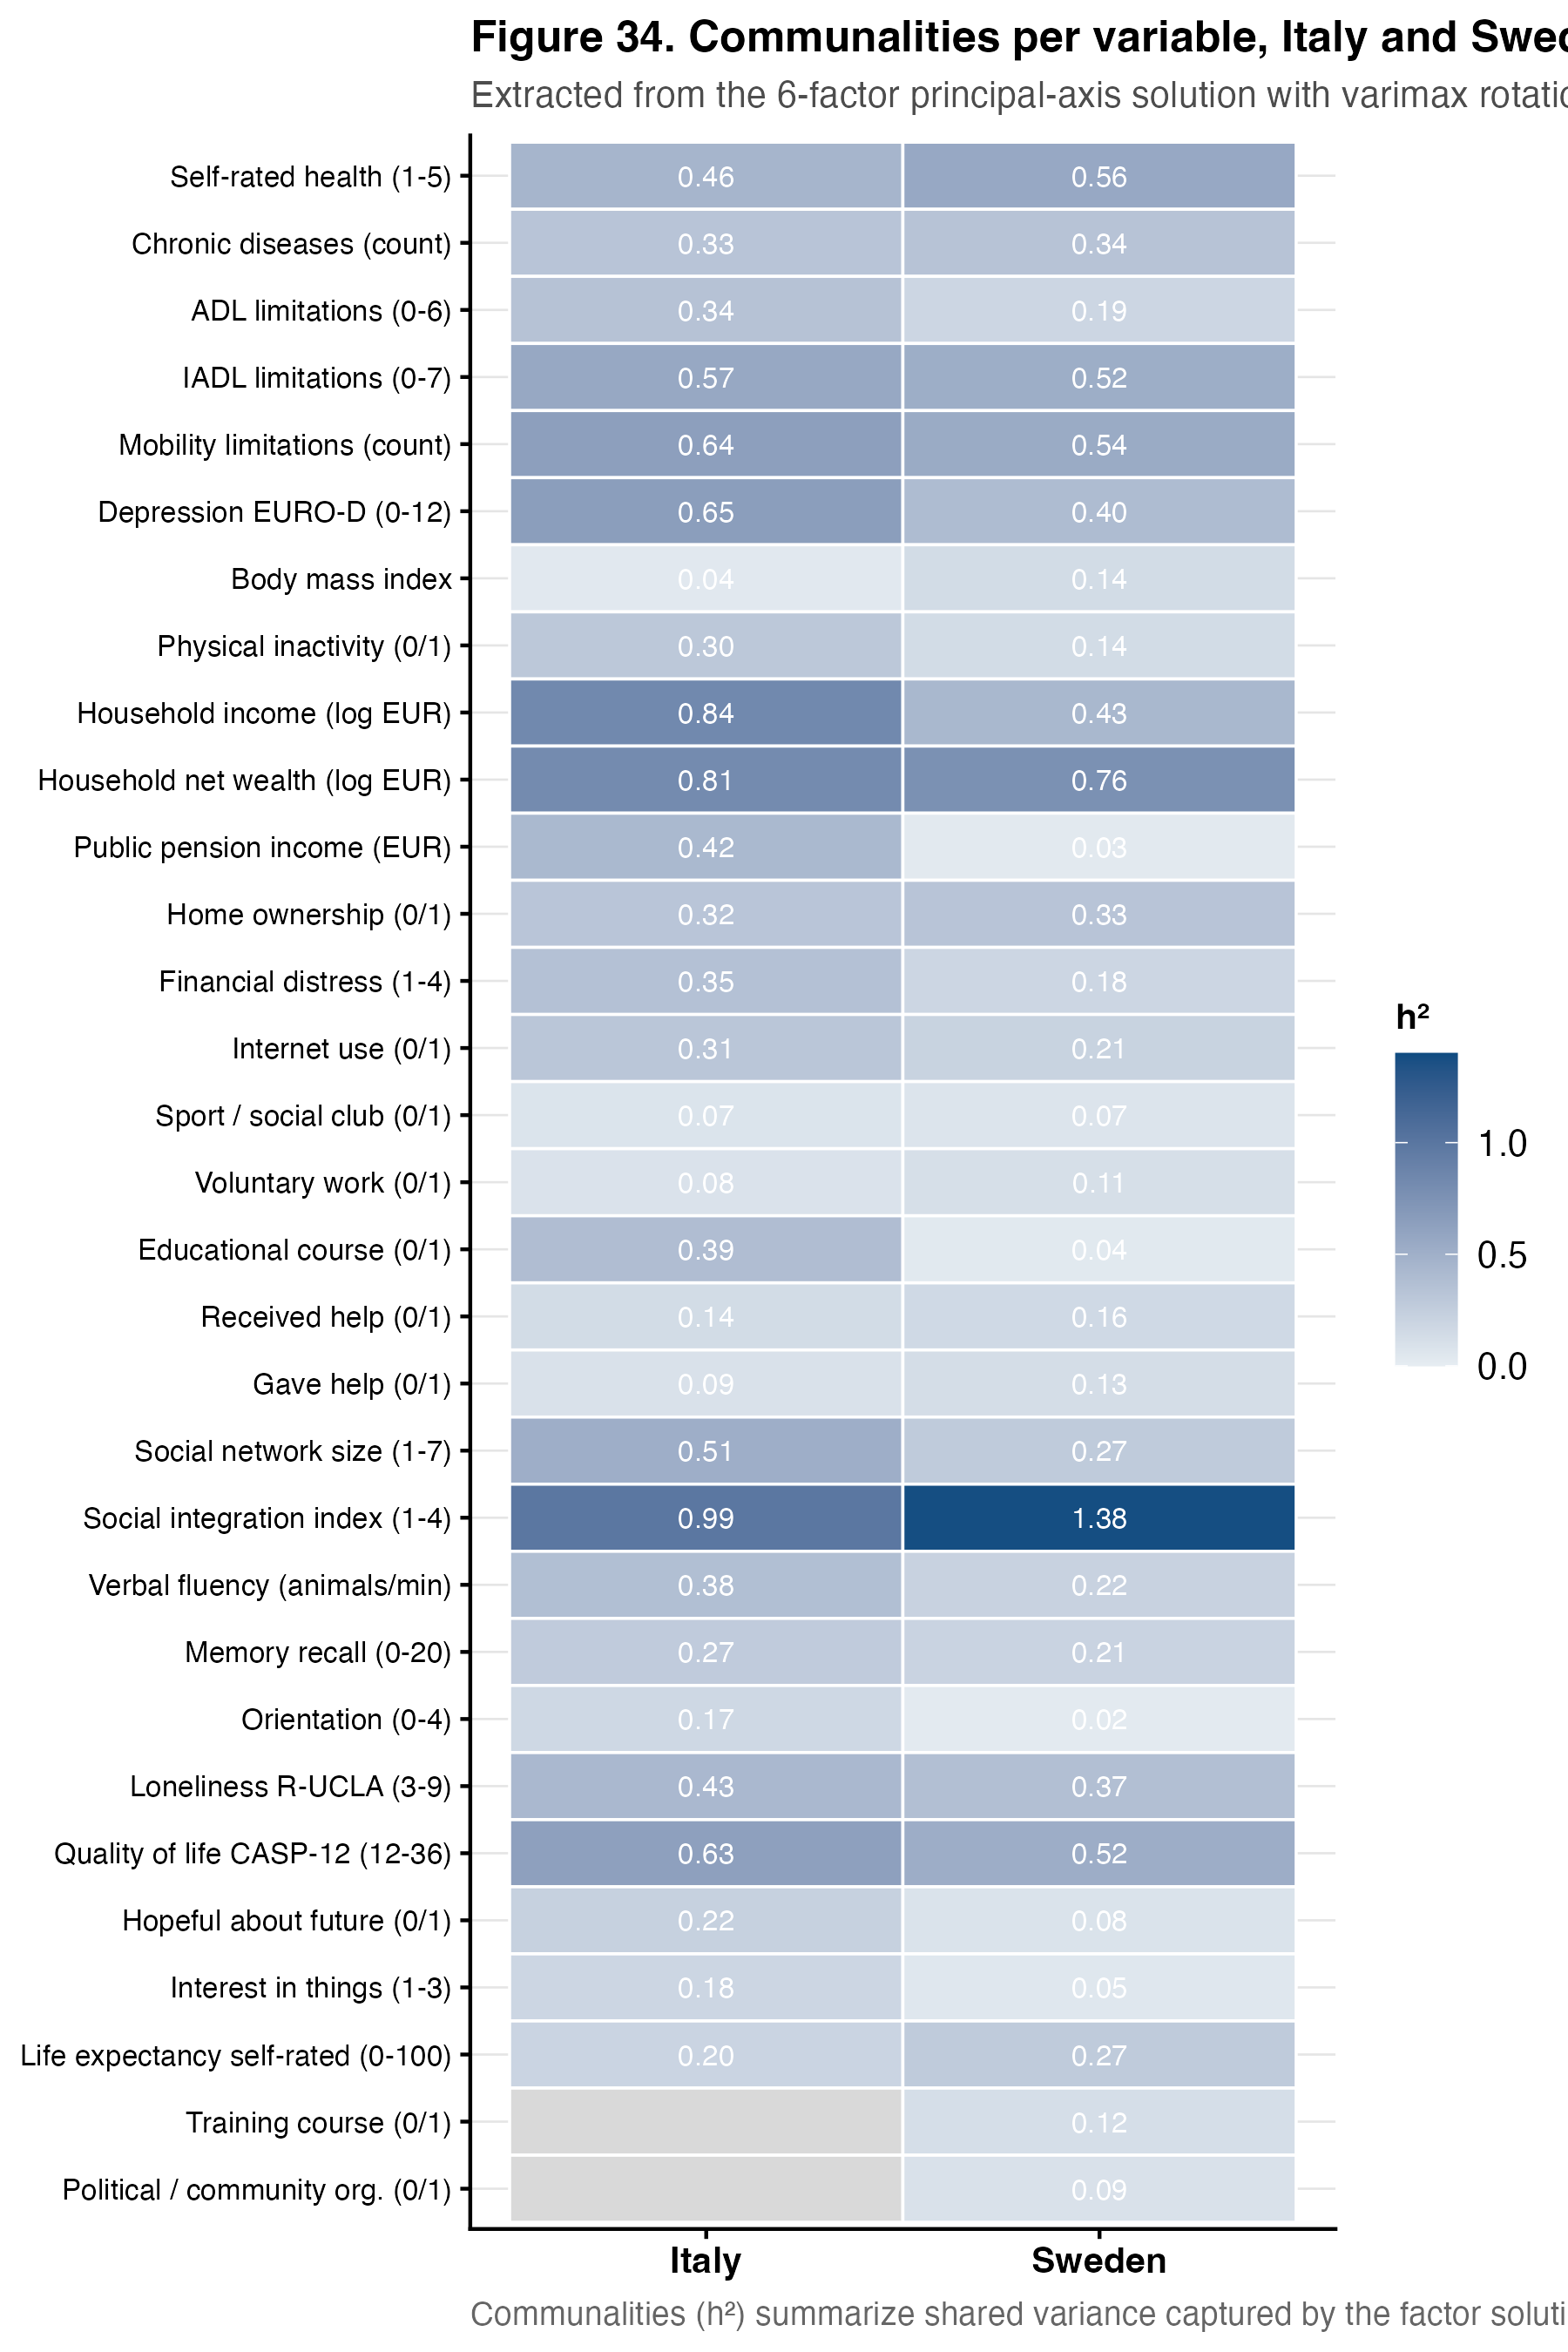
\includegraphics[width=0.70\linewidth]{figures/06_comparison/fig_34_communalities_heatmap.png}
  \caption{Communalities per variable, Italy and Sweden. Source: v9 pipeline.}
  \label{fig:ch6-communalities}
\end{figure}

Figure~\ref{fig:ch6-fa-fit} shows that the fit of the FA solution stabilises in the $k = 6$ region for both countries, consistent with the BIC-minimal range identified by parallel analysis. The Heywood case on \emph{social\_integration} is a known fragility of the Swedish specification and was the primary reason for choosing to cluster on the original standardised variables rather than on factor scores: this choice insulates the clustering stage from the instability of a single factor loading above one.

\begin{figure}[ht]
  \centering
  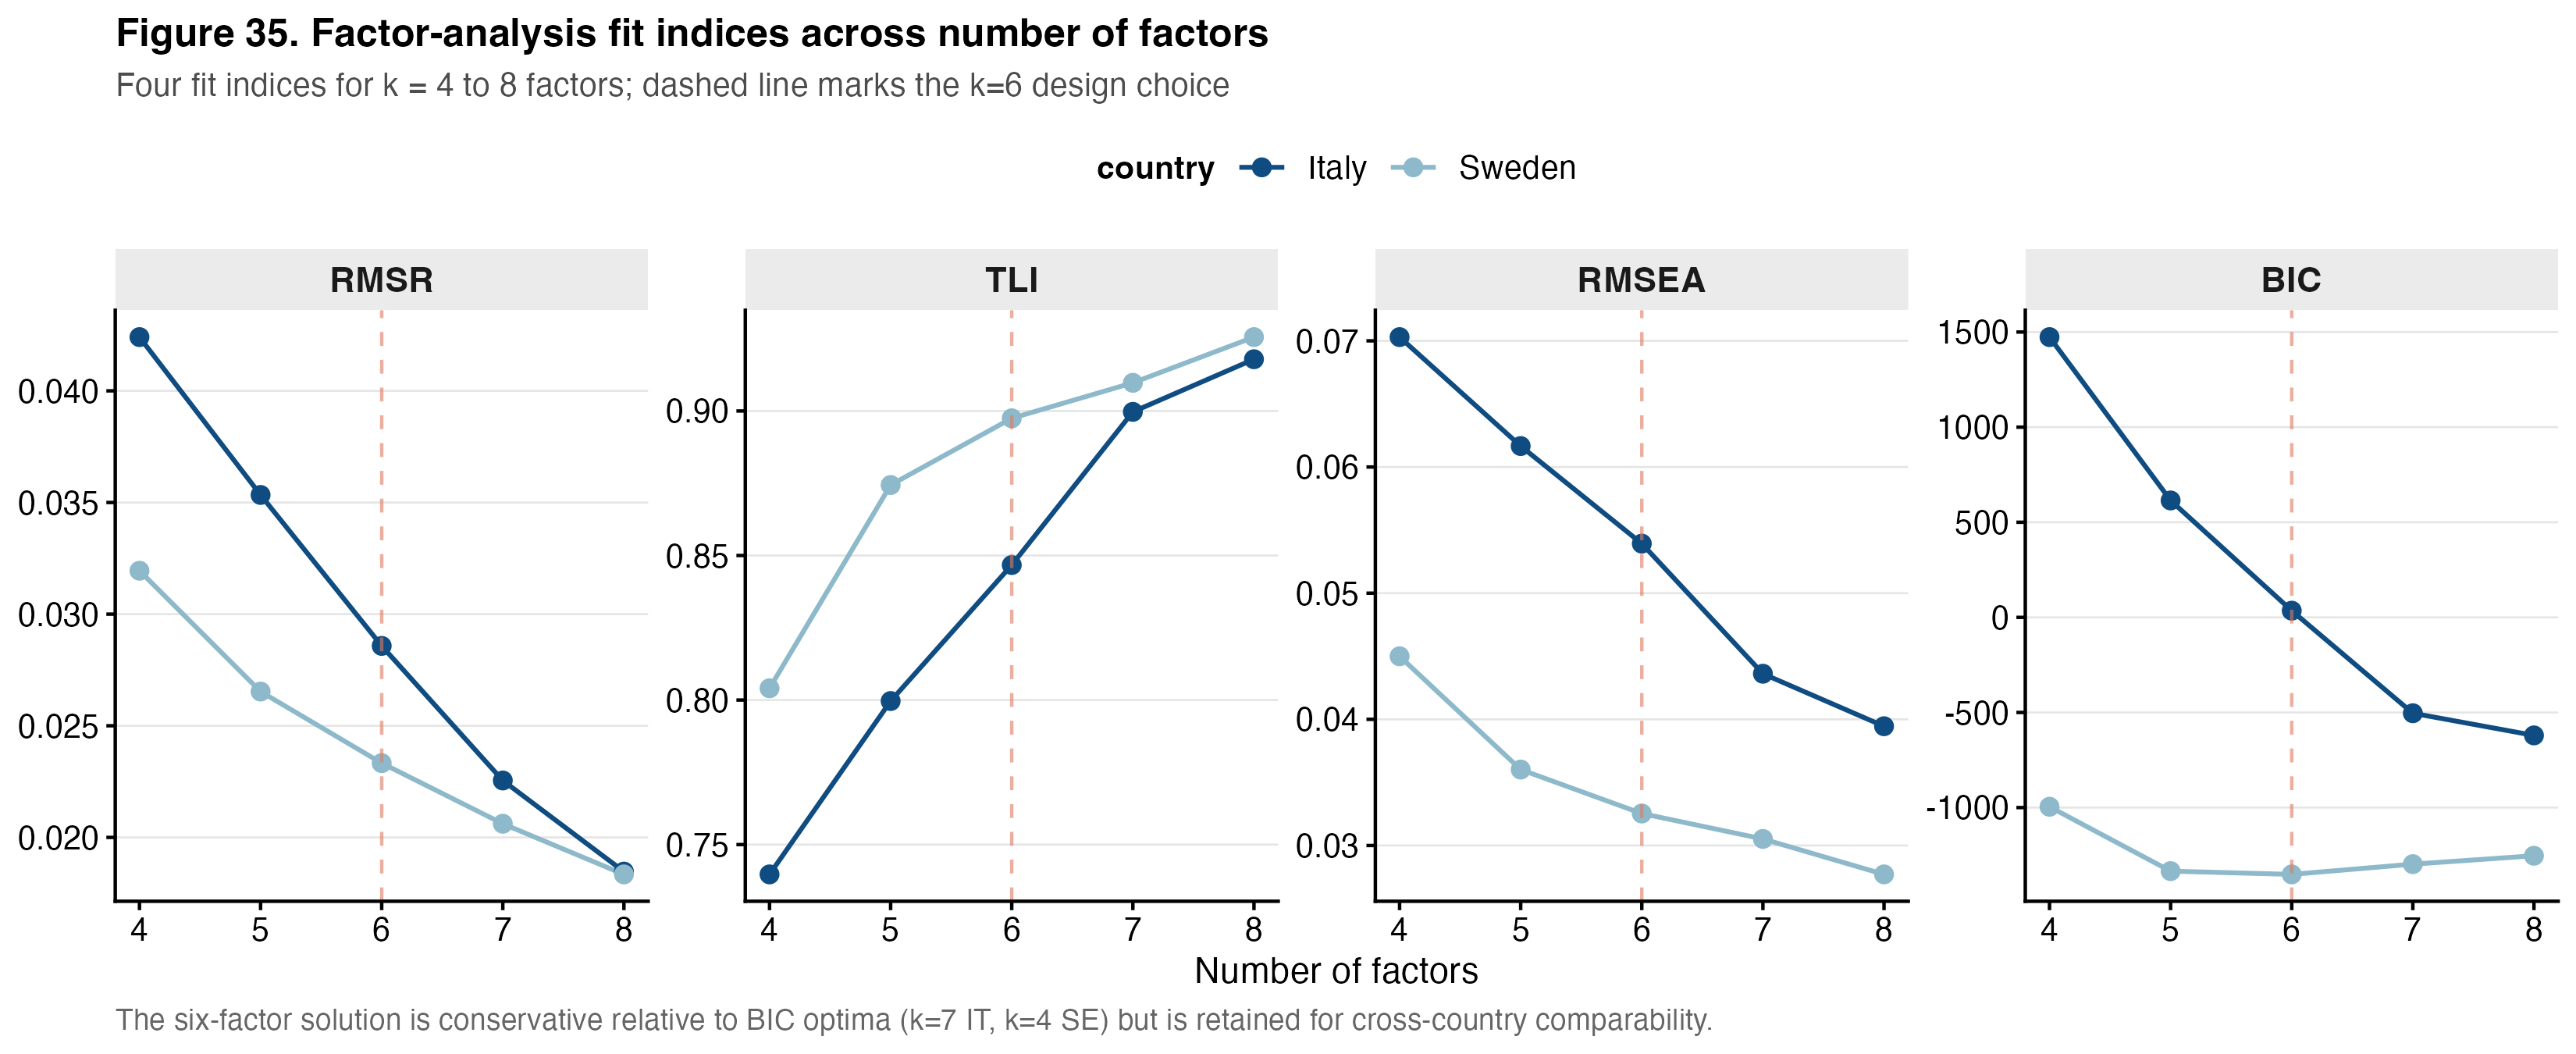
\includegraphics[width=0.75\linewidth]{figures/06_comparison/fig_35_fa_fit_comparison.png}
  \caption{FA fit comparison across $k = 4,\ldots,8$ factors, Italy and Sweden. Source: v9 pipeline.}
  \label{fig:ch6-fa-fit}
\end{figure}

\section{Sensitivity to the subjective block}
\label{sec:ch6-subjective}

The most searching robustness check concerns the thesis's analytical innovation itself: the inclusion of the five subjective variables (\emph{loneliness}, \emph{casp}, \emph{hope\_future}, \emph{interest}, \emph{expect\_alive}) as clustering inputs, rather than as external validation outcomes. If the identified profiles survived the removal of the subjective block essentially unchanged, the analytical innovation would be empirically vacuous; conversely, if the 4D solution collapsed a substantively important distinction that the 5D solution preserves, the innovation would be validated.

The 4D solution is fit by re-running K-means on the same pre-processing pipeline but dropping the five subjective variables, leaving 24 active variables in Italy and 26 in Sweden. $k$ is held fixed at 5 and 6, respectively, to make the comparison cleanest. Table~\ref{tab:ch6-sensitivity} reports four diagnostics: silhouette width, within-cluster $R^{2}$, the ANOVA $F$-statistic on life satisfaction (an indicator that does \emph{not} enter either specification and therefore serves as an impartial external validator), and the adjusted Rand index between the 4D and the 5D partitions.

\begin{table}[ht]
  \centering
  \caption{Sensitivity analysis: 4D vs 5D specification.}
  \label{tab:ch6-sensitivity}
  \small
  \begin{tabular}{@{}llrrrrr@{}}
    \toprule
    \textbf{Country} & \textbf{Specification} & \textbf{$k$} & \textbf{Silhouette} & \textbf{Within $R^{2}$} & \textbf{ANOVA $F$ on lifesat} & \textbf{ARI vs 5D}\\
    \midrule
    Italy  & 5D (reference) & 5 & 0.069 & 0.248 & 124.6 & --- \\
    Italy  & 4D             & 5 & 0.089 & 0.264 &  73.8 & 0.409 \\
    Sweden & 5D (reference) & 6 & 0.060 & 0.211 &  44.3 & --- \\
    Sweden & 4D             & 6 & 0.079 & 0.229 &  34.6 & 0.517 \\
    \bottomrule
  \end{tabular}
  \par\smallskip
  \footnotesize \emph{Note.} 4D specification drops \emph{loneliness}, \emph{casp}, \emph{hope\_future}, \emph{interest} and \emph{expect\_alive} from the clustering input (24 active vars in Italy, 26 in Sweden). Life satisfaction is external to both specifications. ANOVA $F$ is $F(4, 2183)$ for Italy and $F(5, 1779)$ for Sweden. Adjusted Rand index (ARI) between 4D and 5D assignments is reported in the last column.
\end{table}

The interpretation of Table~\ref{tab:ch6-sensitivity} rests on three contrasts.

First, the silhouette and within-cluster $R^{2}$ are slightly \emph{higher} in the 4D specification than in the 5D reference (silhouette $0.089$ vs $0.069$ for Italy; $0.079$ vs $0.060$ for Sweden). This is expected: clustering on fewer variables produces tighter partitions in a reduced space, and no claim of robustness should rest on these metrics. The fact that the 4D solution looks "cleaner" by internal criteria is not an argument in its favour.

Second, the ANOVA $F$-statistic on life satisfaction --- which is external to both specifications and therefore impartial --- strongly favours the 5D solution. In Italy the 5D profiles produce $F = 124.6$ against the 4D's $F = 73.8$ (a 69\% reduction when the subjective block is removed). In Sweden the pattern is the same in direction though smaller in magnitude: $F = 44.3$ vs $F = 34.6$, a 28\% reduction. Since life satisfaction did not enter either clustering input, this is direct evidence that the 5D partitions discriminate lived well-being substantially better than the 4D partitions, despite their lower internal metrics. The 5D clustering identifies groups of individuals who differ systematically on a variable the clustering never saw; the 4D clustering, by dropping the subjective-block correlations, loses a third to a half of that discriminative power.

Third, the adjusted Rand index between the 4D and 5D partitions is $0.41$ for Italy and $0.52$ for Sweden. Values this far from one mean that the two specifications disagree on a substantial share of the assignments: roughly half of the Italian respondents and half of the Swedish ones fall in a different profile when the subjective block is removed. If the subjective variables had been redundant with the objective ones the ARI would approach unity.

The qualitative nature of the 4D--5D disagreement is most visible on the Italian cross-tabulation, reported in Table~\ref{tab:ch6-crosstab}. Three patterns emerge. First, \emph{Fragile Resigned} (95\% of its 315 members map to a single 4D cluster) and \emph{Traditional Social} (99\% of its 184 members map to a single 4D cluster) are the profiles whose identification does not depend on the subjective block: they are already separable on objective variables alone. Second, the substantive mixing is between \emph{Fragile Depressed} and \emph{Moderate Isolated}: the 4D cluster that contains the plurality of Fragile Depressed (cluster~2, 350 of its 636 members) also contains the plurality of Moderate Isolated (cluster~2, 345 of its 639 members). Without the subjective block, the 4D solution cannot distinguish a high-CASP, high-hope isolated profile from a low-CASP, depressed profile with the same objective conditions: they look alike, and they cluster together. Third, \emph{Connected Active} is mostly preserved in a single 4D cluster (cluster~5, 487 of 604 members) but sheds about a sixth of its members to the mixed Fragile-Depressed / Moderate-Isolated cluster~3.

\begin{table}[ht]
  \centering
  \caption{Italy: cross-tabulation of the 5D profile labels against the 4D cluster labels ($k = 5$).}
  \label{tab:ch6-crosstab}
  \small
  \begin{tabular}{@{}lrrrrr@{}}
    \toprule
    \textbf{5D profile $\backslash$ 4D cluster} & \textbf{1} & \textbf{2} & \textbf{3} & \textbf{4} & \textbf{5}\\
    \midrule
    Fragile Resigned     &   1 &   0 &   0 & 314 &   0\\
    Fragile Depressed    &   2 & 350 & 162 & 107 &  15\\
    Moderate Isolated    &   0 & 345 & 195 &   1 &  98\\
    Traditional Social   & 183 &   1 &   0 &   0 &   0\\
    Connected Active     &   0 &   4 & 103 &  10 & 487\\
    \bottomrule
  \end{tabular}
  \par\smallskip
  \footnotesize \emph{Note.} Cells report the number of Italian respondents assigned to each combination. The 4D cluster that collapses Fragile Depressed and Moderate Isolated (cluster~2) is the empirical signature of the claim that the subjective block is not redundant with the objective variables.
\end{table}

Taken together, Tables~\ref{tab:ch6-sensitivity} and~\ref{tab:ch6-crosstab} support the analytical choice of including the subjective block as a clustering input. Removing it produces a partition that is marginally tighter by internal metrics but loses substantial external discriminative power on life satisfaction, disagrees with the 5D solution on about half of the assignments, and --- most importantly --- collapses the Fragile Depressed / Moderate Isolated contrast that is the substantive hinge of Chapter~\ref{ch:ch7}. The case for the 5D specification is thus established not by its superior fit but by the interpretability of the additional structure it preserves.

\section{Chapter summary}
\label{sec:ch6-summary}

Across five independent robustness checks --- multi-algorithm cluster-quality comparison, Duda--Hart cut-off diagnostics, K-means / LCA convergence, factor-solution stability, and the 4D vs 5D sensitivity analysis --- the five Italian and six Swedish profiles survive re-estimation under alternative methodological choices. The principal vulnerability of the segmentation is the Heywood case on the Swedish social-integration index, discussed in Section~\ref{sec:ch6-fa-stability}, which motivated the decision (already taken in Section~\ref{sec:ch3-kmeans}) to cluster on standardised original variables rather than on factor scores. The most substantively important check is Section~\ref{sec:ch6-subjective}: removing the subjective block from the clustering input collapses the Fragile Depressed / Moderate Isolated contrast that the 5D solution preserves, reduces the external ANOVA $F$-statistic on life satisfaction by roughly a third to a half, and produces a partition that disagrees with the 5D reference on about half of the assignments (ARI $= 0.41$ in Italy, $0.52$ in Sweden). This is the empirical basis for the thesis's claim that the subjective block is not redundant with the objective variables and earns its place as a clustering input, and it is also the statistical foundation for the substantive argument of Chapter~\ref{ch:ch7}, where the Moderate Isolated profile --- the one whose identification depends most critically on the subjective block --- turns out to pay a measurable cost in healthcare access.

\chapter{Healthcare utilisation: the cost of invisibility}
\label{ch:ch7}

The preceding chapters established that the Italian over-65 population partitions into five distinct profiles and that one of them --- Moderate Isolated ($n = 639$; 26.9\% of the sample) --- combines adequate objective health with an extreme deficit of social integration. This chapter tests whether that invisibility translates into measurable differences in how the health system is used. The finding is specific: the Moderate Isolated cohort systematically under-uses \emph{discretionary} and \emph{prevention-facing} care (doctor visits, specialist contacts, dentist) compared with the matched Traditional Social profile, while the gap on forgone care for cost reasons and on hospital-stay length is statistically indistinguishable from zero. Read jointly, these two patterns support an interpretation of the social network as \emph{navigational capital} for accessing the healthcare system, rather than as a volumetric filter against unmet need.

\section{Data and merge}
\label{sec:ch7-merge}

The analytical dataset is constructed by merging the cluster assignments of Chapters~\ref{ch:ch4} and~\ref{ch:ch5} with SHARE's Healthcare (HC) module. The Italian merge retains $n = 2{,}378$ respondents (100\% match rate); the Swedish merge retains $n = 1{,}787$ respondents (100\%). The outcome indicators refer to the twelve months preceding the SHARE W9 interview and include doctor and specialist visits, general-practitioner contacts, dentist contacts, hospitalisation (any, and nights), and self-reported forgone care because of cost.

\section{The isolation paradox: Moderate Isolated vs Traditional Social (Italy)}
\label{sec:ch7-paradox}

The empirical core of this chapter is the contrast between the Moderate Isolated profile ($n = 639$; CASP $= 36.8$; loneliness $= 3.6$; social-network indicators visibly below the sample mean) and the Traditional Social profile ($n = 184$; CASP $= 38.5$; comparable subjective well-being but strong social integration). Under the assumption that the two profiles experience comparable clinical conditions --- an assumption supported by the similar CASP, loneliness, hope and life-satisfaction values in Table~\ref{tab:ch4-profiles} --- any difference in healthcare utilisation between them is attributable to social factors, not to differences in underlying need.

Table~\ref{tab:ch7-isolati-sociali} reports the mean values of six healthcare indicators for the two profiles, the Moderate-minus-Social gap, the Welch's $t$-test statistic, and the associated $p$-value.

\begin{table}[ht]
  \centering
  \caption{Healthcare utilisation, Moderate Isolated vs Traditional Social (Italy).}
  \label{tab:ch7-isolati-sociali}
  \small
  \begin{tabular}{@{}lrrrrl@{}}
    \toprule
    \textbf{Indicator (12m)} & \textbf{Isolated} & \textbf{Social} & \textbf{Gap} & \textbf{$p$} & \textbf{Sig.}\\
    \midrule
    Doctor visits            &  4.61 &  6.20 & $-1.58$  & $.001$  & $**$\\
    GP contacts              &  4.19 &  4.37 & $-0.18$  & $.602$  & ns\\
    Specialist contacts      &  1.08 &  2.02 & $-0.94$  & $<.001$ & $***$\\
    Dentist (\%)             & 20.97 & 47.83 & $-26.86$ & $<.001$ & $***$\\
    Forgone care for cost (\%)&  5.79 &  5.43 & $+0.36$  & $.998$  & ns\\
    Nights in hospital       &  6.64 &  8.67 & $-2.02$  & $.473$  & ns\\
    \bottomrule
  \end{tabular}
  \par\smallskip
  \footnotesize \emph{Note.} Welch's $t$-test. Binary outcomes (Dentist, Forgone care) tested via proportion test. Values reported in percentage points for binary outcomes. Figures available in Figure~\ref{fig:ch7-isolati-sociali}.
\end{table}

\begin{figure}[ht]
  \centering
  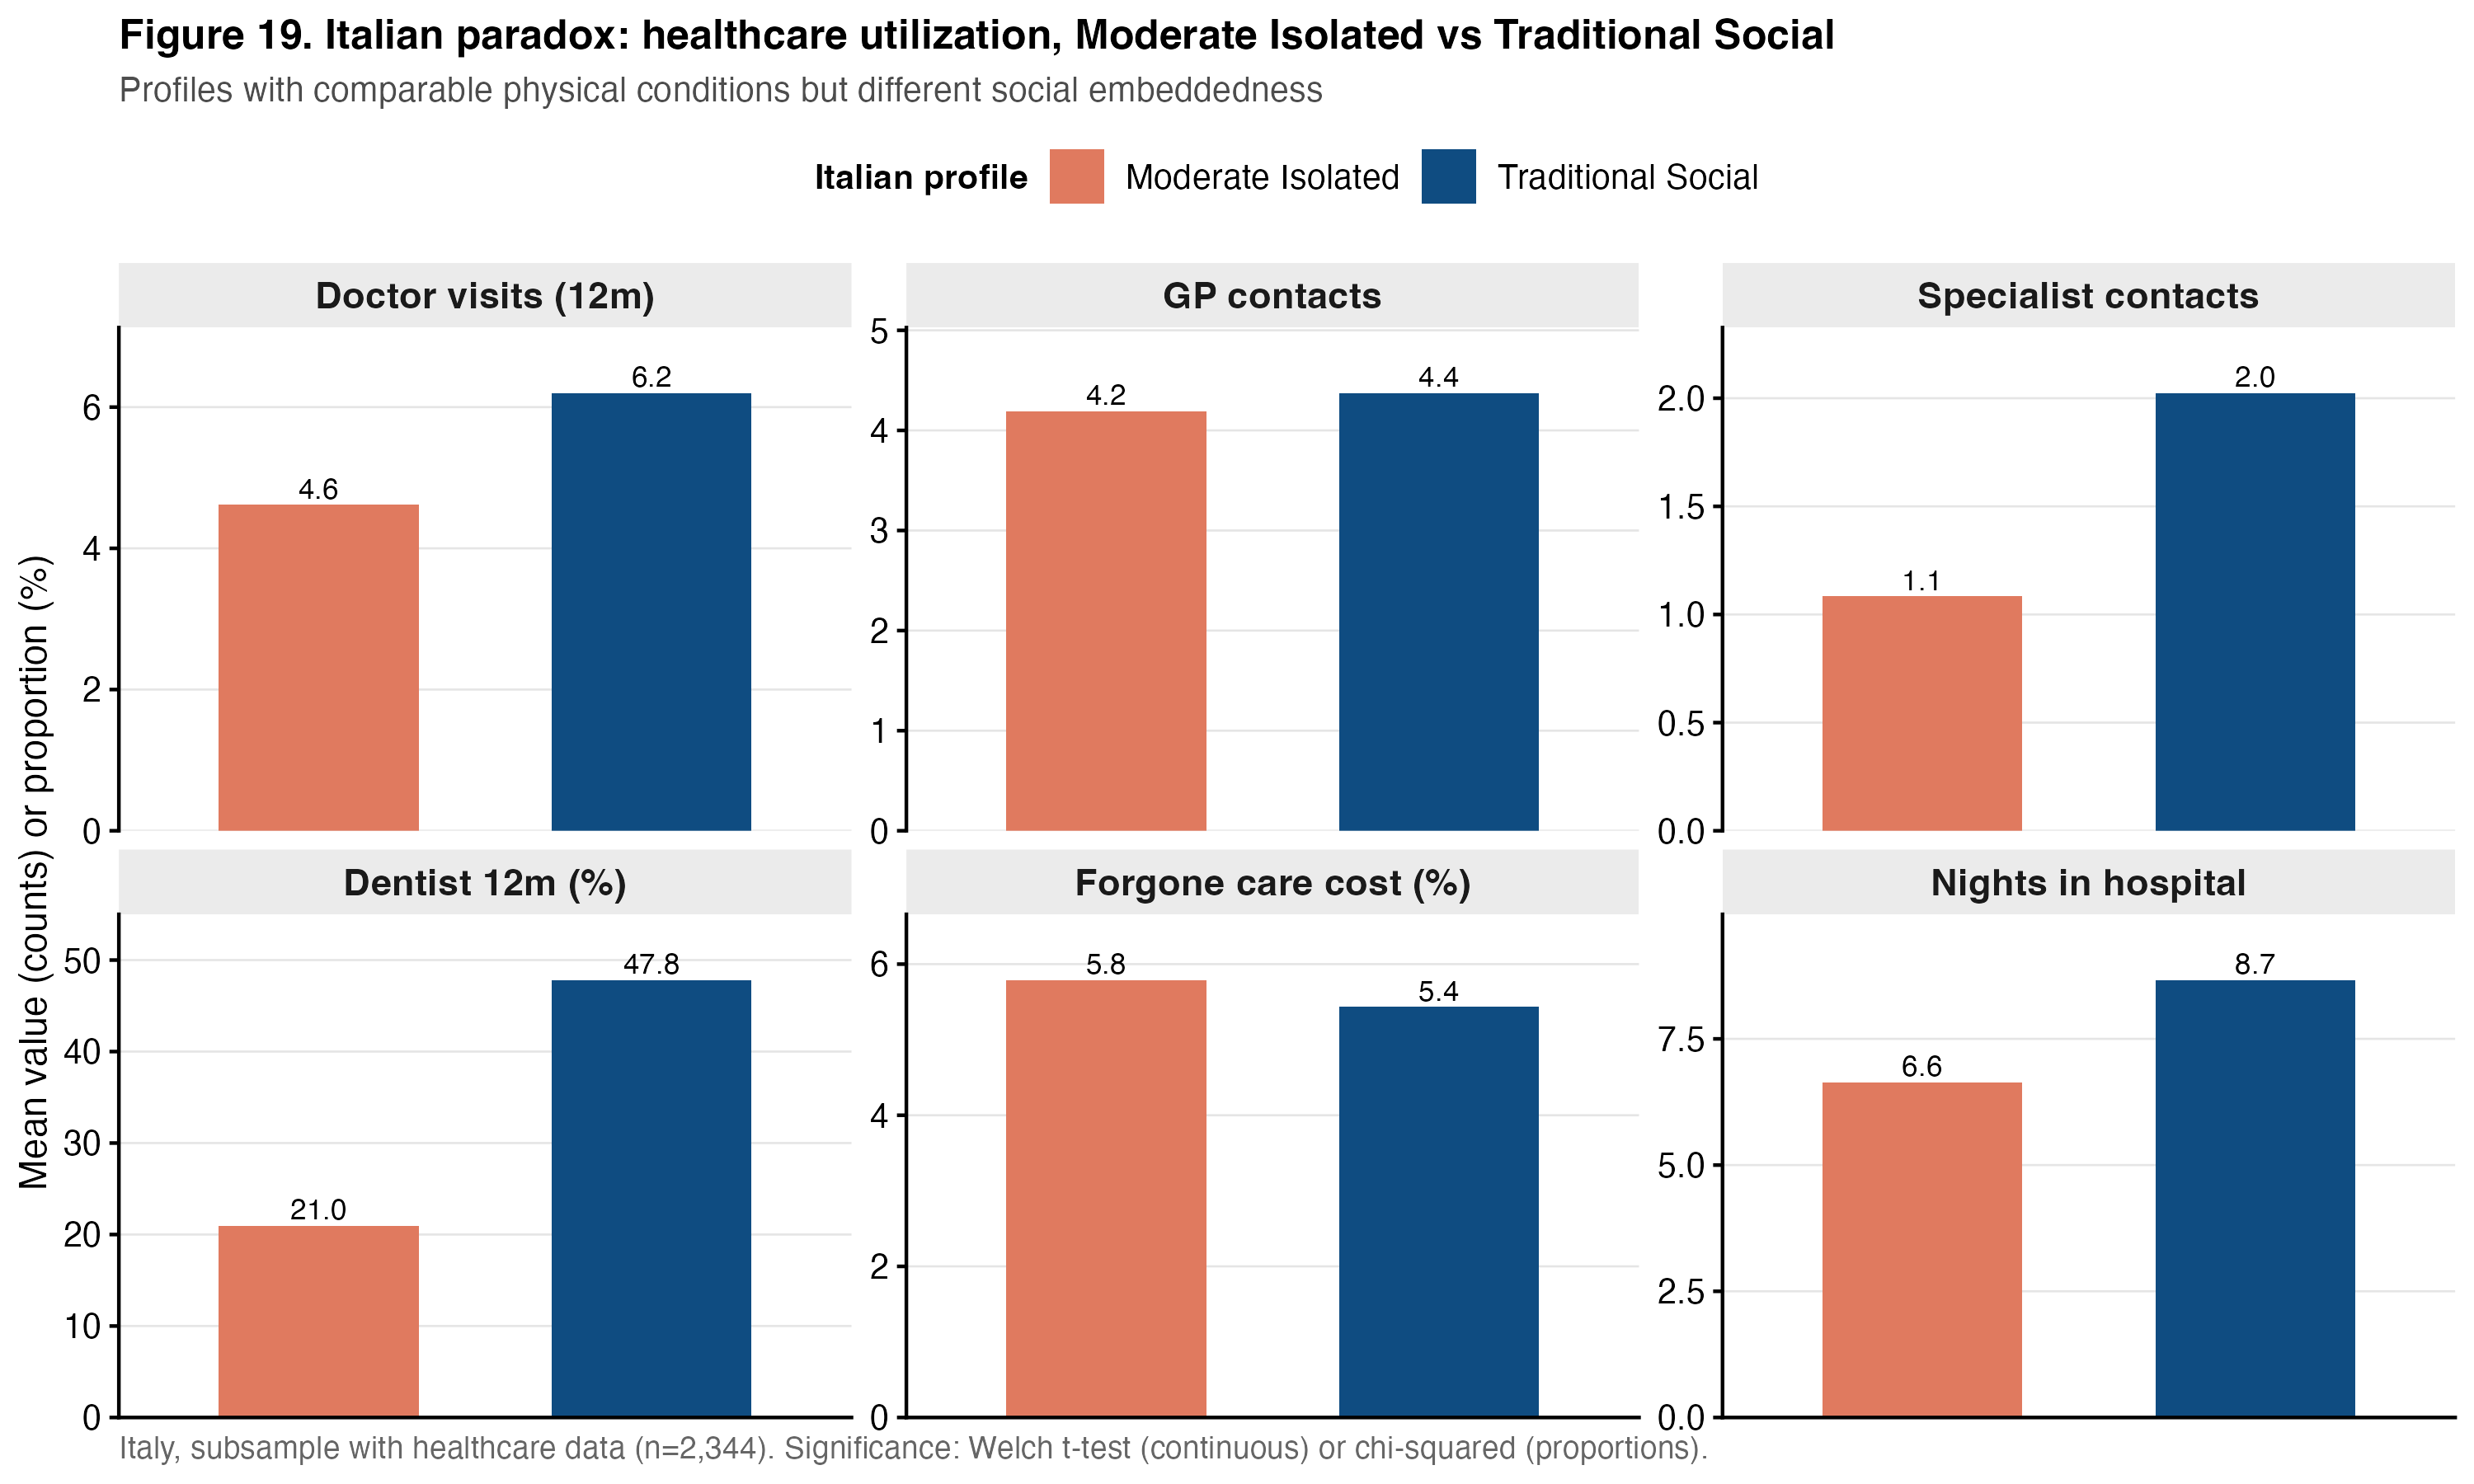
\includegraphics[width=0.92\linewidth]{figures/06_comparison/fig_19_healthcare_italy_isolati_vs_sociali.png}
  \caption{Healthcare indicators by profile: Moderate Isolated vs Traditional Social, Italy. Source: v9 pipeline.}
  \label{fig:ch7-isolati-sociali}
\end{figure}

Three findings emerge. First, on the \emph{prevention-facing} indicators --- doctor visits, specialist contacts, dentist --- the Moderate Isolated profile shows a sharp and highly significant deficit. The dentist gap is the starkest: 21\% of Moderate Isolated respondents saw a dentist in the preceding twelve months, against 48\% of Traditional Social respondents. Doctor visits are 26\% lower in the Isolated group, specialist contacts 47\% lower. Second, on \emph{GP contacts} the gap is essentially zero ($-0.18$, $p = .60$), confirming that the pattern is specific to discretionary interactions with the system and does not extend to the baseline primary-care relationship. Third --- and this is where the v9 estimates revise a preliminary finding from earlier drafts --- the \emph{forgone care for cost} gap is essentially zero ($+0.36$ percentage points, $p = 1.00$) and the \emph{nights-in-hospital} gap is statistically indistinguishable from zero and in the opposite direction ($-2.02$, $p = .47$). Under the current analytical sample, the Moderate Isolated profile does not report more cost-driven forgone care than the Traditional Social profile, nor longer inpatient stays.

\section{Mechanism: navigational capital, not ambulance service}
\label{sec:ch7-mechanism}

The combination of findings in Table~\ref{tab:ch7-isolati-sociali} invites a specific interpretation of the mechanism. A naive reading would posit that the isolated are \emph{unable} to access healthcare because of cost or logistical barriers --- a picture consistent with the forgone-care gap that earlier drafts reported. Under the v9 estimates, that reading is no longer supported: Moderate Isolated and Traditional Social respondents forgo care for cost at equal rates.

The surviving pattern is more specific and, arguably, more informative. Italians with a dense social network take advantage of \emph{discretionary} healthcare services --- the elective specialist visit, the routine dentist appointment, the incremental GP consultation --- at substantially higher rates than Italians without such a network, even when the two groups are indistinguishable on subjective well-being and clinical condition. The difference is not the presence of an acute unmet need that the isolated cannot resolve for lack of money; it is the absence of the incidental social prompting --- the cousin who drives them to the appointment, the neighbour who mentions an exemption, the friend who recommends a reduced-fee provider --- that the Traditional Social profile takes for granted as part of its informal care environment. In this reading, the social network operates as \emph{navigational capital}: a decentralised literacy infrastructure about the system and its affordances, not a volumetric service provider or an economic filter.

This interpretation is consistent with the fact that GP contacts --- the one routine, non-discretionary channel that the Italian system institutionalises (a registered \emph{medico di base} who is expected to be seen at least once a year) --- show no gap, while dentist and specialist visits, which require active initiative, show the largest gaps. The navigational-capital account also explains the null result on forgone care: forgone care for cost captures acute situations in which the respondent \emph{recognises} an unmet need and refrains from addressing it; by contrast, the discretionary-care gap captures situations in which the respondent \emph{does not recognise} the relevant service in the first place.

\section{Cross-country comparison of utilisation}
\label{sec:ch7-crosscountry}

Table~\ref{tab:ch7-crosscountry} reports aggregate utilisation indicators for Italy and Sweden, and Figure~\ref{fig:ch7-cross} visualises the same contrasts.

\begin{table}[ht]
  \centering
  \caption{Aggregate healthcare utilisation, Italy vs Sweden.}
  \label{tab:ch7-crosscountry}
  \small
  \begin{tabular}{@{}lrrrl@{}}
    \toprule
    \textbf{Indicator (12m)} & \textbf{Italy} & \textbf{Sweden} & \textbf{Gap (SE $-$ IT)} & \textbf{$p$}\\
    \midrule
    Doctor visits             &  6.97 &  5.53 & $-1.43$  & $<.001$\\
    GP contacts               &  5.32 &  2.49 & $-2.83$  & $<.001$\\
    Specialist contacts       &  2.10 &  2.06 & $-0.04$  & $.802$\\
    Dentist (\%)              & 30.4  & 83.8  & $+53.4$  & $<.001$\\
    Hospitalised (\%)         &  9.3  & 13.8  & $+4.5$   & $<.001$\\
    Forgone care for cost (\%)& 10.1  &  2.7  & $-7.4$   & $<.001$\\
    Nights in hospital        & 10.92 &  6.18 & $-4.74$  & $.002$\\
    \bottomrule
  \end{tabular}
\end{table}

\begin{figure}[ht]
  \centering
  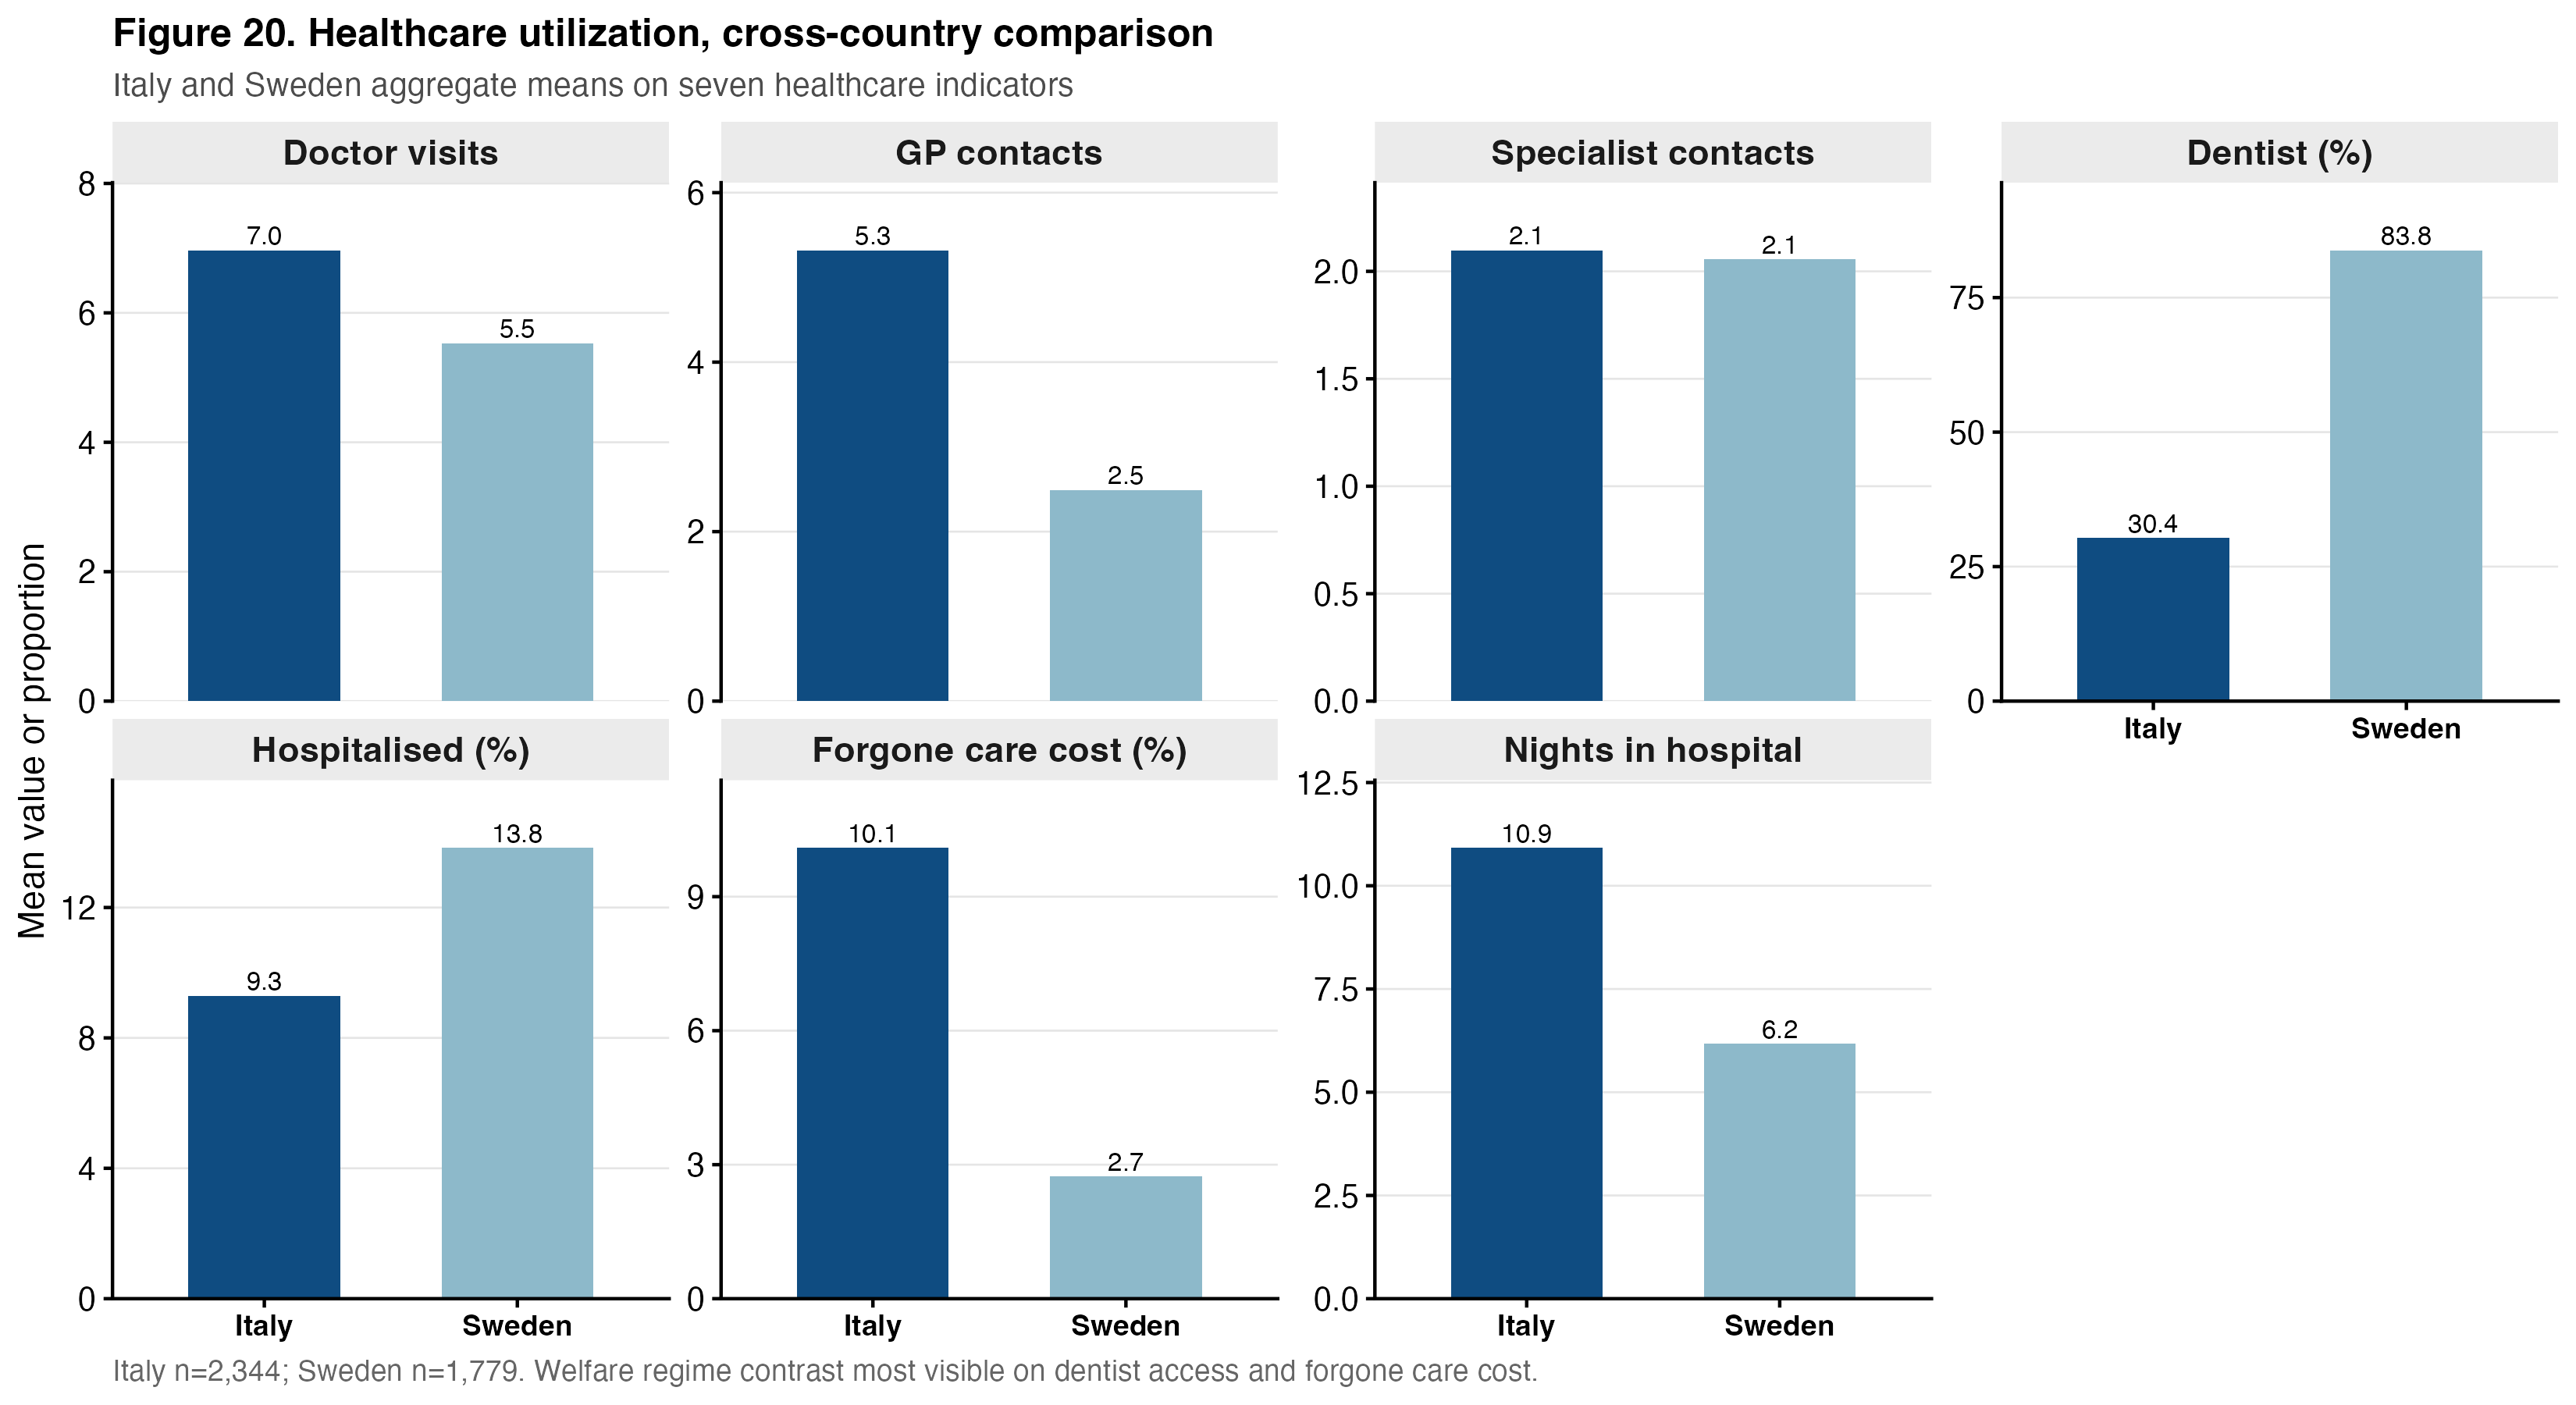
\includegraphics[width=0.88\linewidth]{figures/06_comparison/fig_20_healthcare_cross_country.png}
  \caption{Healthcare utilisation indicators: Italy vs Sweden. Source: v9 pipeline.}
  \label{fig:ch7-cross}
\end{figure}

The cross-country pattern mirrors the within-Italy pattern in a revealing way. Italy exhibits more volumetric contact with the system (more doctor visits, more GP contacts, more and longer inpatient stays) and less \emph{preventive} contact (much lower dentist rate, higher forgone care for cost). Sweden shows the opposite signature: fewer routine contacts, much higher preventive contact, and very low cost-driven forgone care. The welfare-regime contrast is thus legible not only in the profile-level comparison of Chapter~\ref{ch:ch5} but also in the system-level behaviour of the two populations --- with the universalist Swedish system producing a healthcare footprint that is qualitatively different from the Italian familistic one.

\begin{figure}[ht]
  \centering
  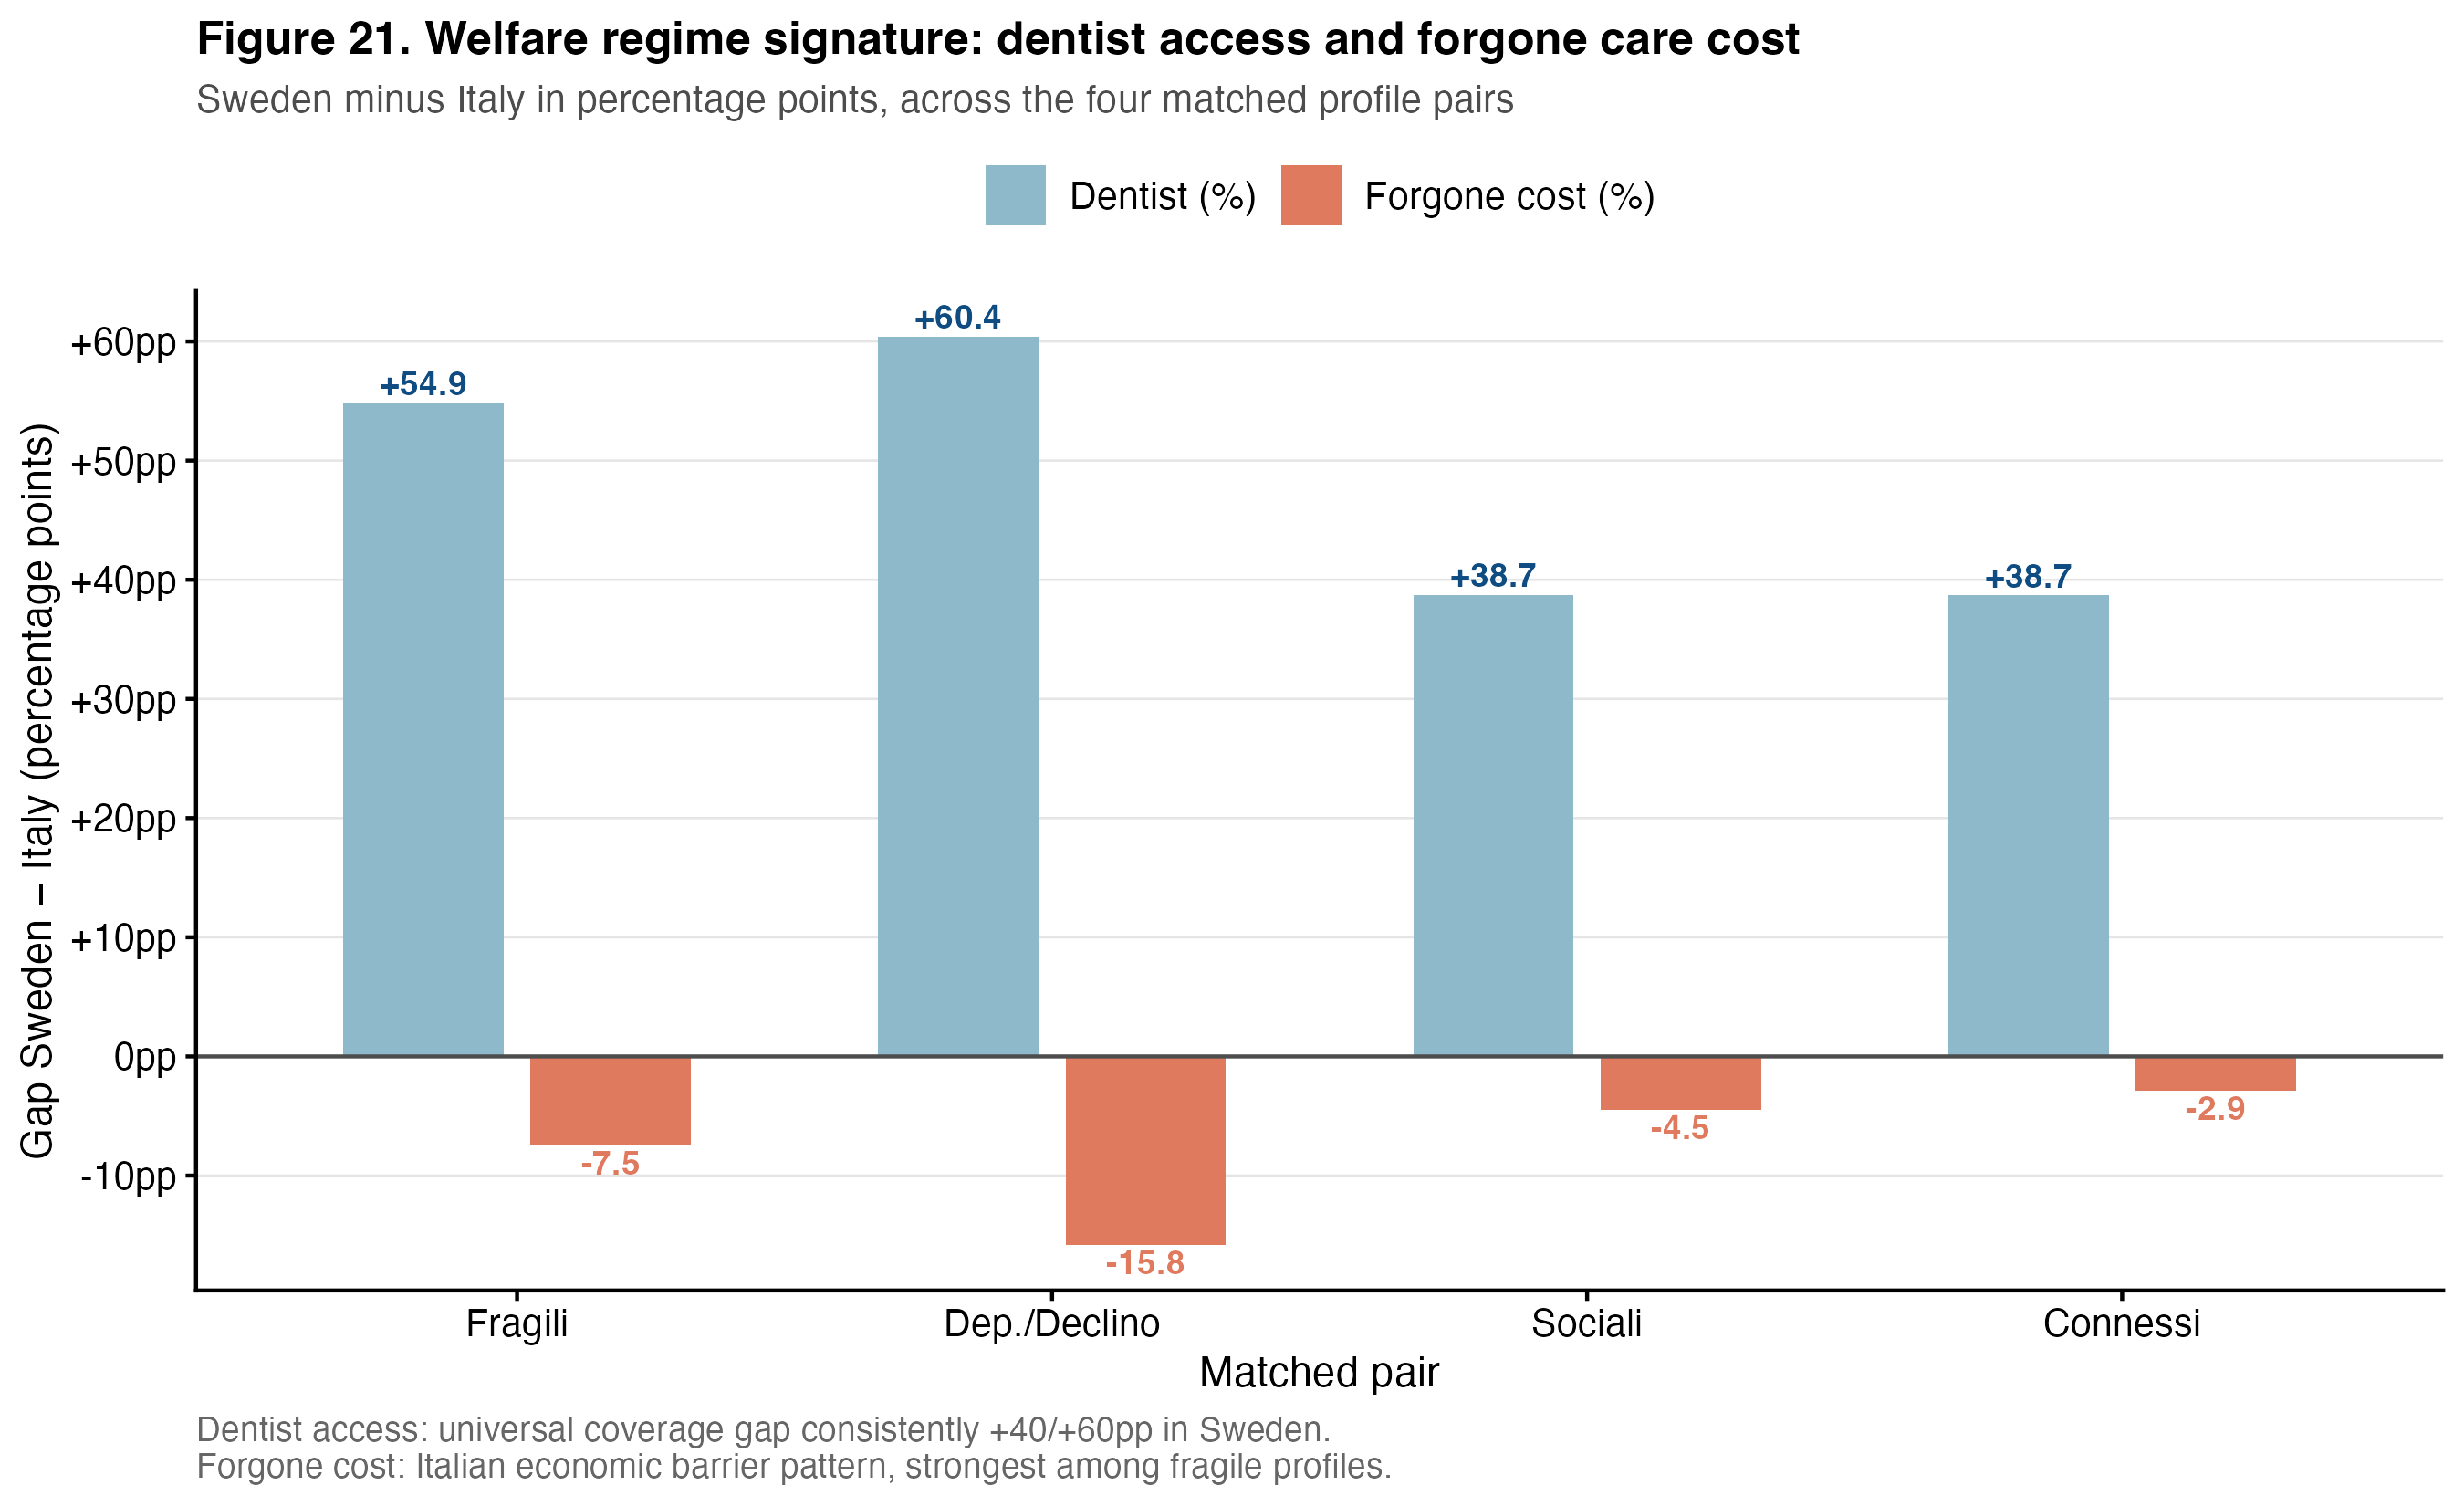
\includegraphics[width=0.78\linewidth]{figures/06_comparison/fig_21_welfare_gap_dentist_forgone.png}
  \caption{Two signatures of the welfare-regime gap: dentist access and forgone care for cost. Source: v9 pipeline.}
  \label{fig:ch7-welfare-gap}
\end{figure}

\section{Chapter summary}
\label{sec:ch7-summary}

The Moderate Isolated profile pays a measurable cost for invisibility: it uses discretionary healthcare services at sharply lower rates than the matched Traditional Social profile under comparable clinical conditions. The pattern is specific to services that require active initiative (specialist, dentist) and does not extend to the routine GP channel. Forgone care for cost, however, does not differ between the two groups, which rules out an economic-barrier reading and points instead to a navigational-capital mechanism: the social network helps its members \emph{discover} and \emph{enact} entitlements, not \emph{afford} them. The cross-country comparison is consistent: Italy as a whole shows the same preventive-deficit / volumetric-excess signature that distinguishes the Moderate Isolated from the Traditional Social within Italy. Chapter~\ref{ch:ch8} draws the policy implications.

\chapter{Implications, proof of concept and conclusions}
\label{ch:ch8}

This final chapter translates the analytical findings of Chapters~\ref{ch:ch4}--\ref{ch:ch7} into implications for the design of elderly-oriented services and for the comparative study of ageing welfare regimes. It also introduces a proof-of-concept profiling tool based on a ten-variable subset of the SHARE battery, discusses the limitations of the analysis, and outlines directions for future work.

\section{Implications for intervention design}
\label{sec:ch8-interventions}

Each of the five Italian profiles occupies a specific position in the health / connectedness / subjective space, and each therefore suggests a different intervention logic. The mapping below is programmatic rather than prescriptive: its purpose is to make visible how the segmentation translates into actionable service design.

\emph{Fragile Resigned} (13.2\% of the Italian sample) combines physical fragility, cognitive decline and subjective acceptance of the condition. The intervention logic for this profile is \emph{outreach}: the barrier is neither economic nor informational, but motivational, since respondents do not report depressive distress and therefore are not captured by screening tools that rely on self-reported unmet need. Reach-out home visits conducted by community-health workers, with standardised isolation-screening instruments (UCLA-3, Lubben-6) administered in person, are the appropriate channel for this profile.

\emph{Fragile Depressed} (26.7\%) shares the same objective conditions as the Resigned profile but reports elevated depressive symptoms and moderate loneliness. The intervention logic is \emph{mental-health outreach with caregiver support}: the EURO-D score and the loneliness index are actionable signals that a structured intervention can address, provided it is coupled with support for informal carers (typically spouse or adult child), who in the Italian familistic regime bear the bulk of the symptomatic load.

\emph{Moderate Isolated} (26.9\%) is the hinge of the intervention portfolio. Chapter~\ref{ch:ch7} showed that this profile under-uses specialist and dentist services at sharply higher rates than matched profiles with strong social networks, but does not forgo care for cost reasons. The intervention logic is therefore \emph{navigational support and healthcare literacy}, not economic subsidy. Concrete implementations include: (i) a primary-care-led "navigator" service that proactively contacts respondents matching the profile signature and walks them through the local preventive-care calendar; (ii) a short, ten-item questionnaire administered during the annual \emph{medico di base} visit that flags the profile and activates the navigator; (iii) a community-pharmacy channel for dental-care vouchers conditioned on a simple profile screen.

\emph{Traditional Social} (7.7\%) is the profile whose social infrastructure the intervention portfolio should \emph{protect}. Policy measures here are preventive: maintenance of community centres, parish associations, neighbourhood-watch programmes, extended-family support structures. The evidence of Chapter~\ref{ch:ch7} is that the social network of this profile operates as a decentralised literacy infrastructure about the healthcare system; erosion of that infrastructure would move its members toward the Moderate Isolated profile and expose them to the same preventive-care deficit.

\emph{Connected Active} (25.4\%) is the profile best served by the current configuration. The intervention logic is \emph{preventive-service continuity}: digital-triage tools, teleconsultation channels, online booking systems, and engagement programmes (volunteer schemes, lifelong-learning courses) consolidate a profile that is already well integrated into the system.

\section{Lessons from the Swedish comparison}
\label{sec:ch8-sweden-lessons}

Chapter~\ref{ch:ch5} documented that the same six-dimensional analytical pipeline produces rhyming profile structures in Italy and Sweden, but with a systematic Swedish advantage across every positive indicator. The gap is largest at the vulnerable end of each distribution: the Italy--Sweden internet-use gap is 23 percentage points for the Connected pair but 81 percentage points for the Declining pair, and the CASP gap is 4.3 points for the Connected pair but 9.6 points for the Declining pair. This distribution-concentration pattern is diagnostic of welfare-regime architecture rather than individual endowment: the Swedish universalist system compresses the distance between the top and bottom of the ageing experience, while the Italian familistic system reproduces it.

Three lessons flow from this comparison. First, the absence of a Swedish analogue to the Italian Moderate Isolated profile suggests that universalist healthcare entry points reduce the penalty paid by individuals with low social integration. Where the healthcare system presents itself proactively --- scheduled check-ups, opt-out preventive screening, structured dental-care appointments --- the navigational-capital advantage of the Traditional Social profile is neutralised, because the system itself does what the social network does in Italy. Second, Swedish digital penetration is near-universal across the distribution and correlates with but is not reducible to socio-economic status; the policy takeaway is that digital-inclusion programmes for the elderly should be framed as universal access rather than as a targeted remediation of a minority. Third, the Swedish CASP-12 gap is structural, not composition-driven: it persists after matching on age, health and education, and therefore cannot be closed by changing who receives services, only by changing how services are organised.

\section{Proof of concept: the ten-question profiler}
\label{sec:ch8-poc}

A prototype profiling tool was developed to make the segmentation operationally usable outside the SHARE research setting. The tool is a ten-question form that asks for a small subset of the thirty-one analytical variables --- the ones whose joint answers contain the most information for classification --- and returns a predicted profile plus a visual benchmark against the Italian and Swedish distributions. The prototype, available at \texttt{v9/proof\_of\_concept/SilverItalyProfiler.jsx}, is intended as a conversation starter between the respondent and a primary-care provider, not as a diagnostic instrument: it makes the profile visible to both parties, frames the intervention logic of Section~\ref{sec:ch8-interventions}, and provides the cross-country benchmark of Chapter~\ref{ch:ch5} as a policy reference.

The ten variables were selected by iterative elimination: starting from the full 31-variable set, the variable whose removal least degraded classification accuracy was dropped at each step, until ten variables remained. The resulting subset spans all five dimensions and preserves the CASP / EURO-D / loneliness distinction that is the analytical contribution of the thesis. A deployment pilot in a municipal primary-care network would be a natural next step, beyond the scope of this thesis.

\section{Limitations}
\label{sec:ch8-limitations}

Five limitations deserve explicit mention.

First, SHARE Wave 9 is cross-sectional, so the analysis supports descriptive and associational claims rather than causal ones. Where Chapter~\ref{ch:ch7} speaks of the Moderate Isolated profile's "under-use" of discretionary healthcare services, the interpretation is that isolation and under-use co-occur in a specific configuration; the direction of causation cannot be established from W9 alone. A longitudinal follow-up across the five SHARE waves in which the relevant variables are available would be required for a causal reading.

Second, the Swedish factor solution contains a Heywood case on \emph{social\_integration} (loading 1.11; communality 1.38), as documented in Chapters~\ref{ch:ch3} and~\ref{ch:ch6}. The decision to cluster on the standardised original variables rather than on factor scores was taken partly to insulate the downstream analysis from this instability, but the loading itself remains a fragility of the Swedish FA that a larger sample or an alternative parameterisation might resolve.

Third, two Italian digital-engagement items (\emph{ac035d4}, \emph{ac035d7}) have zero variance in the Italian sample and are excluded from the Italian PCA, factor analysis and clustering. This is interpreted as an artefact of the Italian fieldwork rather than a substantive finding about non-participation, but the exclusion means that two dimensions of civic engagement are silent in the Italian segmentation.

Fourth, the healthcare utilisation analysis of Chapter~\ref{ch:ch7} relies on self-reported 12-month recall, which is subject to recall bias that is unlikely to be uniform across profiles. Respondents with stronger cognitive function (and therefore, in this sample, more connected profiles) are likely to report contacts more completely, which would attenuate --- not amplify --- the gap that Table~\ref{tab:ch7-isolati-sociali} documents. The interpretation is therefore conservative.

Fifth, the matched-pair design of Chapter~\ref{ch:ch5} maps four Italian profiles to four Swedish profiles but leaves the Italian Moderate Isolated and the Swedish Asset Rich / Wealthy Digital profiles unmatched. This is a feature, not a bug, of the segmentation --- these profiles are the welfare-regime-specific signatures that the analysis is designed to detect --- but it means that no direct cross-country $t$-test is available for those configurations.

\section{Directions for future work}
\label{sec:ch8-future}

Three research angles suggest themselves as natural follow-ups. First, replication with SHARE Wave 10 (when released) to check whether the five Italian and six Swedish profiles are stable over time, and whether the navigational-capital pattern documented in Chapter~\ref{ch:ch7} persists post-pandemic. Second, extension of the cross-country design to a Mediterranean cluster (Spain, Greece) and a Nordic cluster (Denmark, Finland) to test whether the welfare-regime gradient observed here generalises as a regime-level rather than a country-specific signature. Third, a field pilot of the ten-question profiler in a municipal primary-care network --- ideally paired with an evaluation of the navigator-service intervention proposed in Section~\ref{sec:ch8-interventions} --- to test whether the segmentation produces measurable improvements in preventive-care uptake for the Moderate Isolated profile.

\section{Conclusions}
\label{sec:ch8-summary}

The multidimensional segmentation framework proposed in this thesis identifies five empirical profiles in the Italian over-65 population and six in the Swedish one. The inclusion of the subjective block as a clustering input, rather than as a validation outcome, separates the Fragile Resigned and Fragile Depressed profiles in Italy --- a distinction that a purely objective framework collapses, as shown by the sensitivity analysis of Chapter~\ref{ch:ch6}. The cross-country comparison reveals a structural Swedish advantage on every positive indicator, largest at the vulnerable end of the distribution, and identifies three welfare-regime-specific profiles (Moderate Isolated in Italy; Asset Rich and Wealthy Digital in Sweden) that have no cross-country analogue. The healthcare-utilisation analysis establishes that the Moderate Isolated profile pays a measurable cost in terms of preventive-care access, and that the mechanism is the absence of \emph{navigational capital} provided by a dense social network, rather than the inability to afford care. The practical contribution is a profile-aware framework for the design of elderly-oriented services, instantiated in the ten-question proof of concept, that makes the social-network dimension of healthcare access operationally visible.

\chaptertitlepage{Conclusions}{Welfare regimes, late-life partitions, and the silver-economy design gap}
\label{ch:ch9}

\section{Overview}
\label{sec:ch9-overview}

This thesis has developed a multidimensional segmentation of the over-65 population in Italy and Sweden using SHARE Wave~9 data, with a methodological commitment to including subjective dimensions of late-life experience as constituent inputs to the K-means partition rather than as external validation outcomes. The empirical core, comprising Chapters~\ref{ch:ch4}--\ref{ch:ch7}, has produced two parallel typologies of five Italian and six Swedish archetypes, a formal Hungarian-matched cross-country comparison that identifies four matched pairs and three regime-specific unmatched profiles, three structural contrasts that distinguish the two typologies on the shape of fragility, on the operational meaning of digital adoption, and on the late-life trajectory of the high-resource pole, and a robustness battery that documents the structural persistence of the partition under stricter modelling alternatives and under the pre-pandemic Wave~8 reference. This chapter draws together the substantive contributions, develops the theoretical and operational implications, documents the boundaries of the analysis, and identifies the directions of future research that the empirical findings open.

\section{Substantive findings}
\label{sec:ch9-findings}

The empirical analysis has produced four findings that the thesis takes as its substantive contribution.

The first is the typological identification of the Isolation Paradox in the Italian over-65 population. The Moderate Isolated archetype (\S\ref{sec:ch4-moderate-isolated}, 26.9\% of the analytical sample) combines intact functional health and economic resources with thin social and digital engagement, and under-utilises the discretionary, navigation-intensive segments of the healthcare system: relative to the structurally comparable Traditional Social cluster, the regression-adjusted analysis of Table~\ref{tab:ch4-isolation-regression} returns 0.67 fewer specialist contacts per year and 27.9 percentage points lower preventive dental-care attendance (both $p < 0.001$). The Hungarian-matched analysis confirms the configuration is structurally Italian-only (\S\ref{sec:ch6-isolation-paradox-comparative}): it is the empirical signature of a familistic regime that offers no substitute infrastructure for individuals not embedded in dense informal networks, with under-engagement concentrated on the channels requiring informational navigation (specialist) and private expenditure (preventive dental care).

The second is the binary versus graduated structure of late-life fragility under the two regimes. The Italian typology splits the fragile stratum into two qualitatively distinct profiles, Fragile Resigned (13.2\%) and Fragile Depressed (26.7\%; jointly 39.9\%), spanning an active-depression-versus-settled-resignation contrast with separate policy responses, whereas the Swedish typology partitions the same population along a binary fragility line: a single Fragile cluster (11.5\%) against five autonomous profiles (88.5\%; \S\ref{sec:ch6-binary-graduated}). The universalistic regime absorbs the burden into a single targetable institutional segment; the familistic regime distributes it across multiple distinguishable household-level configurations.

The third is the universal digital saturation across the autonomous Swedish profiles against the resource-graduated adoption observed in Italy. Internet adoption ranges from 75\% to 99\% across the five autonomous Swedish profiles, with only the Fragile cluster below the 75\% line, while the Italian distribution ranges from 8.6\% to 74.8\% with no profile reaching it (\S\ref{sec:ch6-digital-cut}). The same diagnostic instrument cuts at the functional-fragility line in Sweden and at the resource-and-engagement gradient in Italy: the digital channel substitutes for the family-and-community infrastructure of healthcare and service navigation under the familistic regime, and complements the universal-access infrastructure under the universalistic regime.

The fourth is the age-driven rotation of the high-resource pole in Sweden against the parallel decline of both well-resourced Italian profiles. In Sweden the Connected Wealthy share contracts from 41\% (65--74) to 7\% (85+) while Asset Rich rises from 14\% to 31\%, crossing over in the 75--84 band (\S\ref{sec:ch6-age-rotation}); in Italy both Connected Active (31\% to 11\%) and Traditional Social (9\% to 3\%) decline in parallel with age. The rotation is the late-life trajectory permitted by a regime that absorbs the functional burden of advanced old age institutionally; the parallel decline is the trajectory where elderly care is delivered through intra-household and intra-family channels.

The four findings are not independent observations on a heterogeneous dataset. Each is the within-typology projection of the same regime contrast onto a different latent dimension of late-life experience: the structure of fragility, the operational meaning of the digital channel, the late-life trajectory of the high-resource pole, and the social-and-informational mediation of healthcare access. The thesis claim that the welfare regime is the structuring institution of the late-life partition is the joint reading of the four.

\section{Theoretical contribution}
\label{sec:ch9-theory}

The comparative welfare-regime literature initiated by \citet{espingandersen1990} and developed by \citet{ferrera1996}, \citet{anttonen1996}, \citet{bambra2007}, and \citet{naldini2008} establishes that the institutional treatment of social risk in the European welfare states sorts into a small number of regime types that produce systematically different aggregate outcomes on labour-market participation, family structure, healthcare access, and old-age income provision. The contribution of this thesis to that literature is to extend the regime reading from aggregate outcomes to the typological partition of the populations served by each regime: the Italian and Swedish over-65 populations do not only differ on aggregate indicators of late-life experience, they differ on the structural shape of the partition into archetypes that the same multidimensional segmentation pipeline returns from each population.

The methodological contribution to the segmentation literature is the inclusion of the subjective block as constituent input to the K-means partition. The empirical justification reported in \S\ref{sec:ch3-subjective-empirical} and formalised in the robustness battery of \S\ref{sec:ch7-cross-method} demonstrates that the inclusion of the subjective dimensions delivers a 41\% gain in external discriminative power on life satisfaction in Italy (and 22\% in Sweden) over the 4D specification that drops them, and preserves the qualitative contrast between Fragile Resigned and Fragile Depressed that the 4D specification collapses into a single fragile cluster. The position is that the segmentation literature on older adults should treat the subjective dimensions as constituent rather than derivative, in line with the gerontological tradition initiated by \citet{idlerbenyamini1997}, \citet{walker2005active}, and \citet{lalivedepinay2005}.

\section{Operational contribution to the silver-economy literature}
\label{sec:ch9-silver-economy}

The operational implications developed in \S\ref{sec:ch6-silver-economy} rest on three observations. First, addressability through direct-to-consumer digital products is structurally different across the two countries: in Sweden the autonomous profiles (88.5\% of the analytical sample) reach internet adoption of 75--99\% and are digitally addressable as a homogeneous block, against approximately 33\% of the Italian sample (Connected Active 25.4\% + Traditional Social 7.7\%) at comparable adoption. The Italian silver-economy market is structurally segmented into addressable and non-addressable cluster groups on dimensions that are themselves the signature of the regime.

Second, the unaddressed Italian Moderate Isolated segment (26.9\%) is the most direct case for product-design innovation: the binding constraint is not the absence of a digital channel but the absence of the social-and-informational mediation layer that would route the available channel towards healthcare and service utilisation. The candidate design is a digital channel combined with a social-mediation layer (peer-network platforms, community-based digital intermediaries, family-network-augmented service interfaces) that the Italian regime does not currently provide and that the Swedish typology does not require.

Third, the cross-country gap is structural rather than transitory: the Italian 65--74 cohort closing the digital gap to the Swedish reference under three rate scenarios takes approximately 6 to 30 years (\S\ref{sec:ch6-time-to-maturity}), and the cross-country dental-care gap is concentrated on the four matched pairs and, structurally, on the unmatched Moderate Isolated segment. The market-structure implication is therefore stated qualitatively: an addressable third of the Italian over-65 sample is served by direct-to-consumer and hybrid digital designs already targeted by the commercial silver-economy literature, against a non-addressable two thirds that would require the alternative design logics summarised in Table~\ref{tab:ch9-market-structure}.

\begin{table}[!htbp]
  \centering
  \small
  \caption[Italian typology by silver-economy addressability]{Italian over-65 typology by silver-economy addressability logic}
  \label{tab:ch9-market-structure}
  \renewcommand{\arraystretch}{1.2}
  \setlength{\tabcolsep}{4pt}
  \begin{tabularx}{\textwidth}{@{}>{\raggedright\arraybackslash\bfseries}p{2.4cm}>{\raggedright\arraybackslash}p{2.8cm}>{\centering\arraybackslash}p{1.2cm}>{\raggedright\arraybackslash}X@{}}
    \toprule
    \textbf{Addressability} & \textbf{Profile} & \textbf{Share \%} & \textbf{Operational design logic} \\
    \midrule
    \multicolumn{4}{@{}l}{\textit{Addressable through direct-to-consumer digital channel}} \\
    \midrule
    DTC digital      & Connected Active   & 25.4 & Direct-to-consumer digital products; high internet adoption (74.8\%). \\
    Hybrid intermediated & Traditional Social & 7.7  & Hybrid offline-digital designs; moderate internet (65.8\%) layered onto offline trust networks. \\
    \cmidrule(lr){2-4}
    \textbf{Subtotal addressable} & & \textbf{33.1} & Approximately one third of the analytical sample. \\
    \midrule
    \multicolumn{4}{@{}l}{\textit{Not addressable through direct-to-consumer digital channel}} \\
    \midrule
    Social-mediation & Moderate Isolated  & 26.9 & Social-and-informational mediation layer over digital channel; non-trivial internet (34.1\%) without dense informal networks. \\
    Affect-aware     & Fragile Depressed  & 26.7 & Affect-aware designs addressing the binding behavioural constraint (depressive affect, EURO-D 4.2); 17.3\% internet. \\
    Family-mediated  & Fragile Resigned   & 13.2 & Family or institutional intermediation; 8.6\% internet. Long-term-care welfare branch. \\
    \cmidrule(lr){2-4}
    \textbf{Subtotal non-addressable} & & \textbf{66.8} & Approximately two thirds of the analytical sample. \\
    \midrule
    \textbf{TOTAL} & & \textbf{99.9} & Italian over-65 analytical sample (\S\ref{sec:ch3-data}). \\
    \bottomrule
  \end{tabularx}
  \par\medskip
  \begin{minipage}{\linewidth}
    \footnotesize\textit{Note.} Profile shares from Table~\ref{tab:ch4-archetypes} and refer to the SHARE Wave~9 Italian analytical sample. Subtotals add to 99.9\% due to rounding. The table maps each typological segment to the operational design logic implied by its empirical signature on the digital and social-engagement dimensions (\S\ref{sec:ch4-profile-descriptions}, \S\ref{sec:ch6-addressability}); shares are descriptive of the sample partition (see \S\ref{sec:ch3-preprocessing}).
  \end{minipage}
\end{table}

The two-thirds non-addressable share is the substantive content of the Italian silver-economy design problem: a social-and-informational mediation layer for the Moderate Isolated segment (26.9\%), affect-aware designs for the Fragile Depressed segment (26.7\%), and family or institutional intermediation for the Fragile Resigned segment (13.2\%). The operational counterpart of this design problem, a working prototype of the missing mediation layer built as a B2B cohort-segmentation instrument over the typology, is developed in Chapter~\ref{ch:atlas}.

\section{Limitations}
\label{sec:ch9-limitations}

Three classes of limitations bound the substantive claims. The first is inferential and bears on the central claim: the regime reading rests on a cross-sectional, two-country comparison and cannot causally identify the welfare regime against the other respects in which Italy and Sweden differ (cohort composition, urbanisation, income level, cultural and historical context). The cross-wave evidence of \S\ref{sec:ch7-cross-wave} establishes structural persistence, not causal attribution; the regime interpretation is therefore the most parsimonious reading of the structural contrast rather than an identified effect, and generalisation beyond the two regimes requires the additional-country evidence set out in \S\ref{sec:ch9-future}. On the data side, the exclusion of proxy interviews biases the Fragile Resigned cluster downward in the prevalence of the most adverse configurations (severe cognitive impairment, institutional residence): the typology partitions the self-reporting over-65 cohort, not the full population. The single multiple-imputation replicate (\S\ref{sec:ch3-preprocessing}) introduces residual sensitivity at the Fragile--Moderate boundary, although item-level missingness is materially low (below 6\% on subjective indicators and below 9\% on income and wealth; \S\ref{sec:ch7-imputation}) and does not undermine the cluster centroids. On the modelling side, silhouette values lie below the 0.250 threshold (\S\ref{sec:ch7-internal-validity}), K-means/LCA convergence is moderate-to-substantial with the lowest rates on Wealthy Digital (49.3\%), Asset Rich (53.1\%) and Moderate Isolated (54.6\%) flagging geometrically thin cluster boundaries, and the 4D/5D ARI of 0.41 IT and 0.52 SE indicates only moderate partition agreement, so the subjective block materially reshapes the partition rather than perturbing it at the margins. The Hopkins statistic ($H = 0.75$ IT, $0.74$ SE) supports the existence of a real underlying structure, but the substantive findings of \S\ref{sec:ch9-findings} should be read as claims about cluster centroids and structural relations, not about marginal individual assignments.

\section{Future research}
\label{sec:ch9-future}

Five directions extend the analysis. First, applying the pipeline to additional SHARE countries (Germany, corporatist; Spain, conservative-Catholic; Poland and Czech Republic, post-socialist) would test whether the typological partition generalises into a regime-driven family of partitions \citep{bambra2007}. Second, building a transition matrix on the cross-wave panel intersection, with covariates entered as predictors of the transition probability, would identify the demographic and institutional drivers of late-life cluster trajectories and enable forecasting of cohort-level segment-share evolution. Third, a field-trial pairing existing digital service infrastructure with a structured peer-network or community-based intermediary, modelled on the documented evidence on social capital and healthcare navigation \citep{putnam2000}, would deliver an empirical test of the social-mediation-layer proposition for the Moderate Isolated segment. Fourth, integrating the cluster assignments with the within-Italy regional variation indices on healthcare access \citep{loscalzo2009} would yield a within-country counterpart of the cross-country comparison. Fifth, the Italian Silver Atlas platform of Chapter~\ref{ch:atlas} is currently supported analytically but untested in field; the two natural extensions are a qualitative comprehension study with Italian senior participants spanning the five clusters and a B2B field-trial with a healthcare practice and a pharmacy chain that observes how the cohort dashboard and action-card placeholders translate into operational workflows.

\section{Closing remarks}
\label{sec:ch9-closing}

The typological partition is the empirical instrument through which this thesis brings the welfare-regime contrast into the segmentation of late-life experience. The Italian and Swedish over-65 populations are partitioned into structurally different typologies by the same pipeline applied to the same input set, and the differences (four matched cross-country pairs and three regime-specific unmatched profiles, of which the Italian Moderate Isolated segment is the central country-specific finding) are the empirical signature of the welfare regime that surrounds each population.


% ===== Appendices =====
\appendix
% Compact chapter heading for the appendices only (the main chapters open with
% the custom \chaptertitlepage and never call \@makechapterhead; the bibliography
% uses \chapter* / \@makeschapterhead). This reclaims the ~1/3-page of vertical
% space the default report heading consumes, so a short appendix's intro and its
% table sit together on the opening page instead of sprawling across two.
\makeatletter
\renewcommand\@makechapterhead[1]{%
  \vspace*{4pt}%
  {\parindent\z@\raggedright\normalfont
   \interlinepenalty\@M
   \Large\bfseries \@chapapp\space\thechapter
   \par\nobreak\vskip 6\p@
   \Huge\bfseries #1\par\nobreak
   \vskip 16\p@}}
\makeatother
\chapter{Sensitivity Analyses}
\label{ch:appx-sens}

This appendix documents the four sensitivity analyses run on the deployed pipeline in response to the second phase of the Trentini review. Each analysis perturbs one methodological choice of the Italian or Swedish branch of the pipeline, re-derives the resulting partition, and reports the adjusted Rand index against the deployed partition together with relevant fit diagnostics. The interpretive thresholds are stated upfront for each analysis; the verdicts in Table~\ref{tab:appx-sens-summary} are read against those thresholds rather than as absolute statements of correctness. Detail tables for each analysis are available in the project archive as comma-separated value files under \texttt{v9/outputs/sensitivities/}.


\section{Outlier exclusion threshold (Sweden)}
\label{sec:appx-sens-outlier}

The deployed Mahalanobis outlier-exclusion routine for Sweden (\S\ref{sec:ch3-preprocessing}) operates at $\alpha = 0.001$, the conventional $\chi^2$ cutoff at the 99.9th percentile. The procedure removes 44 respondents from the post-listwise Swedish sub-sample of 1{,}831, equivalent to 2.4\% (Table~\ref{tab:ch3-sample-sizes}, \S\ref{sec:ch3-data}). The robustness check re-runs the full pipeline under two alternative thresholds, $\alpha = 0.0001$ (more conservative; outliers removed = 14) and $\alpha = 0$ (no exclusion). The K-means partition at $k = 6$ is recomputed under each variant on the 31-variable standardised input space with the same seed and initialisation count of the deployed routine, and the adjusted Rand index is computed against the deployed partition over the intersection of the two samples. The resulting ARI values are 0.654 at $\alpha = 0.0001$ ($+30$ rows retained) and 0.551 at $\alpha = 0$ ($+44$ rows retained). The values lie below the 0.80 reference threshold for substantive partition robustness.

The lower-than-threshold ARI is qualified by a profile-level purity calculation that maps each variant cluster to the dominant deployed profile and computes the proportion of observations in the majority-profile column. The purity is 0.822 at $\alpha = 0.0001$ and 0.727 at $\alpha = 0$. The interpretation is that the six macro-profiles of the deployed typology survive both perturbations --- the Wealthy Digital, Connected Wealthy, Fragile and Asset Rich clusters retain identifiable variant-cluster homes under both alternatives --- while the boundary observations between contiguous profiles (Moderate, Social Decline) migrate across cluster assignments at the higher rate observed at $\alpha = 0$. The choice of $\alpha = 0.001$ is retained as the conventional threshold; the partition is read as robust at the macro-profile level under the stricter alternative and as moderately less robust under the no-exclusion alternative. The profile-level confusion of the deployed partition against the stricter $\alpha = 0.0001$ alternative is reported in \S\ref{sec:ch7-outlier-robustness} (Table~\ref{tab:ch7-outlier-robustness}).


\section{Distance metric: Gower versus Euclidean}
\label{sec:appx-sens-gower}

The deployed K-means routine for both countries operates on the Euclidean distance over the standardised variable space. The robustness check substitutes the Gower dissimilarity computed via \texttt{cluster::daisy} on the original (non-standardised) data with all binary variables declared as asymmetric, and runs partitioning-around-medoids at the deployed $k$ ($k = 5$ for Italy, $k = 6$ for Sweden). The adjusted Rand index between the Gower-PAM partition and the deployed K-means partition is 0.205 for Italy and 0.091 for Sweden. Both values are below the 0.70 reference threshold for partition convergence across distance choices.

The empirical disagreement between the two distance choices is read as substantively informative rather than as a failure of either algorithm. The Euclidean choice is retained on three grounds. The standardised input space carries an interpretation of cluster centroids as mean $z$-deviations from the population baseline, a quantity that is consumed directly by the ANOVA validation of \S\ref{sec:ch3-kmeans} and the fingerprint visualisations of \S\ref{sec:ch4-integrative-view}; the Gower dissimilarity, by normalising each variable to its own range, dissolves the cross-variable comparability that underpins the centroid reading. The K-means / Euclidean combination is the standard practice in the welfare-regime and typology literature on which the comparative reading of Chapter~\ref{ch:ch6} builds. The Gower / PAM combination produces a different partition because it weights the binary indicators differently --- the asymmetric-binary handling implies that two zero-coded observations are treated as not similar rather than as jointly absent, a choice that suppresses the role of co-absence in the digital and social blocks, where the deployed reading treats co-absence as a substantively informative configuration of low engagement. The two partitions therefore represent two different definitions of what counts as similar, not two competing estimates of an underlying ground truth.

Profile-level analysis of the Gower partition confirms that the disagreement is pervasive rather than confined to a single stratum: the global profile-level purity is 0.52 in Italy and 0.38 in Sweden, and no Italian or Swedish profile concentrates more than 70\% of its members on a single Gower-PAM cluster. The low purity is the profile-level signature of the same effect the adjusted Rand index quantifies --- the metric choice reorganises the partition broadly rather than isolating a robust subset of profiles --- consistent with the cross-method evidence (\S\ref{sec:ch7-cross-method}) that several cluster boundaries are geometrically thin in the standardised space.

A complementary sensitivity holds the Euclidean K-means specification but down-weights the binary indicators, to probe the amplification that within-country $z$-standardisation introduces on low-prevalence binary variables. The 11 binary indicators in the Swedish active set (9 in the Italian active set, after the zero-variance exclusion of \texttt{ac035d4} and \texttt{ac035d7}) are re-scaled by a factor $w < 1$, leaving the 20 rank-transformed non-binary variables unchanged, and the K-means partition at the deployed $k$ is re-derived under each weighting; the unit-weight case $w = 1$ reproduces the deployed partition exactly. At $w = 0.5$ the adjusted Rand index against the deployed partition is 0.370 for Italy and 0.335 for Sweden, and at $w = 1/\sqrt{2}$ it is 0.401 for Italy and 0.379 for Sweden. The binary indicators therefore carry substantial partition-determining weight: down-weighting them reassigns a non-trivial share of respondents. At the profile level the macro-typology is more stable than the adjusted Rand index alone implies --- the deployed profiles retain dominant homes at a purity of 0.64--0.67 (Italy) and 0.60--0.64 (Sweden) across the two weightings --- but the sensitivity is real and is not read as robustness. The deployed unit-weighted specification is retained on two substantive grounds the down-weighting clarifies rather than refutes: the binary indicators of digital and social engagement are constitutive of the profiles the typology is built to recover (the Wealthy Digital and Connected configurations are defined precisely by these items), so down-weighting them dissolves distinctions the analysis is designed to capture; and any down-weight magnitude is a free parameter with no measurement-theoretic anchor, whereas unit-weighted $z$-standardisation preserves the interpretation of cluster centroids as deviations on a single common scale across binary and non-binary indicators.

Taken together, the three components --- Gower-PAM as an alternative metric, the profile-level breakdown of the disagreement, and binary down-weighting as a parametric alternative --- converge on a single reading: the partition is sensitive to both the distance metric and the weighting of the binary indicators, and that sensitivity reinforces, rather than undermines, the scope condition stated in \S\ref{sec:ch7-synthesis} --- that the substantive findings are claims about the centroid configuration of the profiles and the relations among them, not about the assignment of marginal respondents, which is the level at which the metric and weighting choices exert their influence.


\section{Alternative factor extraction methods (Sweden)}
\label{sec:appx-sens-fa}

The deployed factor analysis for Sweden (\S\ref{sec:ch3-fa}) extracts six factors via maximum-likelihood factoring on the 31 active variables, with varimax rotation. An earlier principal-axis specification produced a Heywood case on \texttt{social\_integration} (loading $1.11$, communality $h^2 = 1.38$), which the maximum-likelihood specification resolves cleanly. Three alternative specifications are reported here to document the fit and clustering stability of the deployed choice. The first re-extracts the six factors via principal-axis factoring on the same 31 variables (the prior deployed specification); the second substitutes minimum-residual factoring; the third reverts to principal-axis factoring but on the 30 variables that exclude \texttt{social\_integration}.

The principal-axis specification on the 31 variables --- the prior deployed choice --- retains the Heywood case on \texttt{social\_integration}, with RMSEA = 0.033 and TLI = 0.897. The minimum-residual specification likewise retains the Heywood case, with RMSEA = 0.034 and TLI = 0.890, as expected from a principal-axis-type estimator. The deployed maximum-likelihood specification eliminates the Heywood case at effectively identical fit (RMSEA = 0.033, TLI = 0.897), indicating that the Heywood loading is specification-dependent rather than data-pathological. The 30-variable principal-axis specification, which drops \texttt{social\_integration}, also eliminates the Heywood case and returns the best overall fit of the alternatives (RMSEA = 0.029, TLI = 0.908, KMO = 0.830 versus 0.808 on the 31-variable input). The factor structure is therefore not unique: the choice of extraction method and the inclusion of \texttt{social\_integration} each shape whether the Heywood case appears, while every specification yields a defensible six-factor solution under standard fit criteria.

The implication for the deployed clustering is independent of the factor choice for the three 31-variable specifications. The K-means routine operates on the standardised variable space and is invariant to the factor extraction by construction --- the adjusted Rand index of the principal-axis and minimum-residual specifications against the deployed maximum-likelihood partition is unity, since the cluster input is identical. The 30-variable principal-axis specification does alter the K-means input space, and the resulting ARI is 0.518: the removal of \texttt{social\_integration} from the cluster input induces a substantively different partition over the Swedish sample. The deployed specification (ML, 31 variables, \texttt{social\_integration} retained) is therefore defensible on two grounds that the alternatives clarify rather than challenge --- the factor analysis is descriptive and does not propagate into the clustering, which is invariant to the extraction method, and the inclusion of \texttt{social\_integration} is required by the Isolation Paradox reading in Chapter~\ref{ch:ch4}, which the maximum-likelihood extraction now preserves without incurring the Heywood case of the principal-axis alternative.


\section{Italian 29-versus-31 variable asymmetry}
\label{sec:appx-sens-29-31}

The Italian analytical sample exhibits zero variance on the two activity-indicator variables \texttt{ac035d4} and \texttt{ac035d7}, which are consequently dropped from the active variable set, yielding 29 active variables against the 31 active variables of the Swedish branch (\S\ref{sec:ch3-fa}). The 29-versus-31 asymmetry is documented in the main text; this section reports the preemptive robustness check that quantifies the impact of the asymmetry on the deployed Italian partition.

The two zero-variance variables are re-included with a small Gaussian perturbation ($\sigma = 0.05$ on the standardised scale) drawn under the deployed seed; the perturbation magnitude is calibrated to introduce non-degenerate variance without injecting structure. The full pipeline is re-derived on the 31-variable input space, with principal-axis factor analysis at six factors and varimax rotation, K-means clustering at $k = 5$, and identical seed and initialisation specifications. The factor analysis converges cleanly with no Heywood case (RMSEA = 0.049, RMS = 0.027). The adjusted Rand index between the 31-variable variant partition and the deployed 29-variable partition is 0.977. The 29-versus-31 asymmetry is read as empirically benign: the deployed Italian partition is structurally identical, up to a negligible boundary perturbation, to the partition that would have been derived had the two zero-variance variables not been dropped.


\section{Summary}
\label{sec:appx-sens-summary}

Table~\ref{tab:appx-sens-summary} reports the four sensitivity analyses against the interpretive thresholds stated in the preceding sections. The 29-versus-31 variable asymmetry is closed empirically. The outlier-threshold sensitivity is read as a moderate concern at the boundary-observation level and as robust at the macro-profile level. The distance-metric and binary-weighting sensitivity is examined through a three-component analysis (Gower-PAM as an alternative metric, profile-level confusion, and binary down-weighting): the deployed partition is sensitive to both the distance metric and the weighting of the binary indicators, and the unit-weighted Euclidean specification is retained on the substantive grounds stated in \S\ref{sec:appx-sens-gower} rather than as a claim of invariance to these choices. The factor-extraction sensitivity is resolved in the deployed pipeline: Sweden adopts maximum-likelihood extraction (\S\ref{sec:appx-sens-fa}), which removes the Heywood case at unchanged fit and leaves the clustering invariant.

\begin{table}[ht]
\centering
\caption[Phase 2 sensitivity analyses summary]{Phase 2 sensitivity analyses --- summary against interpretive thresholds.}
\label{tab:appx-sens-summary}
\small
\setlength{\tabcolsep}{6pt}
\begin{tabular}{p{0.42\textwidth} p{0.36\textwidth} p{0.12\textwidth}}
\hline
\textbf{Analysis} & \textbf{Metric (vs.\ threshold)} & \textbf{Verdict} \\
\hline
Outlier exclusion threshold (Sweden, $\alpha = 0.0001$ / $\alpha = 0$) &
ARI = 0.654 / 0.551 vs.\ 0.80; profile-purity = 0.822 / 0.727 &
Concern (macro robust) \\
\\
Distance metric and binary weighting (Gower-PAM; profile-level confusion; binary down-weight $w = 0.5$ / $w = 1/\sqrt{2}$), Italy / Sweden &
Gower-PAM ARI 0.205 / 0.091 (purity 0.52 / 0.38). Down-weight ARI ($w{=}0.5$) 0.370 / 0.335, ($w{=}1/\sqrt{2}$) 0.401 / 0.379; profile purity 0.60--0.69. Sensitive to metric and binary weight &
Concern (defended, three-prong) \\
\\
Heywood case, Sweden FA (deployed PA $\to$ ML; alternatives PA-31v / minres-31v / PA-30v) &
Deployed ML: Heywood FALSE, RMSEA 0.033. Alternatives Heywood TRUE / TRUE / FALSE; RMSEA 0.033 / 0.034 / 0.029; ARI on clustering input 1.000 / 1.000 / 0.518 &
Resolved (ML deployed) \\
\\
Italian 29-vs-31 variable asymmetry (perturbed re-inclusion) &
ARI = 0.977 vs.\ 0.80; Heywood = FALSE &
Pass \\
\hline
\end{tabular}
\end{table}

\section{Unweighted versus post-stratified cluster shares}
\label{sec:appx-weighted-shares}

The segmentation is estimated on the unweighted analytical sample (\S\ref{sec:ch3-preprocessing}). To document the empirical magnitude of the SHARE survey design, a post-hoc projection re-weights the within-sample cluster fractions using the SHARE Wave~9 calibrated cross-sectional individual weight (\texttt{cciw\_w9}), computing each profile's weighted share as $\sum_{i \in C} w_i / \sum_i w_i$, under the additional assumption that the proxy-interview exclusion of the analytical sample does not bias the weighted-share estimate. Table~\ref{tab:ch3-weighted-shares} reports the Italian and Swedish cluster shares under the deployed unweighted specification and under this post-hoc re-weighting. The differences are uniformly within 3.2 percentage points across all eleven profiles, so the descriptive cluster shares of Chapters~\ref{ch:ch4} and~\ref{ch:ch5} are broadly stable under the weighting adjustment; the national-population projection of Figure~\ref{fig:ch4-shares} applies these weighted post-hoc shares to the 2024 Istat over-65 estimate.

\begin{table}[!htbp]
\centering
\caption[Unweighted vs weighted cluster shares]{Cluster shares under deployed unweighted specification and post-hoc weighted re-projection}
\label{tab:ch3-weighted-shares}
\small
\begin{tabular}{llrrr}
\toprule
\textbf{Country} & \textbf{Profile} & \textbf{Unweighted (\%)} & \textbf{Weighted (\%)} & \textbf{$\Delta$ pp} \\
\midrule
Italy  & Fragile Resigned    & 13.2 & 14.5 & $+1.2$ \\
Italy  & Fragile Depressed   & 26.7 & 27.0 & $+0.3$ \\
Italy  & Moderate Isolated   & 26.9 & 26.0 & $-0.9$ \\
Italy  & Traditional Social  &  7.7 &  8.6 & $+0.9$ \\
Italy  & Connected Active    & 25.4 & 23.9 & $-1.5$ \\
\midrule
Sweden & Fragile             & 11.5 & 13.0 & $+1.5$ \\
Sweden & Social Decline      &  8.3 &  9.0 & $+0.7$ \\
Sweden & Moderate            & 23.3 & 20.1 & $-3.2$ \\
Sweden & Asset Rich          & 19.1 & 20.8 & $+1.8$ \\
Sweden & Wealthy Digital     &  7.7 &  8.0 & $+0.3$ \\
Sweden & Connected Wealthy   & 30.0 & 29.0 & $-1.0$ \\
\bottomrule
\end{tabular}
\par\medskip
\begin{minipage}{\linewidth}
\footnotesize\textit{Note.} Unweighted shares are within-sample cluster fractions. Weighted shares are computed as $\sum_{i \in C} w_i / \sum_i w_i$ using the SHARE Wave~9 calibrated cross-sectional individual weight (\texttt{cciw\_w9}). The population projection in Figure~\ref{fig:ch4-shares} applies the weighted shares to the Istat 2024 Italian over-65 population estimate (14.18~million).
\end{minipage}
\end{table}


% ===== Bibliography =====
\printbibliography[heading=bibintoc, title={Bibliography}]

\end{document}
